\DocumentMetadata{pdfversion=2.0,lang=en,tagging=on}
% Options for packages loaded elsewhere
\PassOptionsToPackage{unicode}{hyperref}
\PassOptionsToPackage{hyphens}{url}
\documentclass[
  english,
]{article}
\usepackage{xcolor}
\usepackage{amsmath,amssymb}
\setcounter{secnumdepth}{5}
\usepackage{iftex}
\ifPDFTeX
  \usepackage[T1]{fontenc}
  \usepackage[utf8]{inputenc}
  \usepackage{textcomp} % provide euro and other symbols
\else % if luatex or xetex
  \usepackage{unicode-math} % this also loads fontspec
  \defaultfontfeatures{Scale=MatchLowercase}
  \defaultfontfeatures[\rmfamily]{Ligatures=TeX,Scale=1}
\fi
% \usepackage{lmodern}
\ifPDFTeX\else
  % xetex/luatex font selection
\fi
% Use upquote if available, for straight quotes in verbatim environments
\IfFileExists{upquote.sty}{\usepackage{upquote}}{}
\IfFileExists{microtype.sty}{% use microtype if available
  \usepackage[]{microtype}
  \UseMicrotypeSet[protrusion]{basicmath} % disable protrusion for tt fonts
}{}
\makeatletter
\@ifundefined{KOMAClassName}{% if non-KOMA class
  \IfFileExists{parskip.sty}{%
    \usepackage{parskip}
  }{% else
    \setlength{\parindent}{0pt}
    \setlength{\parskip}{6pt plus 2pt minus 1pt}}
}{% if KOMA class
  \KOMAoptions{parskip=half}}
\makeatother
\usepackage{color}
\usepackage{fancyvrb}
\newcommand{\VerbBar}{|}
\newcommand{\VERB}{\Verb[commandchars=\\\{\}]}
\DefineVerbatimEnvironment{Highlighting}{Verbatim}{commandchars=\\\{\}}
% Add ',fontsize=\small' for more characters per line
\newenvironment{Shaded}{}{}
\newcommand{\AlertTok}[1]{\textcolor[rgb]{1.00,0.00,0.00}{\textbf{#1}}}
\newcommand{\AnnotationTok}[1]{\textcolor[rgb]{0.38,0.63,0.69}{\textbf{\textit{#1}}}}
\newcommand{\AttributeTok}[1]{\textcolor[rgb]{0.49,0.56,0.16}{#1}}
\newcommand{\BaseNTok}[1]{\textcolor[rgb]{0.25,0.63,0.44}{#1}}
\newcommand{\BuiltInTok}[1]{\textcolor[rgb]{0.00,0.50,0.00}{#1}}
\newcommand{\CharTok}[1]{\textcolor[rgb]{0.25,0.44,0.63}{#1}}
\newcommand{\CommentTok}[1]{\textcolor[rgb]{0.38,0.63,0.69}{\textit{#1}}}
\newcommand{\CommentVarTok}[1]{\textcolor[rgb]{0.38,0.63,0.69}{\textbf{\textit{#1}}}}
\newcommand{\ConstantTok}[1]{\textcolor[rgb]{0.53,0.00,0.00}{#1}}
\newcommand{\ControlFlowTok}[1]{\textcolor[rgb]{0.00,0.44,0.13}{\textbf{#1}}}
\newcommand{\DataTypeTok}[1]{\textcolor[rgb]{0.56,0.13,0.00}{#1}}
\newcommand{\DecValTok}[1]{\textcolor[rgb]{0.25,0.63,0.44}{#1}}
\newcommand{\DocumentationTok}[1]{\textcolor[rgb]{0.73,0.13,0.13}{\textit{#1}}}
\newcommand{\ErrorTok}[1]{\textcolor[rgb]{1.00,0.00,0.00}{\textbf{#1}}}
\newcommand{\ExtensionTok}[1]{#1}
\newcommand{\FloatTok}[1]{\textcolor[rgb]{0.25,0.63,0.44}{#1}}
\newcommand{\FunctionTok}[1]{\textcolor[rgb]{0.02,0.16,0.49}{#1}}
\newcommand{\ImportTok}[1]{\textcolor[rgb]{0.00,0.50,0.00}{\textbf{#1}}}
\newcommand{\InformationTok}[1]{\textcolor[rgb]{0.38,0.63,0.69}{\textbf{\textit{#1}}}}
\newcommand{\KeywordTok}[1]{\textcolor[rgb]{0.00,0.44,0.13}{\textbf{#1}}}
\newcommand{\NormalTok}[1]{#1}
\newcommand{\OperatorTok}[1]{\textcolor[rgb]{0.40,0.40,0.40}{#1}}
\newcommand{\OtherTok}[1]{\textcolor[rgb]{0.00,0.44,0.13}{#1}}
\newcommand{\PreprocessorTok}[1]{\textcolor[rgb]{0.74,0.48,0.00}{#1}}
\newcommand{\RegionMarkerTok}[1]{#1}
\newcommand{\SpecialCharTok}[1]{\textcolor[rgb]{0.25,0.44,0.63}{#1}}
\newcommand{\SpecialStringTok}[1]{\textcolor[rgb]{0.73,0.40,0.53}{#1}}
\newcommand{\StringTok}[1]{\textcolor[rgb]{0.25,0.44,0.63}{#1}}
\newcommand{\VariableTok}[1]{\textcolor[rgb]{0.10,0.09,0.49}{#1}}
\newcommand{\VerbatimStringTok}[1]{\textcolor[rgb]{0.25,0.44,0.63}{#1}}
\newcommand{\WarningTok}[1]{\textcolor[rgb]{0.38,0.63,0.69}{\textbf{\textit{#1}}}}
\usepackage{longtable,booktabs,array}
\usepackage{caption}
\captionsetup[table]{skip=6pt}
\newcounter{none} % for unnumbered tables
\usepackage{calc} % for calculating minipage widths
% Correct order of tables after \paragraph or \subparagraph
\usepackage{etoolbox}
\makeatletter
\patchcmd\longtable{\par}{\if@noskipsec\mbox{}\fi\par}{}{}
\makeatother
% Allow footnotes in longtable head/foot
\IfFileExists{footnotehyper.sty}{\usepackage{footnotehyper}}{\usepackage{footnote}}
\makesavenoteenv{longtable}
\usepackage{graphicx}
\makeatletter
\newsavebox\pandoc@box
\newcommand*\pandocbounded[1]{% scales image to fit in text height/width
  \sbox\pandoc@box{#1}%
  \Gscale@div\@tempa{\textheight}{\dimexpr\ht\pandoc@box+\dp\pandoc@box\relax}%
  \Gscale@div\@tempb{\linewidth}{\wd\pandoc@box}%
  \ifdim\@tempb\p@<\@tempa\p@\let\@tempa\@tempb\fi% select the smaller of both
  \ifdim\@tempa\p@<\p@\scalebox{\@tempa}{\usebox\pandoc@box}%
  \else\usebox{\pandoc@box}%
  \fi%
}
% Set default figure placement to htbp
\def\fps@figure{htbp}
\makeatother
\ifLuaTeX
\usepackage[bidi=basic,shorthands=off]{babel}
\else
\usepackage[bidi=default,shorthands=off]{babel}
\fi
\ifLuaTeX
  \usepackage{selnolig} % disable illegal ligatures
\fi
\setlength{\emergencystretch}{3em} % prevent overfull lines
\providecommand{\tightlist}{%
  \setlength{\itemsep}{0pt}\setlength{\parskip}{0pt}}
\usepackage[]{natbib}
\bibliographystyle{plainnat}
\makeatletter
\@ifpackageloaded{subcaption}{}{\usepackage{subcaption}}
\@ifpackageloaded{caption}{}{\usepackage{caption}}
\captionsetup[subfigure]{margin=0.5em}
\AtBeginDocument{%
\renewcommand*\figurename{Figure}
\renewcommand*\tablename{Table}
}
\AtBeginDocument{%
\renewcommand*\listfigurename{List of Figures}
\renewcommand*\listtablename{List of Tables}
}
\newcounter{pandoccrossref@subfigures@footnote@counter}
\newenvironment{pandoccrossrefsubfigures}{%
\setcounter{pandoccrossref@subfigures@footnote@counter}{0}
\begin{figure}\centering%
\gdef\global@pandoccrossref@subfigures@footnotes{}%
\DeclareRobustCommand{\footnote}[1]{\footnotemark%
\stepcounter{pandoccrossref@subfigures@footnote@counter}%
\ifx\global@pandoccrossref@subfigures@footnotes\empty%
\gdef\global@pandoccrossref@subfigures@footnotes{{##1}}%
\else%
\g@addto@macro\global@pandoccrossref@subfigures@footnotes{, {##1}}%
\fi}}%
{\end{figure}%
\addtocounter{footnote}{-\value{pandoccrossref@subfigures@footnote@counter}}
\@for\f:=\global@pandoccrossref@subfigures@footnotes\do{\stepcounter{footnote}\footnotetext{\f}}%
\gdef\global@pandoccrossref@subfigures@footnotes{}}
\@ifpackageloaded{float}{}{\usepackage{float}}
\floatstyle{ruled}
\@ifundefined{c@chapter}{\newfloat{codelisting}{h}{lop}}{\newfloat{codelisting}{h}{lop}[chapter]}
\floatname{codelisting}{Listing}
\newcommand*\listoflistings{\listof{codelisting}{List of Listings}}
\makeatother
\usepackage{bookmark}
\IfFileExists{xurl.sty}{\usepackage{xurl}}{} % add URL line breaks if available
\urlstyle{same}
% fallback for those not using the hyperref driver hyperxmp:
\makeatletter
\@ifundefined{xmpquote}{\newcommand{\xmpquote}[1]{#1}}{}
\makeatother
\hypersetup{
  pdftitle={Robust Belief Sharing in Federated Active Inference},
  pdfauthor={Daniel Ari Friedman},
  pdflang={en},
  colorlinks=true,linkcolor=red,urlcolor=red,citecolor=red,anchorcolor=red,filecolor=red,
  pdfcreator={LaTeX via pandoc}}

\ifXeTeX
\special{pdf:trailerid [ <558ab7a97e8373666e8fd55bb607a17a> <558ab7a97e8373666e8fd55bb607a17a> ]}
\fi
\ifPDFTeX
\pdftrailerid{}
\pdftrailer{/ID [ <558ab7a97e8373666e8fd55bb607a17a> <558ab7a97e8373666e8fd55bb607a17a> ]}
\fi
\ifLuaTeX
\pdfvariable trailerid {[ <558ab7a97e8373666e8fd55bb607a17a> <558ab7a97e8373666e8fd55bb607a17a> ]}
\fi

\title{Robust Belief Sharing in Federated Active Inference}
\author{Daniel Ari Friedman}
\date{}

\IfFileExists{seqsplit.sty}{\usepackage{seqsplit}}{\newcommand{\seqsplit}[1]{#1}}
\protected\def\breakseq#1{\seqsplit{#1}}
\protected\def\breaktt#1{\begingroup\ttfamily\seqsplit{#1}\endgroup}
\title{Robust Belief Sharing in Federated Active Inference}
\author{Daniel Ari Friedman}
\date{\today}

% Core mathematics
\usepackage{amsmath}
\usepackage{amssymb}
\usepackage{amsfonts}
\usepackage{amsthm}

% Document layout
\usepackage{geometry}
\geometry{left=0.10in,right=0.10in,top=0.45in,bottom=0.55in,includefoot}
\usepackage{float}
\usepackage{graphicx}
\AtBeginDocument{\fontsize{9pt}{10.6pt}\selectfont}
\setlength{\parskip}{2pt plus 0.5pt minus 0.5pt}
\setlength{\parindent}{0pt}
\setlength{\textfloatsep}{6pt plus 2pt minus 2pt}
\setlength{\floatsep}{5pt plus 2pt minus 2pt}
\setlength{\intextsep}{5pt plus 2pt minus 2pt}

% Tables
\usepackage{booktabs}
\usepackage{longtable}
\usepackage{array}

% Caption styling (booktabs already loaded above). Small caption font with a
% bold label ("Figure 1", "Table 2") gives the math/figure-heavy layout a
% consistent, journal-like caption rhythm without fighting pandoc-crossref —
% pandoc emits standard \caption{}, and caption/captionsetup only restyle it.
\usepackage{caption}
\captionsetup{font=small,labelfont=bf,skip=5pt}

% ── Theorem environments ─────────────────────────────────────────────────
% amsthm is loaded above. The FedGVI<->Friston bridge is stated as a small
% number of theorems/definitions/lemmas/propositions/corollaries; sharing one
% counter (definition/lemma/proposition/corollary all step the `theorem`
% counter) gives a single monotone numbering 1, 2, 3, ... across all kinds, so
% authors can reference them as Theorem 1, Definition 2, Corollary 3 without a
% per-kind counter drifting out of order. Plain style for theorem-like results,
% definition style (upright body) for definitions.
\theoremstyle{plain}
\newtheorem{theorem}{Theorem}
\newtheorem{lemma}[theorem]{Lemma}
\newtheorem{proposition}[theorem]{Proposition}
\newtheorem{corollary}[theorem]{Corollary}
\theoremstyle{definition}
\newtheorem{definition}[theorem]{Definition}
\theoremstyle{remark}
\newtheorem{remark}[theorem]{Remark}
\theoremstyle{definition}
\newtheorem{example}[theorem]{Example}

% (algorithm2e intentionally not loaded: this manuscript states results as
% numbered amsthm Theorems/Definitions, not algorithm2e pseudocode.)

% Code listings
\usepackage{listings}

% Typography and formatting
\usepackage{microtype}
\usepackage{xcolor}
% (siunitx intentionally not loaded: no \SI/\num units appear in this manuscript.)

% Cross-references and citations
\usepackage{hyperref}
\hypersetup{
    colorlinks=true,
    allcolors=red
}
\usepackage{natbib}

% (cleveref and titlesec intentionally not loaded: unavailable in this TeX tree
% and not required. Cross-references resolve through pandoc-crossref's own
% \ref-style names — no \cref appears — and section heading styling falls back
% to the pandoc/LaTeX defaults.)

% ── TeX Live Basic-compatible mono font for code listings ────────────
% Latin Modern Mono is bundled with TeX Live Basic and keeps the manuscript
% renderable on minimal TeX installations. Mathematical Unicode coverage is
% provided separately by Latin Modern Math below, so the code font does not
% need a private JuliaMono installation.
%
% Use the TeX font filename rather than the system-family name: the minimal
% TeX Live fontconfig database may not register the OpenType family even though
% kpsewhich can resolve the bundled files.
\usepackage{fontspec}
\setmonofont{lmmono10-regular.otf}[
  BoldFont       = lmmonolt10-bold.otf,
  ItalicFont     = lmmono10-italic.otf,
  BoldItalicFont = lmmonolt10-boldoblique.otf,
  Scale          = MatchLowercase,
]

% Math font for unicode-math: Latin Modern Math (TeX Live) has full BMP
% coverage including U+2223 (\mid), U+226A/226B (\ll/\gg), and the Greek/
% blackboard letters used in equations. Without an explicit \setmathfont,
% unicode-math falls back to lmroman text font which lacks several glyphs
% and emits "Missing character" warnings on every \mid in math mode.
\setmathfont{latinmodern-math.otf}

\begin{document}
\begin{titlepage}
\centering
\vspace*{0.55cm}
{\Huge\sffamily\bfseries Robust Belief Sharing in Federated Active Inference\par}
\vspace{0.4em}
{\Large\sffamily A Recovery-Tested Generalized-Variational Framework for Categorical Contamination-Aware Consensus\par}
\vspace{0.75em}
{\large\sffamily\bfseries Daniel Ari Friedman\par}
{\small\sffamily Active Inference Institute\par}
{\small\sffamily\texttt{daniel@activeinference.institute}\par}
{\small\sffamily\href{https://orcid.org/0000-0001-6232-9096}{ORCID: 0000-0001-6232-9096}\par}
\vspace{0.08em}
{\small\sffamily DOI: (forthcoming)\par}
\vspace{0.35em}
\makeatletter
{\@date\par}
\makeatother
\vfill

\includegraphics[width=0.98\textwidth,height=0.6\textheight,keepaspectratio,alt={Graphical abstract showing honest and contaminated agents broadcasting beliefs into a robust fusion server, with naive and robust consensus outcomes compared as schematic distribution cards.}]{\detokenize{../../manuscript/cover_image.png}}
\vfill
\end{titlepage}
\thispagestyle{empty}
\tableofcontents
\newpage

\section{Abstract}\label{sec:abstract}

Multi-agent active inference gives a natural account of belief sharing:
agents hold local posteriors over a shared latent state, communicate
those beliefs, and pool them into a colony-level consensus. The same
mechanism is fragile when a member is miscalibrated, corrupted, or
strategically wrong.

Because the standard pool multiplies the reports together, a single
confident-but-wrong broadcast that puts near-zero mass on the true state
can pull the whole consensus off it, outweighing many honest members.
The colony therefore needs a way to preserve the useful structure of
belief sharing while limiting the influence of contaminated beliefs.

This paper presents Active Fedference, a discrete-categorical framework
that connects robust federated generalized variational inference with
active inference belief sharing. The main bridge is structural: standard
belief sharing appears as the non-robust corner of a broader
generalized-Bayes family, while robust losses, conservative server
fusion, and explicit aggregation diagnostics describe how the system
moves away from that corner under declared contamination mechanisms.

The result is not a replacement for belief sharing, but a containment
result: ordinary belief sharing is recovered when robustness is turned
off. Bounded-loss theory applies on the client axis, while the
variational-server axis supplies an objective-backed redescending weight
update.

Following the manuscript's authoritative three-axis guarantee map, the
paper keeps source-conditional client updates, a recovery-only heuristic
server rule, and an objective-backed variational server rule as separate
claim owners, with no robustness guarantee transferred between them.

The study suite then exercises the framework as an end-to-end research
system: recovery checks anchor the standard-Bayes limit, belief-sharing
studies verify the communication baseline, contamination experiments
test robust consensus, and extension studies probe moving agents,
hierarchical latent structure, sensitivity to acuity and colony size,
parameter recovery, and single-host socket-backed federation traces.

All reported quantities are generated from deterministic analysis
artifacts and injected into the manuscript by token, so the paper,
figures, release package, and validation reports remain tied to the same
execution record.

The open-source repository is
ActiveInferenceInstitute/Active\_Fedference. This development manuscript
has no assigned version DOI; published versions bind their reserved DOI,
deposited PDF, and repository URL only after the release gates close.

\textbf{Keywords:} active inference, federated learning, generalised
variational inference, belief sharing, robustness, FedGVI

The complete system schematic is shown in
fig.~\ref{fig:graphical-abstract}.

\newpage

\begin{figure}
\centering
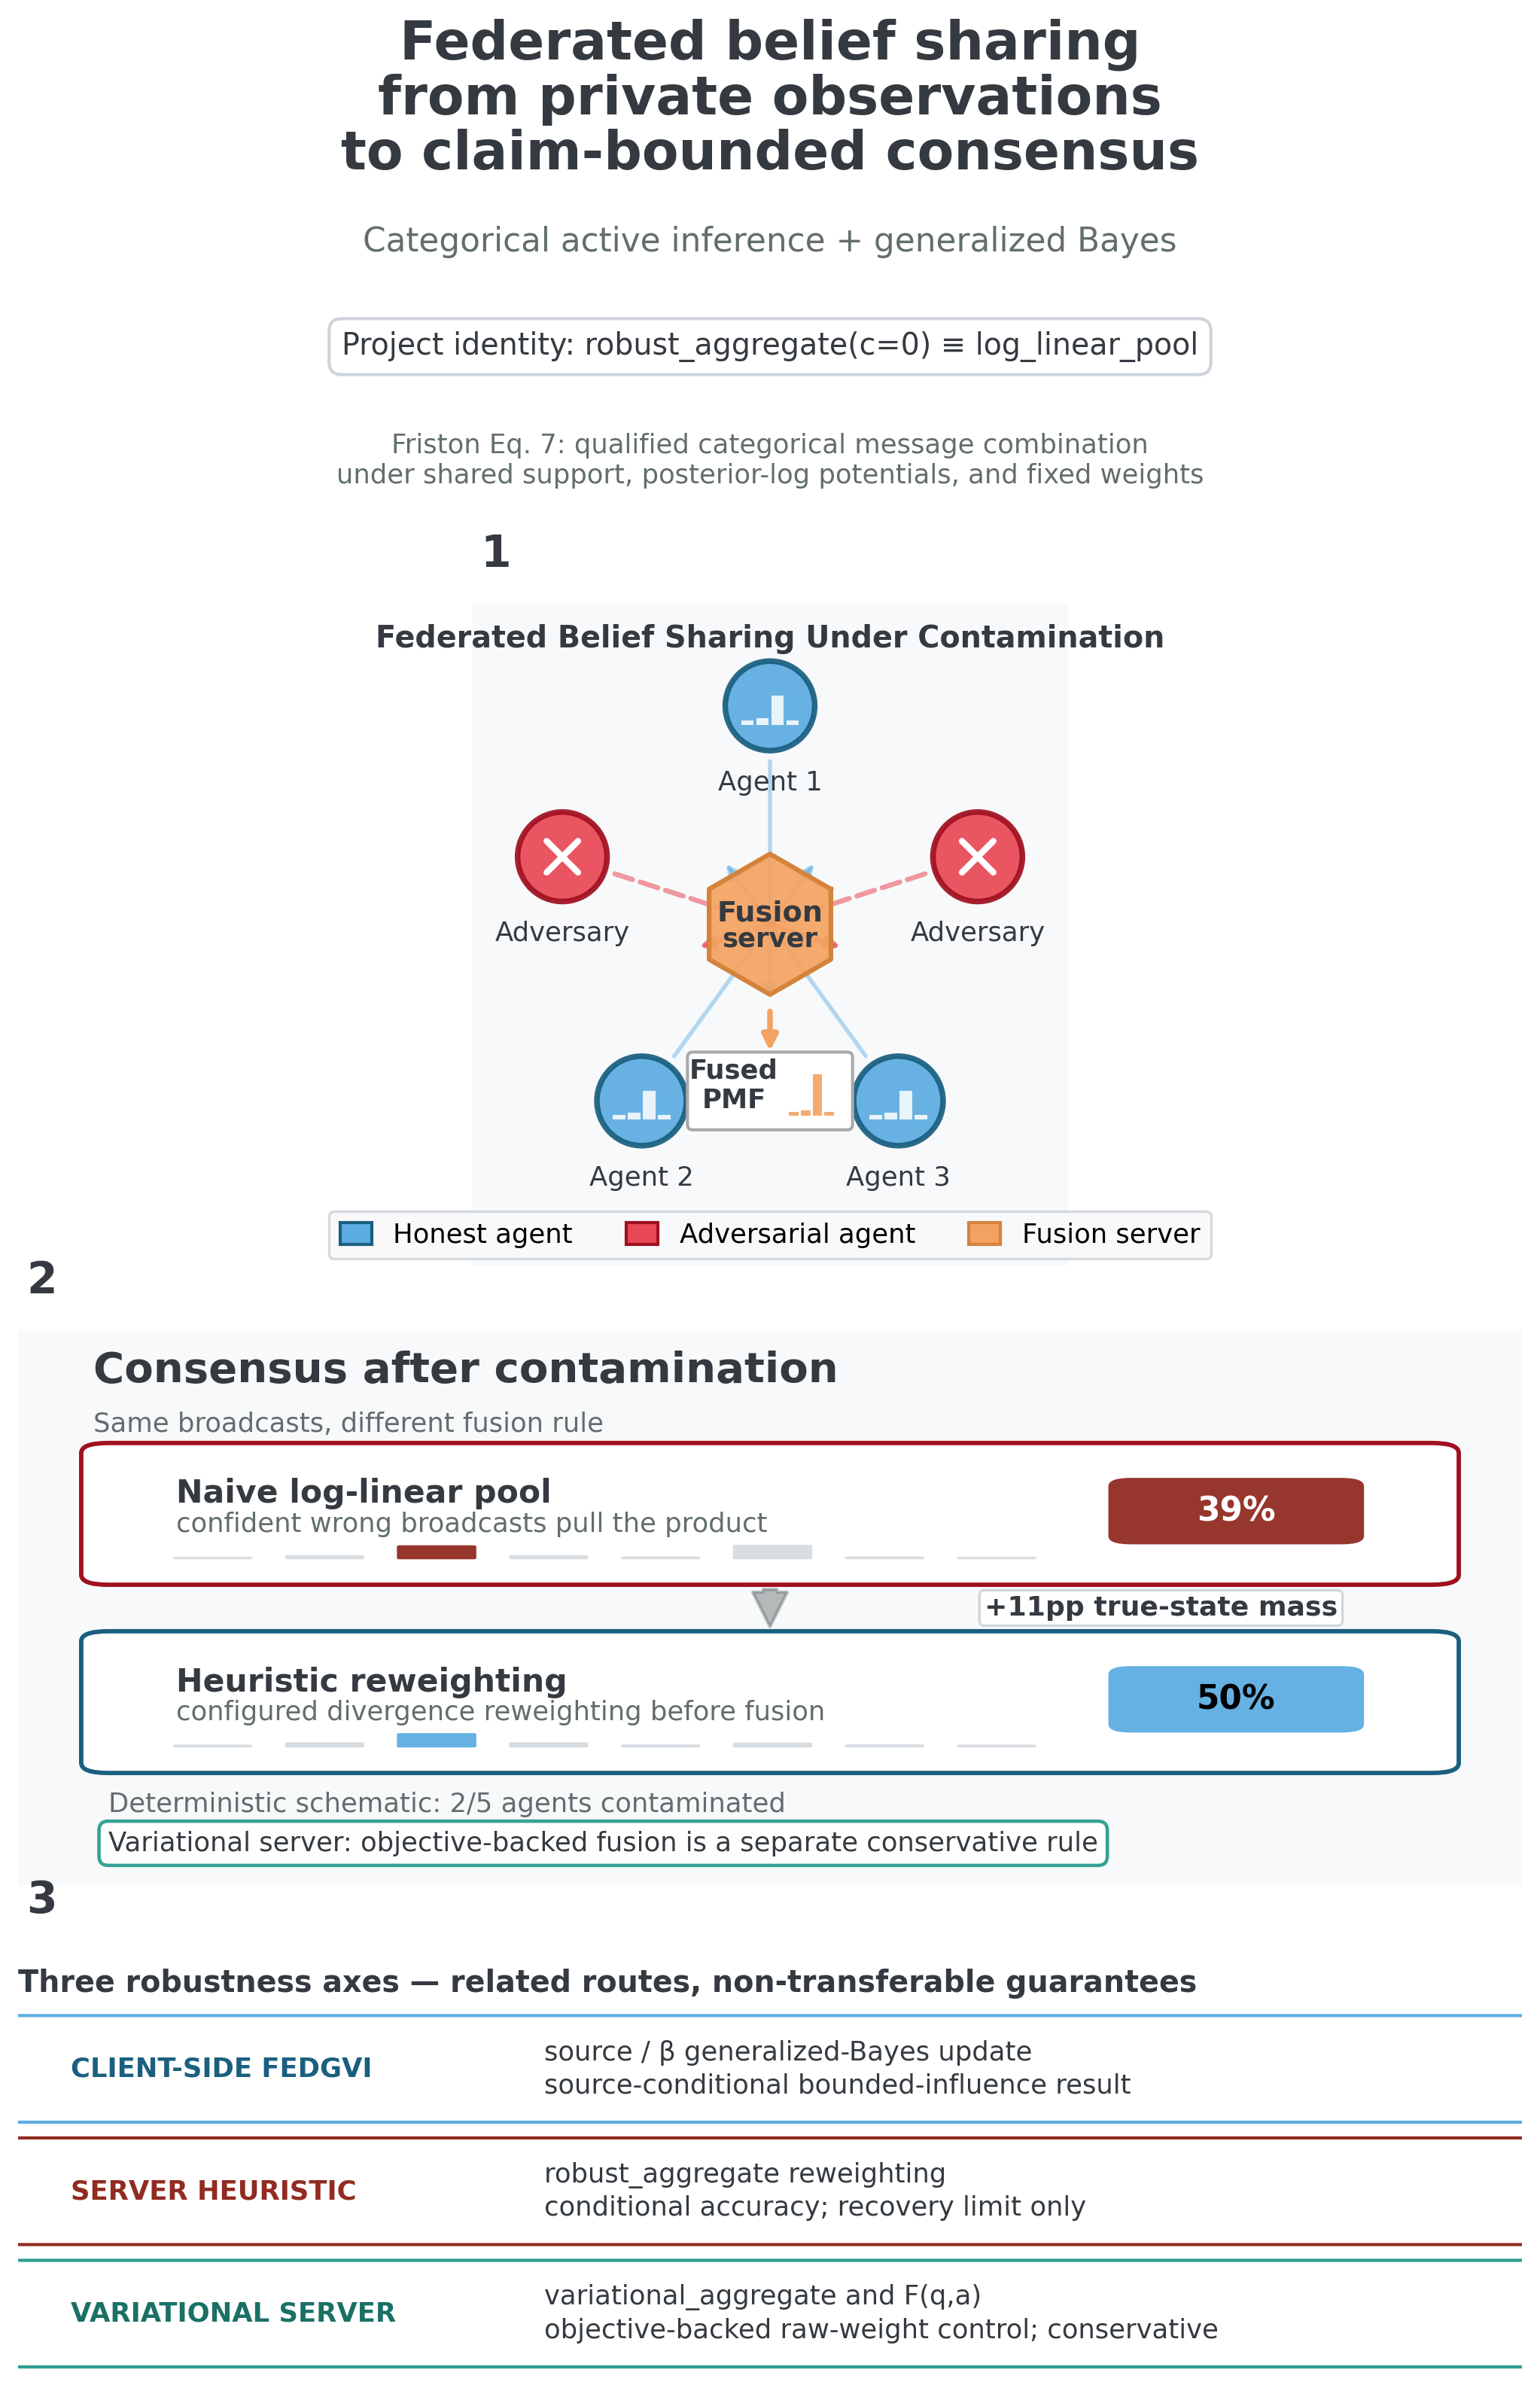
\includegraphics[width=1\linewidth,height=0.5\textheight,keepaspectratio,alt={Numbered schematic linking private categorical beliefs, honest and contaminated broadcasts, a fusion server, and three non-transferable claim lanes. Mini posterior bars with solid inbound arrows distinguish honest agents from white crosses with dashed inbound arrows. The project identity at zero server robustness is separate from the qualified categorical Eq. 7 specialization.}]{../figures/graphical_abstract.png}
\caption{Graphical abstract. Source relation: original project
formal/mechanistic schematic with configured colony and outcome
summaries; estimand: component relationships, recovery boundaries, and
the displayed true-state probability mass under two server rules. Read
from the federated network through the consensus cards to the
claim-owner strip. The x-axis is agent position in the ring or the
left-to-right comparison order; y-axis/rows encode each agent's
categorical posterior mass and the three distinct robustness lanes.
White mini posterior bars with solid inbound arrows identify honest
agents, whereas white crosses with dashed inbound arrows identify
adversarial broadcasts; direct method labels, percent badges, keylines,
and numbered reading order duplicate color. The project-local identity
\protect\texttt{robust\_aggregate(c=0)\ \texorpdfstring{\ensuremath{\equiv}}{==}\ log\_linear\_pool} is stated
separately from the categorical specialization of the Eq. 7
message-combination term, which requires shared support, admitted
posterior-log potentials, and fixed weights. Under 40\% configured
contamination, the deterministic cards report 39\% versus 50\%
true-state mass from the beliefs shown. Units are probability mass,
agent count, or conceptual route; one configured explanatory colony
supplies no replication unit, CI, error band, or significance test. The
client theorem, heuristic server evidence, and variational
effective-weight property are non-transferable, and the schematic does
not reconstruct the complete source protocol or establish universal
robustness.}\label{fig:graphical-abstract}
\end{figure}

\section{Introduction: from belief sharing to robust generalized
Bayes}\label{sec:introduction}

A colony of active-inference agents that shares beliefs inherits both
the power and the fragility of the pool it uses: the same multiplication
of reports that sharpens an honest consensus lets a single confident,
wrong member capture it. Two research communities each hold part of the
remedy but do not, on their own, close the gap.

The active-inference community gives agents generative models, action
selection, and colony-level belief sharing. The robust- and
federated-Bayes community gives generalized objectives and aggregation
methods for inference under misspecification or contamination.

The cited literatures do not, however, provide a single tested treatment
of robust categorical belief fusion for active-inference agents. This
introduction states the problem and its evidence boundary;
sec.~\ref{sec:gap} scopes the reviewed gap, and
sec.~\ref{sec:contributions} lists the contributions together with what
each result does not establish.

\subsection{Active inference supplies generative agents and shared
beliefs}\label{sec:intro-active-inference}

Active inference casts perception, learning, and action as the
minimization of variational free energy under a generative model, a
program that grew out of the free-energy principle
\citep{friston2010free} and its process-theory implementation
\citep{friston2017active}.

In the discrete state-space setting the formalism is now standardized.
An agent carries the categorical tensors \(A\) (likelihood), \(B\)
(transitions), \(C\) (preferences), and \(D_0\) (initial priors), and
infers hidden states by minimizing variational free energy. It selects
actions by minimizing \emph{expected} free energy --- the sum of a risk
term and an ambiguity term that together trade off goal-seeking against
uncertainty-resolving behavior \citep{dacosta2020active}.

This synthesis is the substrate we build on. Mature toolboxes make it
executable at scale: pymdp provides discrete-state active inference in
Python \citep{heins2022pymdp}, and RxInfer delivers reactive message
passing for exact Bayesian inference \citep{bagaev2023rxinfer}.

The community has also moved from single agents to \emph{collectives}.
Surprise-minimizing ensembles reproduce collective animal behavior such
as schooling and flocking \citep{heins2023collective}; epistemic
communities form when agents share a generative model and exchange
evidence \citep{albarracin2022epistemic}; and collective intelligence
has been framed directly in active-inference terms
\citep{kaufmann2021collective}.

The narrow bridge studied here starts from posterior broadcasts over one
shared categorical factor --- a predator's location, say --- and forms a
project log-linear pool (eq.~\ref{eq:log-linear-pool}). Under the
explicit finite-shared-support, posterior-log-potential, and
fixed-weight assumptions of sec.~\ref{sec:method-aggregation}, that
weighted geometric pool is a specialization of Friston et al.'s Eq. 7
message-combination term \citep{friston2024federated}.

It is not a reconstruction of the source message construction,
scheduling, cavity policy, generative factors, or complete protocol.
That representation connects the qualified categorical bridge to the
classical logarithmic-pooling literature
\citep{genest1986combining, genest1986externally}, to modern Bayesian
treatments of log-pool weights \citep{carvalho2023logpooling}, to
product-of-experts geometry in machine learning
\citep{hinton2002products}, and to distributed Bayesian estimators
\citep{tresp2000bayesian}. In the reproduced baseline, communication
lowers mean free energy relative to the matched incommunicado condition
(sec.~\ref{sec:results-belief_sharing}).

Friston et al. \citeyearpar{friston2024federated} crystallized the
colony mechanism into three worked simulations --- communicating-colony
free-energy convergence, Dirichlet language acquisition, and Bayesian
model reduction structure emergence --- whose mechanisms motivate three
reduced categorical analogues in this repository
(sec.~\ref{sec:results-recovery}). They are not numerical or exact
protocol replications; a source-parity reconstruction remains future
work before evaluating source-level equivalence.

Alongside fusion, the community has tools for growing the model itself:
active inference connects naturally to Bayesian optimal experimental
design and model selection \citep{smith2020active}, and post-hoc
Bayesian model reduction prunes redundant structure by comparing
free-energy bounds \citep{friston2011post} --- the algebra used by our
configured BMR sign control (sec.~\ref{sec:results-emergence}).

The reviewed active-inference belief-sharing work does not
systematically characterize fusion under explicit contamination or
intentionally wrong belief broadcasts.

The log-linear pool assumes reports are compatible with the shared
generative model, while the opinion-pooling literature makes the
assumptions about independence, weights, and external Bayesian coherence
explicit \citep{genest1986combining, genest1986externally}. Fully
Bayesian aggregation sharpens the point: geometric pooling is
normatively compelling under dynamic-Bayesian rationality assumptions,
not an assumption-free robustness procedure \citep{dietrich2021fully}.

The same product geometry can be brittle: if a report assigns zero or
near-zero mass to the true state, the product can assign near-zero mass
there too. That is the failure mode tested here, not a claim that every
federation or every product pool behaves identically.

\subsection{Robust and federated Bayes supplies bounded-influence
updating}\label{sec:intro-robust-bayes}

A separate literature studies bounded-influence updating outside active
inference. \textbf{Federated learning} aggregates models trained on
decentralized data without pooling the data itself, the canonical
algorithm being FedAvg \citep{mcmahan2017communication}.

Cast probabilistically, federated and continual learning unify under
\textbf{partitioned variational inference}, in which each client owns a
factor of a global approximate posterior and the server combines factors
in natural-parameter space
\citep{bui2018partitioned, ashman2022partitioned}. This is a closely
related factor algebra expressed in a different vocabulary; the
implementation tests the correspondence in the categorical recovery
limit rather than assuming that the two settings are interchangeable.

The robustness this paper needs comes from \textbf{generalized Bayesian
inference}, which replaces the likelihood with a \emph{loss} and the KL
regularizer with a \emph{general divergence}, so that the posterior
minimizes a generalized objective rather than applying Bayes' rule
literally
\citep{bissiri2016general, jewson2018divergence, knoblauch2022generalized}.

This includes Gibbs-posterior updates \citep{jiang2008gibbs}, coarsened
or tempered posteriors that condition on neighborhoods rather than exact
data \citep{miller2018coarsening}, and learning-rate/temperature choices
designed for safe updating under misspecification
\citep{grunwald2012safe, kleijn2012misspecification}. Choosing a loss or
divergence with a bounded-influence property --- for example, the
density-power \(\beta\)-loss
\citep{basu1998robust, fujisawa2008robust, ghosh2015robust} or
generalized cross-entropy \citep{zhang2018generalized} --- can cap the
influence of a contaminated observation under the corresponding
assumptions.

\textbf{FedGVI} \citep{mildner2025fedgvi} federates this idea: each
client runs a robust generalized-Bayes update against a \emph{cavity}
(the global posterior with the client's own factor removed), and the
server aggregates the refreshed factors under a chosen server
divergence. The result is federated inference with divergence- and
loss-specific robustness guarantees, demonstrated on Bayesian neural
networks under label contamination.

Crucially, standard Bayes is a \emph{corner} of this generalized family
--- the case where the loss is the negative log-likelihood and the
divergence is KL. Friston et al.~do not claim FedGVI, generalized Bayes,
\(\beta\)-divergence, or robustness; this manuscript supplies the
recasting.

Robust generalized Bayes therefore does not replace exact-Bayes belief
fusion; it contains the standard pool as a tested zero-robustness
recovery limit. That containment is the hinge this paper tests, and the
recovery limits are stated formally as numbered results in
sec.~\ref{sec:formalism} and the central identity in
sec.~\ref{sec:method-aggregation}.

The historical framing is deliberately modest. The manuscript uses early
probability, inverse-probability, utility, and collective-judgment
sources as a conceptual genealogy for belief, evidence, expectation, and
aggregation
\citep{pascal1654probability, huygens1657ratiociniis, bernoulli1713ars, demoivre1718doctrine, bayes1763essay, laplace1774memoire, bernoulli1738mensura, condorcet1785essai}.
These sources do not anticipate KL divergence, product-of-experts
learning, variational Bayes, or federated optimization; the modern
correspondence to FedGVI is the formal construction proved and tested
here.

Beyond this core, we evaluate a tempered objective family, a
deterministic MLP aggregation transfer, and disjoint-field-of-view
communication. These are boundary tests: the first probes the
accuracy/weight-control trade-off, the second tests API portability in
one additional model class, and the third separates a binary-complement
null result from a larger-state-space case where communication
materially improves consensus.

\subsection{Questions, design, and evidence
boundary}\label{sec:intro-questions}

The paper answers four scoped questions. First, does turning robustness
off recover the standard log-linear pool and closed-form Bayes update?
Second, under the declared confident-wrong broadcast mechanism, how does
the server heuristic change consensus accuracy across contamination
rates? Third, what does the objective-backed variational server rule
guarantee, and what accuracy does it trade away? Fourth, how do
communication, hierarchy, sensitivity, and parameter recovery behave in
the accompanying categorical extensions?

The first question is answered algebraically and by machine-precision
checks; the others are conditional simulation results. The independent
unit, resampling scheme, and fixed hidden-state/attack-target estimand
are specified in sec.~\ref{sec:methods-experimental-design} and
sec.~\ref{sec:methods-statistics}.

\subsubsection{How to read the visual
architecture}\label{sec:intro-visual-map}

The manuscript uses two complementary visual layers. The formal
schematics adapt the generative-model and posterior-sharing perspective
of Friston et al. \citeyearpar{friston2024federated} to the categorical
implementation: fig.~\ref{fig:generative-model-schema} shows the private
sensory report and \(A/B/C/D\) substrate, fig.~\ref{fig:message-passing}
shows how three local posterior messages become server inputs, and
fig.~\ref{fig:pomdp-loop} shows the hidden-state, agent, and
active-control context. These diagrams are explanatory maps, not
additional empirical observations.

The data-bearing figures then report the executed recovery checks,
conditional contamination sweep, and objective/descent diagnostics;
their captions identify the relevant uncertainty and resampling unit.
The graphical abstract in fig.~\ref{fig:graphical-abstract} compresses
the same logic into a recovery anchor, a federation pathway, and three
explicitly non-transferable robustness axes.

fig.~\ref{fig:system-overview} illustrates one configured
failure-and-repair case: a partially contaminated colony broadcasts
beliefs (Panel A), the equal-weight log-linear pool is pulled toward the
attack target (Panel B), and the server-side heuristic reweights the
broadcasts (Panel C). It is a deterministic schematic, not a universal
robustness claim; the three axes and their distinct guarantees are
defined in sec.~\ref{sec:gap} and sec.~\ref{sec:robustness-axes}.

\begin{figure}
\centering
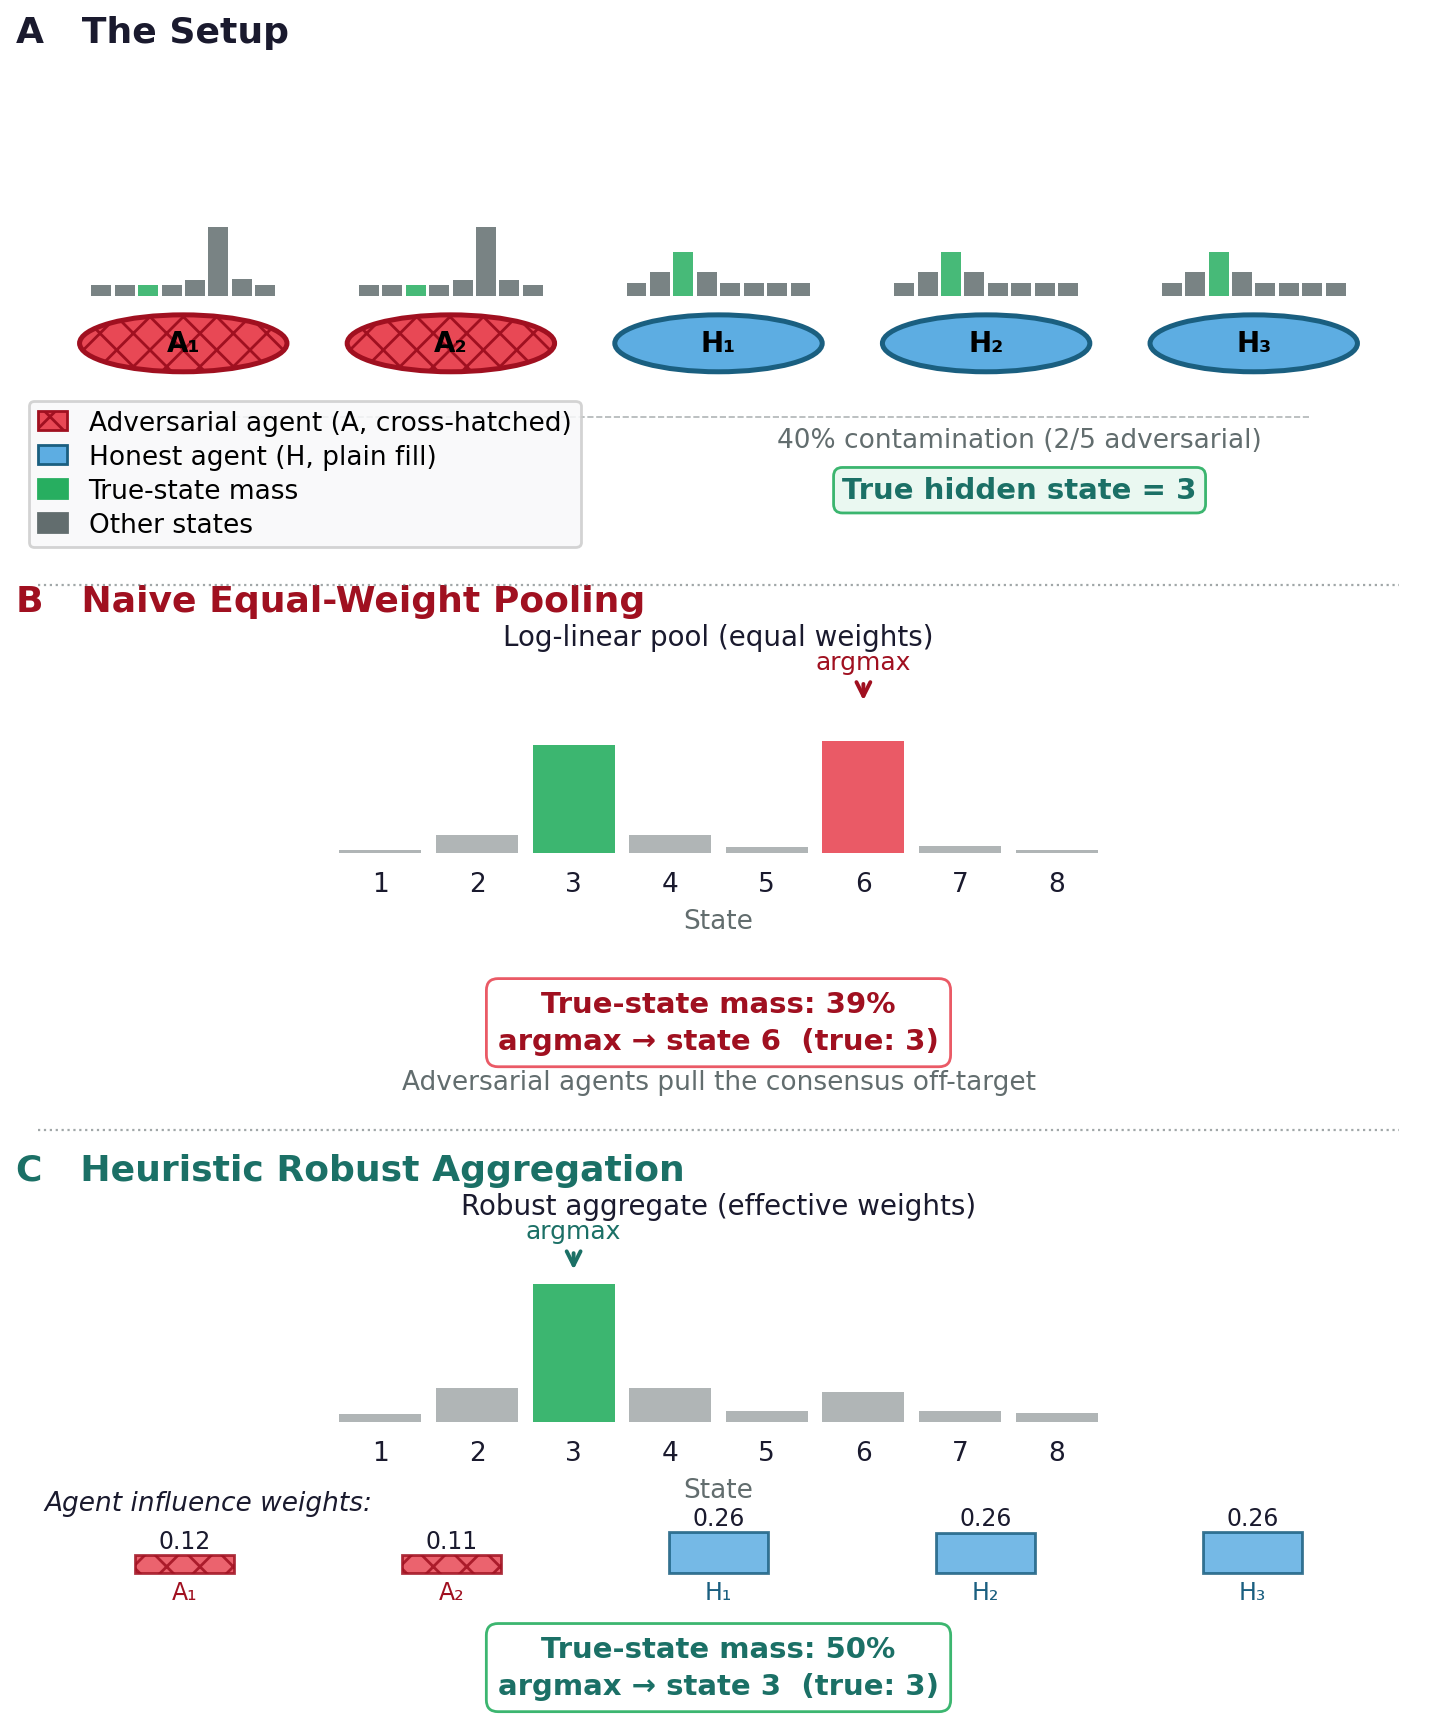
\includegraphics[width=1\linewidth,height=0.5\textheight,keepaspectratio,alt={Three-part configured diagnostic of a five-agent colony with two A-labeled adversarial and three H-labeled honest agents, naive equal-weight pooling, and heuristic reweighting. Cross-hatched A roles and plain-filled H roles have distinct keylines; direct state, argmax, true-state-mass, agent-role, and influence-weight labels show the off-target naive outcome and displayed heuristic recovery without color.}]{../figures/system_overview.png}
\caption{System overview of one configured failure-and-repair
diagnostic. Source relation: original project schematic computed from
the displayed colony; estimand: posterior-mass and normalized
influence-weight contrasts. Read Panels A--C from the five heterogeneous
local posteriors, through naive equal-weight pooling, to canonical
\protect\breaktt{robust\_aggregate} heuristic reweighting. The x-axis is
hidden-state index 1--8 in Panels B and C; the y-axis is posterior
probability mass, while the influence bars report normalized server
weight. Cross-hatched A\texorpdfstring{\textsubscript{1}}{1}/A\texorpdfstring{\textsubscript{2}}{2} roles with adversarial keylines and
plain-filled H\texorpdfstring{\textsubscript{1}}{1}--H\texorpdfstring{\textsubscript{3}}{3} roles with honest keylines distinguish agents
without color; numbered states, true-state text, argmax arrows,
per-agent weight labels, and direct percentages identify every outcome.
The true hidden state is 3. Under 40\% configured contamination, the
equal-weight pool assigns 39\% mass to the true state and its argmax
lands on the adversarial state, whereas the heuristic assigns 50\% and
recovers the displayed true-state argmax. Units are probability mass and
normalized weight. This single deterministic colony has no independent
replication unit, resampling interval, error bar, or CI; its failure and
repair do not establish calibrated uncertainty, universal heuristic
robustness, or the variational server's objective-backed weight-control
result.}\label{fig:system-overview}
\end{figure}

\section{Research gap and claim boundary}\label{sec:gap}

The two communities of sec.~\ref{sec:introduction} provide substantial
pieces of the problem, but the cited threads do not answer the same
question. The gap is not a claim that either field is incomplete; it is
the untested intersection between active-inference belief sharing and
robust generalized Bayes. This section describes that intersection
thread by thread, states the scoped bridge evaluated here, and records
the evidence boundary that travels with it.

\subsection{Five reviewed threads and their open
intersection}\label{sec:gap-threads}

Five threads in the reviewed literature run toward the gap but do not,
in the sources cited here, cross it --- three from active inference and
two from robust Bayes.

\textbf{Thread 1 --- Generative modeling and action} (active inference).
Discrete active inference is a mature, synthesized formalism with
standardized tensors and an expected-free-energy action rule
\citep{friston2010free, dacosta2020active}, and it is executable at
scale through pymdp \citep{heins2022pymdp} and RxInfer
\citep{bagaev2023rxinfer}. \emph{Boundary:} these sources do not by
themselves equip the active-inference inference step with the
contamination mechanism evaluated here.

\textbf{Thread 2 --- Collective belief coordination} (active inference).
Colonies coordinate by sharing beliefs and minimizing collective
surprise, reproducing flocking \citep{heins2023collective},
epistemic-community formation \citep{albarracin2022epistemic}, and
collective intelligence \citep{kaufmann2021collective}. \emph{Boundary:}
the cited collective-belief studies treat the broadcast posteriors as
trusted and do not evaluate the robustness of fusion to misspecified or
intentionally wrong members.

\textbf{Thread 3 --- Belief sharing and structure growth} (active
inference). Federated belief sharing fuses posteriors into a hive-mind
consensus \citep{friston2024federated}, and post-hoc Bayesian model
reduction \citep{friston2011post} together with optimal-design-flavored
model selection \citep{smith2020active} grow and prune the generative
model. \emph{Boundary:} in the cited belief-sharing line, fusion is
exact-Bayes and trusting; its connection to the robustness theory
developed for federated learning is not evaluated.

\textbf{Thread 4 --- Federated and partitioned inference} (robust
Bayes). Federated learning aggregates decentralized models
\citep{mcmahan2017communication}, and partitioned variational inference
gives the factor-algebra framework that unifies federated and continual
learning \citep{bui2018partitioned, ashman2022partitioned}.
\emph{Boundary:} the cited examples target parameter or predictive-model
factors rather than the generative-model-bearing, action-selecting POMDP
belief consensus used here.

\textbf{Thread 5 --- Generalized and robust Bayes} (robust Bayes).
Generalized Bayesian updating replaces the likelihood--KL pair with a
loss--divergence pair
\citep{bissiri2016general, knoblauch2022generalized}; bounded losses ---
the density-power \(\beta\)-divergence \citep{basu1998robust} and
generalized cross-entropy \citep{zhang2018generalized} --- deliver
bounded influence; and FedGVI \citep{mildner2025fedgvi} federates the
robust objective with provable guarantees.

\emph{Boundary:} the cited robust-Bayes apparatus does not evaluate
active-inference POMDP belief consensus. Its behavior in the discrete
categorical regime of the worked belief-sharing example
\citep{friston2024federated} is the scoped setting evaluated here.

\subsection{The belief-fusion bridge evaluated
here}\label{sec:gap-bridge}

Across these reviewed threads, the missing intersection is specific. The
cited active-inference sources provide belief fusion but not the
contamination analysis used here. The cited robust-Bayes sources provide
robust inference but not this acting-agent categorical consensus. We
evaluate a bridge comprising three distinct robustness axes and one
recovery anchor.

The client axis is a FedGVI-faithful generalized-Bayes update using the
\(\beta\)- and rcce-losses (eq.~\ref{eq:beta-loss},
eq.~\ref{eq:rcce-loss}). The heuristic server axis reweights each agent
by divergence from the current consensus (eq.~\ref{eq:robust-identity}).
The objective-backed server axis is a conservative variational rule with
a stated aggregation free energy and raw effective-weight bound
(eq.~\ref{eq:agg-free-energy}).

The shared anchor recovers the standard-Bayes client limit and project
log-linear-pool server identity (sec.~\ref{sec:formalism-recovery}).
Under the qualified bridge of sec.~\ref{sec:method-aggregation}, the
latter specializes Friston et al.'s Eq. 7 message-combination term
\citep{friston2024federated}, not the complete source protocol. The
algebra and executable residuals identify a recovery boundary, not an
equivalence of literatures.

Declared comparisons use paired Wilcoxon statistics
\citep{wilcoxon1945individual}, Benjamini--Hochberg FDR
\citep{benjamini1995controlling}, percentile-bootstrap intervals
\citep{efron1993bootstrap}, and observed-effect design-power planning.
Source-bound reports make those analyses reproducible
\citep{peng2011reproducible}; they do not promote a conditional
simulation into a theorem.

\subsection{Guarantee map: three robustness
axes}\label{sec:robustness-axes}

A red-team review surfaced the paper's authoritative robustness
taxonomy. Robustness enters in \textbf{three} places, with different
claim owners, evidence classes, and permitted interpretations.

\subsubsection{Client-side:
source-theorem-backed}\label{client-side-source-theorem-backed}

The per-agent generalized-Bayes update uses a bounded loss inside
\breaktt{generalized\_posterior} (eq.~\ref{eq:beta-loss},
eq.~\ref{eq:rcce-loss}). It is derived from eq.~\ref{eq:gen-bayes} and
limits to NLL/Bayes as the loss parameter approaches zero (Corollary
\ref{cor:closed-form-bayes}; Proposition
\ref{prop:robust-loss-recovery}). FedGVI's bounded-influence result
transfers only under the source theorem's loss, model, and contamination
assumptions \citep{mildner2025fedgvi}.

\subsubsection{Server-side: heuristic}\label{server-side-heuristic}

\breaktt{robust\_aggregate} discounts an agent by
\(\exp(-c\,\mathrm{KL}(q_n \,\|\, q))\). Its proved positive property is
the recovery limit: at \(c=0\), it equals the standard log-linear pool
(eq.~\ref{eq:robust-identity}, Theorem
\ref{thm:belief-sharing-recovery}). It is not a closed-form
FedGVI-objective minimizer and does not inherit the client-side
bounded-influence result.

\subsubsection{Server-side: objective-backed and
conservative}\label{server-side-objective-backed-and-conservative}

\breaktt{variational\_aggregate} applies exact block updates that do not
increase the stated free energy eq.~\ref{eq:agg-free-energy}. It
recovers the log-linear pool in the trusting limit and bounds each raw
effective weight by its base weight. Its declared tradeoff is a
conservative consensus; the objective-backed property does not imply
peak-accuracy dominance.

The robustness results (sec.~\ref{sec:results-robustness}) apply this
map, and sec.~\ref{sec:limitations-scope} states the complete boundary.
Effect sizes, intervals, and planning quantities characterize the server
heuristic's conditional behavior; they do not transfer the client
theorem or variational objective to that heuristic. Later sections refer
back to this taxonomy rather than redefine it.

\section{Contributions and evidence boundaries}\label{sec:contributions}

We make ten contributions, each paired with a theorem, figure, table, or
generated token and with an explicit boundary on what the evidence
establishes.

They fall into four groups: the first two build the core and its
recovery contract; the next two report and statistically qualify the
contaminated-consensus result; the fifth and sixth make the robustness
axes explicit and add the objective-backed server rule; and the
remaining four are scoped extensions --- parameter recovery, the
tempered aggregation family, an aggregation-API transfer, and a
disjoint-observation communication test.

\subsection{1. A discrete-categorical FedGVI
core}\label{a-discrete-categorical-fedgvi-core}

A typed, deterministic, pure-NumPy/SciPy reimplementation of the FedGVI
\citep{mildner2025fedgvi} generalized-Bayes primitives --- divergences,
bounded robust losses, the generalized posterior, the cavity/factor
algebra, and robust aggregation --- in the discrete-categorical setting
that active inference \citep{dacosta2020active} uses.

The objective (eq.~\ref{eq:gen-bayes}) and its closed-form
tempered-softmax solution are stated in Definition
\ref{def:generalized-bayes} and tested by the recovery-limit probes. The
whole core is zero-mock and reproducible \citep{peng2011reproducible}.

\subsection{2. A recovery-tested connection between categorical pooling
and robust
Bayes}\label{a-recovery-tested-connection-between-categorical-pooling-and-robust-bayes}

A recovery certificate shows that the client KL/negative-log-likelihood
loss limits recover Bayes and the server's zero-robustness branch
recovers the project log-linear pool.

Under the explicit shared-support, posterior-log-potential, and
fixed-weight assumptions in sec.~\ref{sec:method-aggregation}, that pool
specializes Friston et al.'s Eq. 7 message-combination term
\citep{friston2024federated}, not the complete source protocol.

Three recovery limits are pinned to bit-level residuals. The bounded
losses recover NLL/Bayes (Corollary \ref{cor:closed-form-bayes} +
Proposition \ref{prop:robust-loss-recovery}; \(\le 0\) and \(\le 0\)
maximum residual, eq.~\ref{eq:standard-bayes}).

The Rényi divergence recovers KL (Lemma \ref{lem:renyi-kl-limit};
\(\le 0\) residual, eq.~\ref{eq:renyi-limit}). The server-side
reweighting pool recovers the naive pool in its trusting limit (Theorem
\ref{thm:belief-sharing-recovery}; \(\le 0\) residual,
eq.~\ref{eq:robust-identity}).

Robustness is thereby a tested recovery-limit extension, not a
replacement.

\subsection{3. End-to-end evaluation of robust federated active
inference}\label{end-to-end-evaluation-of-robust-federated-active-inference}

Three worked categorical source-mechanism analogues cover communicating
colonies reaching lower free energy
(sec.~\ref{sec:results-belief_sharing}), Dirichlet language acquisition
(sec.~\ref{sec:results-language}), and a configured Bayesian-model-
reduction pruning sign control \citep{friston2011post}
(sec.~\ref{sec:results-emergence}).

A contaminated-sentinel robustness sweep
(sec.~\ref{sec:results-robustness}) shows the naive pool degrading while
at least one server-side robust member clears the configured threshold
at the most severe swept rate.

\subsection{4. A statistically qualified server-side
contrast}\label{a-statistically-qualified-server-side-contrast}

The ``robust beats naive'' conclusion for the declared contamination
rate is produced only by a matched-pairs Wilcoxon signed-rank test
\citep{wilcoxon1945individual}. Its multiplicity correction uses
Benjamini--Hochberg FDR \citep{benjamini1995controlling} across the
divergence family. We report the contrast with bootstrap confidence
intervals \citep{efron1993bootstrap} and observed-effect design-power
planning.

Across 960 paired trials, the headline display method (RKL; tied set:
RKL, AR, beta, rcce) reaches accuracy 0.9829 against the naive pool's
0.9021 at the verdict rate.

At that rate, \(q = 1.11 \times 10^{-158}\), and the
rank-biserial-derived \(d\)-equivalent is saturated (r=+1). The
predeclared selection rule is largest positive rank-biserial
effect\_size; stable method order tie-break; the method with the largest
paired mean difference is AR. Every headline number is a generated
token.

\subsection{5. An explicit accounting of the robustness
axes}\label{an-explicit-accounting-of-the-robustness-axes}

The map in sec.~\ref{sec:robustness-axes} separates the client-side
per-agent update, which inherits FedGVI's bounded-influence result under
its stated source assumptions, from both server rules.

The sharp server-side reweighting heuristic has a recovery limit as its
positive formal property and a scoped no-go result for its declared
separable objective class.

The conservative variational server rule is objective-backed and has a
redescending effective-weight update, but is not the accuracy-maximizer.
Downstream users are told exactly which result is theoretically backed
and which is a labeled heuristic.

\subsection{6. An objective-backed server aggregator with redescending
weights}\label{an-objective-backed-server-aggregator-with-redescending-weights}

We derive an aggregation free energy eq.~\ref{eq:agg-free-energy} whose
exact block updates define the \breaktt{variational\_aggregate} rule
(sec.~\ref{sec:method-variational}, sec.~\ref{sec:supp-variational}).

Each exact block update monotonically decreases a stated objective, and
a converged fixed point is coordinatewise stationary. The implementation
keeps the lowest observed objective among converged configured starts,
or reports the best unfinished trace as non-converged.

The rule recovers the standard log-linear pool in the trusting limit
(eq.~\ref{eq:robust-identity}) and --- unlike the sharp heuristic ---
carries a proven raw effective-weight bound
(fig.~\ref{fig:aggregation-descent}, fig.~\ref{fig:bounded-influence}).

The honest cost is conservatism: it is a maximum-entropy-biased
consensus and trades peak point-accuracy for that control, so it
complements rather than replaces the sharp heuristic of contribution 5.

\subsection{7. Executed finite-grid acuity-recovery
experiment}\label{executed-finite-grid-acuity-recovery-experiment}

At each value in the 0.60, 0.70, 0.80, 0.90 acuity grid, the study
generates 200 synthetic observations in each of 960 trials. It selects
acuity by marginal-likelihood grid search over the declared finite grid.

The observed mean absolute error is 0.0232 with \(R^2 = 0.9999\)
(fig.~\ref{fig:parameter-recovery}). Acuity-by-colony-size behavior
belongs to the separate sensitivity study; it is not a
parameter-recovery result.

\subsection{8. The tempered aggregation
family}\label{the-tempered-aggregation-family}

A one-parameter \(\lambda>0\) generalization of the variational
aggregate (sec.~\ref{sec:supp-tempered}) is the objective

\begin{equation}\protect\phantomsection\label{eq:contribution-tempered-family}{
\begin{aligned}
F_\lambda(q,a)
&= \sum_n a_n\,\mathrm{CE}(q,q_n)-\lambda H(q)\\
&\quad +\frac{1}{c}\,\mathrm{KL}_{\mathrm{gen}}(a\Vert w).
\end{aligned}
}\end{equation}

In eq.~\ref{eq:contribution-tempered-family}, at \(\lambda = 1.0\), the
temperature is unity and the objective reduces to the standard
variational aggregate bit-for-bit. Lower \(\lambda\) sharpens the
variational \(q\)-block toward a maximizing state; it does not
algebraically recover \breaktt{robust\_aggregate}.

The raw effective-weight update and its bound are preserved for all
\(\lambda\). The full derivation is in sec.~\ref{sec:supp-tempered}.

\subsection{9. An aggregation-API transfer
demonstration}\label{an-aggregation-api-transfer-demonstration}

The same \breaktt{robust\_aggregate} API that governs the POMDP studies
is exercised unchanged with one deterministic MLP trained with the
density-power \(\beta\)-loss (16 hidden units, \(\beta=0.5\);
generalized variational inference with a point-mass variational family)
as the per-client model.

This supports portability of the server API to one additional model
class (sec.~\ref{sec:results-baseline}) when the optional \texttt{torch}
extra is installed (sec.~\ref{sec:methods-software}). Without it, the
MLP run is skipped and its tokens render accordingly.

\subsection{10. Communication contrast under disjoint
observations}\label{communication-contrast-under-disjoint-observations}

A multi-agent extension (sec.~\ref{sec:results-disjoint-fov}) in which 3
agents each observe a 2-slot disjoint window shows that belief sharing
materially improves over isolated-agent accuracy in the declared
configuration. Isolated agents clear the 0.167 chance baseline but stay
far below the communicating consensus, which itself remains well short
of full accuracy.

Across 128 seeds, isolated accuracy is 0.326 versus communicating 0.493,
a reproducible margin under the declared matched-seed comparison
(Wilcoxon \(p = 9.35 \times 10^{-23}\)). This is evidence for the
configured disjoint-observation protocol, not a universal communication
theorem.

The remainder of the paper proceeds as follows. sec.~\ref{sec:methods}
develops the FedGVI core and the recovery limits;
sec.~\ref{sec:formalism} states the numbered recovery theorems and the
expected-free-energy identity;
sec.~\ref{sec:methods-experimental-design} fixes the configuration;
sec.~\ref{sec:results} reports the 9 studies, beginning with the
recovery checks (sec.~\ref{sec:results-recovery}).

sec.~\ref{sec:discussion} and sec.~\ref{sec:conclusion} synthesize; and
sec.~\ref{sec:reproducibility} and sec.~\ref{sec:limitations-scope}
document determinism, scope, limitations, and the standing of each
robustness axis.

\section{Methods: the federated active-inference
stack}\label{sec:methods}

\protect\phantomsection\label{sec:methodology}{}

This section develops the federated generalized variational inference
(FedGVI) core in the discrete-categorical setting and defines its
primitives. Their recovery limits are stated as numbered theorems in
sec.~\ref{sec:formalism}. Every belief here is a categorical pmf --- a
non-negative vector summing to one --- so the
generalized-variational-inference machinery reduces to closed forms that
are exactly testable.

All mathematics lives in \texttt{src/fedference/}; the prose names the
module and the identity that pins each claim.

The active-inference community has built a rich apparatus for federated
belief sharing: discrete-state-space agents that broadcast posteriors
and fuse them into a consensus
\citep{dacosta2020active, friston2024federated}, message-passing
toolboxes that make exact-Bayes inference scalable
\citep{heins2022pymdp, bagaev2023rxinfer}, and collective and
multi-agent formulations in which ensembles coordinate by sharing
observations and beliefs
\citep{heins2023collective, albarracin2022epistemic, kaufmann2021collective}.

We accept that apparatus and extend it. Among the active-inference
sources reviewed here, the consensus rules are exact-Bayes and trusting,
without an account of an ensemble member that is misspecified or
adversarial.

Outside active inference, the federated-learning and robust-Bayes
literatures address important parts of that question --- decentralized
aggregation \citep{mcmahan2017communication}, partitioned and federated
variational inference \citep{ashman2022partitioned, bui2018partitioned},
and generalized, robustness-bearing Bayesian updating
\citep{bissiri2016general, knoblauch2022generalized, basu1998robust, zhang2018generalized}.
Among the sources reviewed here, that apparatus has not been carried
into the generative-model-bearing, action-selecting POMDP setting. The
methodology below is the bridge.

It federates the FedGVI objective \citep{mildner2025fedgvi} per agent
inside an active-inference ensemble, proves the standard-Bayes client
limits, and tests the project-local zero-robustness log-linear-pool
identity. Under the qualified categorical bridge of
sec.~\ref{sec:method-aggregation}, that pool specializes Eq. 7's
message-combination term rather than the complete source protocol.
fig.~\ref{fig:system-overview} illustrates the three-axis architecture
and the recovery hierarchy.

\subsection{Federation protocol: local update, server fusion,
broadcast}\label{sec:method-protocol}

A colony of \(N\) agents shares a single latent factor
\(s \in \{1,\dots,n_s\}\) (in the sentinel scenario, the location of a
creature on a grid of \(n_s\) cells). Each round proceeds in three
steps:

\subsubsection{1. Local inference}\label{local-inference}

Agent \(n\) observes \(o_n\) and forms a local posterior \(q_n(s)\) over
the shared factor by a generalized-Bayes update against its own cavity,
the colony belief with agent \(n\)'s previous contribution removed.

This is where robustness enters per agent: the update minimizes a
loss-plus-divergence objective, and the FedGVI choice of a bounded loss
carries the source theorem's bounded-influence result under its matching
assumptions.

\subsubsection{2. Broadcast}\label{broadcast}

Agent \(n\) broadcasts \(q_n(s)\), optionally with a scalar base weight
\(w_n \ge 0\).

\subsubsection{3. Aggregation}\label{aggregation}

The server, or equivalently each agent acting as its own server, fuses
the broadcast beliefs into a consensus. Following sensory attenuation
--- ``agents do not hear themselves'' --- an agent's heard consensus
excludes its own message.

The protocol has two distinct places where robustness can live, and we
keep them separate throughout. The \textbf{per-agent generalized-Bayes
update} in step 1 is FedGVI-faithful at the stated primitive level: its
formal bounded-influence claim is conditional on the source theorem's
assumptions.

The \textbf{server-side aggregation rule} in step 3 admits an optional
divergence-reweighting heuristic that down-weights agents far from the
emerging consensus; this heuristic is a complementary device whose
positive formal property is recovery of the naive consensus in its
trusting limit, while a scoped proposition rejects one declared
separable objective class.

sec.~\ref{sec:robustness-axes} holds this boundary; no figure, table, or
sentence in this work grants the server-side heuristic the per-agent
FedGVI guarantee.

\subsection{Notation for beliefs, losses, and
divergences}\label{sec:method-notation}

The authoritative symbol and API contract is
sec.~\ref{sec:supp-notation}. In the main text, \(q_n(s)\) denotes agent
\(n\)'s local posterior, \(q(s)\) the global consensus, and
\(q_{-n}(s)\) the cavity after removing the site factor \(t_n(s)\).

The prior is \(\pi_0(s)\), while \(\boldsymbol{\pi}\) is a policy. The
POMDP tensors are \(A[o,s]\), \(B[s',s,u]\), \(C[o]\), and \(D_0[s]\).

The aggregation weights are \(w_n\) (raw/base), \(a_n\) (raw variational
effective), and \(\widetilde a_n\) (normalized influence). The server
robustness coefficient is \(c\), the variational entropy weight is
\(\lambda\), the Rényi order is \(\alpha\), the density-power parameter
is \(\beta\), and the robust cross-entropy parameter is
\(q_{\text{loss}}\). The notation supplement also defines the seed/trial
nesting and all statistical quantities used below.

The study is run over a fixed ensemble of 7 agents sharing a factor of 9
locations, with all randomness seeded at 0; the full per-study
configuration is tabulated in tbl.~\ref{tbl:study_params}. As an
independent generative-model-free baseline, we also implement FedGVI in
a deterministic MLP complement trained with the density-power
\(\beta\)-loss --- generalized variational inference with a point-mass
variational family (sec.~\ref{sec:results-baseline}).

The remaining methodology subsections develop each primitive in turn:
the generalized-Bayes update and its recovery to standard Bayes
(sec.~\ref{sec:method-genbayes}), the divergence family and its KL limit
(sec.~\ref{sec:method-divergences}) and the robust loss family and its
NLL limit (sec.~\ref{sec:method-losses}), the aggregation identity
(sec.~\ref{sec:method-aggregation}), the lift to a belief-sharing round
(sec.~\ref{sec:method-belief-sharing}), and the paired statistics that
earn every ``robust beats naive'' verdict
(sec.~\ref{sec:methods-statistics}).

\subsection{Generalized Bayes: the route back to standard
Bayes}\label{sec:method-genbayes}

The inference engine FedGVI federates is the generalized (Gibbs)
posterior
\citep{bissiri2016general, jiang2008gibbs, jewson2018divergence, knoblauch2022generalized},
which trades the likelihood for a loss \(L\) and the KL regularizer for
a general divergence \(\mathcal D\):

\begin{equation}\protect\phantomsection\label{eq:gen-bayes}{
\begin{aligned}
q_n^\ast(s)
&= \arg\min_{q_n}
\left\{
\begin{aligned}
&\mathbb{E}_{q_n}\!\Big[\textstyle\sum_i L(s; o_i)\Big]\\
&\quad + \tfrac{1}{\tau}\,\mathcal D\!\big(q_n \,\|\, \pi_0\big)
\end{aligned}
\right\}.
\end{aligned}
}\end{equation}

with prior \(\pi_0\), learning rate \(\tau\), and regularizing
divergence \(\mathcal D\). The learning rate is part of the inferential
specification, not a cosmetic constant; coarsened-posterior and
safe-Bayes work show why calibration of that temperature matters under
misspecification \citep{miller2018coarsening, grunwald2012safe}, where
ordinary Bayes concentrates around a KL pseudo-truth rather than literal
truth when the model family is wrong \citep{kleijn2012misspecification}.
We name the object eq.~\ref{eq:gen-bayes} defines.

\begin{definition}[Generalized-(Gibbs)-Bayes posterior]\label{def:generalized-bayes}
Given loss $L$, prior $pi_0$, learning rate $tau>0$, and divergence
$\mathcal D$, the generalized-Bayes posterior $q_n^\ast$ minimizes
(\ref{eq:gen-bayes}). When $\mathcal D=\mathrm{KL}$, its exact categorical
minimizer is the tempered softmax in (\ref{eq:tempered-softmax}).
\end{definition}

\begin{equation}\protect\phantomsection\label{eq:tempered-softmax}{
q_n^\ast(s) \;\propto\; \pi_0(s)\,\exp\!\big(-\tau \textstyle\sum_i L(s; o_i)\big),
}\end{equation}

The implementation surface is the \breaktt{generalized\_posterior}
function in the \breaktt{generalized\_bayes} module.

The tempered softmax of eq.~\ref{eq:tempered-softmax}, stated in the
definition above, is not an approximation: it is the exact closed-form
minimizer of eq.~\ref{eq:gen-bayes} when the regularizer is the KL
divergence, because the categorical support is finite and the objective
is strictly convex in \(q\). The recovery to standard Bayes follows by
choosing the loss.

With \(L=\mathrm{NLL}\), \(\mathrm{NLL}(p, o) = -\log p(o)\), the
exponential in that tempered softmax becomes a product of likelihoods
and the minimizer is \emph{exactly} standard Bayes;
eq.~\ref{eq:standard-bayes} in sec.~\ref{sec:method-aggregation} states
that corner, and Corollary \ref{cor:closed-form-bayes} there pins it to
the closed-form prior-times-likelihood product.

The largest observed discrepancy between \breaktt{generalized\_posterior}
in this regime and the analytic Bayes posterior is 5.55e-17, reported in
sec.~\ref{sec:results-recovery} --- exact to machine precision (a
maximum deviation of about one ULP), not merely close.

FedGVI computes each client update against a \emph{cavity} rather than
the full posterior, so a contributing agent does not double-count its
own previous message. We name that operation.

\begin{definition}[Cavity / PVI factor update]\label{def:cavity}
The cavity is the normalized removal of agent $n$'s site factor from the colony
posterior in natural-parameter space, as in (\ref{eq:cavity}). PVI replaces the
site factor and recombines it with that cavity according to
(\ref{eq:factor-replacement}).
\end{definition}

\begin{equation}\protect\phantomsection\label{eq:cavity}{
\begin{aligned}
q_{-n}(s)
&=
\frac{q(s)/t_n(s)}{\sum_{s'} q(s')/t_n(s')}
\\
&=
\operatorname{softmax}\!\big(\log q(s)-\log t_n(s)\big),
\end{aligned}
}\end{equation}

The final expression makes normalization explicit. Taking a cavity and
re-multiplying the original site factor restores the global posterior:

\begin{equation}\protect\phantomsection\label{eq:factor-replacement}{
q(s)=\frac{q_{-n}(s)t_n(s)}{\sum_{s'}q_{-n}(s')t_n(s')},
}\end{equation}

This is the recombination identity satisfied by
\breaktt{generalized\_bayes.cavity} and
\breaktt{generalized\_bayes.update\_factor}.

The numbered recombination identity is eq.~\ref{eq:factor-replacement}.

The cavity of eq.~\ref{eq:cavity} is the discrete analogue of the
expectation- propagation / partitioned-VI cavity used outside active
inference \citep{ashman2022partitioned, bui2018partitioned}, imported
here so that the per-agent generalized-Bayes update of
eq.~\ref{eq:gen-bayes} is computed against the colony belief with the
agent's own contribution removed --- exactly the sensory-attenuation
discipline the belief-sharing round of
sec.~\ref{sec:method-belief-sharing} requires.

What remains unspecified in eq.~\ref{eq:gen-bayes} are its two
ingredients --- the divergence \(\mathcal D\) and the loss \(L\) ---
whose robust members and standard-Bayes limits
sec.~\ref{sec:method-divergences} develops next; the aggregation
identity (sec.~\ref{sec:method-aggregation}) then federates the
resulting per-agent posteriors.

The authoritative notation supplement makes the same normalization and
recombination contract explicit in eq.~\ref{eq:notation-cavity} and
eq.~\ref{eq:notation-factor-replacement}; those equations govern the
symbols used by the implementation and all later supplements.

\subsection{Conjugate likelihood learning for the shared
model}\label{sec:method-learning}

Active-inference agents learn the parameters of their generative model,
not just plan with them \citep{smith2020active, friston2024federated}.

The likelihood matrix \(A\) carries a Dirichlet prior with concentration
\(a\) over each column, updated conjugately by accumulating
observation-state co-occurrence counts (eq.~\ref{eq:dirichlet-update}),
giving the column-normalized expected likelihood. The update of
eq.~\ref{eq:dirichlet-update} is driven by the expected sufficient
statistics under the data-generating model, so as the concentrations
accumulate \(\mathbb{E}[A]\) converges to the true likelihood.

Convergence is measured by the per-column KL divergence summed over
hidden states, which decreases monotonically toward the standard-Bayes
fixed point; sec.~\ref{sec:results-language} reports the learning curve,
where the KL falls from 3.4231 to 0.0027 across 24 count batches.

A forgetting hyperprior optionally decays the running mass toward an
asymptote so the agent does not become infinitely confident; with the
hyperprior disabled the classical unbounded accumulation of
eq.~\ref{eq:dirichlet-update} is recovered. The implementation is
\breaktt{learn\_likelihood} in the \breaktt{dirichlet\_learning} module.

\subsection{Bayesian model reduction for structure
comparison}\label{sec:method-bmr}

Structure learning in the active-inference frame proceeds by Bayesian
model reduction (BMR): given a full model with Dirichlet posterior
\texttt{post} under prior \texttt{prior}, the change in negative
variational free energy from swapping in a \emph{reduced} prior --- for
example one that prunes a redundant column toward zero --- is available
in closed form without re-running inference
\citep{friston2011post, smith2020active}.

Because the likelihood is shared, the reduced posterior is
\breaktt{post\ +\ reduced\_prior\ -\ prior}, and the free-energy
difference is a difference of log multivariate Beta functions
(eq.~\ref{eq:bmr-deltaf}), where
\(\ln B(a) = \sum_k \ln\Gamma(a_k) - \ln\Gamma(\sum_k a_k)\) is the log
Dirichlet normalizer.

A positive \(\Delta F\) in eq.~\ref{eq:bmr-deltaf} means the reduced
model has more evidence --- the pruned structure was redundant and
should be adopted; a negative \(\Delta F\) means the reduction destroyed
something the data support. When the reduced prior equals the prior the
score is identically zero, the no-reduction fixed point.

sec.~\ref{sec:results-emergence} reports \(\Delta F = 3.68\) for a
redundant reduction (accepted) against \(\Delta F = -27.67\) for a
supported one (rejected). The implementation is
\breaktt{bayesian\_model\_reduction.reduce}.

\subsection{Divergences: robust objectives and the KL
limit}\label{sec:method-divergences}

\ifcsname proposition\endcsname
\else
\newtheorem{proposition}{Proposition}
\fi

The generalized-Bayes objective eq.~\ref{eq:gen-bayes} has exactly two
tunable ingredients: the divergence \(D\) that regularizes the update
toward the prior or cavity, and the loss \(L\) that measures data
fidelity. This section develops both --- the divergence family first,
the robust loss family in sec.~\ref{sec:method-losses} --- and shows
that each carries a limit in which it collapses to its standard
counterpart, KL for the divergence and NLL for the loss.

Those client-side limits establish recovery to standard Bayes. The
distinct categorical server bridge in sec.~\ref{sec:method-aggregation}
then identifies a qualified log-linear message-combination
specialization; it does not recover the complete source belief-sharing
protocol.

The regularizing divergence \(D\) decides how far a client's updated
belief may move from its cavity, so choosing \(D\) is a modeling
decision rather than a numerical detail. The family lives in
\texttt{divergences.py}. We implement the forward KL (the standard-Bayes
case), the reverse KL (FedGVI's \texttt{RKL} client divergence), the
standard \(\alpha\)-Rényi diagnostic, FedGVI's Alpha-Rényi normalization
(AR), and total variation (a bounded distance in \([0,1]\)).

The single most important recovery property is that the robust members
recover the KL divergence in a limit:

\begin{equation}\protect\phantomsection\label{eq:renyi-limit}{
D_\alpha(q \,\|\, p) \;\xrightarrow[\alpha\to 1]{}\; \mathrm{KL}(q \,\|\, p).
}\end{equation}

\begin{lemma}[KL is the \(\alpha\to1\) limit of the Rényi family]\label{lem:renyi-kl-limit}
For finite-support categorical pmfs \(q, p\),
\(D_\alpha(q\,\|\,p) = (\alpha-1)^{-1}\log\sum_k q_k^\alpha p_k^{1-\alpha}\) tends
to \(\mathrm{KL}(q\,\|\,p)\) as \(\alpha\to1\), the limit
(\ref{eq:renyi-limit}). Near \(\alpha=1\), \texttt{divergences.py} returns the
KL closed form, making equality exact there rather than asymptotic.
\end{lemma}

KL is the divergence that makes generalized Bayes collapse to standard
Bayes. When local posteriors are then combined by the separately
specified categorical message-combination specialization in
sec.~\ref{sec:method-aggregation}, the project recovers its
log-linear-pool corner; neither step reconstructs the complete
belief-sharing protocol of Friston et al. \citep{friston2024federated}.

Everything robust is a controlled departure from that fixed point; Lemma
\ref{lem:renyi-kl-limit} is the formal hinge, and the largest observed
Rényi-versus-KL discrepancy in the recovery band is 0 (reported in
sec.~\ref{sec:results-recovery}).

The standard Rényi diagnostic is \breaktt{renyi\_divergence}; FedGVI's
\texttt{AR} regularizer is \breaktt{alpha\_renyi\_divergence}, equal to
the standard form divided by \(\alpha\). For the finite categorical
support, \breaktt{generalized\_posterior} solves the named Alpha-Rényi
objective through its scalar normalization condition rather than using a
generic power-softmax shortcut.

This distinction keeps the reported limit and the implemented objective
aligned. The \texttt{AR} regularizer is not merely a diagnostic: it is
exercised as a client divergence in the categorical FedGVI baseline of
sec.~\ref{sec:results-baseline}, where it pairs with the rcce loss of
sec.~\ref{sec:method-losses} to constitute the genuine per-client
robustness axis.

\subsection{Robust losses: bounded influence at the Bayes
corner}\label{sec:method-losses}

The data-fidelity term of eq.~\ref{eq:gen-bayes} lives in
\texttt{losses.py}. Standard Bayes uses the negative log-likelihood,
\(\mathrm{NLL}(p, o) = -\log p(o)\), which is \emph{unbounded}: a single
contaminated observation with \(p(o)\to 0\) dominates the posterior.

This is precisely the fragility the robust-Bayes literature was built to
remove
\citep{basu1998robust, fujisawa2008robust, ghosh2015robust, zhang2018generalized},
extended into robust-divergence variational inference
\citep{futami2018robustvi}, and the property FedGVI imports into
federated inference \citep{mildner2025fedgvi}. The robust-statistics
vocabulary here is the usual influence-function one
\citep{huber2009robust}: bounded losses reduce the leverage of extreme
observations, while NLL does not.

We implement two categorical robust losses, each of which recovers NLL
in a limit.

The density-power (\(\beta\)) loss
\citep{basu1998robust, fujisawa2008robust, ghosh2015robust, futami2018robustvi}
is recentered so that the scalar limit is exact:

\begin{equation}\protect\phantomsection\label{eq:beta-loss}{
\begin{aligned}
L_\beta(p, o)
&= -\frac{p(o)^\beta - 1}{\beta}
   + \frac{\sum_k p_k^{\,\beta+1} - 1}{\beta+1},\\
L_\beta
&\xrightarrow[\beta\to 0]{} \mathrm{NLL}.
\end{aligned}
}\end{equation}

The robust categorical cross-entropy (generalized cross-entropy)
\citep{zhang2018generalized} is

\begin{equation}\protect\phantomsection\label{eq:rcce-loss}{
\begin{aligned}
L_{q_{\text{loss}}}(p, o)
&= \frac{1 - p(o)^{q_{\text{loss}}}}{q_{\text{loss}}},\\
L_{q_{\text{loss}}}
&\xrightarrow[q_{\text{loss}}\to 0]{} \mathrm{NLL}.
\end{aligned}
}\end{equation}

which by l'Hôpital recovers NLL as \(q_{\text{loss}}\to 0\) and at
\(q_{\text{loss}}=1\) is the bounded mean-absolute-error loss
\(1 - p(o)\), finite exactly where NLL diverges.

\begin{proposition}[\(\beta\)-loss and rcce recover NLL]\label{prop:robust-loss-recovery}
The losses in (\ref{eq:beta-loss}) and (\ref{eq:rcce-loss}) recover NLL as
their respective loss parameters tend to zero. Both limits are exact in the
implementation. At their bounded endpoints, both losses remain finite where
NLL diverges.
\end{proposition}

The largest observed discrepancies are 0 and 0, respectively
(sec.~\ref{sec:results-recovery}). sec.~\ref{sec:results-robustness}
validates the bounded-loss robustness.

Taking the loss-parameter limits (\(\beta\to0\) or
\(q_{\text{loss}}\to0\)) reproduces standard Bayes. Combining those
local posteriors through the qualified categorical specialization in
sec.~\ref{sec:method-aggregation} is a separate server step, not a
recovery claim for the complete belief-sharing protocol of Friston et
al. \citeyearpar{friston2024federated}.

This is the \textbf{per-agent rigorous robustness axis}: it is derived
from eq.~\ref{eq:gen-bayes} and provably limits to Bayes through
Proposition \ref{prop:robust-loss-recovery} and Lemma
\ref{lem:renyi-kl-limit}, and it is the axis that carries FedGVI's
bounded-influence guarantee under the cited matching assumptions.

The complementary server-side divergence-reweighting heuristic of
sec.~\ref{sec:method-aggregation} is a distinct device and is never
granted this guarantee (sec.~\ref{sec:robustness-axes}).

\subsection{Aggregation and message passing: standard pool, heuristic,
and variational server}\label{sec:method-aggregation}

The server step lives in \texttt{aggregation.py}, where a categorical
specialization of the active-inference belief-sharing relation
\citep{friston2024federated} and the FedGVI objective
\citep{mildner2025fedgvi} meet. Each agent \(n\) broadcasts a
categorical local posterior \(q_n(s)\) over the shared latent factor,
optionally with a scalar base weight \(w_n\).

Two fusion rules act directly on these broadcasts, and a third --- the
objective-backed \breaktt{variational\_aggregate} of
sec.~\ref{sec:method-variational} --- refines the second into descent on
a stated objective.

The first is the \textbf{log-linear pool}, a project-local
product-of-experts consensus. In the terminology of opinion pooling it
is the logarithmic pool, a weighted geometric aggregation rule whose
Bayesian-coherence assumptions have been studied independently of active
inference
\citep{genest1986combining, genest1986externally, carvalho2023logpooling};
in machine-learning terms it is the product-of-experts normalization of
local posteriors \citep{hinton2002products}:

\begin{equation}\protect\phantomsection\label{eq:log-linear-pool}{
\begin{aligned}
&\operatorname{log\_linear\_pool}(\{q_n\})\\
&\qquad = \mathrm{softmax}\!\Big(\textstyle\sum_n w_n \log q_n\Big).
\end{aligned}
}\end{equation}

In the floating-point implementation, \(q_n\) denotes the admitted
posterior after input validation, lower flooring of masses, and row
normalization. The floor acts before normalization and applies to small
positive masses as well as exact zeros. The pooling formula uses those
admitted posteriors; rescaling sufficiently small raw masses can change
them.

For the source bridge, fix one finite shared support \(\mathcal S\) with
\(q_n(s)>0\) for every agent and state.

Suppose the inputs to Eq. 7's softmax message-combination term can be
represented as posterior log potentials \(m_n(s)=\log q_n(s)+\kappa_n\),
where \(\kappa_n\) is constant in \(s\), and use declared fixed weights
\(w_n\) that do not depend on the emerging consensus (the unweighted
case sets each \(w_n=1\)). Additive constants then cancel under softmax,
giving exactly eq.~\ref{eq:log-linear-pool}.

This is a categorical posterior-log-potential specialization of the
source equation's message-combination term, not a reconstruction of
source message construction, self-exclusion/cavity policy, scheduling,
generative factors, or the complete protocol.

The code alias \breaktt{friston\_belief\_share} names this qualified
specialization only.

The second rule is \textbf{\breaktt{robust\_aggregate}}, an
iteratively-reweighted pool that discounts each agent by
\(\exp(-c\,\mathrm{KL}(q_n \,\|\, q))\) against the emerging consensus
\(q\). A confidently-wrong (contaminated) agent sits far from the
consensus, can earn a small effective weight and be suppressed in the
declared diagnostic regimes.

This independently motivated rule does not transfer FedGVI's client
theorem to the server side: it is the \textbf{heuristic robustness axis}
of sec.~\ref{sec:robustness-axes}, distinct from the per-agent rigorous
axis of sec.~\ref{sec:method-losses}.

It is also only an analogy to robust federated aggregation methods such
as divergence-weighted gamma-mean aggregation, geometric-median robust
aggregation, or Byzantine-tolerant gradient aggregation
\citep{li2022gammafl, pillutla2022robust, blanchard2017krum}. Those
methods motivate the risk surface, but they do not supply this rule's
guarantee.

The defining identity is bit-level: at zero robustness the reweighted
pool is the log-linear pool unchanged.

\begin{equation}\protect\phantomsection\label{eq:robust-identity}{
\operatorname{robust\_aggregate}(0)
\;\equiv\;
\operatorname{log\_linear\_pool}.
}\end{equation}

This is an exact project-local code identity. Under the stated
posterior-log-potential assumptions, its right-hand side specializes the
message-combination term of Eq. 7; the identity itself neither recovers
nor certifies the complete source protocol \citep{friston2024federated}.

\subsubsection{Protocol map: local updates, broadcast, and server
fusion}\label{sec:method-message-passing}

The visual map in fig.~\ref{fig:message-passing} makes the protocol
boundary explicit: each client updates and broadcasts a categorical
posterior; the server chooses the standard pool, heuristic, or
variational route. This is a mechanistic schematic, not an additional
benchmark: client-side FedGVI is source- conditional, server-heuristic
accuracy is conditional on declared contamination, and the variational
route owns objective/descent/raw-weight properties.

\begin{figure}
\centering
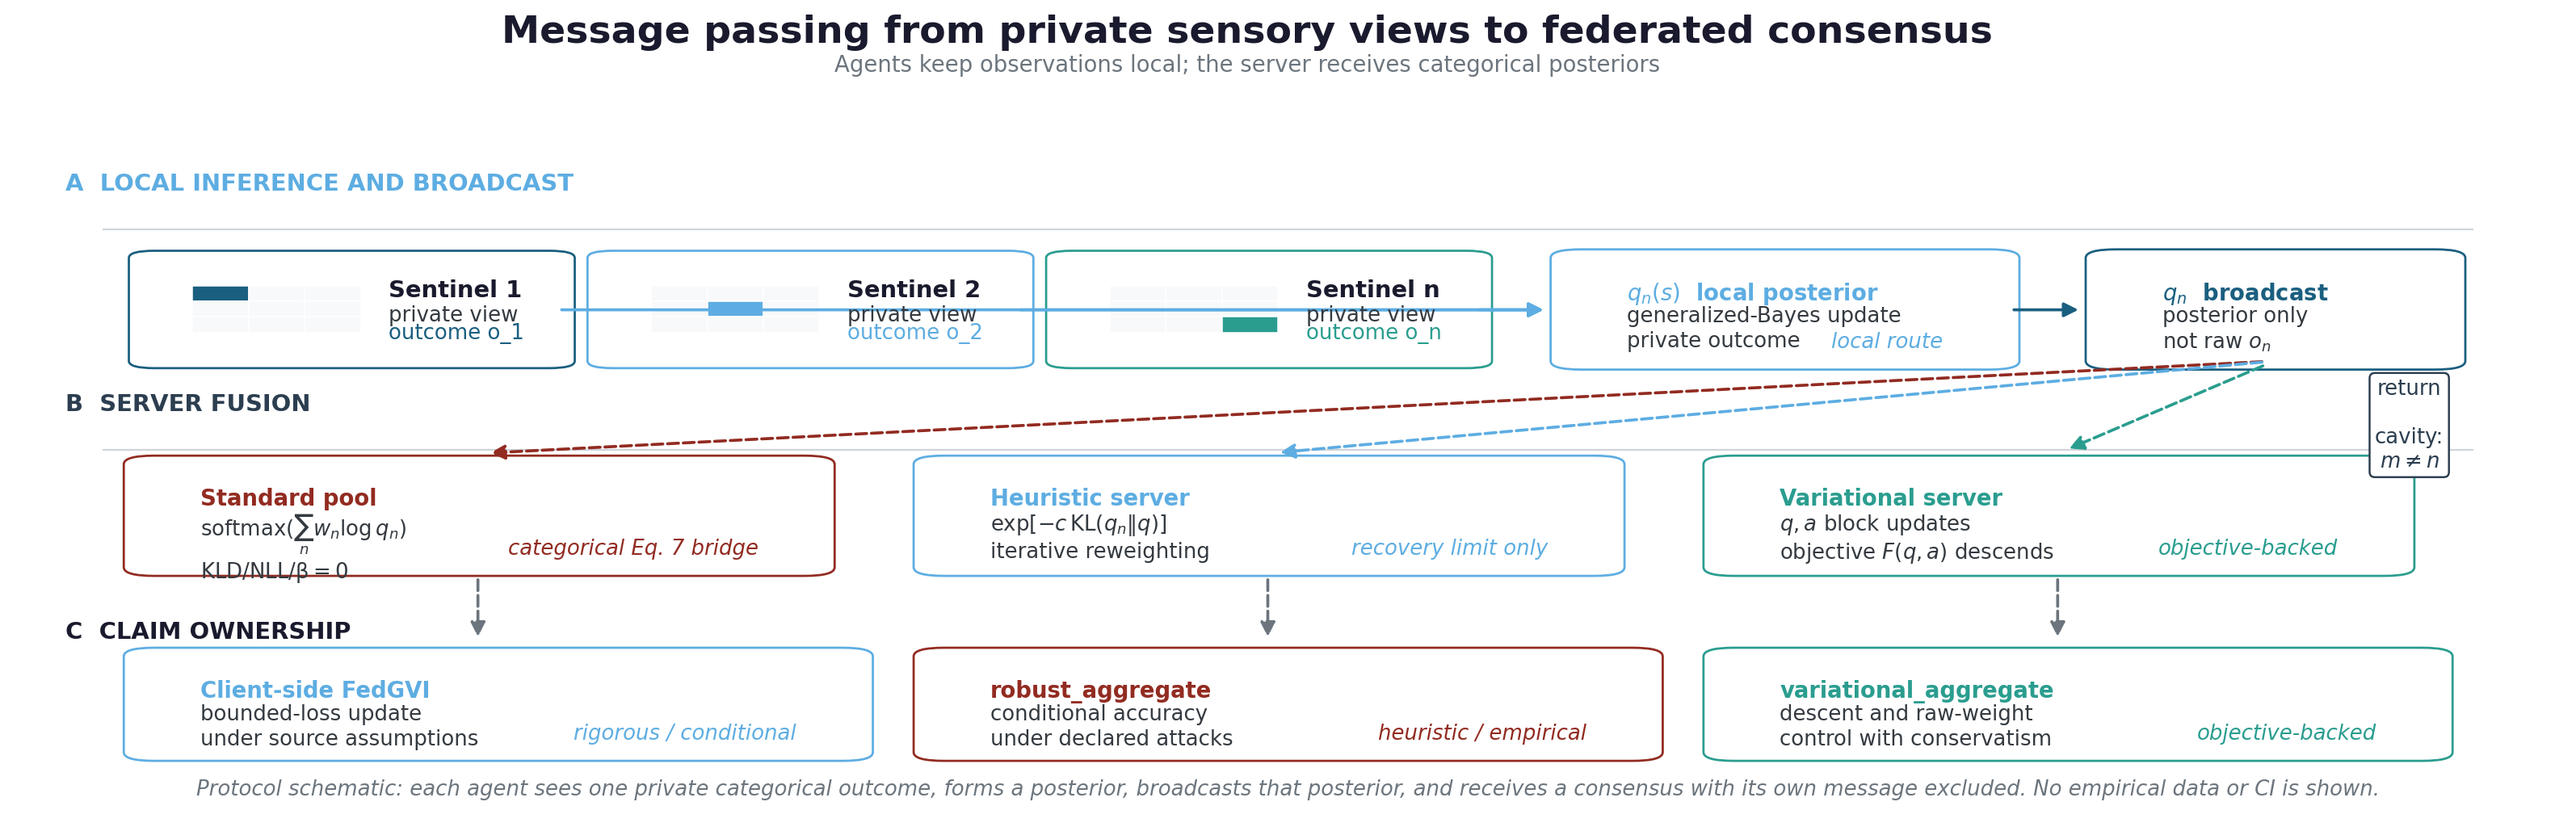
\includegraphics[width=0.95\linewidth,height=0.5\textheight,keepaspectratio,alt={Four-band protocol schematic: agents update from private observations, broadcast local categorical posteriors, enter one of three standard, heuristic, or variational fusion routes, and receive cavity-excluded posteriors. Route-specific badges keep client and server claim owners separate.}]{../figures/message_passing.png}
\caption{Message-passing schematic for Active Fedference. Source
relation: source-inspired original schematic related to Friston et
al.~(2024), Eq. 7 and Fig. 5; estimand: protocol stages and claim
ownership; uncertainty: none. Read the four numbered bands from top to
bottom. The y-axis rows order execution from Stage 1 through Stage 4;
the x-axis is not quantitative and separates the three parallel fusion
routes within Stage 3. Stage 1 begins with private categorical
observations, applies the local update, and keeps NLL/KLD recovery and
robust client-loss claims at the client. Stage 2 transports categorical
posteriors \(q_n(s)\) in the unchanged protocol-v1 envelope rather than
raw outcomes. Stage 3 routes the same broadcasts through the standard
log-linear pool, the server-side \protect\breaktt{robust\_aggregate}
heuristic, or objective-backed \protect\breaktt{variational\_aggregate};
distinct boxes, dashed arrows, and claim-owner badges identify each
route without relying on color. Stage 4 returns a recipient-specific,
cavity-excluded posterior, so an agent does not hear its own message.
The standard route combines the client KL/NLL/\(\beta=0\) recovery with
only the qualified categorical Eq. 7 message-combination specialization,
while the heuristic retains recovery-limit status and conditional
evidence only; no client guarantee migrates to either server rule. This
deterministic formal schematic has no empirical curve, interval, sample
size, or replication unit and does not reconstruct the complete source
protocol.}\label{fig:message-passing}
\end{figure}

\begin{theorem}[Categorical combination and recovery]\label{thm:belief-sharing-recovery}
For finite $\mathcal S$ and $q_n(s)>0$, take Eq. 7 inputs
$m_n(s)=\log q_n(s)+kappa_n$, with state-constant $kappa_n$ and fixed $w_n$.
$\operatorname{softmax}(\sum_n w_n m_n)$ equals
(\ref{eq:log-linear-pool}). At $c=0$, the server returns it by
(\ref{eq:robust-identity}). This identifies categorical combination and
recovery only, not the protocol or $c>0$ behavior.
\end{theorem}

At \(c=0\), every reweighting multiplier is \(\exp(0)=1\), the iteration
is skipped, and the same pool code path returns.

\begin{corollary}[Closed-form Bayes recovery]\label{cor:closed-form-bayes}
With KL/NLL, the posterior of (\ref{eq:gen-bayes}) is the prior-times-likelihood
product in (\ref{eq:standard-bayes}). Thus
\breaktt{generalized\_posterior(KLD, NLL)} reproduces Bayes. Under Theorem
\ref{thm:belief-sharing-recovery}, pooling those posteriors specializes Eq. 7's
categorical combination term, not its complete protocol.
\end{corollary}

\begin{equation}\protect\phantomsection\label{eq:standard-bayes}{
q^\ast(s) \;\propto\; \pi_0(s)\,\textstyle\prod_i p(o_i\mid s),
}\end{equation}

Pooling gives the project log-linear pool of
eq.~\ref{eq:log-linear-pool}.

The largest observed discrepancy between
\breaktt{robust\_aggregate(robustness=0)} and \texttt{log\_linear\_pool}
is 0 --- bit-identical, since the zero-robustness branch runs the same
code path --- and between \breaktt{generalized\_posterior(KLD,\ NLL)} and
the analytic Bayes posterior is 5.55e-17, exact to machine precision
(about one ULP); both are reported in sec.~\ref{sec:results-recovery},
so eq.~\ref{eq:robust-identity} and eq.~\ref{eq:standard-bayes} are
verified identities rather than approximations.

The honesty contract binds at exactly this point. The recovery theorem
and its corollary cover only the recovery identity and the per-agent
rigorous axis of sec.~\ref{sec:method-losses}; no statement \emph{about
\breaktt{robust\_aggregate}} transfers a bounded-influence guarantee to
that divergence-reweighting, whose positive property is the
\(\texttt{robustness}=0\) limit of eq.~\ref{eq:robust-identity}.

A scoped no-go rejects a declared separable objective class without
supplying a broader objective certificate. The per-agent influence
weights that the heuristic produces under contamination are
\emph{illustrated}, not guaranteed, in fig.~\ref{fig:robust-weights}.
The separate fig.~\ref{fig:bnn-robustness} is an exploratory
generalized-Bayes point-estimate logistic-regression baseline comparing
joint NLL/L2 and RCCE/L2 configurations. Because both loss and shrinkage
differ, it does not isolate an RCCE-only effect or test the genuine
per-client FedGVI property, which remains source-conditional in
sec.~\ref{sec:method-losses}.

The next subsection closes this exact gap on the server side with a
\emph{different}, objective-backed aggregator.

\subsubsection{Variational aggregation with objective-backed weight
control}\label{sec:method-variational}

The related server construction becomes a genuinely variational rule by
replacing the heuristic's reverse-KL weight update with a forward
cross-entropy update. For \(c>0\) and \(\lambda>0\), treat the consensus
\(q\) and a vector of effective weights \(a = (a_n)\) as joint
variational parameters and define the \textbf{aggregation free energy}

\begin{equation}\protect\phantomsection\label{eq:agg-free-energy}{
\begin{aligned}
F_\lambda(q, a)
&= \sum_n a_n\,\mathrm{CE}(q, q_n) - \lambda H(q)\\
&\quad + \tfrac{1}{c}\,\mathrm{KL_{gen}}(a \,\|\, w).
\end{aligned}
}\end{equation}

where \(\mathrm{CE}(q, q_n) = -\sum_i q_i \log q_{n,i}\) is the
cross-entropy of the consensus relative to agent \(n\), \(H(q)\) is the
consensus entropy, \(c\) is the robustness, and \(\lambda>0\) is the
\texttt{entropy\_weight} coefficient (default \(\lambda=1.0\));
\(\mathrm{KL_{gen}}(a \,\|\, w) = \sum_n [a_n \log(a_n/w_n) - a_n + w_n]\)
is the generalized KL between the effective and base weights.

Each block of \(F_\lambda\) has a closed-form minimizer, so alternating

\begin{equation}\protect\phantomsection\label{eq:agg-updates}{
\begin{aligned}
q
&\leftarrow \mathrm{softmax}\!\Big(
  \tfrac{1}{\lambda}\textstyle\sum_n a_n \log q_n\Big),\\
a_n
&\leftarrow w_n\,\exp\!\big(-c\,\mathrm{CE}(q, q_n)\big).
\end{aligned}
}\end{equation}

is exact block-coordinate descent on eq.~\ref{eq:agg-free-energy}
(\breaktt{variational\_aggregate}) for \(c>0\) and \(\lambda>0\).

The implementation defines the \(\lambda\downarrow0\) endpoint
separately as a deterministic tied-argmax rule; \(\lambda=0\) is not
substituted into the objective or its \(q\)-update.

This substitution changes both orientation and scale:
\(\mathrm{CE}(q,q_n)=\mathrm{KL}(q\|q_n)+H(q)\), and its common \(H(q)\)
term scales all raw weights, which changes the entropy of the subsequent
unnormalized weighted log pool.

The paired \(q\)- and \(a\)-updates in eq.~\ref{eq:agg-updates} are
exact block minimizers of the stated objective; that fact does not
derive the reverse-KL heuristic.

Because \(F\) is biconvex, we run the descent \textbf{multi-start}
(pool, uniform, and arithmetic-mean seeds, lowest observed \(F\) among
converged starts; otherwise the lowest unfinished trace is returned with
\texttt{converged=False}) so a near-one-hot adversary is not left at the
product-of-experts seed in the tested contamination regimes --- the
detail that supports the effective-weight diagnostic
(sec.~\ref{sec:supp-variational}).

The full derivation, the formal statement (block descent, \(c\to0\)
recovery, and the raw effective-weight bound), and the numerical
witnesses are in sec.~\ref{sec:supp-variational}; the empirical descent
and influence collapse are shown in fig.~\ref{fig:aggregation-descent}
and fig.~\ref{fig:bounded-influence} and reported in
sec.~\ref{sec:results-variational}.

The authoritative notation supplement records the complete objective
contract in eq.~\ref{eq:notation-variational-objective}.

This upgrades the server side from an untracked heuristic to a derived
generalized-Bayes aggregation with an explicit redescending raw-weight
property: a single confidently-wrong agent earns raw weight
\(a_n = w_n\exp(-c\,\mathrm{CE}(q,q_n)) \le w_n\) that vanishes as it
diverges, whereas the naive pool grants every agent the fixed weight
\(w_n\) however wrong it is.

The trade is conservatism --- the \(-H(q)\) term makes the stationary
point a maximum-entropy-biased consensus consistent with the weighted
cross-entropies, so \breaktt{variational\_aggregate} is deliberately
flatter than the product-of-experts and does \emph{not} maximize peak
point-accuracy. The two server-side rules therefore play complementary,
never-conflated roles, both reported: the sharp
\breaktt{robust\_aggregate} heuristic for accuracy under contamination
(sec.~\ref{sec:results-verdict}) and the conservative
\breaktt{variational\_aggregate} for a server-side objective with stated
weight control (sec.~\ref{sec:results-variational}).

A temperature parameter \(\lambda>0\) (controlled by
\texttt{entropy\_weight}, default \(\lambda = 1.0\)) generalizes the
objective to \(F_\lambda\); lower \(\lambda\) sharpens the variational
\(q\)-block toward a maximizing state for its current weighted log pool.

The tempered family (sec.~\ref{sec:supp-tempered}; objective
eq.~\ref{eq:tempered-family}) recovers the full-entropy variational
aggregator at \(\lambda = 1.0\) and has a separately implemented
deterministic tied-argmax endpoint as \(\lambda\downarrow0\); neither
endpoint is guaranteed accurate and neither is an algebraic recovery of
\breaktt{robust\_aggregate}.

The effective-weight \(a\)-update is unchanged for every \(\lambda>0\),
so the raw-weight bound holds over the objective-defined family.

\subsection{Belief sharing: the standard aggregation
corner}\label{sec:method-belief-sharing}

\breaktt{belief\_sharing.share\_round} lifts the aggregation rule of
sec.~\ref{sec:method-aggregation} to a colony of categorical sentinel
agents.

Each agent has a private sensory outcome and a local posterior over the
same shared latent location; it broadcasts the posterior, not its raw
observation. Following the sensory attenuation that the active-inference
formulation of belief sharing imposes \citep{friston2024federated} ---
``agents do not hear themselves'' --- an agent's heard consensus
excludes its own message:

\begin{equation}\protect\phantomsection\label{eq:belief-round}{
q_{-n} \;=\; \mathrm{normalize}\!\left(q/t_n\right),
}\end{equation}

so the round in eq.~\ref{eq:belief-round} implements the declared
categorical colony-hive-mind mechanism. With the naive fusion rule of
eq.~\ref{eq:log-linear-pool}, eq.~\ref{eq:belief-round} is the project's
standard log-linear-pool consensus.

Under the explicit shared-support, posterior-log-potential, and
fixed-weight assumptions of sec.~\ref{sec:method-aggregation}, it
specializes Eq. 7's message-combination term; it does not reconstruct
the complete source protocol.

With the server-side robust rule it yields a hive-mind that can
down-weight a contaminated sentinel --- an effect the contamination
sweep of sec.~\ref{sec:results-robustness} measures rather than assumes,
and one that carries no guarantee beyond the recovery limit.

The per-round diagnostics --- the post-sharing belief matrix, the global
consensus, and the mean surprise and accuracy against a known
ground-truth state --- are returned by \texttt{share\_round} and drive
Studies 1 and 4.

fig.~\ref{fig:message-passing} makes this concrete: three sentinel cards
begin with different private categorical views of the nine-cell world,
convert those views into local posteriors, and send only those
posteriors to a fusion route. The return path is a cavity message, so
the consensus heard by agent \(n\) excludes the local posterior \(q_n\).

The figure remains a protocol map rather than a new result; the
empirical belief matrix and free-energy comparison remain the evidence
surfaces in fig.~\ref{fig:belief-heatmap} and
fig.~\ref{fig:free-energy}.

Because eq.~\ref{eq:belief-round} calls the aggregation rule of
eq.~\ref{eq:log-linear-pool} or its robust generalization, the recovery
identity of eq.~\ref{eq:robust-identity} propagates upward: a colony
running \texttt{share\_round} at zero server robustness is bit-identical
to a colony running the project's standard log-linear-pool round.

Under the qualified categorical bridge, the pool realizes only the
source message-combination specialization; the robust round is a project
extension, not a reconstruction of the active-inference ensemble
literature \citep{friston2024federated, heins2023collective}.

sec.~\ref{sec:results-belief_sharing} reports that communicating
colonies reach a mean variational free energy of 13.2190 nats against
16.5298 nats for incommunicado colonies across 480 seeds, with the
per-agent belief matrix before and after a round shown in
fig.~\ref{fig:belief-heatmap} and the colony comparison in
fig.~\ref{fig:free-energy}.

The honesty boundary of sec.~\ref{sec:robustness-axes} carries through
the lift unchanged. The robustness that eq.~\ref{eq:belief-round}
inherits when the colony fuses with the server-side heuristic is the
divergence-reweighting device of sec.~\ref{sec:method-aggregation},
whose positive property is the naive-recovery limit and whose declared
separable objective class has a scoped no-go result.

The per-agent FedGVI bounded-influence result enters the colony only
through the rcce/AR client losses of sec.~\ref{sec:method-losses}, under
the source theorem's matching assumptions, applied inside each agent's
local generalized-Bayes update.

The robustness sweep in sec.~\ref{sec:results-robustness} and the
variational supplement in sec.~\ref{sec:supp-variational} keep the three
axes distinct. The federation transport (sec.~\ref{sec:supp-federation})
realizes this sharing over queue-backed worker channels; by Proposition
\ref{prop:federation-bit-identity}, the federation bit-identity result,
the consensus is bit-identical to the in-process call, so the channel
adds no precision loss while leaving multi-machine network transport as
future work.

\subsection{Generative model: categorical states, observations, actions,
and hierarchy}\label{sec:methods-generative-model}

The 9 studies --- including the contaminated-sentinel robustness sweep
(Study 4) --- run on one shared sentinel world (Studies 5--7 use its
moving and hierarchical variants): a discrete sentinel
partially-observable Markov decision process (POMDP) using the
categorical world structure illustrated by Friston et al.
\citeyearpar{friston2024federated}, Figures 1 and 4.

We adopt the discrete-state active-inference formulation that the
community has standardized around --- the categorical \(A/B/C/D_0\)
generative model of da Costa et al. \citeyearpar{dacosta2020active}, the
same object the \texttt{pymdp} \citep{heins2022pymdp} and RxInfer
\citep{bagaev2023rxinfer} toolboxes operate on.

We reimplement it in pure NumPy in \texttt{pomdp.py} so the colony, its
sensors, and its dynamics are exactly the ones the analysis executes.

A colony of sentinels watches a single hidden creature whose location is
the shared latent factor they federate beliefs about.

The structural map in fig.~\ref{fig:generative-model-schema} follows the
same generative-model vocabulary while making the implementation
boundary visible: Panel A shows what one agent actually sees --- one
noisy categorical report over the 9 possible locations --- while Panel B
identifies the \(A/B/C/D_0\) factors that turn that report into a local
posterior.

Temporal depth then describes state, observation, posterior, and control
order; hierarchical depth describes conditioned priors. It is a formal
schematic, not an assertion that every displayed dependency is
simultaneously estimated in every study.

\begin{figure}
\centering
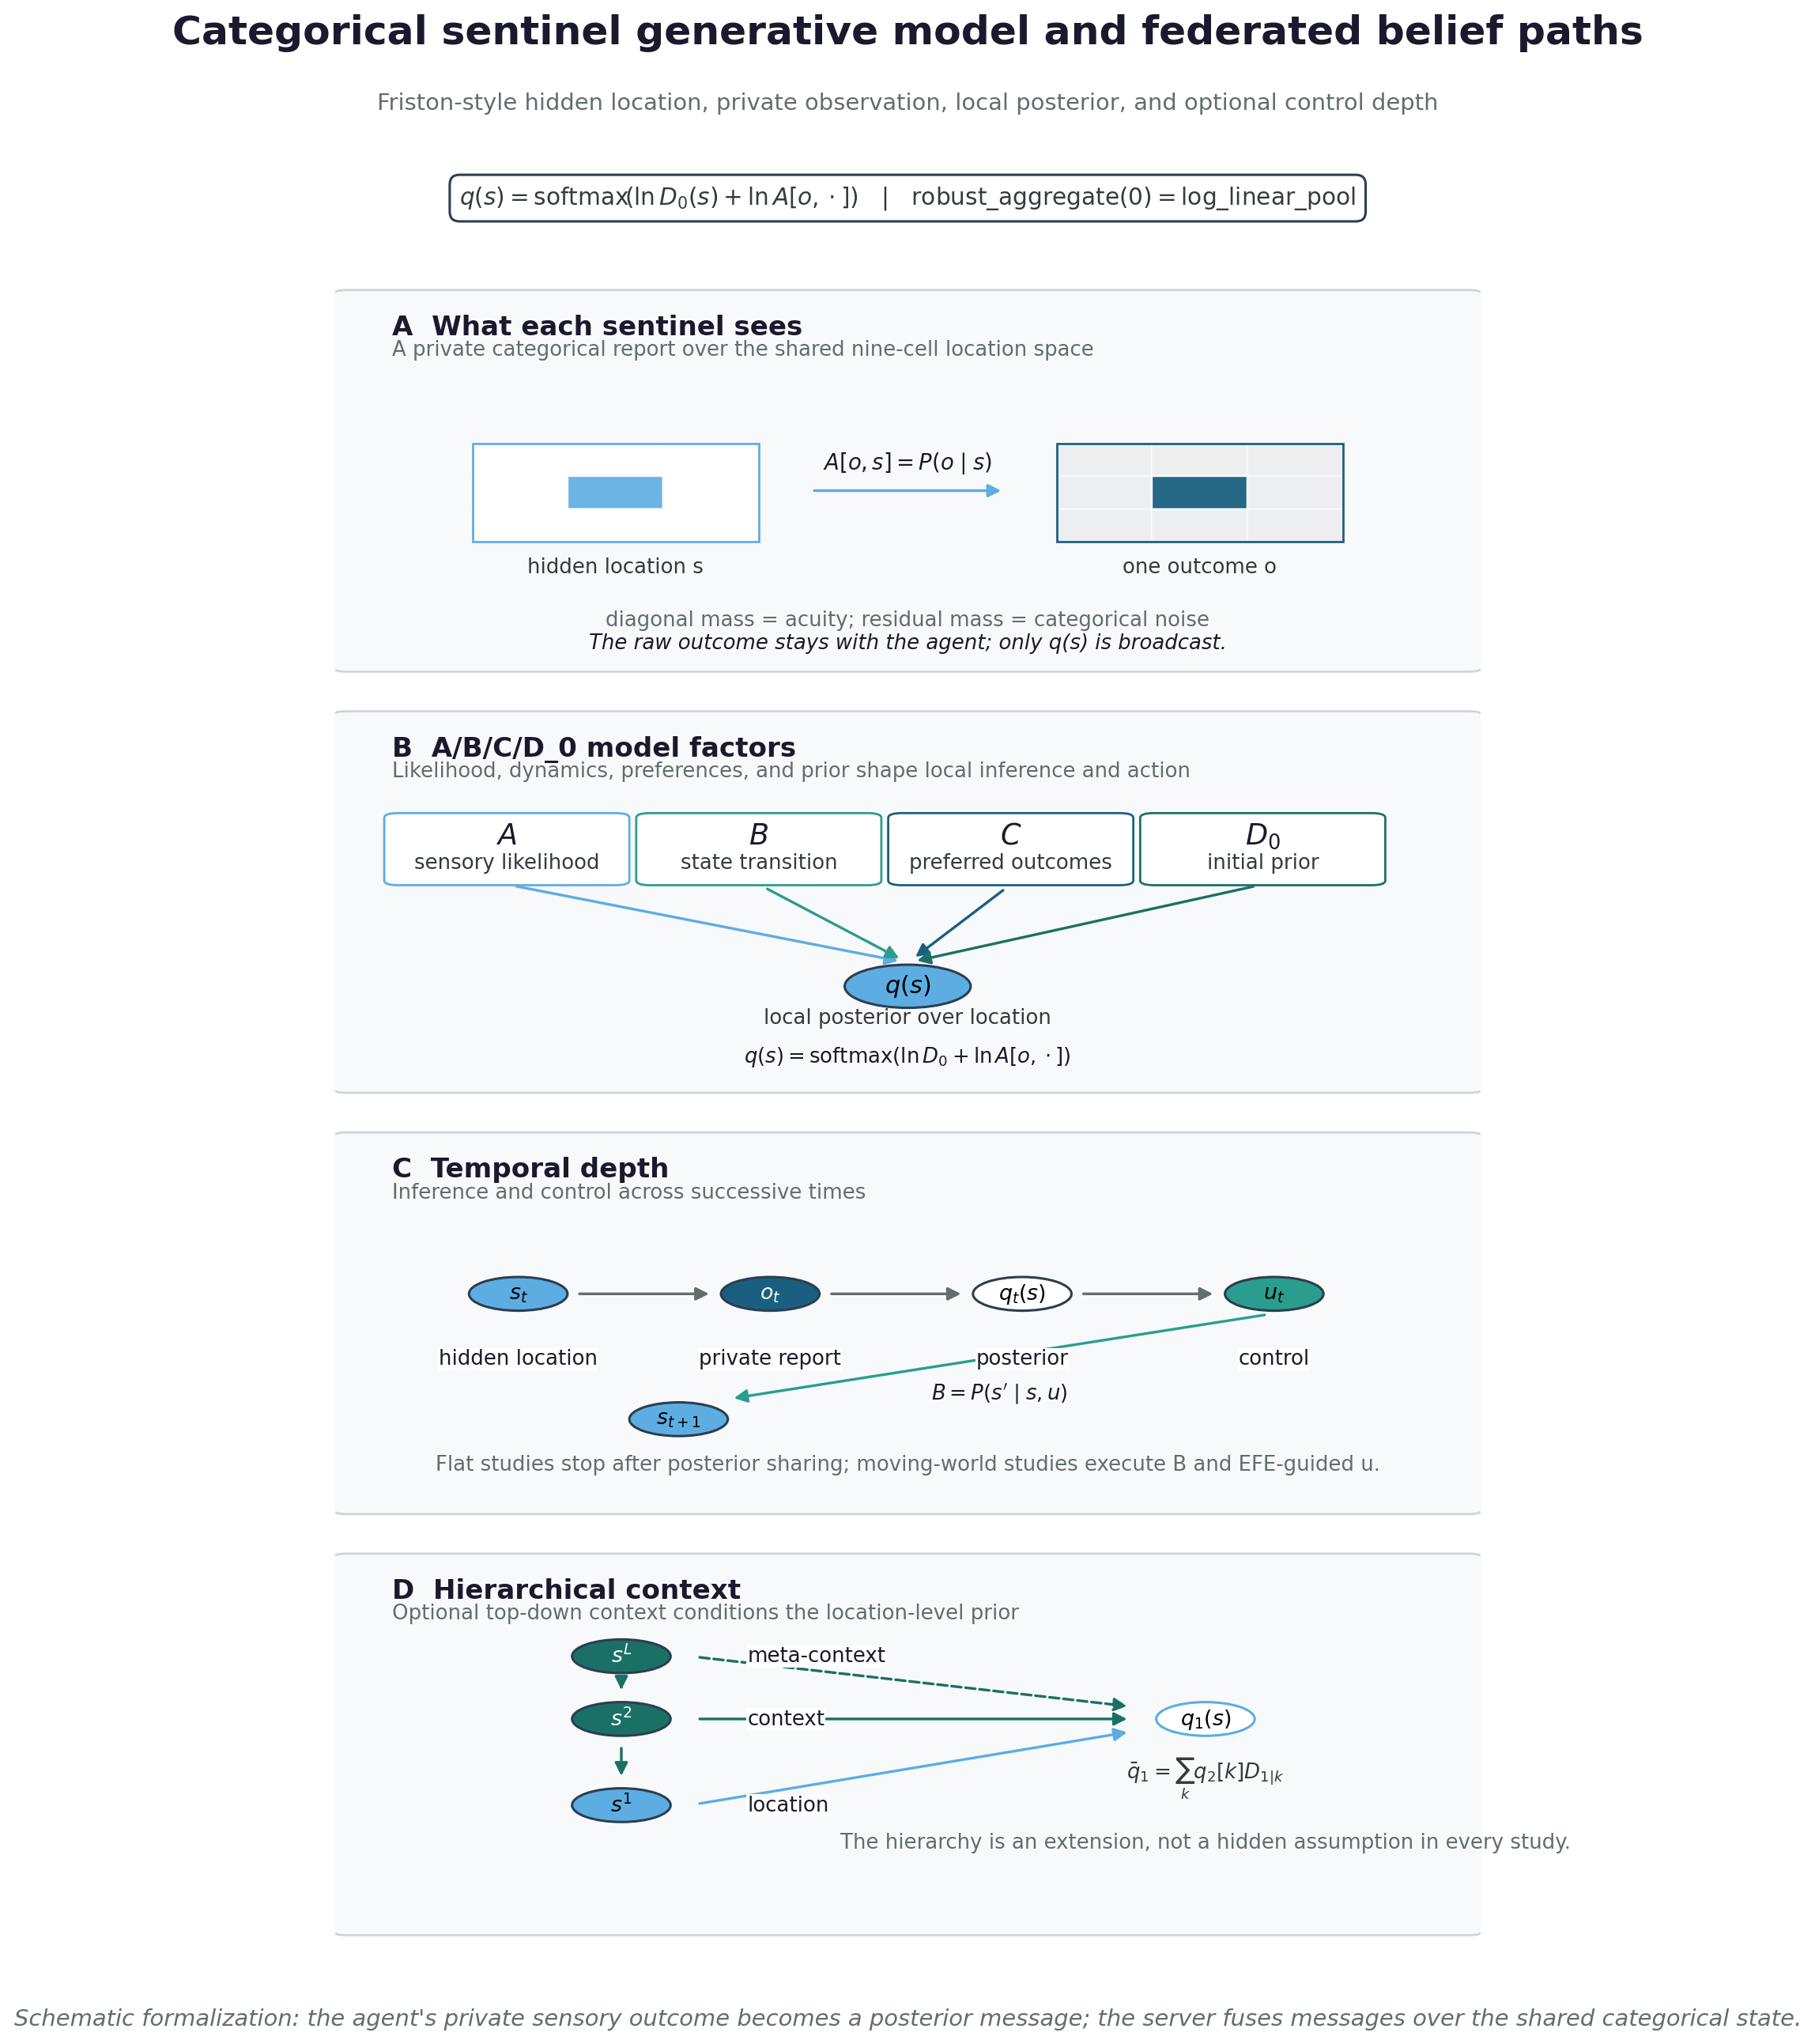
\includegraphics[width=0.95\linewidth,height=0.5\textheight,keepaspectratio,alt={Four-panel categorical generative-model schematic: private observation, A/B/C/D-zero factors feeding a local posterior, temporal state-observation-action order, and optional hierarchical context.}]{../figures/generative_model_schema.png}
\caption{Formal categorical generative-model schema. Source relation:
source-inspired original schematic related to Friston et al.~(2024),
Figs. 1 and 4; estimand: the categorical dependency structure
implemented by the applicable studies. Read Panels A--D from private
sensing, through local factors, to temporal depth and optional
hierarchy. The x-axis is dependency or role order within each panel; the
y-axis positions hidden states, observations, model factors, and context
levels. Panel A maps a hidden 9-cell location through \(A[o,s]\) to one
private categorical outcome. Panel B shows likelihood \(A\), transition
\(B\), preference \(C\), and initial prior \(D_0\) feeding the local
posterior \(q(s)\). Panel C orders state, observation, posterior,
action, and next state; Panel D shows conditioned lower-level priors.
Solid arrows encode implemented categorical dependencies used by the
applicable flat, moving-world, or hierarchical studies; the dashed
upper-context edge marks a qualified optional extension. Direct factor
and node labels, arrow direction, edge style, and panel order duplicate
color. Units are categorical states, outcomes, factors, messages, and
ordered steps. This deterministic formal schematic has no fitted value,
empirical sample, replication unit, error band, or confidence interval;
it does not claim that every source-model component, continuous state,
learning rule, or complete multi-agent protocol has been
reconstructed.}\label{fig:generative-model-schema}
\end{figure}

\subsection{State space: one shared latent
factor}\label{sec:methods-state-space}

The world holds one hidden factor: the creature's location on a square
grid of side \(L\), giving \(n_s = L^2\) location states. Our sentinel
world uses the \(3\times 3\) cardinality illustrated in Friston et al.
\citeyearpar{friston2024federated}, Fig. 1, so \(n_s = 9\) --- the
cardinality \breaktt{pomdp.N\_LOCATIONS} exposes and
\breaktt{experiment\_config} carries as \texttt{n\_locations}.

This single location factor is precisely the latent the colony gossips
about: it is the shared argument of the log-linear pool
(eq.~\ref{eq:log-linear-pool}) and of every belief-sharing round
(eq.~\ref{eq:belief-round}). Fixing one hidden factor keeps the recovery
limits of sec.~\ref{sec:formalism} closed-form and exactly testable,
rather than approximated.

\subsection{Four categorical tensors: likelihood, transitions,
preferences, priors}\label{sec:methods-abcd}

The generative model is the tuple \((A, B, C, D_0)\) in the discrete
active-inference convention: a categorical probability mass function is
a non-negative vector summing to one, and a likelihood matrix is shape
\((n_o, n_s)\) whose columns (indexed by hidden state) are categorical.

\textbf{Observation likelihood \(A = P(o\mid s)\).} Each sentinel
observes the creature's cell through a noisy sensor. With probability
\texttt{acuity} the sensor reports the true cell; the residual mass
\(1-\text{acuity}\) spreads uniformly over the other \(n_s-1\) cells.
With outcome cardinality \(n_o = n_s\), the single location modality is
one \((n_s, n_s)\) matrix:

\begin{equation}\protect\phantomsection\label{eq:observation-likelihood}{
\begin{aligned}
A_{o s} &= \text{acuity}
&& \text{if }o=s,\\
A_{o s} &= \frac{1-\text{acuity}}{n_s-1}
&& \text{if }o\neq s,\\
\sum_o A_{o s} &= 1.
\end{aligned}
}\end{equation}

The acuity in eq.~\ref{eq:observation-likelihood} tunes how peaked the
sensor is: high acuity gives a near-diagonal \(A\) that pins the
creature; the belief-sharing study deliberately runs the colony at the
low acuity \(\text{acuity} = 0.55\), where no single sentinel can
resolve the location alone and the colony must pool evidence to do so.

When a seeded generator is supplied, each sentinel's acuity is jittered
by a small non-negative perturbation, so a colony carries slightly
heterogeneous likelihoods while every column remains a proper pmf.

\textbf{Transition tensor \(B = P(s'\mid s, u)\).} The creature moves on
the grid under three control paths --- \texttt{still}, \texttt{left},
\texttt{right} --- so \(B\) has shape \((n_s, n_s, n_u)\) with
\(n_u = 3\). \texttt{still} is the deterministic self-loop;
\texttt{left} and \texttt{right} decrement and increment the grid
column, saturating at the walls (a wall-adjacent move in the wall's
direction is a self-loop).

All three controls act on the column index alone, so the creature's row
is preserved and its motion is confined to the horizontal axis of the
grid --- a deliberate one-dimensional control over the two-dimensional
location factor. Every slice \(B_{\cdot\,\cdot\,u}\) is
column-normalized by construction, so the transition is a valid
categorical for each action.

\textbf{Log-preference \(C\).} The sentinel prefers to \emph{see} the
creature near the den (the center cell), encoded as a log-preference
vector of shape \((n_o, 1)\) with a positive bump on the center outcome
and zero elsewhere. The preferred-outcome distribution that the
expected-free-energy decomposition of sec.~\ref{sec:methods-learning}
uses is \(p_C(o) = \mathrm{softmax}(C)[o]\).

\textbf{Initial prior \(D_0\).} The creature is believed to start at the
grid center, so \(D_0\) of shape \((n_s, 1)\) places unit mass on the
center cell. \(D_0\) enters state inference as the log-prior of the
one-step variational update (eq.~\ref{eq:state-inference} below).

The columns-are-pmfs invariant is not assumed --- it is pinned by
ISC-15, which checks that every column of \(A\) and of each
\(B_{\cdot\,\cdot\,u}\) sums to one.

\subsection{One-step variational state inference in the grid
world}\label{sec:methods-state-inference}

Given an observation \(o\), a sentinel forms a posterior over the
creature's location by a single softmax step (Friston et al.
\citeyearpar{friston2024federated}, Eq. 4): the log-prior plus the
additive log-likelihood message, summed over any conditionally
independent modalities \(m\),

\begin{equation}\protect\phantomsection\label{eq:state-inference}{
q(s)
= \mathrm{softmax}\!\left(
\begin{aligned}
&\ln D_0(s)\\
&\quad + \textstyle\sum_m \ln A_m[o_m, s]
\end{aligned}
\right).
}\end{equation}

The message \(\ln A_m[o_m, \cdot]\) is the row of \(A_m\) that the
observed outcome selects; summing messages over modalities makes each
modality an additive evidence term --- the categorical
product-of-experts. The companion variational free energy, the scalar
eq.~\ref{eq:state-inference} minimizes, is

\begin{equation}\protect\phantomsection\label{eq:variational-free-energy}{
\begin{aligned}
F[q]
&= \mathbb{E}_q\!\left[
\begin{aligned}
&\ln q(s) - \ln D_0(s)\\
&\quad - \textstyle\sum_m \ln A_m[o_m, s]
\end{aligned}
\right]\\
&= \mathrm{KL}\big(q \,\|\, D_0\big)
   - \mathbb{E}_q\!\big[\textstyle\sum_m \ln A_m[o_m, s]\big].
\end{aligned}
}\end{equation}

reported in nats. The one-step posterior of eq.~\ref{eq:state-inference}
is its unique minimizer, where \(F\) equals the negative log model
evidence.

Both live in \breaktt{belief\_updating.infer\_states} and
\breaktt{belief\_updating.vfe}, and the free energy of
eq.~\ref{eq:variational-free-energy} is the quantity the
communicating-versus-incommunicado colony comparison of
sec.~\ref{sec:methods-experimental-design} scores.

This inference step is not a separate mechanism bolted onto the colony:
it is the \(L=\mathrm{NLL}\), learning-rate-1 special case of the
generalized-Bayes posterior eq.~\ref{eq:gen-bayes}, reusing the same
locked softmax.

That client identity recovers the stated categorical Bayes substrate at
its trusting limits. The separate server identity in
sec.~\ref{sec:method-aggregation} then yields the project log-linear
pool under its qualified Eq. 7 message-combination bridge; together
these do not recover the complete Friston protocol
(sec.~\ref{sec:formalism}).

\subsection{Hidden-state to action loop: the POMDP
substrate}\label{sec:methods-pomdp-loop}

The categorical POMDP loop in fig.~\ref{fig:pomdp-loop} separates the
common latent-state substrate from the federation transport. In the
sentinel interpretation, an agent is a location-sensitive observer: the
hidden state is one of 9 cells, the private outcome is a noisy
categorical report of that location, and the agent sends its posterior
over the location rather than the report itself.

The flat belief-sharing studies use the observation, posterior, and
communication subset; the moving-world extension also executes
transition and EFE-guided action paths.

The diagram therefore gives readers the active-inference context without
turning a conceptual loop into a claim that every study estimates every
latent or policy quantity.

\begin{figure}
\centering
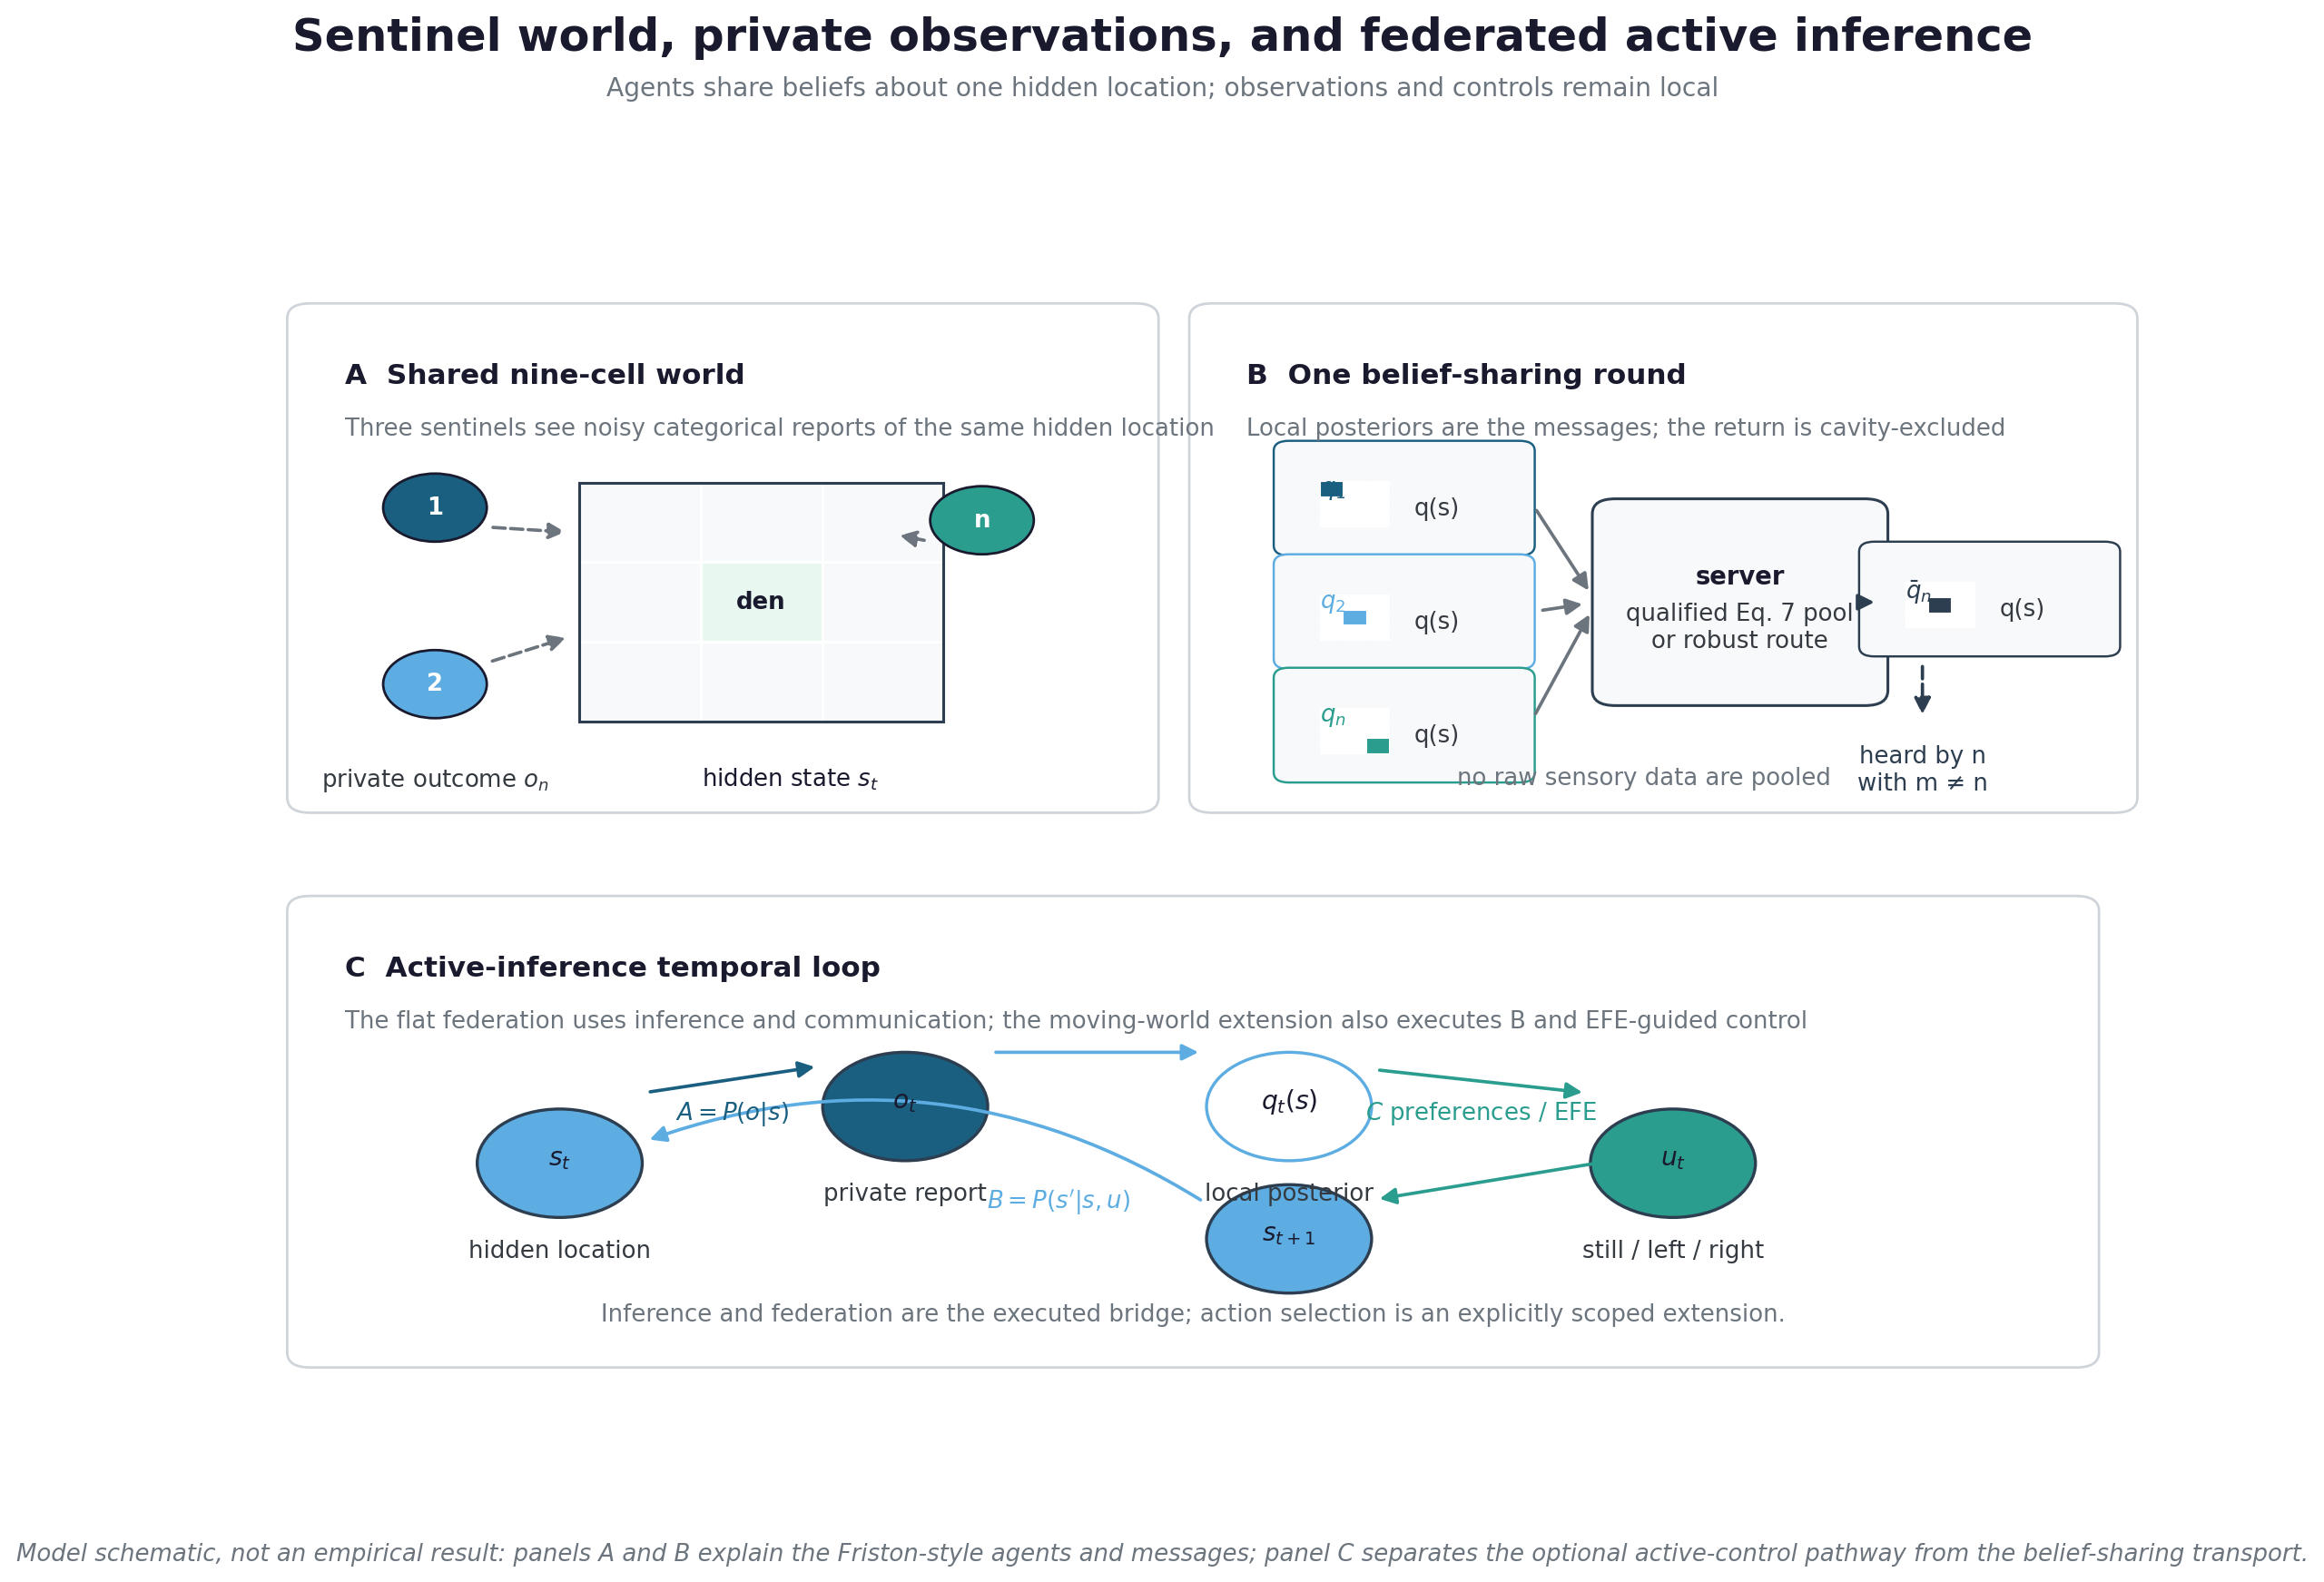
\includegraphics[width=0.95\linewidth,height=0.5\textheight,keepaspectratio,alt={Three-panel active-inference schematic showing a shared hidden world, one cavity-excluded belief-sharing round, and the temporal hidden-state, observation, posterior, action, and transition loop.}]{../figures/pomdp_loop.png}
\caption{Sentinel-world and active-inference loop. Source relation:
source-inspired original schematic related to Friston et al.~(2024),
Figs. 1 and 4; estimand: the implemented POMDP message-and-action
sequence. Read Panels A--C from the shared hidden world, through one
recipient-specific sharing round, to the temporal loop. The x-axis is
the Panel C sequence from hidden state through private observation,
local posterior, action, and next state; the y-axis separates world,
federation, and temporal stages. Panel A shows three agents receiving
private noisy outcomes from one 9-cell hidden world. Dashed sensing
connectors distinguish those private observation relations from the
shared state. Panel B sends only local posteriors along solid arrows to
the qualified Eq. 7 pool or robust route and returns a cavity-excluded
posterior; its dashed recipient connector marks the \(m\neq n\)
exclusion qualification. Panel C uses solid directed arrows for
likelihood update, posterior formation, EFE-guided action, and
transition, with direct \(A\), \(B\), and \(C\) labels. The flat studies
execute inference and sharing; the moving-world extension additionally
executes transition and control. Units are categorical states, outcomes,
posterior messages, actions, and ordered steps. This deterministic
schematic has no fitted effect, replication unit, error band, or
confidence interval; it does not demonstrate a complete source protocol,
physical multi-host federation, Byzantine tolerance, privacy mechanism,
or universally beneficial communication policy.}\label{fig:pomdp-loop}
\end{figure}

\subsection{Learning stack: EFE, Dirichlet updates, and
BMR}\label{sec:methods-learning}

Active-inference agents do more than infer states under a fixed model:
they learn the parameters of the model, score policies by expected free
energy, and revise model structure. The active-inference community has
standardized all three operations
\citep{dacosta2020active, smith2020active}, and Friston et al.
\citeyearpar{friston2024federated} place them at the heart of the
federated belief-sharing scenario.

We reimplement each in closed form so the language-acquisition,
expected-free-energy, and emergence studies of
sec.~\ref{sec:methods-experimental-design} rest on machine-checkable
quantities rather than fitted curves.

\subsection{Conjugate Dirichlet learning from co-occurrence
counts}\label{sec:methods-dirichlet}

A sentinel learns its observation model \(A\) by placing a Dirichlet
prior with concentration \(a\) on each column and updating it
conjugately from observation-state co-occurrence counts (Friston et al.
\citeyearpar{friston2024federated}, their equations 9--12). One learning
step adds the expected sufficient statistics for that step and reads off
the column-normalized posterior mean,

\begin{equation}\protect\phantomsection\label{eq:dirichlet-update}{
a \;\leftarrow\; a + \text{counts},
\qquad
\mathbb{E}[A]_{o s} \;=\; \frac{a_{o s}}{\sum_{o'} a_{o' s}},
}\end{equation}

implemented by \breaktt{learn\_likelihood} in the
\breaktt{dirichlet\_learning} module. Intuitively, each concentration
vector is a running tally of how often each outcome was seen while the
creature occupied a given state: the prior seeds that tally with
pseudo-counts, every step adds the co-occurrences it witnessed, and the
posterior mean is simply the tally renormalized into a categorical.

Likelihood learning is therefore bookkeeping --- accumulate counts, then
normalize --- with no iterative optimization loop.

We drive eq.~\ref{eq:dirichlet-update} with the expected sufficient
statistics under the true model --- a fixed count batch
\(\text{count\_scale}\cdot A^{\star}\) per step, optionally jittered by
a seeded generator. As the concentrations accumulate, the expected
likelihood \(\mathbb{E}[A]\) converges to the data-generating
\(A^{\star}\); convergence is measured by the per-column KL divergence
summed over hidden states,

\begin{equation}\protect\phantomsection\label{eq:dirichlet-kl}{
\begin{aligned}
\mathrm{KL}\big(A^{\star}\|\mathbb{E}[A]\big)
&= \sum_s\sum_o A^{\star}_{os}\\
&\quad\cdot\ln\frac{A^{\star}_{os}}{\mathbb{E}[A]_{os}}.
\end{aligned}
}\end{equation}

which decreases monotonically toward zero --- the standard-Bayes / KL
fixed point. The learned likelihood always has full support (the
Dirichlet prior is strictly positive), so eq.~\ref{eq:dirichlet-kl} is
finite throughout. ISC-17 pins the monotone-decreasing KL trajectory,
and the language-acquisition study of
sec.~\ref{sec:methods-experimental-design} reports the descent of
eq.~\ref{eq:dirichlet-kl} across 24 steps.

The implementation also carries the \(\eta\) forgetting hyperprior of
Friston et al. \citeyearpar{friston2024federated}, their equation 12:
before each conjugate addition the running concentration is decayed so
the \emph{total} concentration mass saturates at \(\eta\) rather than
growing without bound, modeling an agent that stays adaptable instead of
becoming infinitely confident. With \(\eta\) unset the classical
unbounded accumulation of eq.~\ref{eq:dirichlet-update} is recovered.

\subsection{Expected free energy as the action-selection
objective}\label{sec:methods-efe}

A sentinel scores a candidate policy \(\boldsymbol{\pi}\) by its
expected free energy \(G(\boldsymbol{\pi})\), which the active-inference
formulation decomposes two equivalent ways (Friston et al.
\citeyearpar{friston2024federated}, their equation 2): a cost view of
risk plus ambiguity, and a value view of pragmatic plus epistemic value.

The two views are the same scalar rearranged, stated as
eq.~\ref{eq:efe-decomposition} and pinned to a zero residual by the
algebraic identity eq.~\ref{eq:efe-identity} in
sec.~\ref{sec:formalism}.

We compute every term in closed form from the categorical model
\((A, B, C, D_0)\) in \breaktt{expected\_free\_energy.decompose}:

\subsubsection{Risk}\label{risk}

\emph{Risk} is
\(\mathrm{KL}\big(q(o\mid\boldsymbol{\pi})\,\|\,p_C(o)\big)\), the
deviation of the policy-predicted outcomes from the preferred-outcome
pmf \(p_C(o)=\mathrm{softmax}(C)[o]\). Write
\(q_{\boldsymbol{\pi}}(o):=q(o\mid\boldsymbol{\pi})\) for this
scored-policy outcome predictive, used in the remaining terms.

\subsubsection{Ambiguity}\label{ambiguity}

\emph{Ambiguity} is the expected likelihood entropy
\(\mathbb{E}_{q(s)}\!\big[H[p(o\mid s)]\big]\), the outcome uncertainty
given the state.

\subsubsection{Pragmatic value}\label{pragmatic-value}

\emph{Pragmatic value} is the expected log-preference
\(\mathbb{E}_{q_{\boldsymbol{\pi}}(o)}[\ln p_C(o)]\) --- the utility,
exploitation term.

\subsubsection{Epistemic value}\label{epistemic-value}

\emph{Epistemic value} is the state-outcome mutual information
\(H[q_{\boldsymbol{\pi}}(o)] - \mathbb{E}_{q(s)}[H[p(o\mid s)]]\) ---
the expected information gain that drives exploration.

Because there is no sampling, the identity of eq.~\ref{eq:efe-identity}
holds to floating-point tolerance; ISC-19
(\breaktt{expected\_free\_energy}) pins the residual of the decomposition
to zero and pins each term's semantics independently (deterministic
likelihoods give zero ambiguity; uninformative likelihoods give zero
epistemic value; preference-matched predictions lower risk).

fig.~\ref{fig:efe-decomp} visualizes the additive cost view and the
signed pragmatic/epistemic waterfall terminating at
\(G(\boldsymbol{\pi})\) --- a deterministic identity (Proposition
\ref{prop:efe-decomposition}), not a fitted result.

\subsection{Bayesian model reduction for the configured pruning sign
control}\label{sec:methods-bmr}

Sentinels also revise model \emph{structure}. Bayesian model reduction
(BMR) scores whether a reduced model --- for example one that prunes a
redundant location column by shrinking its concentration toward zero ---
has more evidence than the full model, \emph{without re-running
inference} (Friston \& Penny via the post-hoc model optimization lineage
\citep{friston2011post}; the same Beta-function identity is their
equation 13 (Friston et al. \citeyearpar{friston2024federated})).

Because the likelihood is shared, the reduced posterior is available in
closed form,
\(\text{reduced\_post} = \text{post} + \text{reduced\_prior} - \text{prior}\),
and the change in (negative) variational free energy is a difference of
log multivariate Beta functions,

\begin{equation}\protect\phantomsection\label{eq:bmr-deltaf}{
\begin{aligned}
\Delta F
&\;=\; \ln B(\text{prior}) - \ln B(\text{post})\\
&\qquad + \ln B(\text{reduced\_post})\\
&\qquad - \ln B(\text{reduced\_prior}),\\
\ln B(a)
&\;=\; \textstyle\sum_k \ln\Gamma(a_k)
 - \ln\Gamma\!\big(\sum_k a_k\big).
\end{aligned}
}\end{equation}

computed in \breaktt{bayesian\_model\_reduction.reduce}. A positive
\(\Delta F\) in eq.~\ref{eq:bmr-deltaf} means the reduced model carries
more evidence --- the pruned structure was redundant and should be
adopted; a negative \(\Delta F\) means the reduction destroyed support
the data require.

When the reduced prior equals the prior the score is identically zero in
exact algebra, a zero point the suite pins to machine precision
(ISC-20).

The configured BMR sign-control study of
sec.~\ref{sec:methods-experimental-design} uses this operation over
\(n = 4\) candidate states. It contrasts a redundant reduction
(\(\Delta F = 3.68\) nats; adopt) with a supported one
(\(\Delta F = -27.67\) nats; reject) in fig.~\ref{fig:emergence-bmr}.
This fixed-candidate algebraic comparison is deterministic, so it has no
resampled sample or bootstrap interval and does not establish structure
discovery or universal emergence.

\subsection{Contamination models: declared failure modes for belief
fusion}\label{sec:methods-contamination}

Robust belief fusion only earns its keep when some agents are wrong. The
active-inference community has built ensembles that coordinate by
sharing beliefs and observations
\citep{friston2024federated, heins2023collective, albarracin2022epistemic, kaufmann2021collective},
but it has assumed those beliefs are trustworthy in the cited modeled
protocols: fusion is treated as exact-Bayes pooling of well-calibrated
reports.

The robust-Bayes and federated-learning literatures
\citep{mcmahan2017communication, ashman2022partitioned, mildner2025fedgvi}
have, in turn, studied robustness to corrupted clients under their
declared settings, but outside the generative-model-bearing POMDP
setting.

This section defines the corruption process that lets us test fusion
robustness inside the active-inference colony --- the experimental
complement of the robust aggregation rule of
sec.~\ref{sec:method-aggregation}.

\subsection{Corruption process for adversarial belief
broadcasts}\label{sec:methods-corruption}

In the sentinel world a healthy sentinel reports a well-calibrated
categorical over the creature's location; a contaminated one reports
something corrupted. \breaktt{contamination.contaminate} manufactures the
corrupted reports. Every corruption is a convex mixture of the agent's
belief \(b\) with a corruption target \(t\), governed by a single rate
\(r \in [0, 1]\),

\begin{equation}\protect\phantomsection\label{eq:contamination-mix}{
\tilde b \;=\; (1 - r)\, b \;+\; r\, t,
}\end{equation}

so the experiments sweep exactly one knob. The convex form of
eq.~\ref{eq:contamination-mix} gives a clean limit and is the anchor of
the suite (ISC-26): at \(r = 0\) every corruption kind returns the input
belief unchanged, so contamination is a strict, continuous departure
from the uncorrupted Friston belief-share --- never a discontinuity.

This section defines the three core corruption targets \(t\), each
capturing a distinct failure of a federated agent. Geometrically the
three are three landmarks of the probability simplex --- a wrong vertex
(\texttt{confident\_wrong}), the flat centroid (\texttt{uniform}), and a
random interior point (\texttt{label\_noise}) --- so the mixture of
eq.~\ref{eq:contamination-mix} drags an honest belief toward a
qualitatively different destination in each case.

Two further mechanisms (\texttt{byzantine} and \texttt{drift}) extend
the same convex-mix contract and are introduced in the extended-methods
supplement (sec.~\ref{sec:supp-contamination}).

\textbf{\texttt{confident\_wrong} --- the adversarial sentinel.} This is
the lookout that points to one wrong cell and insists on it with total
certainty. The target is a one-hot spike on a wrong state,
\(t = \mathrm{onehot}(s_{\text{wrong}})\), so \(\tilde b\) is mixed
toward a confident, mistaken delta.

Callers choose \(s_{\text{wrong}}\) explicitly; the verdict sweep of
sec.~\ref{sec:methods-experimental-design} fixes it once per colony as
the state diametrically opposite the true state on the location grid,
held constant across the entire rate sweep, rather than deriving it from
the agent's current belief.

At \(r = 1\) this is a pure delta on the wrong cell. This is the
saboteur that is \emph{sure} and \emph{mistaken}: exactly the agent that
robust aggregation must reject.

\textbf{\texttt{label\_noise} --- the miscalibrated sentinel.} This is
the lookout with a scrambled sensor: it is not lying toward any
particular cell, only diluting every honest report with the same fixed
sprinkle of noise. The target is a fixed noisy categorical drawn once
from a \(\mathrm{Dirichlet}(1)\) (a random but valid pmf), modeling a
sentinel whose report is partly random rather than adversarial.

Because the noisy target is drawn once and then held fixed across the
rate sweep, the corruption has no direction to exploit and no single
cell to veto --- the robust pool meets diffuse degradation, not a
targeted attack.

\textbf{\texttt{uniform} --- the apathetic sentinel.} This is the
lookout that shrugs: it has lost track of the creature and calls every
cell equally likely. The target is the maximum-entropy uniform pmf
\(t = (1/n_s)\mathbf{1}\), modeling a saturated sentinel that has lost
all information. At \(r = 1\) it reports uniform, contributing no
evidence to the pool rather than actively pulling it toward a wrong
cell.

All three share the contract of eq.~\ref{eq:contamination-mix} and
require an explicit seeded generator --- \texttt{label\_noise} uses it
to draw the noisy target --- so every contaminated report is
reproducible. The grid of rates the sweep uses,
\(\{0, 0.225, 0.45, 0.675, 0.9\}\), deliberately stops below the
pure-veto limit \(r = 1\), where a fully-confident wrong delta forces
\emph{every} pooling rule's accuracy to zero and the robust-versus-naive
contrast vanishes.

\subsection{How contamination meets the three robustness
axes}\label{sec:methods-contamination-axes}

The authoritative guarantee taxonomy is sec.~\ref{sec:robustness-axes};
this section only records where the declared corruption enters each
route.

\subsubsection{Client bounded-loss
route}\label{sec:methods-contamination-client}

A corrupted local observation enters the per-agent generalized-Bayes
update of sec.~\ref{sec:method-losses}. FedGVI's bounded-influence
result applies only under the source theorem's matching loss,
divergence, model, and regularity assumptions \citep{mildner2025fedgvi}.

The logistic-regression comparison in fig.~\ref{fig:bnn-robustness} is a
narrower exploratory proxy: it compares RCCE and NLL point-estimate
gradients under two L2 coefficients. Its legacy \texttt{AR} argument
selects the larger coefficient; it does not evaluate Alpha-Rényi
divergence or inherit the source theorem from the observed curve.

\subsubsection{Heuristic server
route}\label{sec:methods-contamination-heuristic-server}

A corrupted posterior broadcast enters \breaktt{robust\_aggregate} at
fusion. Divergence reweighting can assign a smaller effective weight to
a report far from the current consensus, as the finite diagnostics
figs.~\ref{fig:robustness-sweep}, \ref{fig:robust-weights} illustrate.

The rule's positive formal property is the exact \(c=0\) recovery limit
eq.~\ref{eq:robust-identity}, not a client-loss bound, Byzantine
guarantee, or universal robustness theorem.

\subsubsection{Objective-backed variational server
route}\label{sec:methods-contamination-variational-server}

The same corrupted posterior can instead enter
\breaktt{variational\_aggregate}, whose declared free energy,
block-descent property, and effective-weight bound are given in
sec.~\ref{sec:method-variational}. Those properties belong to that
forward-oriented objective and do not certify \breaktt{robust\_aggregate}
or the source client's bounded-loss theorem.

Contamination is therefore a common stressor, not a license to transfer
a guarantee or empirical result between client, heuristic-server, and
variational-server lanes.

\subsection{Experimental design: studies, estimands, determinism, and
power}\label{sec:methods-experimental-design}

The generative model of sec.~\ref{sec:methods-generative-model}, the
learning operators of sec.~\ref{sec:methods-learning}, and the
corruption process of sec.~\ref{sec:methods-contamination} are exercised
by 9 studies, including the contaminated-sentinel robustness sweep
(Study 4).

The shared configuration (seed budget, colony size, contamination rates,
divergences, trial counts, and the statistics settings) is read from
\texttt{experiment:} in
\href{https://github.com/ActiveInferenceInstitute/Active_Fedference/blob/main/manuscript/config.yaml}{manuscript
rendering configuration}; the remaining per-study parameters are tested
code defaults in \breaktt{src/fedference/experiments/}.

No value is hard-coded in the manuscript, and each token below resolves
to the same configuration the code executed.

\subsection{Determinism through fixed seeds and generated
variables}\label{sec:methods-determinism}

All stochastic steps draw from explicitly seeded generators
(\breaktt{np.random.default\_rng}); the global \texttt{np.random} state
is never touched. The single-run studies use the first configured seed
(0), and the across-seed studies enumerate the deterministic seed list
\(0,\ldots,n_{\text{seeds}}-1\).

Re-running with the same seed reproduces every number in the results
bit-for-bit, so the bootstrap confidence intervals and paired-test
p-values of sec.~\ref{sec:methods-statistics} are themselves
deterministic functions of the seed.

The figure layer follows the same provenance rule. Captions are written
to be self-contained, with axes, resampling units, deterministic runs,
truncated axes, and error-band status disclosed in the caption rather
than left to inference
\citep{rougier2014figures, midway2020visualization}. This is why several
results figures state ``single deterministic run'' or ``no error band''
even when the inferential evidence appears in an adjacent table.

\subsection{Study suite and contamination
sweep}\label{sec:methods-studies}

Studies 1--3 implement reduced categorical protocols that are
source-mechanism analogues of the belief-sharing, language-acquisition,
and model-reduction mechanisms discussed by Friston et al.
\citeyearpar{friston2024federated} on the sentinel POMDP; they are not
exact source-protocol figure replications. The sweep adds the FedGVI
robustness contribution \citep{mildner2025fedgvi}.

Unless a study specifies otherwise, the global defaults are
\(n_{\text{seeds}} = 480\) independent seeds and
\(n_{\text{trials}} = 960\) matched trials per condition.

The inventories in
tbls.~\ref{tbl:study-measures}, \ref{tbl:study_params} separate each
study's declared measure from its compact execution parameters so
neither meaning is compressed at presentation scale.

\begin{longtable}[]{@{}
  >{\raggedright\arraybackslash}p{(\linewidth - 2\tabcolsep) * \real{0.5000}}
  >{\raggedright\arraybackslash}p{(\linewidth - 2\tabcolsep) * \real{0.5000}}@{}}
\caption{Study-to-estimand map for the five declared protocols. Studies
1--3 are source-mechanism analogues, Study 4 is the server-robustness
extension, and Study 5 is the moving-world supplement
(sec.~\ref{sec:results-moving}).}\label{tbl:study-measures}\tabularnewline
\toprule\noalign{}
\begin{minipage}[b]{\linewidth}\raggedright
Study
\end{minipage} & \begin{minipage}[b]{\linewidth}\raggedright
Declared measure
\end{minipage} \\
\midrule\noalign{}
\endfirsthead
\toprule\noalign{}
\begin{minipage}[b]{\linewidth}\raggedright
Study
\end{minipage} & \begin{minipage}[b]{\linewidth}\raggedright
Declared measure
\end{minipage} \\
\midrule\noalign{}
\endhead
\bottomrule\noalign{}
\endlastfoot
1 --- Belief sharing & Communicating versus incommunicado colony free
energy \\
2 --- Language acquisition & Dirichlet-learning KL descent
(eq.~\ref{eq:dirichlet-kl}) \\
3 --- Emergence / BMR & Reduced-versus-full model evidence
(eq.~\ref{eq:bmr-deltaf}) \\
4 --- Robustness sweep & Robust versus naive consensus under
contamination \\
5 --- Disjoint-FOV world & Communication necessity with non-overlapping
fields of view \\
\end{longtable}

\begin{longtable}[]{@{}ll@{}}
\caption{Per-study configuration, read from \protect\texttt{experiment:}
in \protect\texttt{config.yaml} and surfaced as manuscript tokens by
\protect\breaktt{src/manuscript\_variables.generate\_variables}. The
samples carried into statistics are the belief-sharing sample
(\(n = 480\) seeds), the language trajectory (25 ordered points over
\(n = 480\) independent seeds), and the paired robustness trials
(\(n = 960\) per condition).}\label{tbl:study_params}\tabularnewline
\toprule\noalign{}
Study & Key parameters \\
\midrule\noalign{}
\endfirsthead
\toprule\noalign{}
Study & Key parameters \\
\midrule\noalign{}
\endhead
\bottomrule\noalign{}
\endlastfoot
1 --- Belief sharing & \texttt{n\_agents\ =\ 7};
\texttt{acuity\ =\ 0.55} \\
2 --- Language acquisition & \texttt{num\_steps\ =\ 24} \\
3 --- Emergence / BMR & candidate states \texttt{n\ =\ 4} \\
4 --- Robustness sweep & \texttt{n\_agents\ =\ 7};
\breaktt{n\_contaminated\ =\ 2} \\
5 --- Disjoint-FOV world & \texttt{n\_agents\ =\ 3};
\texttt{fov\_width\ =\ 2} \\
\end{longtable}

\textbf{Study 1 --- belief sharing.} A colony of 7 sentinels at the
deliberately low acuity 0.55 each infer the creature location
(eq.~\ref{eq:state-inference}) and share beliefs through the log-linear
pool (eq.~\ref{eq:log-linear-pool}). We compare a \emph{communicating}
colony against an \emph{incommunicado} one of the same size and seed,
scoring each by the mean variational free energy of
eq.~\ref{eq:variational-free-energy}.

Two protocol details: state inference in this study substitutes a flat
(uniform) prior for \(D\), and each belief's free energy is scored
against the pooled evidence of all agents' observations (the disclosure
carried in sec.~\ref{sec:results-belief_sharing}). The across-seed
sample is \(n = 480\) seeds, one colony-mean free energy per seed
(fig.~\ref{fig:free-energy}, fig.~\ref{fig:belief-heatmap}).

\textbf{Study 2 --- language acquisition.} Each configured seed runs one
sentinel trajectory using the conjugate Dirichlet update
(eq.~\ref{eq:dirichlet-update}) over 24 steps. We record the KL descent
of eq.~\ref{eq:dirichlet-kl} at each ordered step, giving 25 points per
trajectory and \(n =
480\) independent seed trajectories for the pointwise interval in
fig.~\ref{fig:language-kl}.

\textbf{Study 3 --- configured BMR sign control.} A redundant model
reduction and a supported one are scored by the BMR free energy of
eq.~\ref{eq:bmr-deltaf} over \(n = 4\) candidate states
(fig.~\ref{fig:emergence-bmr}). This fixed-posterior comparison tests
the expected signs for two declared prunings; it is not a
structure-discovery experiment.

\textbf{Study 4 --- robustness sweep.} The sweep varies two factors on a
colony of 7 sentinels of which 2 are saboteurs
(\texttt{confident\_wrong}, sec.~\ref{sec:methods-corruption}):

\subsubsection{Contamination rate}\label{contamination-rate}

The contamination rate spans \(\{0, 0.225, 0.45, 0.675, 0.9\}\) and is
the convex-mix weight of eq.~\ref{eq:contamination-mix} toward the
confident-wrong delta.

\subsubsection{Server robustness
setting}\label{server-robustness-setting}

The server robustness setting is named with FedGVI
client-loss/divergence vocabulary for cross-reference only:
\(\{KLD, RKL, AR, beta, rcce\}\).

\texttt{KLD} is the non-robust Friston / standard-Bayes baseline (server
robustness 0, eq.~\ref{eq:robust-identity}) and serves as the design's
negative control. The recovery identity guarantees that it reproduces
the naive log-linear pool exactly, so every contrast uses the proved
un-robustified server rather than a separately tuned competitor.

The remaining labels \(\{RKL, AR, beta, rcce\}\) each select a fixed
\breaktt{robust\_aggregate} down-weighting constant. The executed mapping
is KLD (c=0.00), RKL (c=1.50), AR (c=1.30), beta (c=1.70), rcce
(c=1.60), defined in \breaktt{fedference.experiments.\_common}.

None of these labels invoke the client-side
\breaktt{generalized\_posterior} update of sec.~\ref{sec:method-genbayes}
or the divergence family of sec.~\ref{sec:method-divergences}. This
sweep exercises only the server-side heuristic axis of
sec.~\ref{sec:robustness-axes} (\breaktt{robust\_aggregate}), never the
client-side source-conditional theorem lane.

The executed per-divergence down-weighting strengths are fixed constants
defined in \breaktt{fedference.experiments.\_common} and recorded in the
run reports.

The headline verdict pairs 960 independent trials at the fixed
contamination rate 0.800 --- heavy contamination that degrades the naive
pool while staying below the pure-veto cliff
(fig.~\ref{fig:robustness-sweep}, fig.~\ref{fig:robust-weights}). Each
trial contributes one matched (naive, robust) accuracy pair, so the
replication unit is the trial and the estimand is the within-trial
accuracy difference at that single rate.

A complementary exploratory point-estimate logistic-regression proxy
compares joint NLL/L2 and RCCE/L2 configurations under flipped-label
contamination (fig.~\ref{fig:bnn-robustness}). Because both loss and
shrinkage change, this is a composite loss-and-L2 contrast rather than
an RCCE-only effect; it represents no weight-space posterior and does
not implement a FedGVI generalized-posterior objective.

\textbf{Study 5 --- disjoint-FOV moving world.} This extension
(sec.~\ref{sec:results-moving}) places 3 agents on a 2-slot disjoint-FOV
track to test the necessity of communication when agents cannot observe
the same positions. Isolated agents are compared against EFE-guided
communicating agents on accuracy across the moving sentinel's
trajectory.

Five structural extension studies (Studies 5--9, Supplementary sections)
build on the same POMDP substrate and are described there: the moving
disjoint-FOV sentinel (sec.~\ref{sec:results-moving}), the 2-level
hierarchical POMDP (sec.~\ref{sec:results-hierarchical}), the
\(N\)-level extension (sec.~\ref{sec:results-3level}), the 2-D
sensitivity sweep (sec.~\ref{sec:results-sensitivity}), and parameter
recovery (sec.~\ref{sec:results-parameter-recovery}).

\subsection{Sample size and prospective statistical
power}\label{sec:methods-power}

The verdict design answers a deliberate question: pair \emph{many}
trials at \emph{one} high contamination rate rather than spread few
trials across the rate curve.

A matched-pairs Wilcoxon test gains power from the number of matched
pairs, so concentrating \(n = 960\) paired trials at the single rate
0.800 gives the test the resolution to detect the robustness effect;
scattering the same budget across 5 rates would dilute every contrast.

The across-seed studies are powered separately, with \(n =
480\) seeds for belief sharing and \(n =
480\) independent seed trajectories for language acquisition.

The 25 ordered learning points are repeated measures within each seed,
not additional independent replicates, so the language interval does not
count time points as samples.

The structural-extension and cross-study summary tier uses \(n = 128\)
independent seeds and \(n = 40\) matched trials per contamination rate
for its robustness row. Trials and clients are nested within a seed and
are reduced before across-seed inference; they are not additional
independent replicates.

The bounded red-team review grid is a separate source-bound analysis
profile. It uses 160 deterministic seed replicates, with 24 trials
nested within each seed and scenario/rate cell, and retains the
registered rates 0, 0.2, 0.4, 0.5, 0.6, 0.7, 0.8, 0.9 across the finite
attack union clean, confident wrong, permutation, byzantine, drift,
label noise, uniform.

Its independent unit is the configured seed within a declared cell;
cells that share design structure are not treated as independent worlds.
Robust operating points, method settings, and rate profiles are fixed
before the review run.

The grid reports selection-free contrasts and keeps clean, uniform,
label-noise, permutation, confident-wrong, Byzantine, and drift controls
visible. Completion of this finite review does not close
server-heuristic characterization, leakage-free calibration,
external-data, or protocol-reconstruction phases.

We do not merely assert adequacy --- we compute the design power implied
by the observed effect.

For the headline robust method (RKL) the observed-effect design power of
the paired Wilcoxon at the run's \(n = 960\), computed at
\(\alpha = 0.05\) against the directional alternative \texttt{greater}
(robust accuracy exceeds naive), is 1.0000.

The power approximation uses the deterministic noncentral-normal
approximation of sec.~\ref{sec:methods-statistics}, deflated by the
Wilcoxon's Pitman asymptotic relative efficiency, so it is approximately
calibrated for the signed-rank test actually run (exact under a
normal-shift alternative; the power computation is one-sided while the
reported p-values are two-sided).

To bound a confirmatory replication, the prospective sample size needed
to reach the target power 0.80 at the observed effect is \(n = 5\)
matched trials --- the explicit sample-size budget a follow-up study
should adopt.

These power quantities characterize the \emph{server-side} aggregation
contrast; per the honesty contract of sec.~\ref{sec:robustness-axes}
they do not certify the per-client \(\beta\)/rcce guarantees, which are
pinned by the locked core (sec.~\ref{sec:formalism}) rather than by
these aggregation-level statistics.

\subsection{Software environment and configuration
fingerprint}\label{sec:methods-software}

The FedGVI core, the POMDP studies, and the logistic-regression baseline
are pure NumPy / SciPy --- no GPU and no network. The deterministic-MLP
neural complement (sec.~\ref{sec:results-baseline}) additionally uses
PyTorch (CPU); the analysis pipeline executes it and emits its numbers
as tokens exactly like every other result when the \texttt{torch}
optional extra is installed, and otherwise records a skipped status with
unavailable-value sentinels instead of silently fabricating neural
results.

Versions and platform --- including the PyTorch version used for the MLP
complement --- are recorded automatically in
sec.~\ref{sec:reproducibility}.

\subsection{Statistical protocol: matched comparisons, intervals, and
bounded claims}\label{sec:methods-statistics}

No ``robust beats naive'' claim is written before a statistical test
produces it (Algorithm Gate I). Among the active-inference sources
reviewed here, belief-fusion outcomes are typically reported as single
illustrative runs; we treat every headline contrast as a paired
hypothesis test with effect-size estimation, multiple-testing deflation,
confidence intervals, and an observed-effect design-power calculation
--- the reporting discipline expected by robust statistics and applied
inference
\citep{huber2009robust, efron1993bootstrap, koehler2009mcse, morris2019simulation, loy2021lmeresampler, nakagawa2007effect, benjamini1995controlling, wasserstein2016asa}.

The protocol lives in \texttt{statistics.py}, sits at the analysis tier
above the locked FedGVI core, and emits every number the results
sections report; nothing is hard-coded (ISC-30).

\subsection{Paired comparison and standardized effect
size}\label{sec:methods-paired}

The headline claim is \emph{paired}: across matched scenarios --- same
seed, same contamination --- does the robust aggregator raise consensus
accuracy over the naive log-linear pool? For the expanded review grid,
the inferential unit is the seed: trials are nested within a seed/cell
and are averaged before seed-level contrasts.

The primary robustness sweep also retains a trial-level paired
diagnostic, but its matched trial replicates are nested within one fixed
seeded world and are not independent worlds. The seed-level review-grid
estimand is therefore the robust-minus-naive accuracy difference after
the declared trial reduction, not a contrast of two independently drawn
group means.

Each configured robust method is retained in every review-grid rate
panel and has its own seed-level contrast, interval, and test; no
pooled-selected curve or pooled-selected inferential member enters that
grid.

The naive comparator is the project's log-linear pool
eq.~\ref{eq:log-linear-pool}. Under the shared-support,
posterior-log-potential, and fixed-weight assumptions of
sec.~\ref{sec:method-aggregation}, it specializes the
message-combination term of Friston et al.'s Eq. 7
\citeyearpar{friston2024federated}, rather than reconstructing the
complete source protocol.

We test it with the matched-pairs Wilcoxon signed-rank test
\citep{wilcoxon1945individual} (\breaktt{statistics.paired\_test},
ISC-28), interpreted under the usual signed-rank conditions: seed-level
paired differences are independent across the declared seed schedule,
while the primary sweep's trial-level diagnostic remains conditional on
its fixed world; the differences are ranked after zero differences are
removed, and the null is a symmetric distribution of paired differences
around zero rather than an equality-of-means claim
\citep{fay2010wilcoxon}.

This is the right comparison for bounded, often non-Gaussian accuracy
deltas, but it is not assumption-free. The test reports the primary
matched-pairs rank-biserial effect
\(r_{\rm rb} = (T^{+} - T^{-})/(T^{+} + T^{-})\). We retain the monotone
secondary transform \(d_{\rm eq}=2r_{\rm rb}/\sqrt{1-r_{\rm rb}^2}\),
labeled a \emph{rank-biserial-derived d-equivalent}, never raw Cohen's
\(d\) and never a replacement for the mean contrast.

When \(r_{\rm rb}\) saturates at \(\pm1\), the transform diverges;
tables print a signed saturation marker rather than a finite
million-scale value. The primary-sweep headline display method RKL has
rank-biserial effect 1.0000, d-equivalent saturated (r=+1) (large), with
the paired mean difference and bootstrap interval reported alongside it.

\subsection{Bootstrap interval estimates}\label{sec:methods-bootstrap}

Every inferential mean --- colony free energy, learning-curve KL,
per-method accuracy, and the robust-minus-naive accuracy difference ---
carries a 95\% percentile-bootstrap confidence interval
\citep{efron1993bootstrap} from \breaktt{statistics.bootstrap\_ci},
resampled from the declared unit. For the review grid, the unit is the
seed after the nested trials have been reduced; for the primary
fixed-world sweep, the interval is explicitly trial-level and
conditional; for single-seed diagnostics, it is descriptive or
trial-level.

The single-colony mechanistic rate table is \(n=1\) per cell and is
descriptive, not an inferential mean; its companion profile uses the
declared nested design. This separation follows simulation-reporting
guidance to declare the estimand and the independent Monte Carlo unit
\citep{morris2019simulation}.

The interval quantifies variation over the declared resampling unit
(seed, recorded step, or matched trial) and is conditional on this
simulation design, not on unmodeled real-world deployment uncertainty or
alternative contamination models. The headline mean robust-minus-naive
accuracy difference is 0.0809 with 95\% CI \([0.0783, 0.0834]\).

At the verdict rate, the naive pool has mean accuracy 0.9021 (95\% CI
\([0.8993, 0.9049]\)).

The headline display method RKL has mean accuracy 0.9829 (95\% CI
\([0.9827, 0.9832]\)).

For every multi-seed summary we also report the Monte Carlo standard
error (\(\mathrm{MCSE} = s/\sqrt{n_{\rm seed}}\)) and an approximate
two-sided minimum detectable effect (MDE) at the configured target
power. These are precision diagnostics over independent seeds, not
claims about sampling a real population.

The MDE uses a normal approximation conditional on the observed
seed-level standard deviation \citep{koehler2009mcse}; it is reported
alongside the non-parametric interval rather than used to replace the
paired test.

\subsection{Multiple-testing deflation by BH-FDR}\label{sec:methods-fdr}

The sweep compares each robust divergence against the naive pool, so an
uncorrected \(p < 0.05\) across the family would manufacture false
discoveries. We control the false-discovery rate with the
Benjamini-Hochberg step-up procedure \citep{benjamini1995controlling}
(\breaktt{statistics.bh\_fdr}, ISC-29) at \(\alpha = 0.05\).

The verdict family owns one robust-versus-naive contrast per robust
method at the predeclared verdict rate; each rate table owns its own
within-method rate family. Families are not pooled across figures or
across the review-grid cells.

The review-grid families retain all configured method contrasts and do
not derive a selected member by pooled mean.

The procedure returns both the rejection mask and the monotone BH
q-values.

BH controls expected false discovery proportion within the stated
family, not the family-wise probability of any false positive; the
manuscript therefore states the family each table uses. The
positive-contrast rule is strict and conjunctive: a method is a
BH-rejected positive contrast \emph{iff} BH rejects its null
\textbf{and} its rank-biserial effect is positive. This is a statistical
decision for the named family, not a unique scientific winner.

The primary-sweep headline display method has raw
\(p = 1.11 \times 10^{-158}\), deflating to BH
\(q = 1.11 \times 10^{-158}\).

\subsection{Prospective power analysis for the verdict
rate}\label{sec:methods-statistics-power}

We report not only \emph{that} the verdict rejected the null but the
observed-effect planning power implied by the run and the number of
pairs a confirmatory run could budget.

The observed-effect design power of the headline paired Wilcoxon at the
primary sweep's matched-trial unit, \(n_{\rm trial} = 960\),
\(\alpha = 0.05\), alternative \texttt{greater}, is 1.0000; the
prospective sample size for the target power 0.80 at the observed effect
is \(n_{\rm trial} = 5\).

The estimator is the deterministic noncentral-normal approximation to
the matched-pairs \(t\)-test, deflated by the Wilcoxon's Pitman
asymptotic relative efficiency \(3/\pi\), so the reported power is
approximately calibrated for the signed-rank test the harness runs (the
deflation is exact under a normal-shift alternative); note the power
computation is directional for planning, while the reported p-values are
two-sided.

This is an observed-effect planning approximation conditional on the
observed effect size, not independent evidence for the result and not a
confirmatory power guarantee.

\subsection{Reporting tables and the honesty
boundary}\label{sec:methods-reporting}

The results sections render six statistics tables straight from these
tokens: the per-rate accuracy sweep (tbl.~\ref{tbl:robustness_sweep}),
the robust-versus-naive verdict (tbl.~\ref{tbl:robustness_verdict}), the
standardized-effect estimates (tbl.~\ref{tbl:verdict-effect-estimates}),
their paired inference and observed-effect planning diagnostics
(tbl.~\ref{tbl:verdict-inference-power}), the per-method accuracy with
bootstrap CIs at the verdict rate (tbl.~\ref{tbl:accuracy-at-verdict}),
and the effect and inference projections of the per-contamination-rate
paired tests
(tbls.~\ref{tbl:paired-by-rate}, \ref{tbl:paired-by-rate-inference}).

Every cell is a generated token, never hand-typed.

The honesty contract binds at exactly this tier. The effect-size, CI,
and power enrichment above decorates the \emph{server-side}
\breaktt{robust\_aggregate} divergence-reweighting contrasts only.

It does not certify the per-client \(\beta\)/rcce generalized-Bayes
(FedGVI) guarantees, which are pinned by the locked core (Proposition
\ref{prop:robust-loss-recovery} of sec.~\ref{sec:formalism}) rather than
by these aggregation-level statistics --- the three robustness axes of
sec.~\ref{sec:robustness-axes} kept distinct.

\subsection{Evidence classes and replication
hierarchy}\label{sec:methods-evidence-map}

The reporting map in fig.~\ref{fig:evidence-replication-map} makes the
reporting rule explicit. Read each numbered row across its six fields:
result and class, estimand and unit, independent unit, nesting,
permitted support, and prohibited support. A formal identity,
conditional server contrast, protocol check, and application receipt
therefore cannot silently exchange evidentiary standing.

The top nesting strip supplies a shared reading grammar. A seed is
independent only where its report declares it so; matched trials,
agents, contamination roles, ordered steps, and posterior states
otherwise remain nested. The three no-transfer boxes keep these
ownership boundaries explicit. The external source-dataset lane stays
open until a frozen design and source-bound confirmatory report exists.
Fourteen rows cover the headline result families and public software
boundaries; exact estimates and intervals remain in their typed reports
and the native-unit cross-study summary
(fig.~\ref{fig:cross-study-summary}).

\begin{figure}
\centering
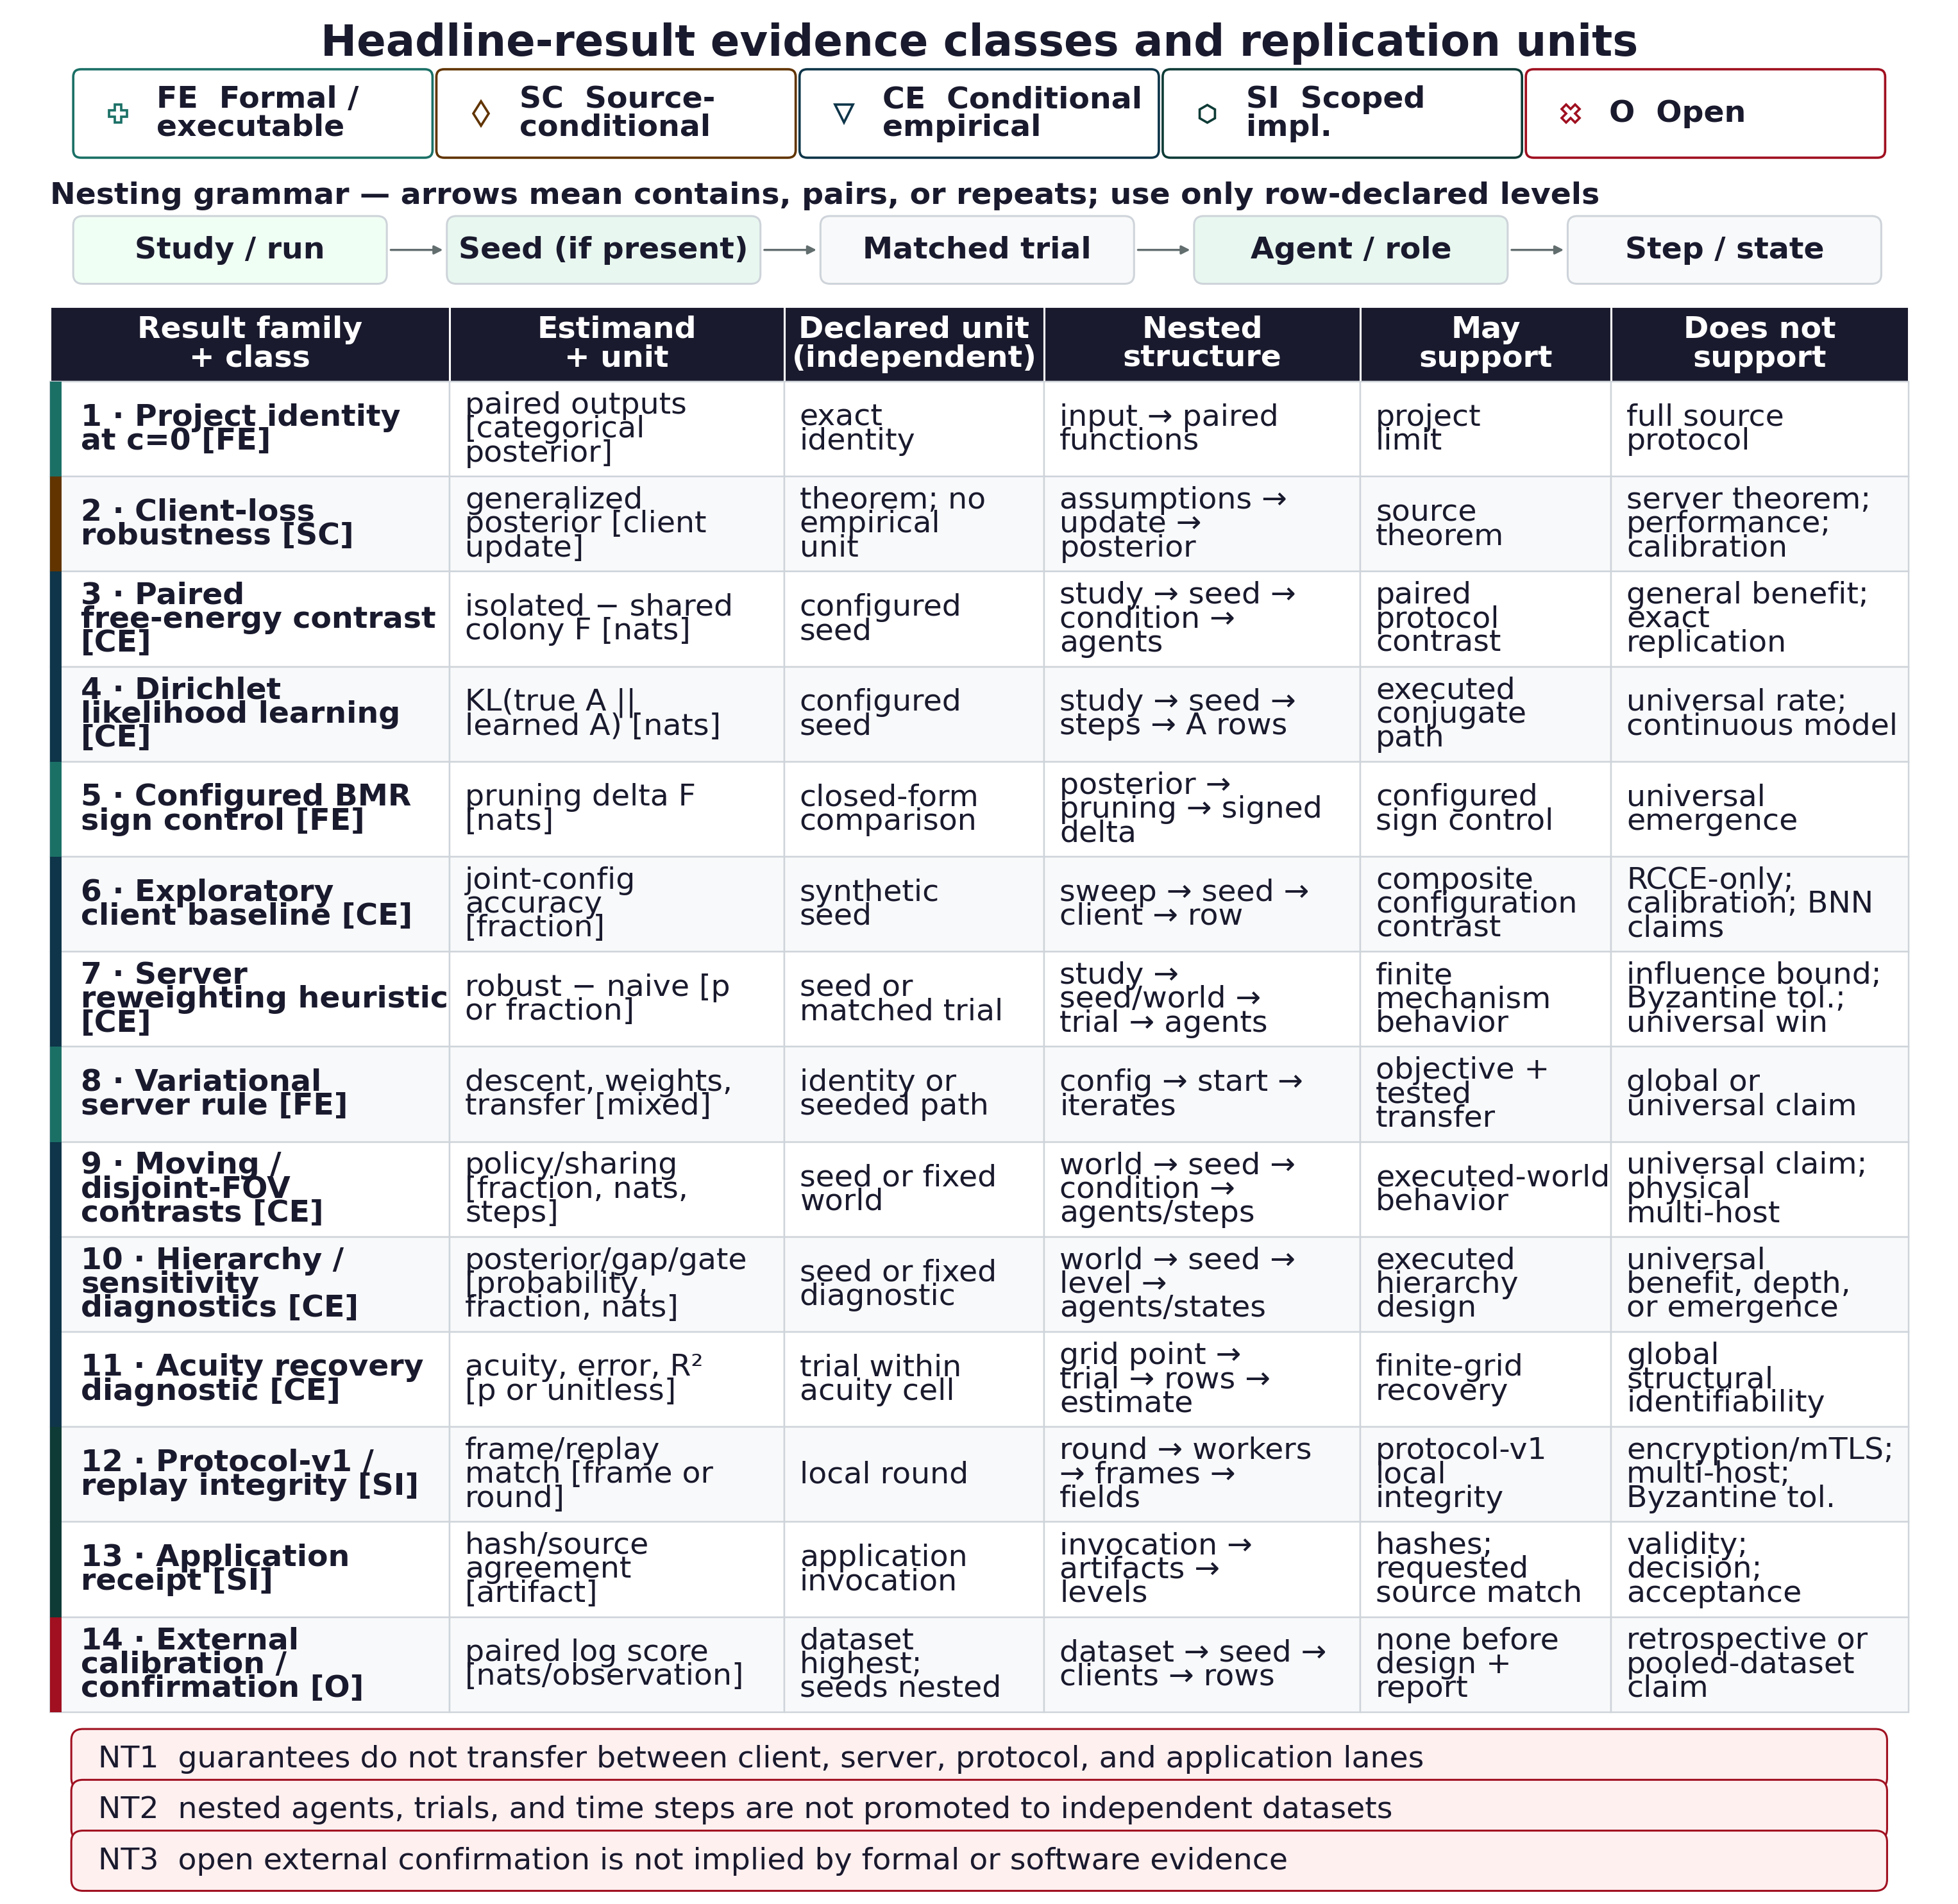
\includegraphics[width=0.98\linewidth,height=0.5\textheight,keepaspectratio,alt={Large-type evidence ledger with fourteen numbered result-family rows and six directly labeled columns. Each row names its class, estimand and unit, replication unit, nesting, permitted support, and prohibited generalization. A five-step nesting strip and three no-transfer boxes keep client, server, study, transport, application, and open confirmation evidence separate.}]{../figures/evidence_replication_map.png}
\caption{Evidence class and replication remain result-family specific;
guarantees do not migrate between client, server, study, protocol, and
application evidence. Source relation: source-owned headline-result and
claim-owner classification; status: deterministic evidence map, not an
empirical result. Fourteen numbered rows align each headline family or
public boundary with six fields: class, estimand and unit, independent
unit, nesting, permitted support, and prohibited support. The rows
retain paired belief-sharing free energy, Dirichlet learning, configured
BMR, moving/disjoint-field worlds, hierarchy/sensitivity, acuity
recovery, and tempered transfer alongside formal, server, protocol,
application, and open-confirmation lanes. A top strip supplies the
generic grammar from study or run through seed when present, matched
trial or condition, agent or contamination role, and ordered step or
posterior state; three bottom boxes state the no-transfer boundaries.
The x-axis indexes six evidence fields; the y-axis indexes fourteen
result families. Class symbols, keylines, row numbers, and direct labels
duplicate color. The estimand and unit are row-specific. No uncertainty
belongs to this deterministic map; underlying intervals resample the
independent unit named on their row while lower levels remain nested.
Exact estimates remain in typed reports and the native-unit cross-study
summary. The figure does not establish source-dataset confirmation,
isolate an RCCE-only effect, transfer a client theorem to a server rule,
promote nested observations to independent datasets, or turn software
integrity into scientific validity.}\label{fig:evidence-replication-map}
\end{figure}

\subsection{Computational complexity and scaling
diagnostic}\label{sec:methods-complexity}

The release now reports computational complexity from the implementation
itself. Let \(N\) be the number of agents, \(S\) the number of
categorical states, \(I\) the solver-iteration budget, \(B\) the number
of variational starts, and \(M\) the number of conditionally independent
observation modalities.

The dominant dense work and the storage actually retained by the current
NumPy paths are summarized separately so neither quantity is compressed
at presentation scale. Here \texttt{LOO} means self-excluding
leave-one-out sharing, and \texttt{server\ round} excludes queue and
network wait.

\textbf{Time, aggregation.} The log, robust, and variational pools have
orders \(\Theta(N S)\), \(\Theta(I N S)\), and \(\Theta(B I N S)\),
respectively.

\textbf{Time, sharing and inference.} Naive LOO, robust LOO, state
inference, and a server round have orders \(\Theta(N^2 S)\),
\(\Theta(I N^2 S)\), \(\Theta(M S)\), and \(\Theta(N log N + I N S)\),
respectively.

\textbf{Storage, aggregation.} The log, robust, and variational pools
retain or peak at \(\Theta(N S)\), \(\Theta(N S + I S)\), and
\(\Theta(N S + I S + B S)\), respectively.

\textbf{Storage, sharing and inference.} Naive LOO, robust LOO, state
inference, and a server round retain or peak at \(\Theta(N S)\),
\(\Theta(N S + I S)\), \(\Theta(S)\), and \(\Theta(N S)\), respectively.

These are dominant interaction counts, not hardware-independent FLOP
totals. The \(N^2\) sharing term is material: with sensory attenuation
enabled, one round computes one global pool and one leave-one-out pool
per agent.

The iterative server rules additionally retain their returned
per-iteration histories, which is why their storage rows include
\(I S\). The server row includes worker-ID sorting and dense
aggregation; incoming serialized belief volume is linear in \(N S\),
while queue and network latency are deliberately outside this
local-compute accounting.

The local path serializes one consensus-plus-weight result; if physical
broadcast bytes are counted per recipient, that outgoing volume
additionally has an \(N^2\) term because each result carries the \(N\)
agent weights.

The accompanying seeded benchmark measures the real public call paths on
the declared grids \(N \in \{4, 8, 16, 32, 64\}\), \(S \in
\{256, 512, 1024, 2048, 4096\}\), self-excluding sharing \(N \in
\{4, 8, 16, 32\}\), and \(M \in
\{1, 2, 4, 8\}\).

The fixed dimensions are \(N=256\), \(S=64\) for aggregation, and
\(S=16384\) for state inference; direct aggregation and server timings
use \(I=6\), while the public robust self-excluding sharing path uses
its solver budget \(I=32\); the default variational path uses \(B=3\).

Each grid point is warmed up \(1\) time(s) and measured \(5\) time(s),
with median time plotted and the observed repeat range shown as a
min--max bar.

The fixed input seed is \(20260728\) on the \(arm64\) machine using
Python \(3.12.12\) and NumPy \(2.4.2\).

The measured log--log slopes are descriptive checks of the expected
orders, not performance guarantees: agent-axis slopes are 0.75
(log-linear), 0.87 (iterative robust), 0.82 (variational), 1.63 (naive
self-excluding sharing), and 1.93 (robust self-excluding sharing);
state-axis slopes are 0.98, 0.97, and 1.01; the modality-axis inference
slope is 0.71.

The slope fit is a timing diagnostic on this machine, not an inferential
test and not evidence that the same constants hold under another BLAS,
accelerator, process topology, or distributed network.

A finite grid can also yield a sublinear fitted slope when validation,
allocation, cache, and interpreter overheads are material; the
implementation-derived order is the governing claim, not equality
between a finite-grid slope and its exponent.

The timing plot in fig.~\ref{fig:complexity-scaling} visualizes the
implementation-derived orders and the corresponding finite-grid timing
diagnostic.

\begin{figure}
\centering
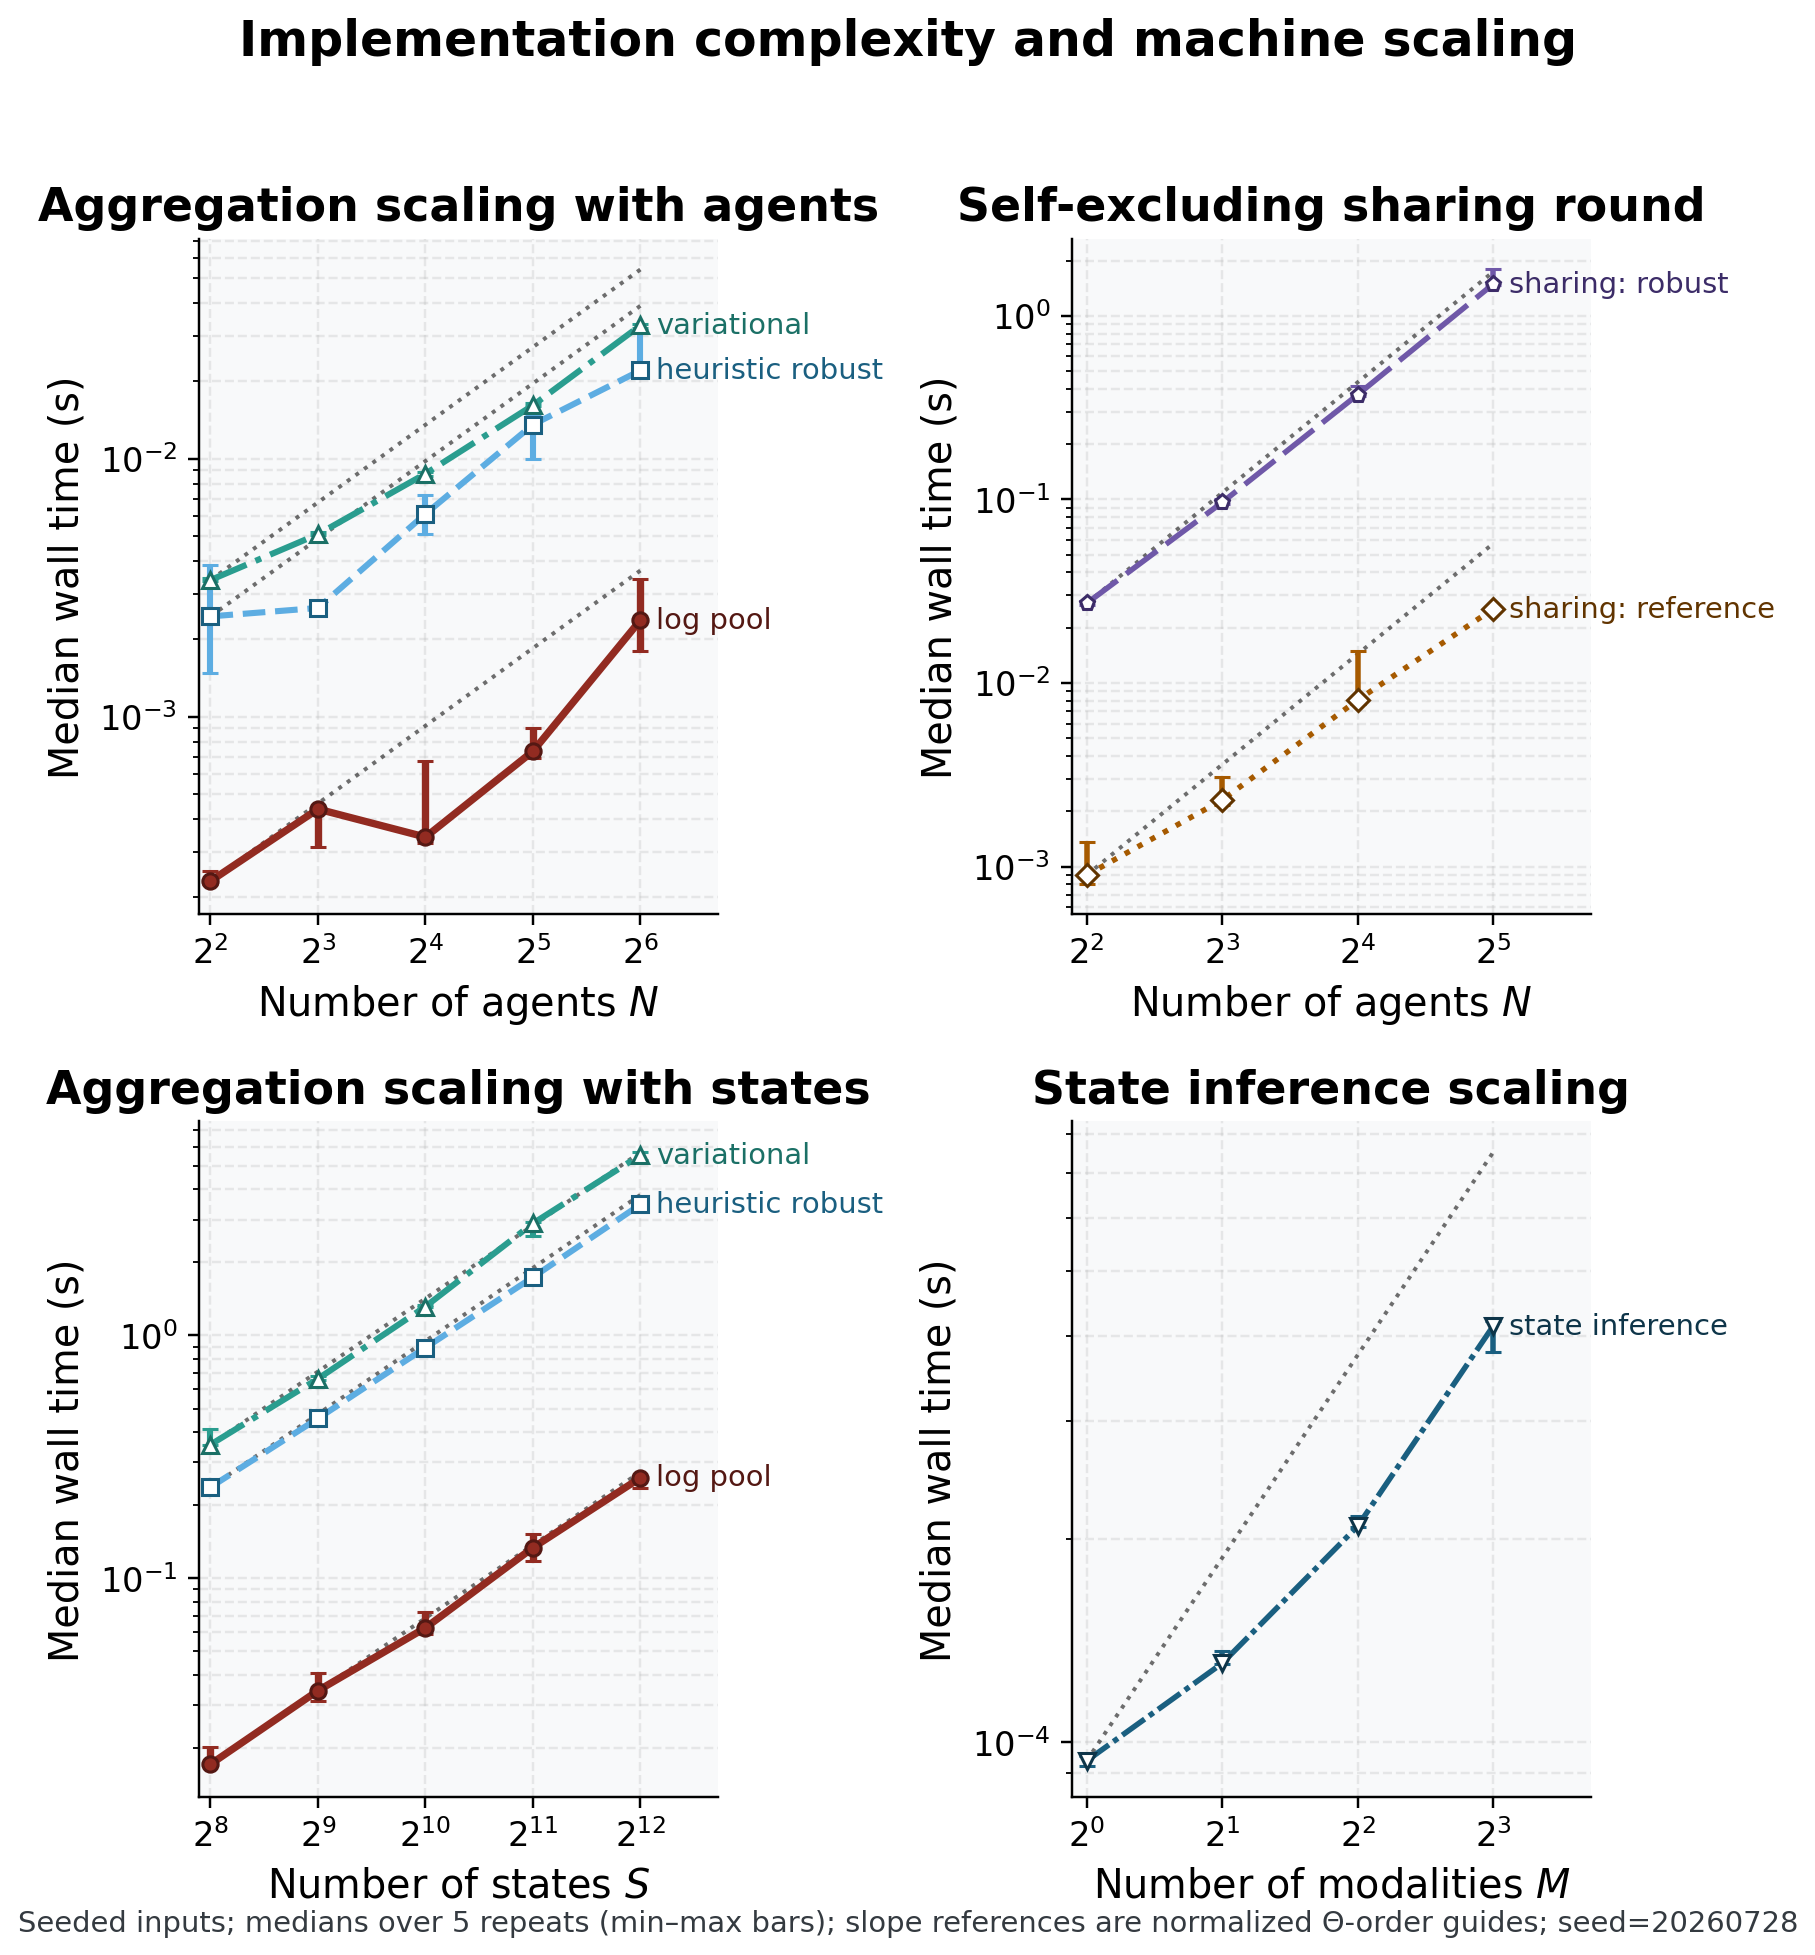
\includegraphics[width=0.95\linewidth,height=0.5\textheight,keepaspectratio,alt={Four-panel log-log timing figure showing median wall-clock scaling with agents, states, and modalities for aggregation, self-excluding sharing, and state inference. Distinct markers, dashes, open fills, and endpoint labels identify operations; error bars show timing spans and dotted lines are normalized order guides.}]{../figures/complexity_scaling.png}
\caption{Implementation-derived complexity and seeded machine-scaling
diagnostic. Source relation: original project computational-complexity
study; estimand: median wall-clock time for categorical aggregation,
naive and iterative self-excluding sharing, and state inference as one
declared dimension changes. The x-axis is agent, state, or modality
count on a log scale; the y-axis is median elapsed seconds on a log
scale. Panels show agent scaling for aggregation, \(N^2\) leave-one-out
sharing, state scaling for aggregation, and modality scaling for
one-step inference. Circle, square, triangle, and additional distinct
marker-and-dash combinations identify simultaneously plotted operations;
open versus filled marks and direct endpoint labels duplicate color.
Vertical whiskers are recorded minimum-to-maximum timing spans around
the median, not confidence intervals. Dark dotted lines are normalized
\(\Theta\)-order guides derived from implementation accounting, not
fitted results. The fixed seeded benchmark ran on \(arm64\) with Python
\(3.12.12\), NumPy \(2.4.2\), seed \(20260728\), and \(5\) measured
repeat(s) after \(1\) warmup(s); timing repeats within each grid point
are the replication unit. These timings support only the implemented
paths, fixed machine, and measured grid; they do not establish an
asymptotic lower bound, portable throughput, distributed scaling, or a
universal hardware benchmark.}\label{fig:complexity-scaling}
\end{figure}

\section{Formalism: recovery limits, EFE, and tempered
aggregation}\label{sec:formalism}

\ifcsname proposition\endcsname
\else
\newtheorem{proposition}{Proposition}
\fi

The primitives of sec.~\ref{sec:methods} are governed by a compact set
of machine-checkable identities.

Their counter is monotone across the methods and this section.
Definitions \ref{def:generalized-bayes} and \ref{def:cavity} cover the
posterior and cavity / PVI update (sec.~\ref{sec:method-genbayes}).
Lemma \ref{lem:renyi-kl-limit} gives the Rényi KL limit
(sec.~\ref{sec:method-divergences}).

Proposition \ref{prop:robust-loss-recovery} gives the \(\beta\)-loss and
rcce NLL limits (sec.~\ref{sec:method-losses}). Theorem
\ref{thm:belief-sharing-recovery} and Corollary
\ref{cor:closed-form-bayes} give belief-sharing and Bayes recovery
(sec.~\ref{sec:method-aggregation}). Proposition
\ref{prop:efe-decomposition} below gives the expected-free-energy
identity.

Each carries a tested residual. None grants a bounded-influence
guarantee to the server-side \breaktt{robust\_aggregate} heuristic; that
boundary is stated in sec.~\ref{sec:robustness-axes}.

\subsection{Recovery limits as the proof
surface}\label{sec:formalism-recovery}

The recovery limits separate client and server claims. The divergence
and loss limits recover the standard-Bayes client update; the
independently tested identity equates \breaktt{robust\_aggregate} with
\texttt{log\_linear\_pool} when \texttt{robustness=0}, recovering the
project's standard server pool. Under the explicit shared-support,
posterior-log-potential, and fixed-weight assumptions in
sec.~\ref{sec:method-aggregation}, that pool is a categorical
specialization of Eq. 7's message-combination term, not recovery of the
complete source protocol \citep{friston2024federated}.

We collect the five residuals that pin those limited claims, each
emitted by the test-suite and reported in
sec.~\ref{sec:results-recovery}, never hardcoded.

Read each row of the table below as a triple: the robust primitive, the
trusting knob value at which it must collapse onto its standard-Bayes or
project-local counterpart, and the tested residual measuring whatever
gap survives at that value. The rows differ in what kind of check they
are.

The divergence and loss rows evaluate inside the implementation's
closed-form switch band, so their zeros are exact branch identities ---
guaranteed by construction, not measurements that could have come out
otherwise.

Their genuine falsifiers are the \emph{off-switch} convergence
residuals, evaluated just outside the band (at \(\alpha = 1.00001\),
\(\beta = 1.00 \times 10^{-6}\),
\(q_{\text{loss}} = 1.00 \times 10^{-6}\)) where the general formulas
run and a nonzero gap is possible: those residuals are
\(1.66 \times 10^{-5}\), \(1.24 \times 10^{-5}\), and
\(1.12 \times 10^{-5}\) respectively, and any failure of those
quantities to shrink toward the limit would falsify the containment
claim.

The posterior row is a measured identity on the general code path, so
its near-zero residual is itself the falsification surface. The
aggregate row's zero at exactly \(c=0\) is likewise branch-exact; the
identity is additionally exercised on the iterative code path at
near-zero robustness, where the consensus must still land on the
log-linear pool to tight tolerance.

\begin{longtable}[]{@{}
  >{\raggedright\arraybackslash}p{(\linewidth - 4\tabcolsep) * \real{0.3333}}
  >{\raggedright\arraybackslash}p{(\linewidth - 4\tabcolsep) * \real{0.3333}}
  >{\raggedright\arraybackslash}p{(\linewidth - 4\tabcolsep) * \real{0.3333}}@{}}
\caption{Recovery residuals: the largest observed discrepancy between
each robust primitive and its standard-Bayes limit, over the recovery
band. Each is a maximum absolute difference in the natural units of the
quantity (pmf entries for the posterior and aggregate rows, nats for the
divergence and loss rows); the aggregate, divergence, and loss rows are
exactly zero (bit-identical) and the posterior row is exact to machine
precision (about one ULP), so the limits are verified identities, not
approximations. The labeled presentation of these residuals lives in
sec.~\ref{sec:results-recovery}.}\tabularnewline
\toprule\noalign{}
\begin{minipage}[b]{\linewidth}\raggedright
Identity (owner statement)
\end{minipage} & \begin{minipage}[b]{\linewidth}\raggedright
Trusting limit
\end{minipage} & \begin{minipage}[b]{\linewidth}\raggedright
Tested residual
\end{minipage} \\
\midrule\noalign{}
\endfirsthead
\toprule\noalign{}
\begin{minipage}[b]{\linewidth}\raggedright
Identity (owner statement)
\end{minipage} & \begin{minipage}[b]{\linewidth}\raggedright
Trusting limit
\end{minipage} & \begin{minipage}[b]{\linewidth}\raggedright
Tested residual
\end{minipage} \\
\midrule\noalign{}
\endhead
\bottomrule\noalign{}
\endlastfoot
Rényi \(\to\) KL (Lemma \ref{lem:renyi-kl-limit},
eq.~\ref{eq:renyi-limit}) & \(\alpha \to 1\) & 0 \\
rcce \(\to\) NLL (Proposition \ref{prop:robust-loss-recovery},
eq.~\ref{eq:rcce-loss}) & \(q_{\text{loss}} \to 0\) & 0 \\
\(\beta\)-loss \(\to\) NLL (Proposition \ref{prop:robust-loss-recovery},
eq.~\ref{eq:beta-loss}) & \(\beta \to 0\) & 0 \\
generalized posterior \(\to\) Bayes (Corollary
\ref{cor:closed-form-bayes}, eq.~\ref{eq:standard-bayes}) & KL, NLL &
5.55e-17 \\
\breaktt{robust\_aggregate} \(\to\) log-linear pool (Theorem
\ref{thm:belief-sharing-recovery}, eq.~\ref{eq:robust-identity}) &
\(c = 0\) & 0 \\
\end{longtable}

The central project identity is the aggregation collapse of
eq.~\ref{eq:robust-identity}: \breaktt{robust\_aggregate(robustness=0)}
equals the log-linear pool eq.~\ref{eq:log-linear-pool}. Its source
bridge is deliberately narrow.

Take the admitted posteriors defined in
sec.~\ref{sec:method-aggregation}, on a finite common support with
\(q_n(s)>0\), and represent each Eq. 7 softmax input as a posterior log
potential \(m_n(s)=\log q_n(s)+\kappa_n\), with \(\kappa_n\) constant in
\(s\) and fixed declared weights \(w_n\) independent of the emerging
consensus. Softmax then cancels the additive constants and yields the
project pool.

This identifies only the source equation's message-combination term; it
does not identify source message construction, cavity/exclusion policy,
scheduling, generative factors, or the complete protocol. Theorem
\ref{thm:belief-sharing-recovery} (sec.~\ref{sec:method-aggregation})
states that specialization and the local \(c=0\) identity; the residual
0 above pins the latter.

Corollary \ref{cor:closed-form-bayes} establishes the separate client
result: \breaktt{generalized\_posterior(KLD,\ NLL)} reproduces the
closed-form prior-times-likelihood Bayes posterior of
eq.~\ref{eq:standard-bayes} to residual 5.55e-17. Pooling such local
posteriors has the stated categorical specialization only under the
theorem's assumptions.

The honesty contract binds here: the theorem and corollary cover only
the recovery identity and the per-agent rigorous axis (Proposition
\ref{prop:robust-loss-recovery}); no statement transfers the
bounded-influence guarantee to the server-side divergence-reweighting
heuristic, whose positive property is the \(\texttt{robustness}=0\)
limit of eq.~\ref{eq:robust-identity}. A scoped no-go rejects a declared
separable objective class without certifying another.

\subsection{Expected-free-energy identity as an algebraic
check}\label{sec:formalism-efe}

The active-inference substrate that drives the studies of
sec.~\ref{sec:results} is a categorical specialization of the
expected-free-energy algebra discussed by Friston et al.
\citep{friston2024federated}. It decomposes the expected free energy of
a policy \(\boldsymbol{\pi}\) into two equivalent two-term forms. The
risk-plus-ambiguity (cost) view and the negated pragmatic-plus-epistemic
(value) view are the same scalar \(G(\boldsymbol{\pi})\) rearranged
\citep{dacosta2020active, friston2024federated}:

\begin{equation}\protect\phantomsection\label{eq:efe-decomposition}{
\begin{aligned}
G(\boldsymbol{\pi})
&= \underbrace{\text{risk} + \text{ambiguity}}_{\text{cost view}}\\
&= -\underbrace{\big(\text{pragmatic} + \text{epistemic}\big)}_{\text{value view}}.
\end{aligned}
}\end{equation}

The two views are not approximations of one another; they are the same
scalar rearranged. In the implementation the shared entropy term enters
both sides of the rearrangement, so the identity residual is zero by
construction --- it is a definitional consistency check on the
decomposition's bookkeeping, not an independent measurement.

The scientific content lives in the per-term semantics, which are pinned
independently of the identity (see the closing clause of the proposition
below):

\begin{equation}\protect\phantomsection\label{eq:efe-identity}{
\begin{aligned}
&\big(\text{risk} + \text{ambiguity}\big)\\
&\quad + \big(\text{pragmatic} + \text{epistemic}\big)
\equiv 0.
\end{aligned}
}\end{equation}

\begin{proposition}[Expected-free-energy decomposition identity]\label{prop:efe-decomposition}
For the categorical model in \breaktt{expected\_free\_energy.py}, the cost and
negated-value forms of (\ref{eq:efe-decomposition}) give the same
$G(\boldsymbol{pi})$; hence (\ref{eq:efe-identity}) holds to machine precision.
Cross-entropy and entropy splits establish the equality.
\end{proposition}

The residual is pinned to \(10^{-9}\). Independent checks require
deterministic likelihoods to give zero ambiguity, uninformative
likelihoods zero epistemic value, and preference-matched predictions
lower risk.

Here risk is \(\mathrm{KL}(q(o\mid\boldsymbol{\pi})\,\|\,p_C(o))\), and
ambiguity is expected likelihood entropy
\(\mathbb{E}_{q(s)}[H[p(o\mid s)]]\).

Pragmatic value is expected log-preference
\(\mathbb{E}_{q_{\boldsymbol{\pi}}(o)}[\ln p_C(o)]\). Epistemic value is
the state-outcome mutual information
\(H[q_{\boldsymbol{\pi}}(o)] - \mathbb{E}_{q(s)}[H[p(o\mid s)]]\).

The executed formal-specialization diagnostic of
fig.~\ref{fig:efe-decomp} uses a uniform prior over the nine locations.
This is intentional: the canonical sentinel-world \(D_0\) is a point
mass at the den, and under that fully resolved prior the
mutual-information term is zero because there is no state uncertainty
for an observation to reduce.

The uncertainty-bearing diagnostic makes the epistemic term visible
without changing the canonical \(D_0\) used by the inference and
recovery studies. Thus a near-zero epistemic value is a meaningful null
condition, not a missing term.

fig.~\ref{fig:efe-decomp} shows the additive risk-plus-ambiguity view
beside a signed pragmatic/epistemic waterfall whose terminal endpoint is
\(G(\boldsymbol{\pi})\), labels epistemic value as
\(I(s;o\mid\boldsymbol{\pi})\), and annotates the identity residual; it
visualizes Proposition \ref{prop:efe-decomposition}, not a fitted
result, so it carries no error bars.

\begin{figure}
\centering
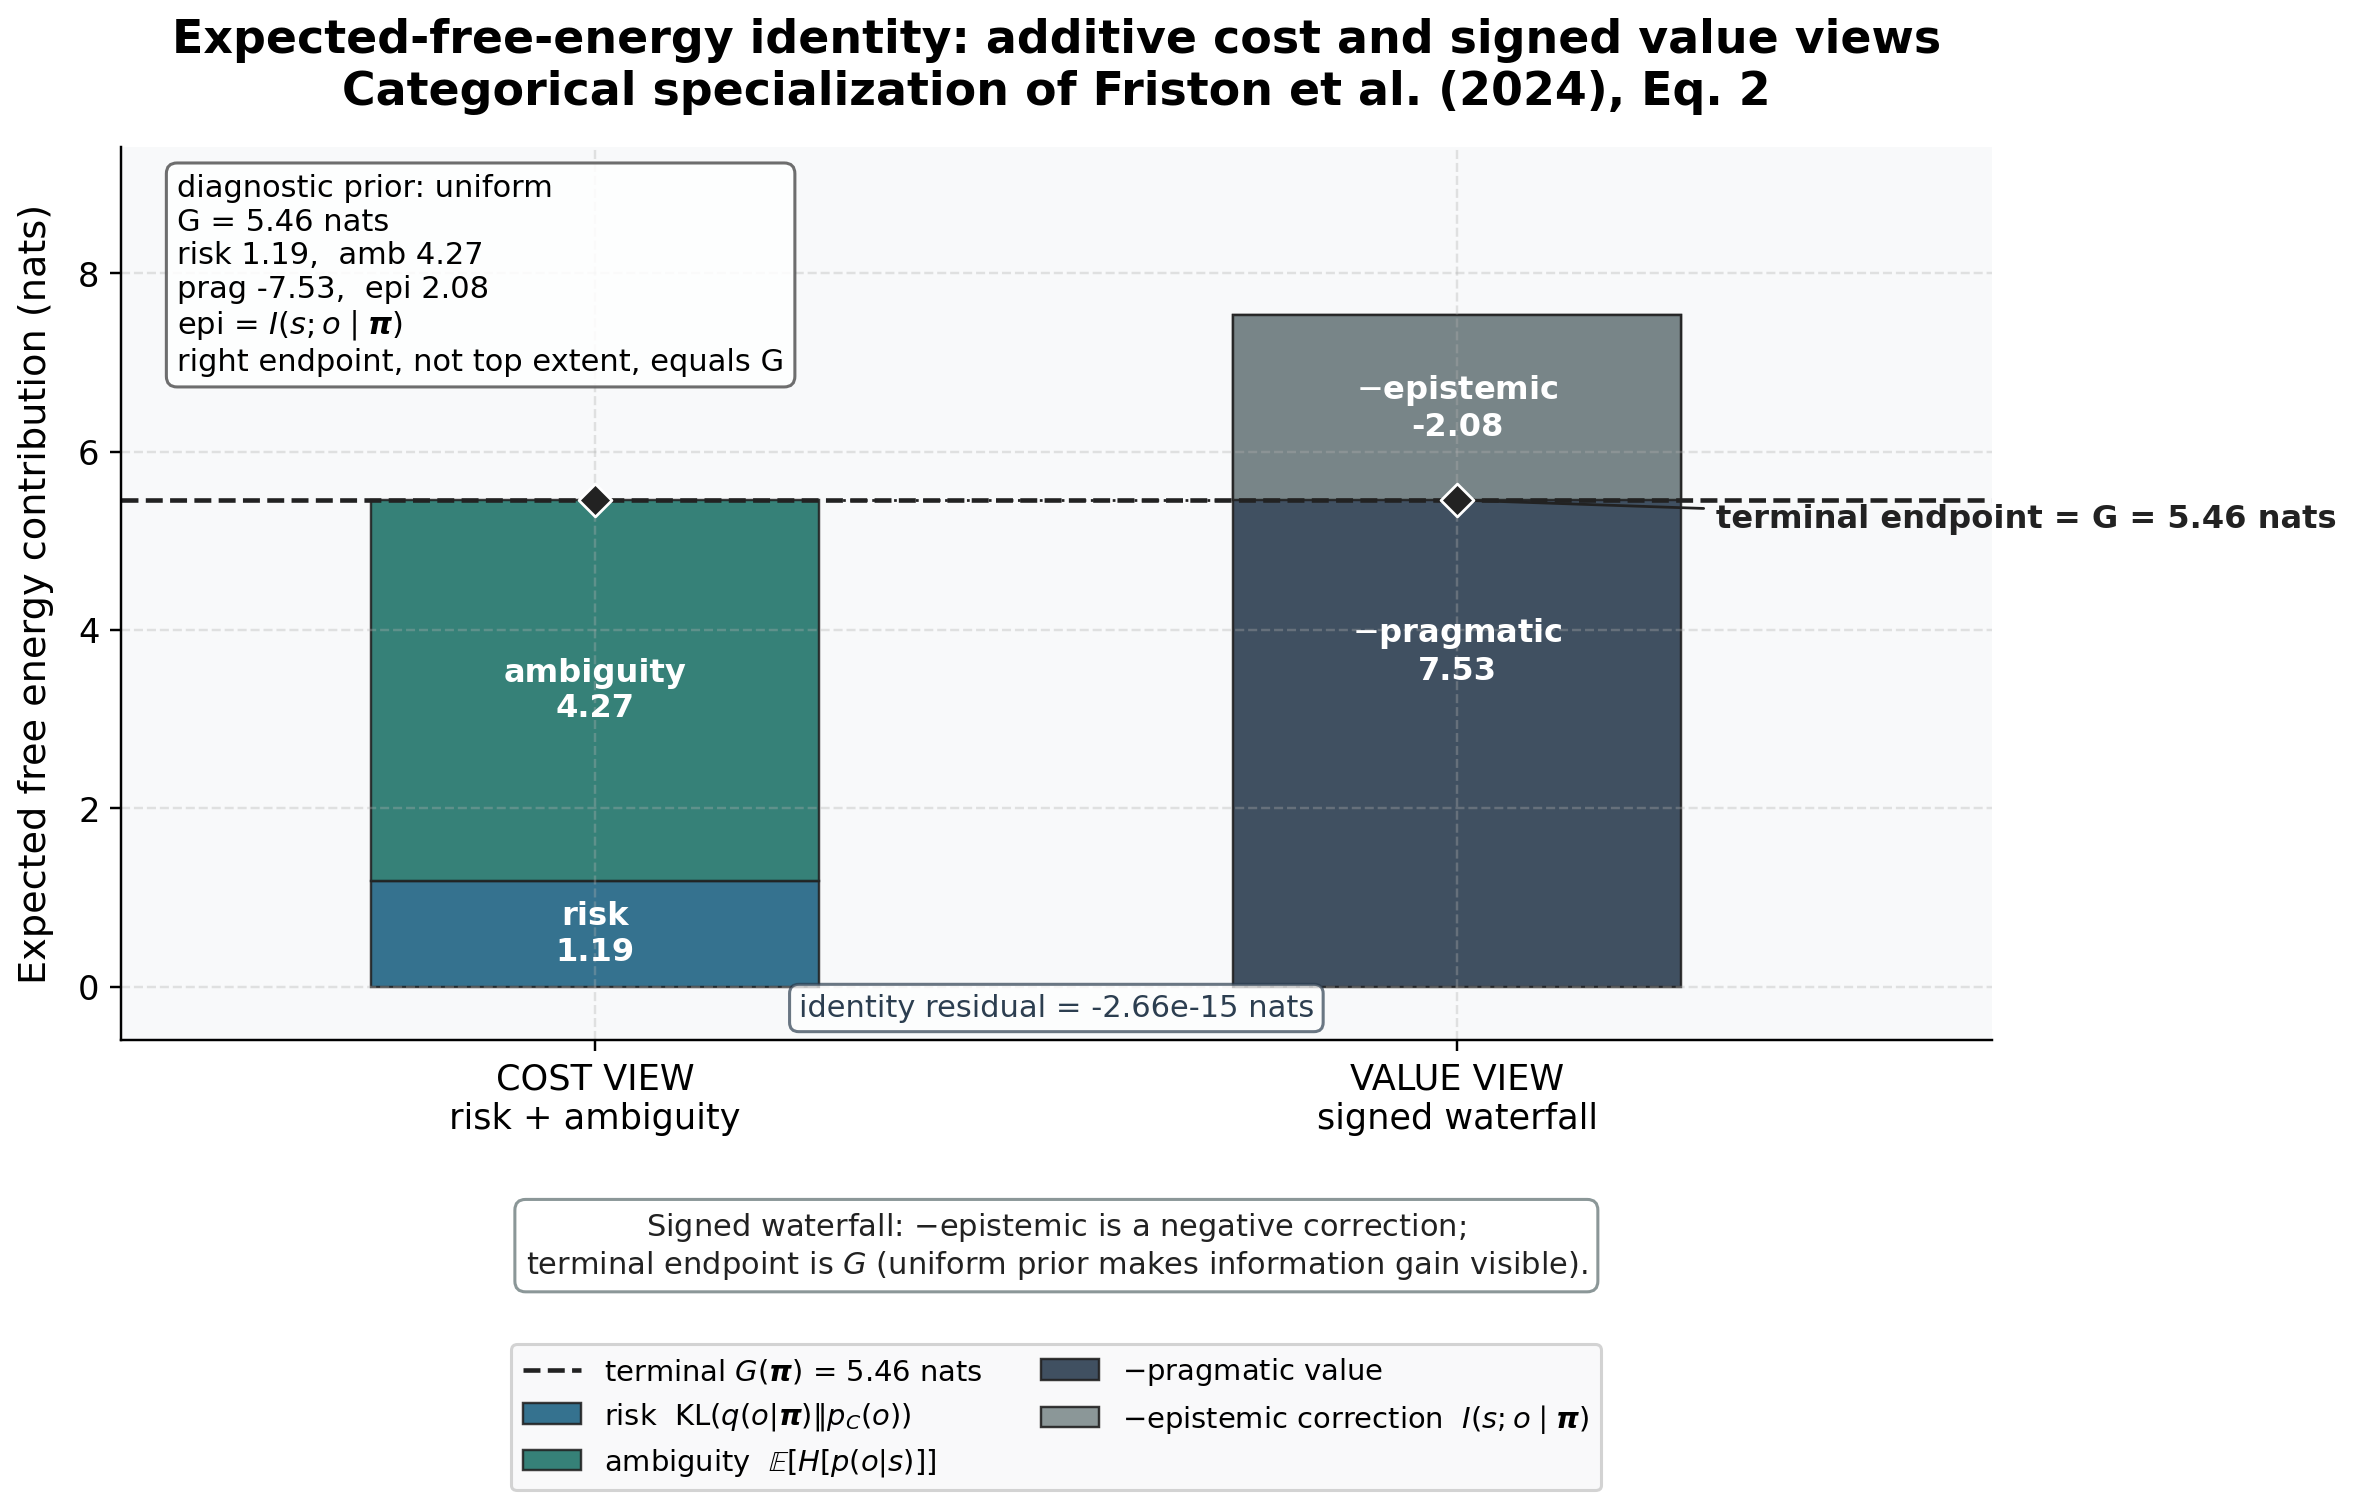
\includegraphics[width=0.85\linewidth,height=0.5\textheight,keepaspectratio,alt={Two views of a categorical expected-free-energy identity in nats. The left stack shows risk plus ambiguity; the right signed waterfall shows pragmatic value and a negative epistemic correction ending at the same terminal value.}]{../figures/efe_decomposition.png}
\caption{Expected-free-energy decomposition for the categorical
generative model (expected\_free\_energy.py). Source relation: formal
specialization of Friston et al.~(2024), Eq. 2; estimand: categorical
EFE identity in nats. x-axis: two views of the same identity (left,
additive cost view: risk + ambiguity; right, signed value waterfall:
positive minus-pragmatic contribution followed by a negative epistemic
correction). y-axis: EFE contribution in nats. The heavy endpoint marker
and connector, rather than the intermediate top extent, identify the
terminal \(G(\boldsymbol{\pi})\) value. The epistemic term is
state--outcome mutual information \(I(s;o\mid\boldsymbol{\pi})\); it is
visible because the diagnostic prior is uniform, whereas the canonical
point-mass \(D_0\) is the corresponding zero-information null. The
finite terms satisfy the identity at machine precision. This
deterministic algebraic check has no error bars or independent sample
size, and it does not reproduce every parameter-learning term in the
source equation.}\label{fig:efe-decomp}
\end{figure}

The expected-free-energy identity of eq.~\ref{eq:efe-identity} is the
action-selection counterpart of the inference-side recovery limits
collected above: both are exact, closed-form, machine-checkable
identities over the same categorical generative model.

Together they establish that the FedGVI-federated active-inference
colony of this work is built on verified algebra throughout --- the
per-agent generalized-Bayes update recovers standard Bayes, the
aggregation recovers the project log-linear pool under its qualified
categorical bridge, and the policy scoring decomposes exactly --- so
every robustness result in sec.~\ref{sec:results} is a controlled
departure from a known, tested fixed point rather than an unmoored
claim.

\subsection{Tempered aggregation free energy and the accuracy-guarantee
trade}\label{sec:formalism-tempered}

The recovery limits and the expected-free-energy identity fix the
\emph{endpoints} of the aggregation family; the remaining formal
question is what a controlled departure from the unit-entropy server
buys and what it costs. The objective-backed variational aggregator of
sec.~\ref{sec:supp-variational} holds its consensus-entropy term at unit
weight.

Freeing that single coefficient produces a one-parameter family whose
only moving part is the sharpness of the consensus, and whose raw
effective-weight bound is provably untouched. The following proposition
isolates exactly that separation --- algebra that moves versus algebra
that does not --- before the interpretation subsections turn to the
empirical accuracy question the algebra cannot settle on its own.

\begin{proposition}[Tempered aggregation free energy]\label{prop:tempered-aggregation}
Let $lambda > 0$ and let $F_lambda$ be (\ref{eq:tempered-family}). At fixed $a$,
the $q$-minimizer is (\ref{eq:tempered-updates}). At
$lambda = 1.0$, $F_lambda$ and both updates equal
the standard variational aggregate bit-for-bit. The $a$-update and bound
$a_n \le w_n$ omit $lambda$ and hold for every $lambda > 0$.
\end{proposition}

At that default, the endpoint-selection rule also reduces bit-for-bit to
the standard variational aggregate (Definition
\ref{def:aggregation-free-energy}; sec.~\ref{sec:supp-variational}).

The proposition is intentionally more specific than the phrase
``temperature improves robustness.'' It identifies exactly which part of
the variational server changes when the entropy coefficient changes, and
it separates that algebra from the empirical accuracy question.

The objective and its update rules are a generalized-Bayes construction
in the sense of \citep{bissiri2016general, knoblauch2022generalized},
while the particular client/server decomposition is the one implemented
and tested here.

\subsubsection{What the entropy weight
controls}\label{sec:formalism-tempered-interpretation}

For a fixed effective-weight vector \(a\) and \(\lambda>0\), the
\(q\)-block in eq.~\ref{eq:tempered-updates} is a weighted geometric
pool of the local posteriors with inverse temperature \(1/\lambda\).
Lower \(\lambda\) concentrates more sharply on states that receive
consistent log-belief support; larger \(\lambda\) spreads probability
mass and retains more entropy.

As \(\lambda\downarrow0\), the positive-temperature expression
approaches a winner-take-most consensus (subject to ties and finite
numerical support), whereas large \(\lambda\) approaches a flatter
distribution. The implementation exposes that endpoint as a separately
defined deterministic tied-argmax rule; it does not substitute
\(\lambda=0\) into the objective or coordinate update.

This is a controlled change in the consensus geometry, not an automatic
outlier detector.

The coupling matters. Although the formula for the \(a\)-block does not
contain \(\lambda\), the fixed point can still change because \(a_n\) is
evaluated at the new \(q\).

The correct statement is therefore conditional: for any current
consensus, the effective-weight update and the raw bound \(a_n\leq w_n\)
are unchanged; after alternating updates, different temperatures can
reach different coupled \((q,a)\) fixed points. This distinction
prevents the temperature result from being read as a theorem that the
normalized influence or accuracy is invariant in \(\lambda\).

\subsubsection{Recovery at the qualified log-linear-pool
corner}\label{sec:formalism-tempered-recovery}

At the configured default \(\lambda=1.0\), the entropy coefficient is
the unit coefficient used by the original variational aggregator. The
implementation therefore recovers that aggregator bit-for-bit, including
its block updates and its endpoint-selection rule.

Turning the robustness strength \(c\) to zero then sets every server
weight to its base value and gives the tempered log-linear pool. At the
default temperature this is the ordinary log-linear pool of
eq.~\ref{eq:log-linear-pool}.

Under the shared-support, posterior-log-potential, and fixed-weight
assumptions of sec.~\ref{sec:method-aggregation}, that is the
categorical specialization of Eq. 7's message-combination term; it is
not the complete belief-sharing protocol of
\citep{friston2024federated}. Away from that default, the result is a
tempered generalization of the pool and should not be described as
Friston's Eq. 7 itself.

This nested limit is useful for interpretation. The \(c\to0\) limit
identifies the aggregation family with a known consensus operator; the
\(\lambda=1.0\) slice identifies the objective-backed implementation
used in the main server comparison.

Neither limit grants the server-side \breaktt{robust\_aggregate}
heuristic a variational objective or a bounded-influence guarantee. The
FedGVI literature's rate and robustness results remain attached to their
stated loss, divergence, and sampling assumptions
\citep{mildner2025fedgvi, mildner2025rates}.

\subsubsection{What the accuracy--guarantee trade can
establish}\label{sec:formalism-tempered-evidence}

The executed grid over \(\lambda\in\{0.1, 0.2, 0.3, 0.5, 0.7, 1\}\) is a
finite sensitivity study, not a search over a continuous optimum. It
asks whether any tested temperature narrows the point-accuracy gap to
the sharp heuristic while retaining the same effective-weight update.
The closest tested temperature is \(\lambda^{\ast}=0.3\), with observed
gap \(0.0008\).

These tokens are computed from the executed contaminated-colony trials
and are reported with the grid definition so a reader can reproduce the
selection rule.

The result has two distinct readings. If a lower temperature improves
the paired point-accuracy comparison, it provides design evidence that
entropy regularization can be tuned rather than accepted as a fixed
conservatism penalty.

If no tested temperature closes the gap, that negative result is still
informative: within this objective family, the same entropy mechanism
that keeps consensus diffuse can limit exact point recovery under
confident contamination.

In either case, the grid does not identify a universally best
temperature, establish minimax robustness, or transfer the variational
raw weight bound to a different estimator. Generalized-Bayes calibration
and robust-loss theory motivate the family, but only the executed
categorical design supports the present finite-grid statement
\citep{bissiri2016general, knoblauch2022generalized, mildner2025fedgvi}.

\subsubsection{Publication-facing
interpretation}\label{sec:formalism-tempered-interpretation-summary}

The practical contract is consequently three-part. Use the default
temperature when exact compatibility with the tested variational server
is the priority.

Explore the declared grid when the application can trade concentration
against the same raw effective-weight control.

Treat any selected temperature as a configuration-specific empirical
choice until it is tested under a new contamination mechanism, colony
size, sensor model, or loss. This is the appropriate bridge between the
formal objective and the active-inference setting: it exposes a tunable
consensus geometry while keeping recovery, guarantee, and accuracy
claims on separate evidence tracks.

\section{Results: recovery checks and study suite}\label{sec:results}

Every quantitative assertion in this and the following results sections
is a generated token, hydrated by the manuscript-variable generator from
analysis outputs produced by \breaktt{src/analysis/workflow.py} and
\breaktt{src/fedference/experiments/} --- no number is transcribed by
hand.

The studies implement categorical source-mechanism analogues of the
colony belief-sharing scenario \citep{friston2024federated} and add the
contaminated-sentinel robustness sweep and the federated neural-network
baseline that are this paper's robust-federated-learning contribution.
All runs are deterministic under seed 0.

We lead with the recovery limits, not with a study, because they are
what makes the studies a single coherent system rather than a collection
of unrelated experiments. The generalized-Bayes machinery of
sec.~\ref{sec:methods} contains the standard-Bayes client corner, while
the server has the exact project-local zero-robustness log-linear-pool
identity.

Under the explicit bridge in sec.~\ref{sec:method-aggregation}, that
pool is a categorical specialization of Eq. 7's message-combination term
rather than the complete source protocol. We verify those limited
identities to machine precision before reporting anything built on top
of them.

\subsection{Recovery limits: standard-Bayes and project-pool corners are
exact to machine precision}\label{sec:results-recovery}

The identities that anchor every result are the client recovery of
standard Bayes at the KL/NLL/\(\beta\to0\) and \(q_{\text{loss}}\to0\)
limits plus the project-local server recovery to the log-linear pool at
\(c=0\) --- the scoped claims of sec.~\ref{sec:formalism} (Corollary
\ref{cor:closed-form-bayes}, Lemma \ref{lem:renyi-kl-limit}, Theorem
\ref{thm:belief-sharing-recovery}).

These are not figures but exact equalities, pinned by the locked core
test suite.

Under the theorem's shared-support, posterior-log-potential, and
fixed-weight assumptions, the server pool specializes Eq. 7's
message-combination term; it does not reproduce the source construction
in full. Robustness is a tested extension that vanishes at the stated
recovery limits.

The five residuals below are the maximum absolute deviations between
each generalized-Bayes object and the standard object it must reproduce
in the trusting limit.

Each is a deterministic constant of the mathematics, not a per-run
sample: it is reported as the maximum absolute deviation over the
recovery band, which is exactly \(0\) where the implementation evaluates
the closed form at the limit (the Rényi/loss switch) and otherwise a
tiny floating-point residual:

\textbf{Server recovery.} The server-side aggregator at zero robustness
equals the log-linear pool (eq.~\ref{eq:robust-identity}, Theorem
\ref{thm:belief-sharing-recovery}): maximum absolute deviation 0. This
is the \emph{naive-recovery} limit of the server-side heuristic --- the
only property proven for that axis (see sec.~\ref{sec:robustness-axes}).

\textbf{Posterior recovery.} The generalized posterior under the KL
divergence and the NLL loss equals the closed-form
prior\(\times\)likelihood Bayes posterior (eq.~\ref{eq:standard-bayes},
Corollary \ref{cor:closed-form-bayes}): maximum absolute deviation
5.55e-17.

\textbf{Divergence recovery.} The Rényi divergence recovers KL as
\(\alpha\to1\) (eq.~\ref{eq:renyi-limit}, Lemma
\ref{lem:renyi-kl-limit}): residual 0.

\textbf{Loss recoveries.} The \(\beta\)-loss recovers the NLL as
\(\beta\to 0\) (eq.~\ref{eq:beta-loss}, Proposition
\ref{prop:robust-loss-recovery}): residual 0. The robust categorical
cross-entropy recovers the NLL as \(q_{\text{loss}}\to 0\)
(eq.~\ref{eq:rcce-loss}, Proposition \ref{prop:robust-loss-recovery}):
residual 0.

Because the Rényi divergence and the two categorical losses switch to
their exact closed form inside narrow numerical-stability bands around
the limit point (the Rényi switch band for \(\alpha\) and the
categorical-loss switch band for \(q_{\text{loss}}\) and \(\beta\)), the
three zero residuals above confirm that branch equals the standard
object --- not, by themselves, that the \emph{general} formula converges
there.

As a genuine (non-branch) convergence witness, evaluating each general
formula strictly \emph{outside} its switch band ---
\(q_{\text{loss}} = \beta =
1.00 \times 10^{-6}\) for the categorical losses and
\(\alpha = 1.00001\) for the Rényi divergence --- gives residuals
1.12e-05 (rcce), 1.24e-05 (\(\beta\)-loss), and 1.66e-05 (Rényi).

These residuals are nonzero---a small multiple of the input offset
itself, as the first-order Taylor behavior near the limit predicts---yet
remain several orders of magnitude below the \(O(1)\) scale of the
loss/divergence values being compared, and shrinking monotonically as
the offset shrinks toward the switch band. The verification is in
\breaktt{test\_core\_identities.py} under \breaktt{tests/fedference/}.

This is evidence that the general formula itself converges to the
standard-Bayes limit, not merely that the implementation switches to it
exactly at the corner.

The first residual is the naive-aggregate limit of the
\emph{server-side} heuristic (Theorem
\ref{thm:belief-sharing-recovery}); the latter four are the per-agent
generalized-Bayes recoveries (Corollary \ref{cor:closed-form-bayes} +
Proposition \ref{prop:robust-loss-recovery}) and the divergence-family
recovery in the Rényi limit (Lemma \ref{lem:renyi-kl-limit},
eq.~\ref{eq:renyi-limit}) that define the theorem-bearing FedGVI axis
under matching assumptions.

Keeping the three axes distinct at the level of the recovery limits is
what lets the robustness claims of sec.~\ref{sec:results-robustness} and
sec.~\ref{sec:results-baseline} rest on the per-agent axis without
leaning on the heuristic.

266 of 268 acceptance criteria are verified. The pure-NumPy/SciPy core
carries project test coverage of 90.57\% (gate \(\ge 90\%\)), with every
stochastic step threaded through a single seeded
\breaktt{np.random.default\_rng(0)}. sec.~\ref{sec:reproducibility}
records the full environment fingerprint, and the expected-free-energy
identity that underwrites the active-inference substrate is proven and
visualized in sec.~\ref{sec:formalism-efe} (fig.~\ref{fig:efe-decomp}).

\subsection{Belief sharing lowers free energy at the project-pool
corner}\label{sec:results-belief_sharing}

With the standard-Bayes client limit and project-pool recovery identity
pinned exactly (sec.~\ref{sec:results-recovery}), the study suite opens
one step away from them. Its estimand is the paired, seed-level
difference in colony-mean variational free energy between incommunicado
and communicating conditions. The design is a categorical
source-mechanism analogue of the colony belief-sharing result
\citep{friston2024federated}.

A colony of 7 sentinels observes one hidden location through independent
noisy sensors of acuity 0.55. Each agent forms a one-step posterior. The
communicating condition applies one standard log-linear-pool round at
the \texttt{robustness=0} recovery corner (eq.~\ref{eq:robust-identity},
eq.~\ref{eq:belief-round}); the incommunicado condition retains the
paired private posteriors.

Under shared support, posterior-log-potential admission, and fixed
weights, the pool specializes Eq. 7's message-combination term. It does
not reproduce the complete source protocol. The paired comparison gives
the following declared quantities:

\textbf{Communicating mean.} \(\bar F_{\text{share}} = 13.2190\)
(across-seed 95\% bootstrap CI \([12.9656, 13.4685]\) over \(n = 480\)
seeds). The single illustrative seed-0 run has its own colony mean
\(15.8115\).

Its per-agent 95\% bootstrap CI is \([15.6177, 16.0647]\) over its
\(n = 7\) agents. That interval characterizes the displayed run's
per-agent spread, not the across-seed mean.

\textbf{Incommunicado mean.} \(\bar F_{\text{solo}} = 16.5298\).

\textbf{Paired reduction from sharing.}
\(\Delta \bar F = \bar F_{\text{solo}} - \bar F_{\text{share}}
= 3.3109\); positive values mean lower free energy under communication.

Each seed supplies one matched pair of colony means. Seeds are the
independent unit; agents are nested within each seed and are not
additional independent replicates. Across the declared seeds, the
communicating condition also has higher mean true-state accuracy
(0.7302) and lower mean surprise (0.3775). These are conditional results
for the reduced protocol.

\begin{figure}
\centering
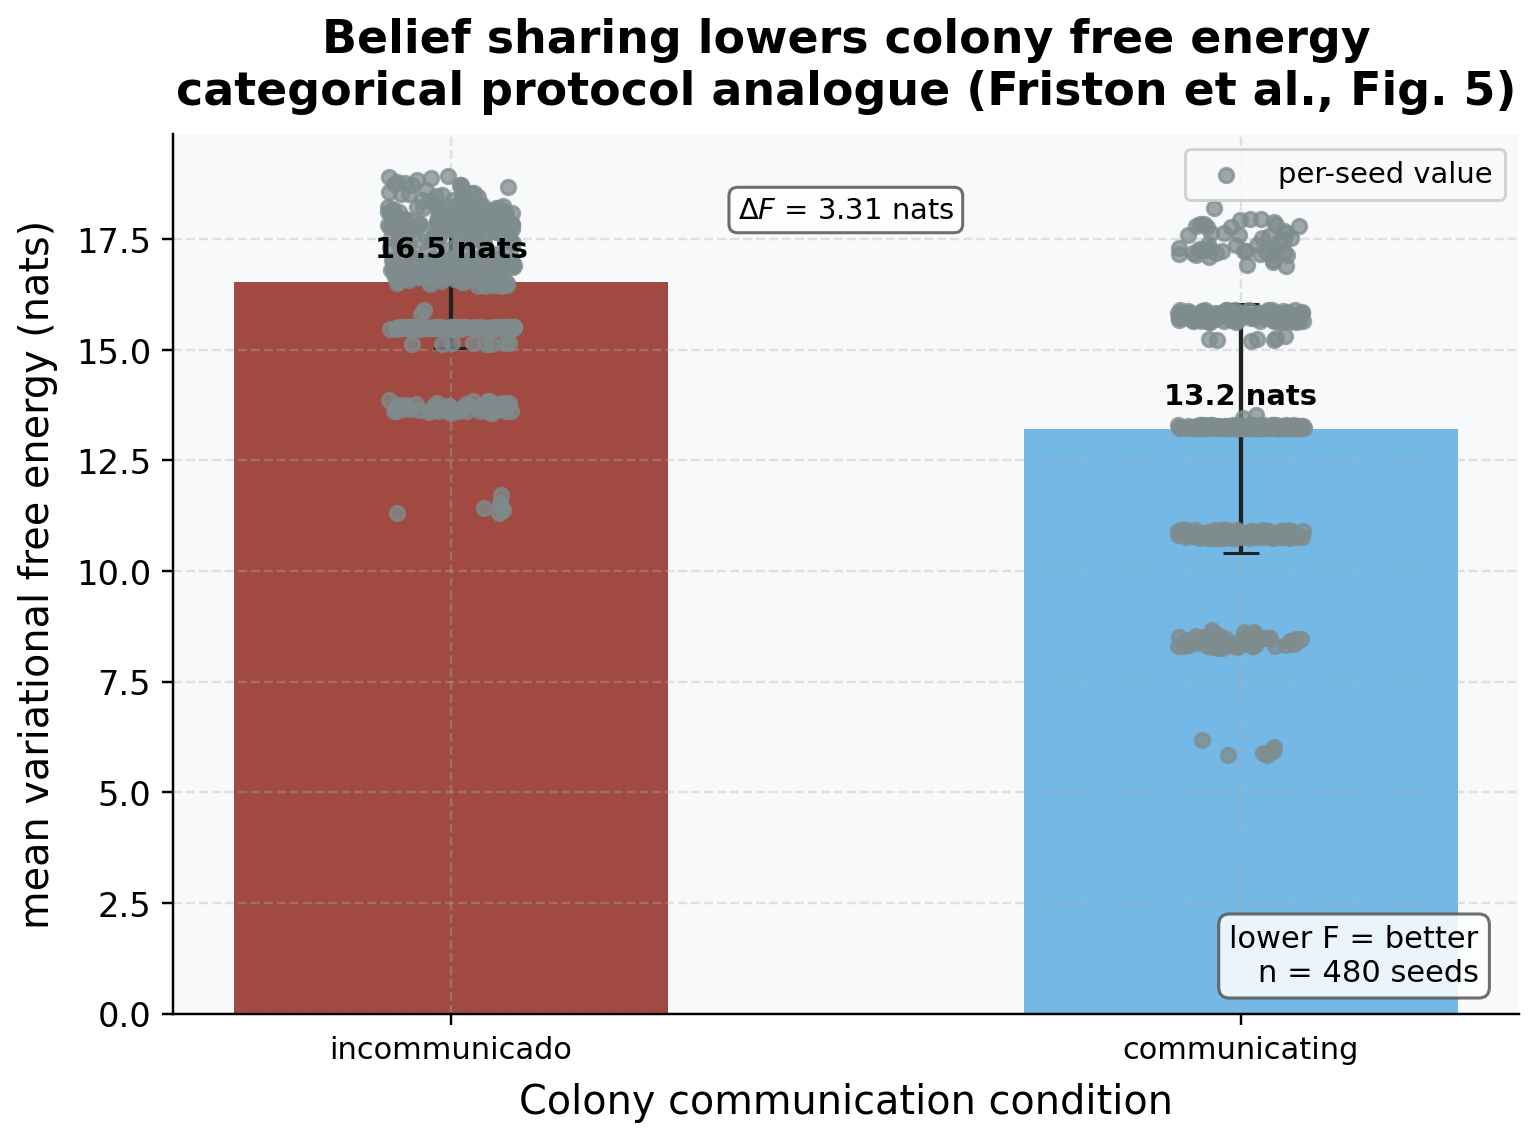
\includegraphics[width=0.8\linewidth,height=0.5\textheight,keepaspectratio,alt={A paired estimation plot joins each seed's filled-circle incommunicado and open-diamond communicating free energy, then shows open-diamond differences, a dotted zero rule, and the percentile-bootstrap interval of incommunicado minus communicating values. Positive differences mean lower free energy with communication.}]{../figures/free_energy_comparison.png}
\caption{Paired colony-mean variational free energy under communication
and isolation. Source relation: reduced categorical source-mechanism
analogue of Friston et al.~(2024), Fig. 5; estimand: seed-level
\(\Delta\bar F=\bar F_{\mathrm{solo}}-\bar F_{\mathrm{share}}\) in nats,
where positive values indicate lower free energy with communication. In
Panel A, the x-axis is communication condition and the y-axis is
colony-mean free energy. Filled reference circles mark incommunicado
values, open comparison diamonds mark communicating values, fine
connecting slopes preserve within-seed pairing, and open diamonds joined
by a dark line identify condition means. In Panel B, the x-axis is
paired difference and the y-axis is jitter only, with one open diamond
per seed, a translucent distribution envelope, a dark dotted zero rule,
and an open-diamond mean with its 95\% percentile-bootstrap interval.
The mean difference is 3.3109 nats across \(n=480\) independent seeds.
Agents and ordered steps remain nested within seed; the interval
resamples seeds, not agents, worlds, or deployments. This
reduced-protocol result does not establish a general communication
benefit or exact source-protocol replication.}\label{fig:free-energy}
\end{figure}

fig.~\ref{fig:free-energy} reports the headline gap;
fig.~\ref{fig:belief-heatmap} shows the per-agent mechanism behind it.

\begin{figure}
\centering
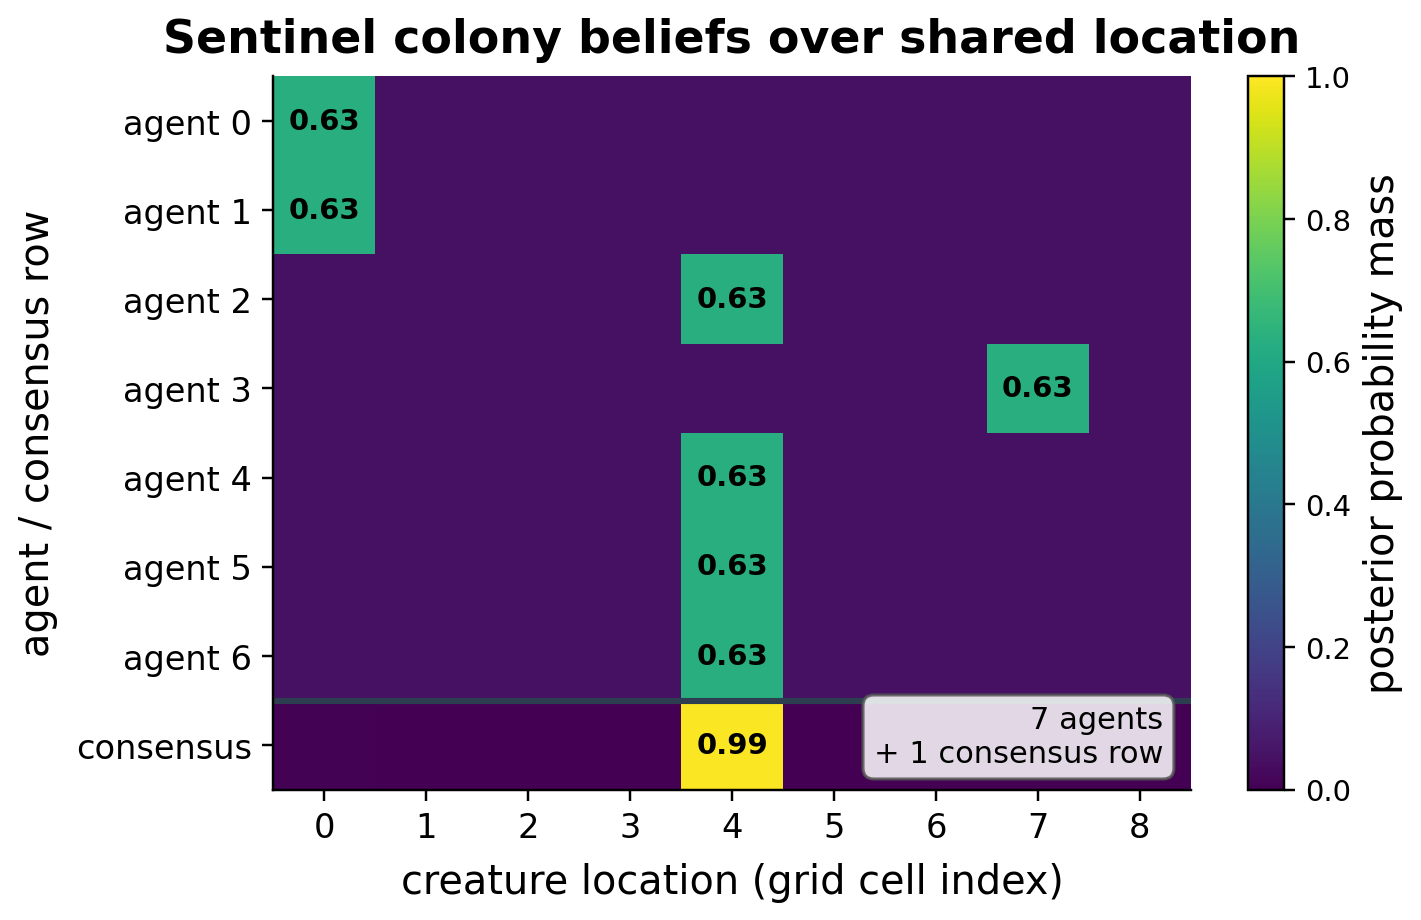
\includegraphics[width=0.8\linewidth,height=0.5\textheight,keepaspectratio,alt={Heatmap of posterior probability over nine location cells for seven agent rows and a consensus row. Agent mass is dispersed, while the consensus row concentrates near one cell.}]{../figures/belief_heatmap.png}
\caption{Single-panel belief heatmap over the hidden creature location.
Source relation: original project diagnostic supporting the Study 1
analogue; estimand: posterior probability mass by hidden state;
uncertainty: deterministic single-seed display. The hidden creature
location (\(7\) sentinels, acuity \(0.55\), seed \(0\)). x-axis:
hidden-state grid cell (creature location, \(9\) cells); rows: the \(7\)
individual agents' private posteriors (one row per agent, dominant cell
annotated), plus a bottom consensus row --- separated by the divider
line --- holding the federated consensus fused from those posteriors by
the cavity-exclusion round defined in the methods. Each private
posterior concentrates only moderately on the cell its noisy observation
suggests; the consensus row concentrates more sharply on the true
location. All cell values are deterministic posterior probabilities for
the single displayed seed, so no error band applies. This mechanism
display does not establish calibration, a general communication benefit,
or exact source-protocol replication.}\label{fig:belief-heatmap}
\end{figure}

\subsubsection{Three robustness axes remain distinct in the
results}\label{sec:robustness-axes-results}

The authoritative three-axis guarantee map is
sec.~\ref{sec:robustness-axes}. The contaminated studies keep its
source-conditional client update, heuristic server reweighting, and
objective-backed variational server rule visually and inferentially
separate. In particular, no result below transfers the client's
bounded-influence theorem or the variational rule's raw-weight bound to
\breaktt{robust\_aggregate}.

\subsection{Conjugate Dirichlet likelihood-learning
trajectory}\label{sec:results-language}

Where the first study fused fixed beliefs in a single round, the second
records the KL trajectory produced when a single agent updates the
likelihood of its shared world. The design is a categorical
source-mechanism analogue of the language-acquisition mechanism
discussed by Friston et al. \citep{friston2024federated}.

Each configured seed runs an agent that learns the likelihood of its
shared world by conjugate Dirichlet updates over 24 count batches, the
count update eq.~\ref{eq:dirichlet-update}. The recorded trajectory is
\(\mathrm{KL}(\text{true } A \,\|\, \text{learned } A)\) before each
batch --- it starts at the flat-prior value and declines monotonically
toward zero as the configured conjugate counts accumulate.

The KL here is the same divergence whose \(\alpha\to1\) Rényi limit is
established by Lemma \ref{lem:renyi-kl-limit}
(eq.~\ref{eq:renyi-limit}), so the learning curve and the recovery
limits measure the same object.

The endpoint summary is: initial KL (flat prior), 3.4231; final KL after
24 batches, 0.0027; and total KL reduction, 3.4204.

The trajectory contains 25 ordered learning steps per seed. Pointwise
95\% intervals resample the \(n = 480\) independent seeds, and the
computed monotone-decreasing indicator is Yes.

The observed decline to a final KL of 0.0027 is the bounded result:
under the tested count schedule, the learned likelihood moves toward the
true generative likelihood as conjugate counts accumulate. This finite
trajectory characterizes the configured update and is not a
convergence-rate result for arbitrary data-generating processes.

\begin{figure}
\centering
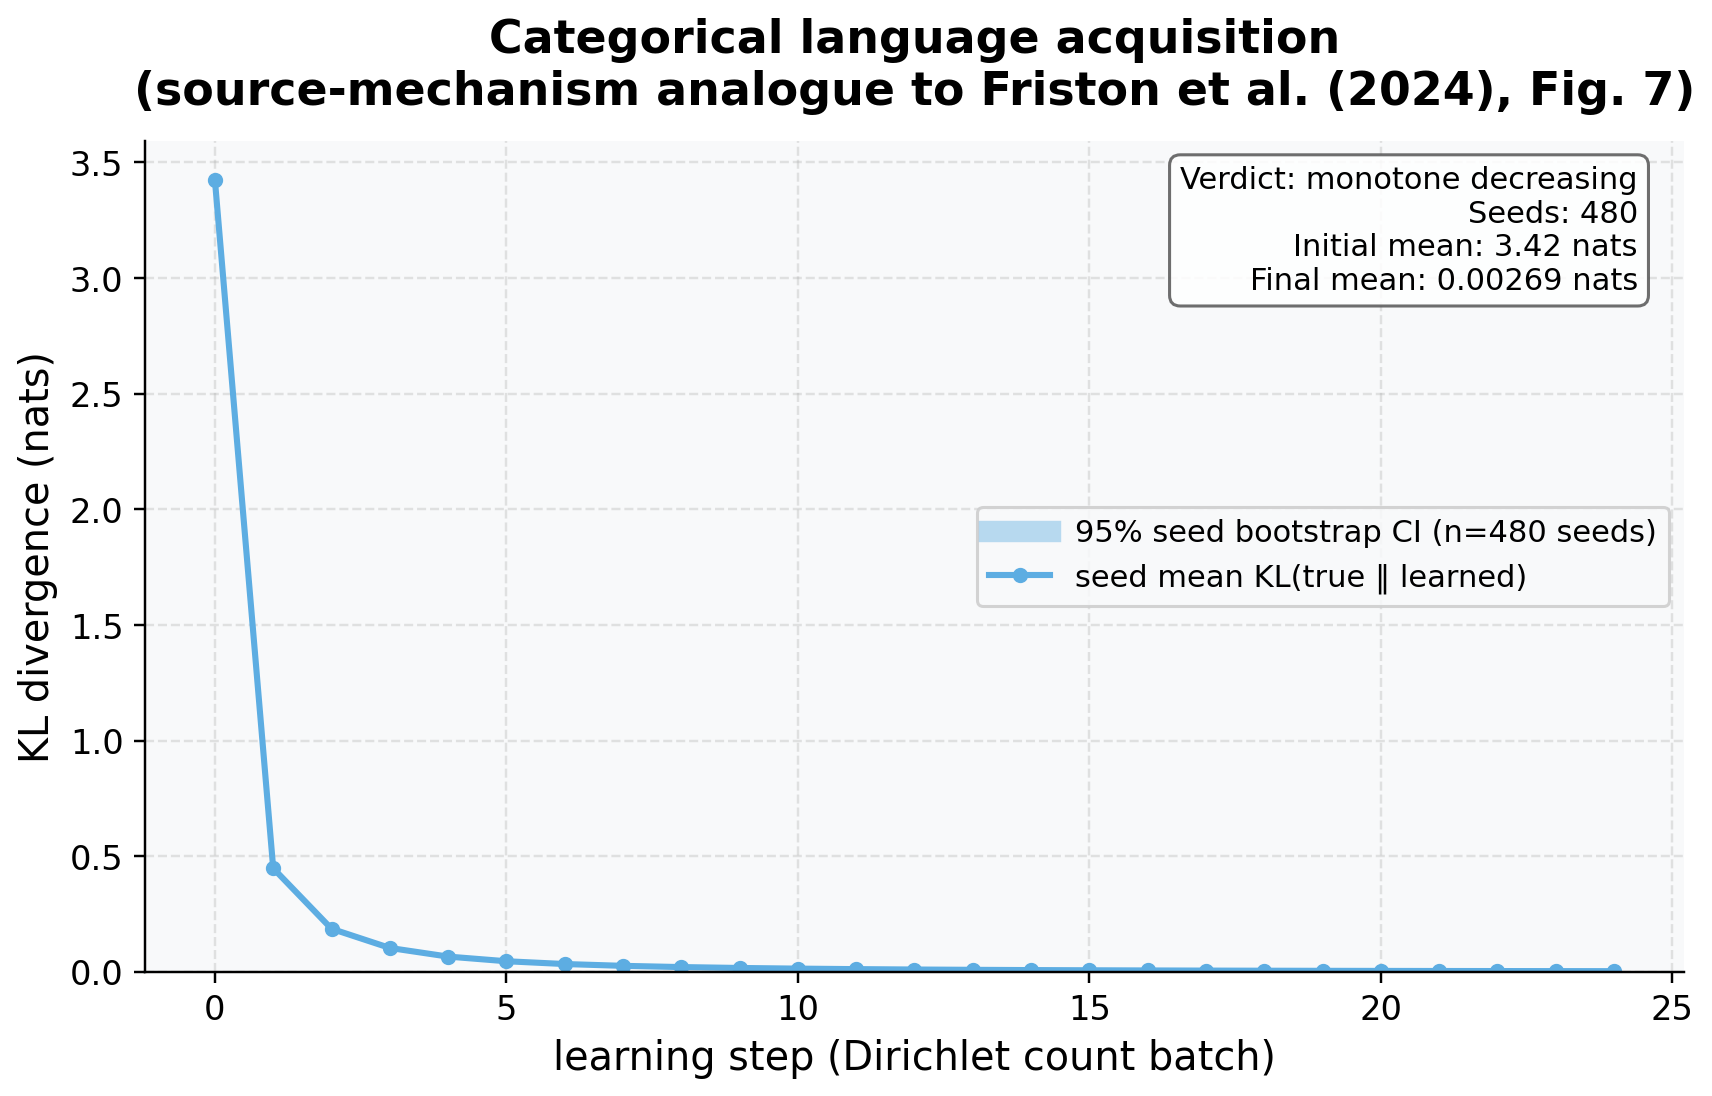
\includegraphics[width=0.8\linewidth,height=0.5\textheight,keepaspectratio,alt={Seed-mean KL divergence from the true categorical likelihood to the learned likelihood across ordered learning batches. The curve decreases rapidly and then approaches zero, with a seed-bootstrap interval band.}]{../figures/language_kl_decay.png}
\caption{Seed-mean KL divergence from the true likelihood A to the
learned likelihood A. The plotted quantity is
\(\mathrm{KL}(\text{true }A \,\|\, \text{learned }A)\). Source relation:
source-mechanism analogue to Friston et al. (2024), Fig. 7; estimand:
seed-mean KL in nats by ordered learning step. The x-axis is the ordered
Dirichlet count batch, from the flat prior at zero through all 24
batches (25 points per seed); the y-axis is summed per-column KL
divergence between the true likelihood and the current expected
likelihood, in nats. The solid line is the mean over 480 independent
configured seeds, and the shaded band is the pointwise 95\%
percentile-bootstrap interval resampling seeds at each learning step.
The replication unit is seed, not the ordered trajectory points. The
mean curve falls monotonically from 3.4231 nats to 0.0027 nats (total
reduction 3.4204 nats, computed from the unrounded endpoints); the
computed monotone-decreasing check is Yes. This reduced categorical
protocol is related to, but does not exactly reproduce, the richer
multi-episode protocol in Friston et al. (2024).}\label{fig:language-kl}
\end{figure}

fig.~\ref{fig:language-kl} plots the full learning curve and its CI
band.

\subsection{Configured BMR sign control
passed}\label{sec:results-emergence}

The first two studies fixed the model structure. This third study
instead checks the sign of a configured Bayesian-model-reduction
comparison. Its estimand is the BMR free-energy difference for two
candidate likelihood-column prunings. The categorical diagnostic is
related to the model-reduction mechanism discussed by Friston et al.
\citep{friston2024federated} and the post-hoc BMR lineage
\citep{friston2011post}. It is not a discovery claim about structure
emergence.

The fixed posterior ranges over \(n = 4\) candidate states. One
likelihood column is unsupported by the configured evidence; another is
a supported control. BMR substitutes a reduced prior for each candidate
and computes \(\Delta F\) eq.~\ref{eq:bmr-deltaf}. This is one
deterministic closed-form comparison, so no resampled sample, confidence
interval, or paired test applies \citep{smith2020active}.

\(\Delta F\) is positive for the declared redundant-column pruning, so
the reduced candidate is favored for this fixed posterior.
\textbf{Redundant-column result:} \(\Delta F=3.68\); the configured
reduction is accepted.

It is negative for the declared supported-column control.
\textbf{Supported-column control:} \(\Delta F=-27.67\); that reduction
is rejected.

\textbf{Configured sign-control disposition:} redundant accepted and
supported rejected, recorded as Yes.

The observed sign pattern
\(\Delta F_{\text{redundant}} > 0 > \Delta F_{\text{supported}}\) passes
the configured control: this fixed posterior favors pruning the declared
redundant column and rejects pruning the declared supported column. It
does not show that arbitrary data or model families will discover,
prune, or retain the correct structure.

\begin{figure}
\centering
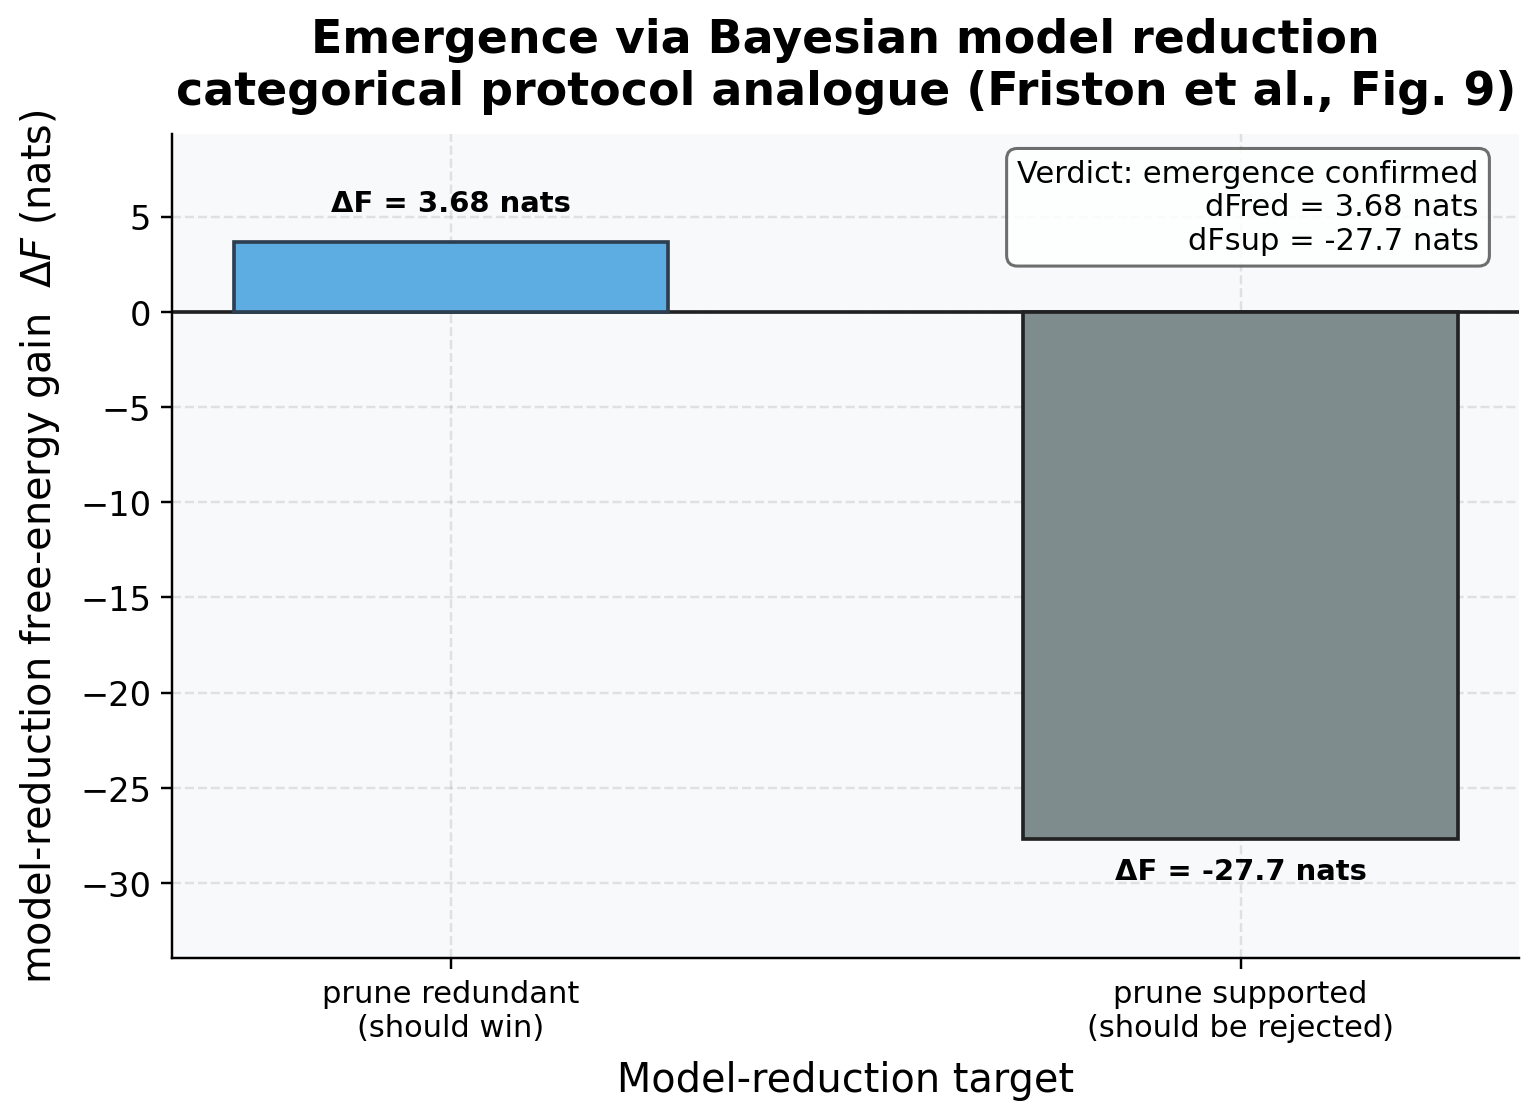
\includegraphics[width=0.8\linewidth,height=0.5\textheight,keepaspectratio,alt={Dotted- and cross-hatched bars show Bayesian model-reduction free-energy differences for pruning a redundant versus supported likelihood column. Direct signed labels and a dotted zero rule show that the configured redundant-pruning control is positive and supported-column pruning is negative.}]{../figures/emergence_bmr.png}
\caption{Configured Bayesian-model-reduction sign control. Source
relation: source-mechanism analogue to the model-reduction mechanism in
Friston et al.~(2024), Fig. 9; estimand: BMR \(\Delta F\) in nats for
two declared pruning candidates. The x-axis is candidate
likelihood-column pruning, ordered as the redundant column and
supported-column control; the y-axis is \(\Delta F\), where positive
values favor the reduced model and negative values reject it. Dotted
hatching and a dark teal keyline identify the favored redundant-column
control, while cross-hatching and a dark neutral keyline identify
rejected supported-column pruning; direct signed value labels and a dark
dotted zero rule duplicate color. On the fixed posterior,
redundant-column pruning gives \(\Delta F = 3.68\) and supported-column
pruning gives \(\Delta F = -27.67\), so the configured sign control
passes (Yes). This is one deterministic closed-form comparison with no
independent replication unit, resampling interval, confidence interval,
or error bar. The configured signs do not establish universal structure
emergence, consistent recovery of true structure, or exact reproduction
of the source simulation.}\label{fig:emergence-bmr}
\end{figure}

fig.~\ref{fig:emergence-bmr} contrasts the two configured prunings and
reports the sign control.

Studies 1--3 all ran in a \emph{trusting} world, where every broadcast
belief is honest. The contamination sweep that follows removes that
assumption, and it is the point at which the three robustness axes of
sec.~\ref{sec:robustness-axes-results} begin to diverge.

\subsection{Contamination sweep: regime-dependent server behavior under
declared attacks}\label{sec:results-robustness}

This experiment compares server presets in one active-inference colony.
Its legacy labels borrow FedGVI client-divergence vocabulary
\citep{mildner2025fedgvi}, but the presets are not client losses or
divergence theorems. \texttt{KLD} denotes the standard log-linear pool;
every other label denotes a \breaktt{robust\_aggregate} heuristic
constant in KLD (c=0.00), RKL (c=1.50), AR (c=1.30), beta (c=1.70), rcce
(c=1.60). The estimand is consensus mass \(q(\text{true state})\) under
the declared contamination mechanism.

The colony contains 7 sentinels, of which 2 mix their broadcasts toward
a confident-wrong delta at each contamination rate. The comparisons
remain conditional on this fixed world, attack target, and preset grid.

The evidence map in fig.~\ref{fig:evidence-replication-map} locates
these comparisons in the conditional heuristic-server lane. It keeps the
fixed-world matched trials distinct from the seed-level review below and
prevents either result from inheriting client-loss or variational-server
guarantees.

As the contamination rate rises across
\(\{0, 0.225, 0.45, 0.675, 0.9\}\), the \textbf{standard} (\texttt{KLD})
consensus accuracy degrades monotonically:

\begin{longtable}[]{@{}llllll@{}}
\caption{Consensus accuracy \(q(\text{true state})\) by contamination
rate and configured server operating point (\(n = 1\) deterministic
sweep per cell). \protect\texttt{KLD} is the standard log-linear pool
(eq.~\ref{eq:log-linear-pool}); the other columns use the fixed
heuristic constants listed above in the same seeded colony. This table
is descriptive; inferential paired evidence appears
below.}\label{tbl:robustness_sweep}\tabularnewline
\toprule\noalign{}
Contamination rate & KLD & RKL & AR & beta & rcce \\
\midrule\noalign{}
\endfirsthead
\toprule\noalign{}
Contamination rate & KLD & RKL & AR & beta & rcce \\
\midrule\noalign{}
\endhead
\bottomrule\noalign{}
\endlastfoot
0 & 1.000 & 0.997 & 0.998 & 0.996 & 0.996 \\
0.225 & 0.999 & 0.993 & 0.995 & 0.990 & 0.992 \\
0.45 & 0.995 & 0.987 & 0.990 & 0.984 & 0.986 \\
0.675 & 0.975 & 0.985 & 0.989 & 0.981 & 0.983 \\
0.9 & 0.693 & 0.984 & 0.988 & 0.980 & 0.982 \\
\end{longtable}

As the saboteurs capture more belief mass, \texttt{KLD} falls
monotonically while at least one non-reference preset remains above the
stated accuracy threshold. \textbf{Reference trend:} standard accuracy
degrades monotonically with rate, recorded as Yes.

\textbf{Worst-rate display check:} at rate 0.900, at least one
non-reference preset remains at or above 0.50, recorded as Yes. Standard
accuracy is 0.6928; the highest robust consensus mass in this
single-world mechanistic sweep is 0.9880, attained by AR.

The rate trend above is one deterministic sweep per cell. The paired
profile reruns each rate over \(n_{\rm trial} = 960\) matched trials
nested within the fixed seeded world. Each non-reference preset is
compared with the standard pool, and p-values are BH-adjusted within
method \citep{benjamini1995controlling}. This is a finite, rate-resolved
diagnostic, not a continuous-family result.

\begin{longtable}[]{@{}llll@{}}
\caption{Effect-size projection of the per-contamination-rate
standard-versus-preset paired tests, keyed by
\protect\breaktt{(server\ preset,\ rate)}. Each cell uses 960 matched
trial replicates nested within the fixed seeded world. Joining this
projection to tbl.~\ref{tbl:paired-by-rate-inference} on the displayed
key reconstructs every source row exactly; the label and
\(d\)-equivalent do not add an independent world-level
estimand.}\label{tbl:paired-by-rate}\tabularnewline
\toprule\noalign{}
Server preset & Rate & Rank-biserial-derived \(d\)-equivalent & Label \\
\midrule\noalign{}
\endfirsthead
\toprule\noalign{}
Server preset & Rate & Rank-biserial-derived \(d\)-equivalent & Label \\
\midrule\noalign{}
\endhead
\bottomrule\noalign{}
\endlastfoot
RKL & 0 & saturated (r=-1) & large \\
RKL & 0.225 & saturated (r=-1) & large \\
RKL & 0.45 & saturated (r=-1) & large \\
RKL & 0.675 & 13.79 & large \\
RKL & 0.9 & -0.37 & small \\
AR & 0 & saturated (r=-1) & large \\
AR & 0.225 & saturated (r=-1) & large \\
AR & 0.45 & -303.73 & large \\
AR & 0.675 & 160.07 & large \\
AR & 0.9 & -1.57 & large \\
beta & 0 & saturated (r=-1) & large \\
beta & 0.225 & saturated (r=-1) & large \\
beta & 0.45 & saturated (r=-1) & large \\
beta & 0.675 & 2.81 & large \\
beta & 0.9 & 0.61 & medium \\
rcce & 0 & saturated (r=-1) & large \\
rcce & 0.225 & saturated (r=-1) & large \\
rcce & 0.45 & saturated (r=-1) & large \\
rcce & 0.675 & 5.67 & large \\
rcce & 0.9 & 0.14 & negligible \\
\end{longtable}

\begin{longtable}[]{@{}lllll@{}}
\caption{Inference projection of the same per-rate matched-pairs
Wilcoxon tests \citep{wilcoxon1945individual, fay2010wilcoxon}, keyed by
\protect\breaktt{(server\ preset,\ rate)} and BH-deflated within each
preset's rate family. \protect\texttt{Reject} is the report-owned family
decision. The 960 trials are nested within one fixed seeded world, not
960 independent worlds; this table must be read with
tbl.~\ref{tbl:paired-by-rate} to recover the complete source
row.}\label{tbl:paired-by-rate-inference}\tabularnewline
\toprule\noalign{}
Server preset & Rate & Raw p & q & Reject \\
\midrule\noalign{}
\endfirsthead
\toprule\noalign{}
Server preset & Rate & Raw p & q & Reject \\
\midrule\noalign{}
\endhead
\bottomrule\noalign{}
\endlastfoot
RKL & 0 & 1.11e-158 & 1.85e-158 & Yes \\
RKL & 0.225 & 1.11e-158 & 1.85e-158 & Yes \\
RKL & 0.45 & 1.11e-158 & 1.85e-158 & Yes \\
RKL & 0.675 & 1.88e-155 & 2.35e-155 & Yes \\
RKL & 0.9 & 1.06e-06 & 1.06e-06 & Yes \\
AR & 0 & 1.11e-158 & 1.47e-158 & Yes \\
AR & 0.225 & 1.11e-158 & 1.47e-158 & Yes \\
AR & 0.45 & 1.13e-158 & 1.47e-158 & Yes \\
AR & 0.675 & 1.17e-158 & 1.47e-158 & Yes \\
AR & 0.9 & 1.62e-61 & 1.62e-61 & Yes \\
beta & 0 & 1.11e-158 & 1.85e-158 & Yes \\
beta & 0.225 & 1.11e-158 & 1.85e-158 & Yes \\
beta & 0.45 & 1.11e-158 & 1.85e-158 & Yes \\
beta & 0.675 & 6.29e-106 & 7.86e-106 & Yes \\
beta & 0.9 & 6.04e-15 & 6.04e-15 & Yes \\
rcce & 0 & 1.11e-158 & 1.85e-158 & Yes \\
rcce & 0.225 & 1.11e-158 & 1.85e-158 & Yes \\
rcce & 0.45 & 1.11e-158 & 1.85e-158 & Yes \\
rcce & 0.675 & 2.37e-141 & 2.96e-141 & Yes \\
rcce & 0.9 & 6.54e-02 & 6.54e-02 & No \\
\end{longtable}

The \texttt{KLD} baseline is excluded from both projections because it
is the standard reference, not a self-contrast. The displayed
\(d\)-equivalent is a rank-biserial-derived transform, not raw Cohen's
\(d\); the signed-saturation marker flags contrasts where the
rank-biserial correlation saturates at \(\pm1\). These contrasts
decorate the server-side \breaktt{robust\_aggregate} heuristic only.

\begin{figure}
\centering
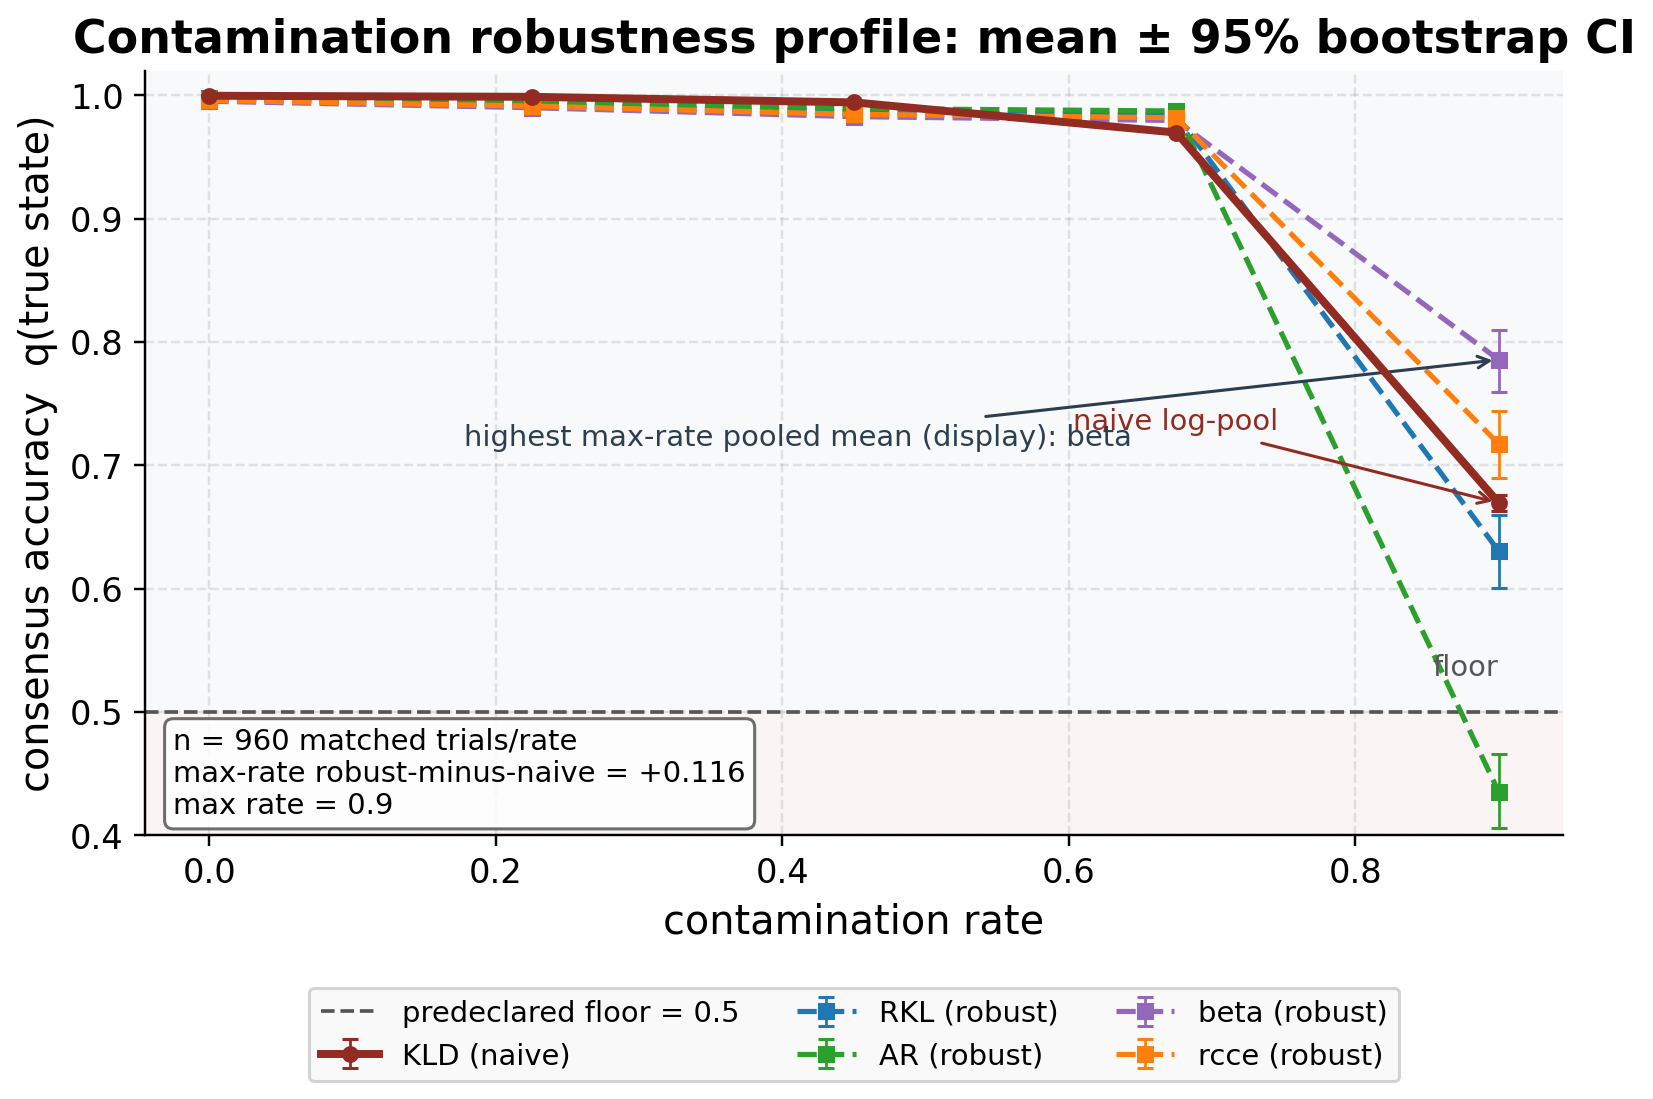
\includegraphics[width=0.8\linewidth,height=0.5\textheight,keepaspectratio,alt={Consensus true-state-mass curves compare the standard log-linear pool with four actual robust-aggregate server presets. Distinct markers and dashes show matched-trial means with 95-percent percentile-bootstrap intervals; the horizontal rule is the declared accuracy floor.}]{../figures/robustness_sweep.png}
\caption{Consensus accuracy: probability mass assigned to the true
hidden state. The plotted estimand is \(q(\text{true state})\). Source
relation: original project robustness extension; estimand: true-state
probability mass; uncertainty: matched-trial percentile-bootstrap
intervals over configured trials. The x-axis is saboteur convex-mix
contamination rate over \(\{0, 0.225, 0.45, 0.675, 0.9\}\); the y-axis
is consensus probability mass on the true state. Curves compare the
standard \protect\texttt{KLD} log-linear pool with
\protect\breaktt{robust\_aggregate} server presets
\(KLD (c=0.00), RKL (c=1.50), AR (c=1.30), beta (c=1.70), rcce (c=1.60)\)
for \(7\) agents, including \(2\) saboteurs; they are not named client
losses. Distinct markers, dashes, direct labels, and the dark dotted
threshold at 0.50 duplicate color. The independent replication unit is a
matched synthetic trial within the fixed seeded true state and attack
target, with 960 trials per rate. Curves show trial means with 95\%
percentile-bootstrap confidence intervals. At the largest rate, the
standard pool reaches 0.6697 and the within-sweep highest pooled robust
mean reaches 0.7857. That operating point is a disclosed display
selection: low-rate robust means can match or trail the standard pool,
and individual presets can fall below the threshold. The truncated
linear y-axis enlarges the declared threshold region. This fixed-world
sweep does not establish a universal method ranking, alternate-world
generalization, a client-loss theorem, bounded influence, or Byzantine
tolerance; the selection-free seed-level review is reported
separately.}\label{fig:robustness-sweep}
\end{figure}

\subsubsection{Selection-free all-method robustness
review}\label{sec:results-review-grid}

The comparison in fig.~\ref{fig:robustness-review-grid} is the principal
comparative robustness surface. It joins the conditional-world cells to
the directional rate profiles while retaining every configured
non-reference server preset. It uses 160 deterministic seed replicates
and 24 trials nested within each seed and cell.

Read the portrait surface from top to bottom: Panel A is the full-width
conditional heatmap, and Panels B--D stack the three rate profiles.
Their elbow leaders terminate in reserved right-side label lanes so
curve identity remains separate from the plotted endpoints.

The finite attack union is clean, confident wrong, permutation,
byzantine, drift, label noise, uniform. The rate-resolved directional
mechanisms are confident wrong, byzantine, drift, with entropy controls
uniform, label noise and registered rates
\(\{0, 0.2, 0.4, 0.5, 0.6, 0.7, 0.8, 0.9\}\). The independent unit is
seed within a declared scenario or rate cell; the nesting rule is
n\_trials nested within each seed/cell; no trial is promoted to an
independent world.

The payload is selection-free source payload; every configured non-KLD
method is reported at every directional rate and no winner is used for
inference, and its statistics surface is selection-free. It retains
seed-level contrasts, paired Wilcoxon/rank-biserial results,
percentile-bootstrap intervals, MCSE, an observed-effect MDE, and
BH-adjusted rate families. BH ownership is BH is applied within each
attack-mechanism \texorpdfstring{\ensuremath{\times}}{x} method rate family; cells sharing design structure
are not treated as independent families.

The precision plan targets maximum MCSE 0.0100; the observed maximum is
0.0066 across 96. No method is selected by seed, rate, or pooled mean.
Mixed and reversed cells remain visible, and the grid does not close the
open calibration, external-data, or server-theory questions.

The source-generated exact-value fallback calls the same finite grouping
helper as Panel A. For every displayed attack-by-weight cell it records
the printed grouped mean and the printed half min--max span, preventing
the numeric fallback from drifting from the renderer.

\begin{figure}
\centering
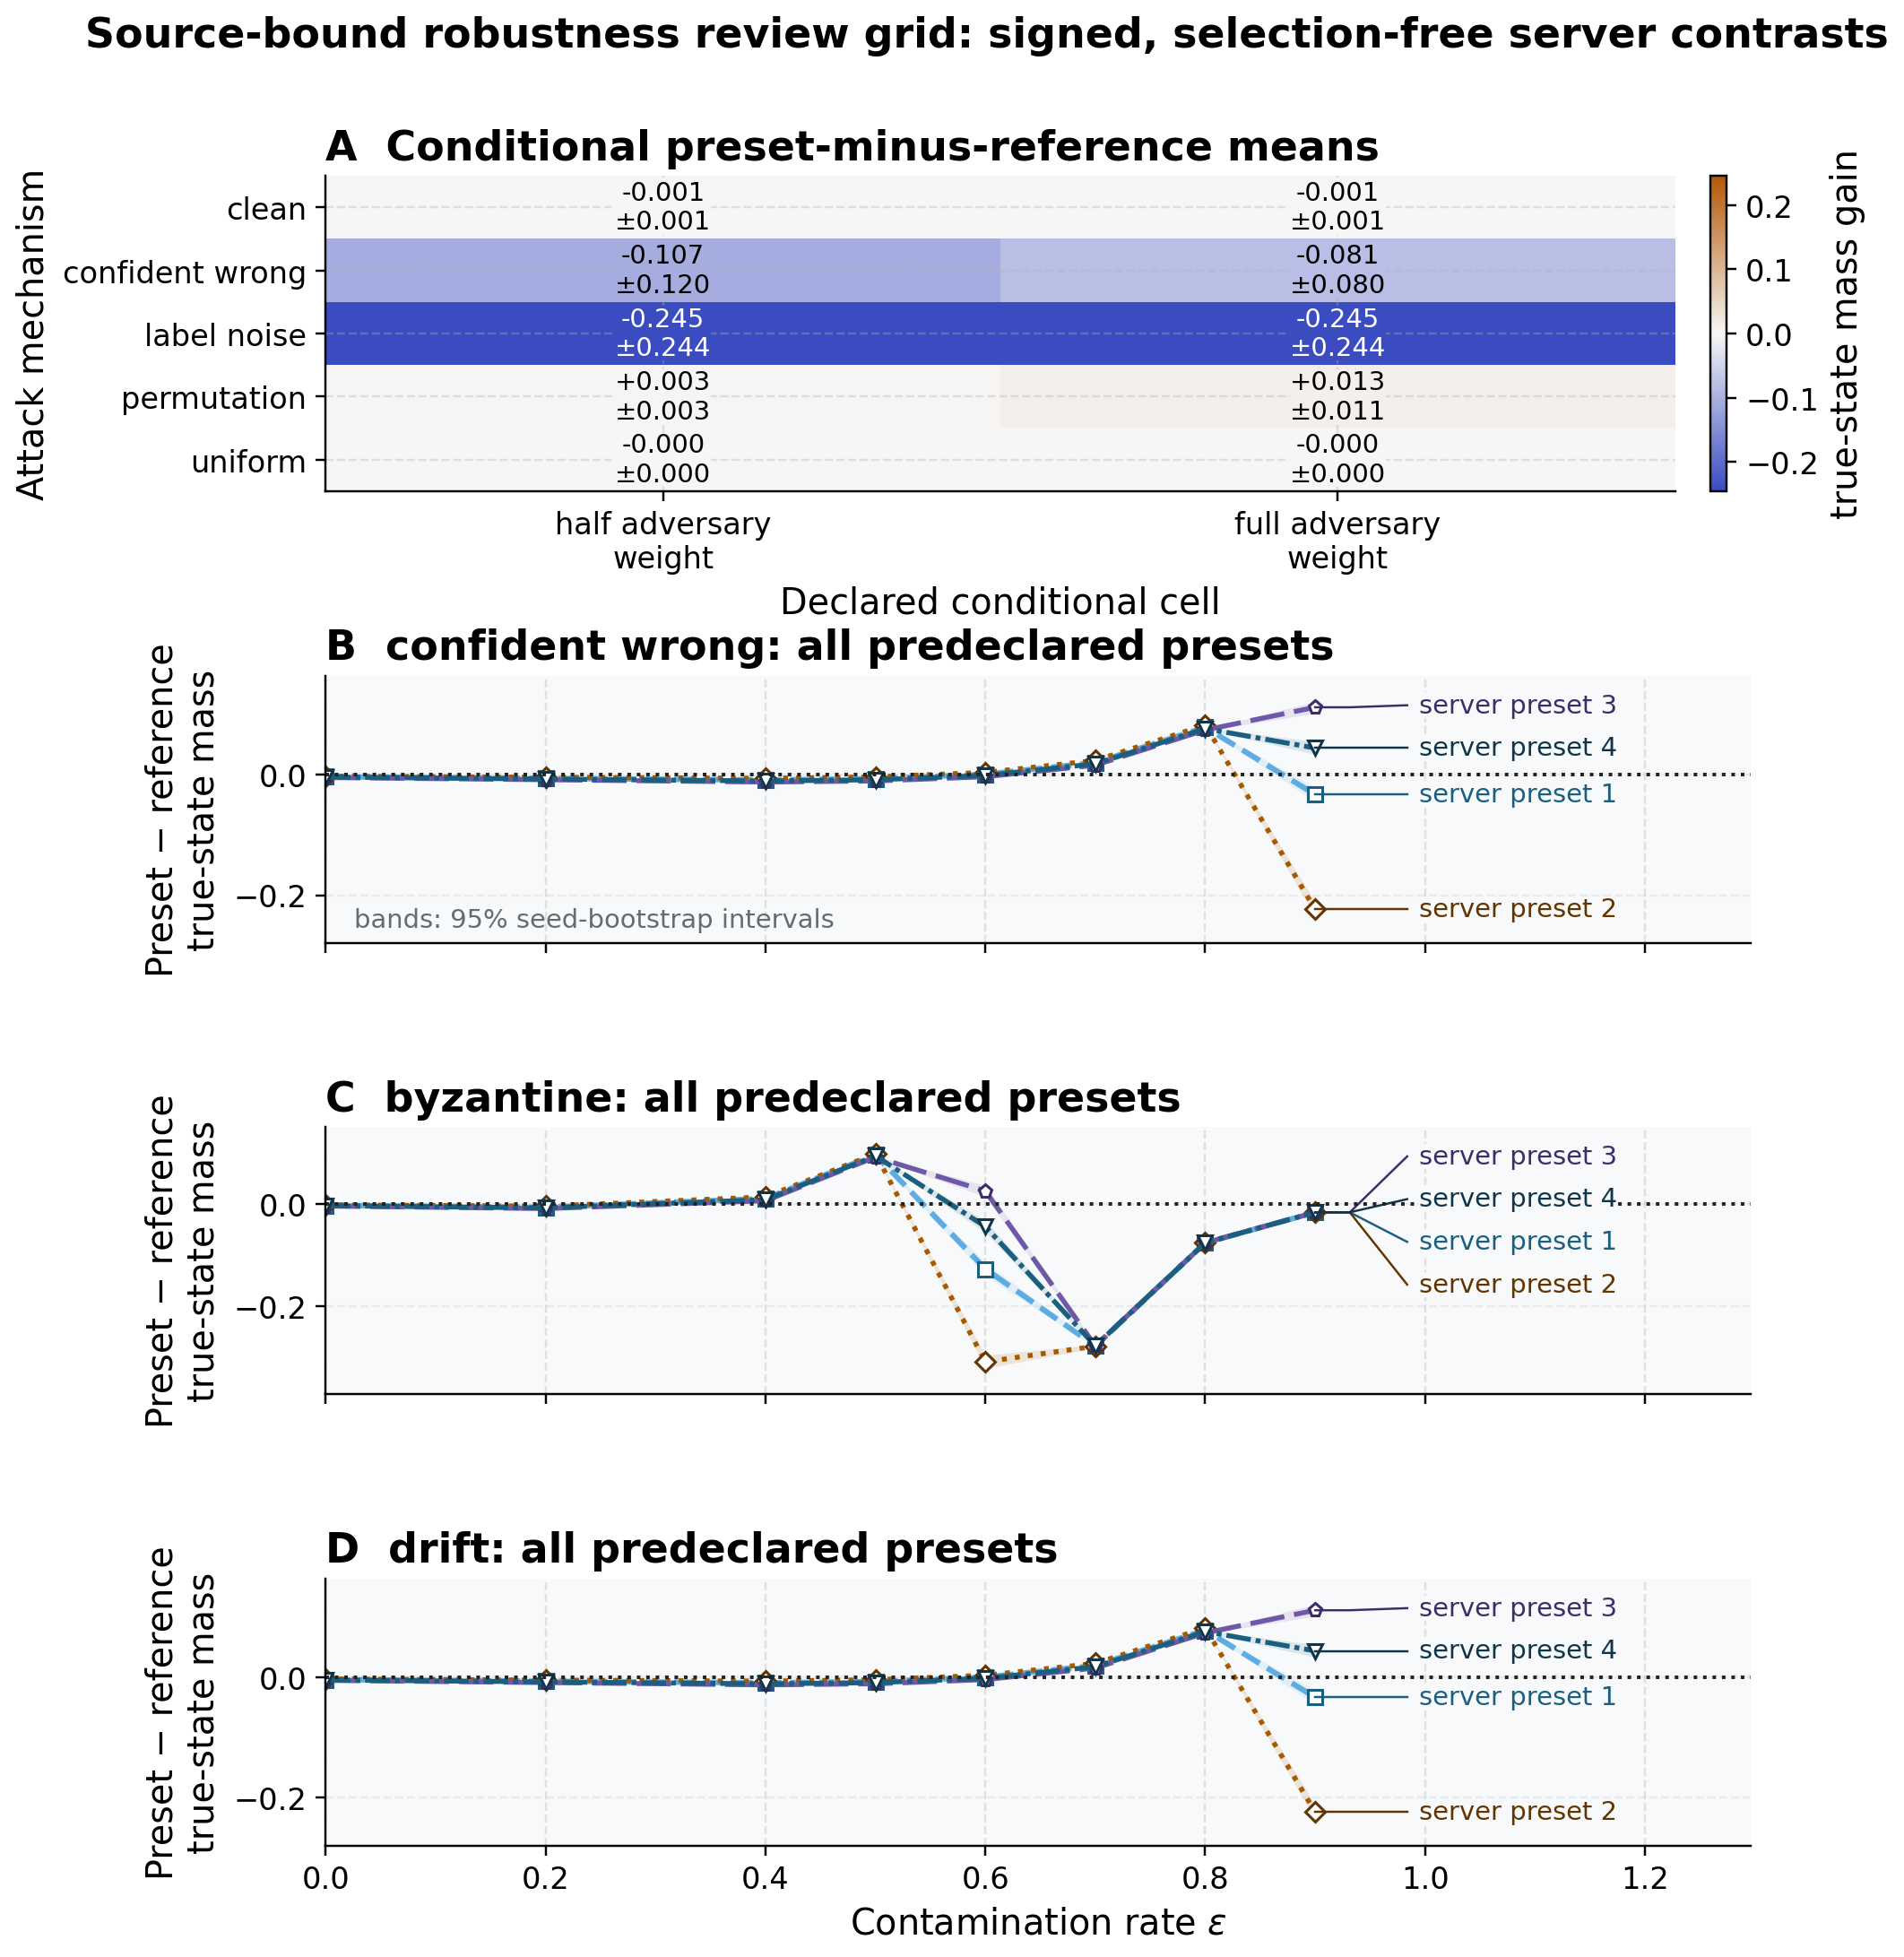
\includegraphics[width=0.98\linewidth,height=0.5\textheight,keepaspectratio,alt={Portrait robustness review with a full-width top heatmap and three rate profiles stacked below for confident-wrong, Byzantine, and drift attacks. Every predeclared server preset uses a distinct marker and dash; elbow leaders route endpoints into a dedicated right label lane. Heatmap second lines are finite-grid spans, not confidence intervals.}]{../figures/robustness_review_grid.png}
\caption{The robustness review retains every server preset and preserves
mixed signs across the attack grid. Source relation: original project
conditional simulation review joining registered conditional-world and
directional-rate reports; study status: selection-free, all-method
finite-grid evidence; estimand: seed-level robust-minus-standard
true-state probability-mass contrast. Read the portrait figure from top
to bottom: Panel A is a full-width heatmap of conditional attack cells
by adversarial-weight setting; Panels B--D stack confident-wrong,
Byzantine, and drift rate profiles. The x-axis is adversarial weight in
Panel A and contamination rate in Panels B--D; the y-axis is contrast in
probability units. Printed cell signs, distinct markers and dashes, and
elbow leaders into reserved right-side endpoint-label lanes duplicate
color; the dark dotted rule marks zero. The independent replication unit
is the configured seed (\(n=160\)), with 24 trials plus agents and
conditions nested within each cell. Rate-profile bands are 95\%
percentile-bootstrap intervals over seeds. The second heatmap line is
half the finite-grid min--max span, not a confidence interval. No curve
is selected by pooled mean. The figure supports only mechanism- and
grid-conditional contrasts; it does not establish a universal winner,
bounded influence, Byzantine tolerance, a causal effect, independent
shared-design cells, or generalization beyond the registered
worlds.}\label{fig:robustness-review-grid}
\end{figure}

\subsubsection{Conditional matched-trial comparison at the declared
rate}\label{sec:results-verdict}

At contamination rate 0.800, each of 960 matched trials redraws the
heterogeneous healthy colony while holding the seeded world's true state
and attack target fixed. Each non-reference server preset is compared
with the standard pool using the paired Wilcoxon signed-rank test
\citep{wilcoxon1945individual}. Benjamini--Hochberg FDR adjustment
applies within the declared family \citep{benjamini1995controlling}.

The generated \texttt{Wins} field is true only when the adjusted null is
rejected and the paired effect is positive. It is conditional
bookkeeping for this fixed world and rate, not a universal method
ranking.

\begin{longtable}[]{@{}lllll@{}}
\caption{Per-preset paired comparison against the standard pool at rate
0.800 (\(n_{\rm trial} = 960\) matched trial replicates, signed-rank
test under the paired-difference assumptions of
sec.~\ref{sec:methods-paired}). This is a fixed-world conditional
diagnostic; seed-level inference is reported separately in
sec.~\ref{sec:results-review-grid}. Effect size is the matched-pairs
rank-biserial correlation; positive values mean the non-reference preset
exceeds the standard pool. A \protect\texttt{Wins} value is true only
when the BH-adjusted null is rejected \emph{and} the effect is positive,
with FDR scoped to this declared
family.}\label{tbl:robustness_verdict}\tabularnewline
\toprule\noalign{}
Server preset & Effect size & Raw p & q & Wins \\
\midrule\noalign{}
\endfirsthead
\toprule\noalign{}
Server preset & Effect size & Raw p & q & Wins \\
\midrule\noalign{}
\endhead
\bottomrule\noalign{}
\endlastfoot
AR & 1.0000 & 1.11e-158 & 1.11e-158 & Yes \\
RKL & 1.0000 & 1.11e-158 & 1.11e-158 & Yes \\
beta & 1.0000 & 1.11e-158 & 1.11e-158 & Yes \\
rcce & 1.0000 & 1.11e-158 & 1.11e-158 & Yes \\
\end{longtable}

\begin{longtable}[]{@{}
  >{\raggedright\arraybackslash}p{(\linewidth - 8\tabcolsep) * \real{0.2000}}
  >{\raggedright\arraybackslash}p{(\linewidth - 8\tabcolsep) * \real{0.2000}}
  >{\raggedright\arraybackslash}p{(\linewidth - 8\tabcolsep) * \real{0.2000}}
  >{\raggedright\arraybackslash}p{(\linewidth - 8\tabcolsep) * \real{0.2000}}
  >{\raggedright\arraybackslash}p{(\linewidth - 8\tabcolsep) * \real{0.2000}}@{}}
\caption{Effect estimates at rate 0.800 (\(n_{\rm trial} = 960\) matched
trial replicates). Source relation and study status: these rows are
generated from the typed primary-sweep report and constitute a
conditional fixed-world diagnostic. Each row gives the
rank-biserial-derived \(d\)-equivalent and display label, followed by
the mean non-reference-minus-standard accuracy difference in
accuracy-proportion units and its 95\% percentile-bootstrap CI. The
matched trial is the resampling unit; all trials remain nested within
the one seeded world. Row order is preserved in
tbl.~\ref{tbl:verdict-inference-power}. The signed-saturation marker
replaces a misleading finite literal where the rank-biserial transform
diverges. These estimates do not identify an independently replicated
world effect, calibration result, or universal server
ranking.}\label{tbl:verdict-effect-estimates}\tabularnewline
\toprule\noalign{}
\begin{minipage}[b]{\linewidth}\raggedright
Method
\end{minipage} & \begin{minipage}[b]{\linewidth}\raggedright
Derived \(d_{\rm eq}\)
\end{minipage} & \begin{minipage}[b]{\linewidth}\raggedright
Label
\end{minipage} & \begin{minipage}[b]{\linewidth}\raggedright
Mean \(\Delta\) accuracy
\end{minipage} & \begin{minipage}[b]{\linewidth}\raggedright
95\% CI
\end{minipage} \\
\midrule\noalign{}
\endfirsthead
\toprule\noalign{}
\begin{minipage}[b]{\linewidth}\raggedright
Method
\end{minipage} & \begin{minipage}[b]{\linewidth}\raggedright
Derived \(d_{\rm eq}\)
\end{minipage} & \begin{minipage}[b]{\linewidth}\raggedright
Label
\end{minipage} & \begin{minipage}[b]{\linewidth}\raggedright
Mean \(\Delta\) accuracy
\end{minipage} & \begin{minipage}[b]{\linewidth}\raggedright
95\% CI
\end{minipage} \\
\midrule\noalign{}
\endhead
\bottomrule\noalign{}
\endlastfoot
AR & saturated (r=+1) & large & 0.0846 & {[}0.0821, 0.0873{]} \\
RKL & saturated (r=+1) & large & 0.0809 & {[}0.0783, 0.0834{]} \\
beta & saturated (r=+1) & large & 0.0764 & {[}0.0738, 0.0790{]} \\
rcce & saturated (r=+1) & large & 0.0787 & {[}0.0761, 0.0814{]} \\
\end{longtable}

\begin{longtable}[]{@{}llllll@{}}
\caption{Inference and planning diagnostics for the same ordered method
rows and matched trials as tbl.~\ref{tbl:verdict-effect-estimates}.
Source relation and study status: the typed primary-sweep report
supplies every cell for this conditional fixed-world comparison. Raw
paired-Wilcoxon p-values are accompanied by BH-deflated q-values and the
resulting rejection indicator for the declared method family.
Observed-effect design power uses \(\alpha = 0.05\) and alternative
\protect\texttt{greater}; the prospective \(n_{\rm trial}\) targets
power 0.80. The matched trial is the inferential and planning unit
within one seeded world. Power and target sample size are conditional
approximations derived from the observed effect, not independent
confirmation, calibration, a guarantee of future power, or evidence
beyond the declared world and
rate.}\label{tbl:verdict-inference-power}\tabularnewline
\toprule\noalign{}
Method & Raw p & q & Power & Target \(n_{\rm trial}\) & Reject \\
\midrule\noalign{}
\endfirsthead
\toprule\noalign{}
Method & Raw p & q & Power & Target \(n_{\rm trial}\) & Reject \\
\midrule\noalign{}
\endhead
\bottomrule\noalign{}
\endlastfoot
AR & 1.11e-158 & 1.11e-158 & 1.0000 & 5 & Yes \\
RKL & 1.11e-158 & 1.11e-158 & 1.0000 & 5 & Yes \\
beta & 1.11e-158 & 1.11e-158 & 1.0000 & 5 & Yes \\
rcce & 1.11e-158 & 1.11e-158 & 1.0000 & 5 & Yes \\
\end{longtable}

\begin{longtable}[]{@{}llll@{}}
\caption{Per-method consensus accuracy at the verdict rate 0.800 with
95\% percentile-bootstrap CI, including the standard
\protect\texttt{KLD} baseline. The CI is conditional on the seeded
matched-trial design and resamples trials, not alternate world models.
The standard pool sits at 0.9021 (\([0.8993, 0.9049]\)); the headline
display method RKL has pooled mean 0.9829
(\([0.9827, 0.9832]\)).}\label{tbl:accuracy-at-verdict}\tabularnewline
\toprule\noalign{}
Method & n & Mean acc. @ verdict rate & 95\% CI \\
\midrule\noalign{}
\endfirsthead
\toprule\noalign{}
Method & n & Mean acc. @ verdict rate & 95\% CI \\
\midrule\noalign{}
\endhead
\bottomrule\noalign{}
\endlastfoot
KLD & 960 & 0.9021 & {[}0.8993, 0.9049{]} \\
RKL & 960 & 0.9829 & {[}0.9827, 0.9832{]} \\
AR & 960 & 0.9867 & {[}0.9865, 0.9869{]} \\
beta & 960 & 0.9785 & {[}0.9782, 0.9787{]} \\
rcce & 960 & 0.9808 & {[}0.9806, 0.9810{]} \\
\end{longtable}

\textbf{Reference mean.} Naive-pool mean accuracy at the verdict rate is
0.9021 (per-trial mean over 960 trials; the bootstrap CI is in
tbl.~\ref{tbl:accuracy-at-verdict}).

\textbf{Positive contrasts.} At least one non-reference preset is a
BH-rejected positive contrast: Yes.

\textbf{Headline display.} The method is RKL (tied set: RKL, AR, beta,
rcce), with rank-biserial-derived \(d\)-equivalent saturated (r=+1)
(large), mean accuracy difference 0.0809 (\([0.0783, 0.0834]\)), raw
\(p = 1.11 \times 10^{-158}\), and \(q = 1.11 \times 10^{-158}\).

Its observed-effect design power is 1.0000. Prospective \(n\) for power
0.80 is 5.

\textbf{Display rule.} Under largest positive rank-biserial
effect\_size; stable method order tie-break (tie-break: first robust
method in divergences order), observed-effect design power is 1.0000 at
the run's \(n_{\rm trial} = 960\). A confirmatory replication should
budget \(n_{\rm trial} = 5\) for power 0.80 (prospective \(n = 7\)).

The standard pool degrades and some non-reference presets have positive
conditional contrasts. The statistics module produces the paired tests,
multiple-testing adjustment, bootstrap intervals, and planning analysis;
the prose does not promote them beyond their matched-trial estimand.

The headline label is a deterministic display choice, not a unique
scientific winner. The complete tied set is RKL, AR, beta, rcce, the
largest paired mean-difference method is AR, and the worst-rate pooled
display method is beta. These may differ because they answer different
descriptive questions.

\paragraph{Server-side heuristic axis: conditional contrasts without
theorem
transfer}\label{server-side-heuristic-axis-conditional-contrasts-without-theorem-transfer}

The comparison above belongs to the heuristic server axis defined in
sec.~\ref{sec:robustness-axes}. fig.~\ref{fig:robust-weights} visualizes
the \breaktt{robust\_aggregate} divergence-reweighting that down-weights
agents at pooling time. Its positive formal property is the
naive-recovery limit of Theorem \ref{thm:belief-sharing-recovery}
(eq.~\ref{eq:robust-identity}, the 0 residual of
sec.~\ref{sec:results-recovery}), and it has a scoped no-go result for a
declared separable objective class, not an objective certificate.

The heuristic carries no bounded-influence guarantee. The effect sizes,
intervals, and planning quantities characterize its conditional
contrasts; they do not certify the per-agent generalized-Bayes claim,
which remains separately source-conditional in
sec.~\ref{sec:results-baseline}.

\begin{figure}
\centering
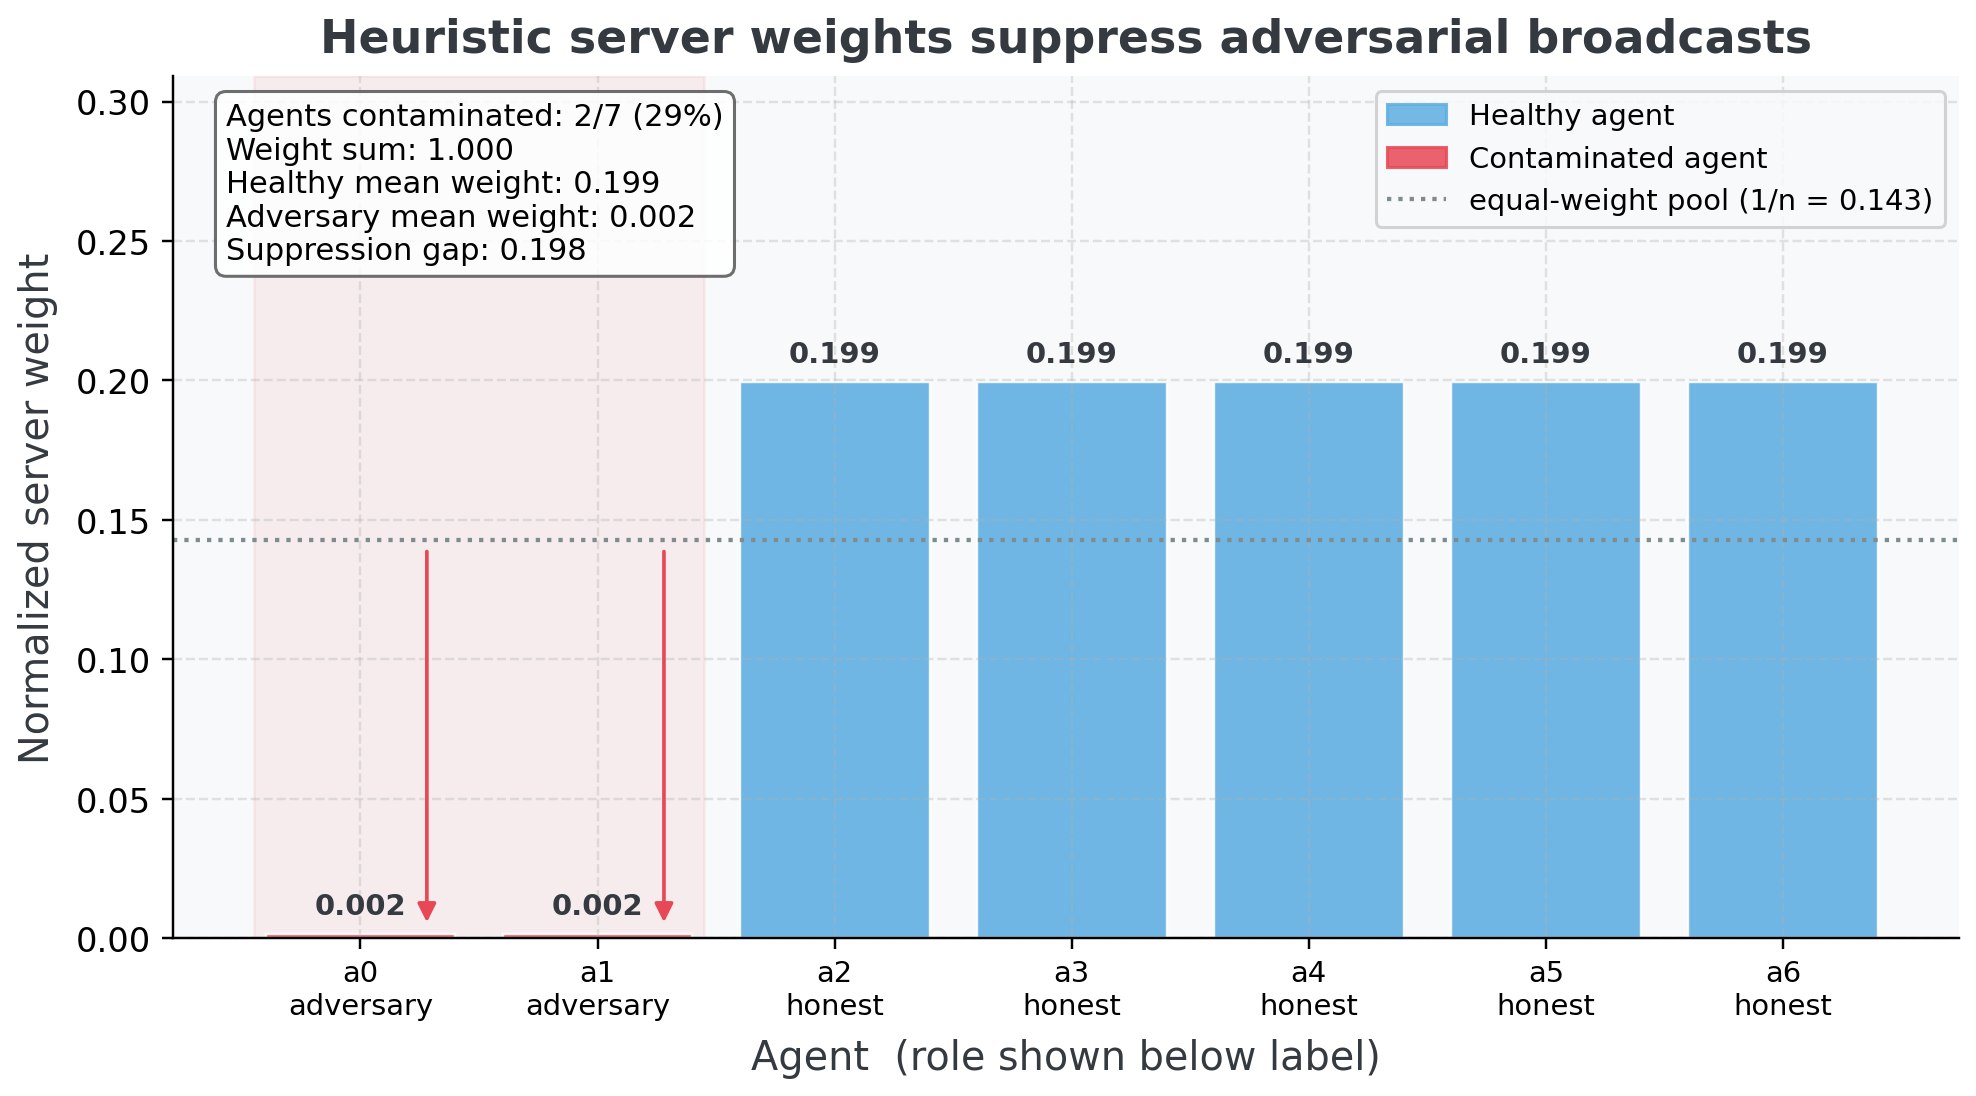
\includegraphics[width=0.8\linewidth,height=0.5\textheight,keepaspectratio,alt={Bar chart of server weights for two contaminated and five honest agents. The heuristic assigns near-zero weight to contaminated broadcasts and larger, near-equal weights to honest agents; the dotted line is equal weight.}]{../figures/robust_influence_weights.png}
\caption{Server-side influence weights assigned by
\protect\breaktt{robust\_aggregate}. Source relation: original project
server-side diagnostic; estimand: normalized pooling weight;
uncertainty: deterministic single-run display. Divergence-reweighting
weights for each of the \(7\) agents at the verdict contamination rate
\(0.800\) (the convex-mix strength applied to each saboteur's belief ---
distinct from the \emph{count} of contaminated agents, \(2\) of \(7\),
reported in the in-figure box). x-axis: agent index, zero-based (\(a0\)
upward), with each agent's role (honest / adversary) shown beneath its
label; y-axis: normalized pooling weight, with weights summing to one
and the dotted reference marking the equal-weight pool (\(1/n\)). The
\(2\) contaminated agents use cross-hatching and direct role labels;
downward arrows mark suppression below the equal-weight reference. No
resampling interval applies to this deterministic run. This
server-heuristic display establishes neither the per-client
bounded-influence theorem, Byzantine tolerance, nor a universal
influence bound.}\label{fig:robust-weights}
\end{figure}

\subsubsection{Variational aggregator: conservative objective-backed
weight control}\label{sec:results-variational}

The heuristic has the higher point accuracy in the configured verdict
cell. The variational aggregator of sec.~\ref{sec:method-variational},
derived in sec.~\ref{sec:supp-variational}, is its objective-backed
complement. Each exact block update does not increase the stated free
energy eq.~\ref{eq:agg-free-energy}, and a converged fixed point is
coordinatewise stationary. Two deterministic runs show its weight
behavior at robustness 1.50.

First, the descent. On a contaminated colony the free energy falls
monotonically from 3.2458 to 2.3780 (a drop of 0.8678 over 11
block-coordinate iterations, converged: Yes), with a largest single-step
\emph{increase} of 8.88e-16 --- machine zero, the numerical witness of
the descent theorem (sec.~\ref{sec:supp-theorem}).

\begin{figure}
\centering
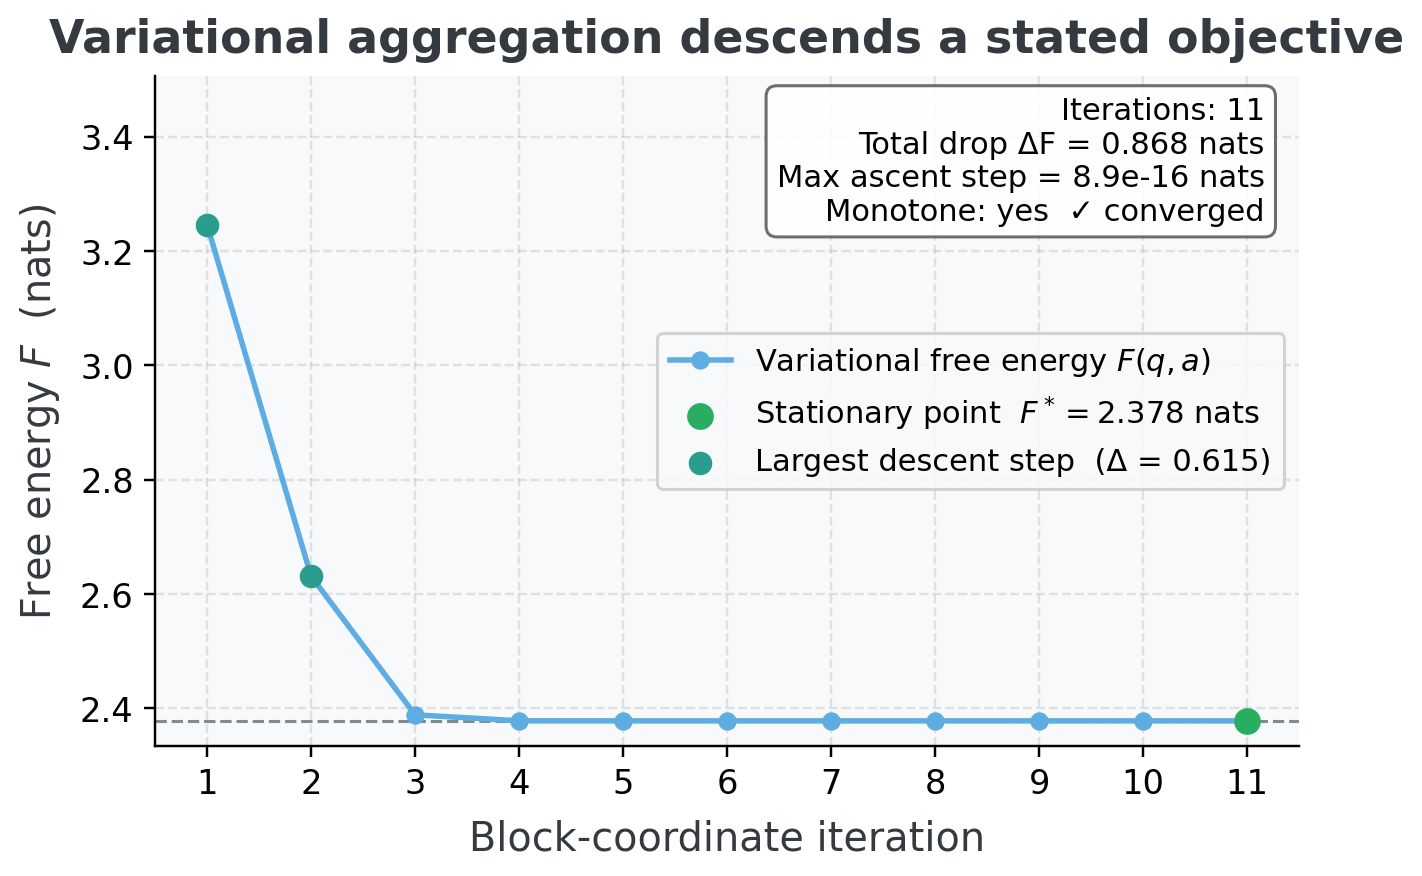
\includegraphics[width=0.8\linewidth,height=0.5\textheight,keepaspectratio,alt={Line plot of variational free energy versus block-coordinate iteration. The trace drops steeply at first, then remains flat through convergence.}]{../figures/aggregation_descent.png}
\caption{Variational free energy \(F(q, a)\) as a function of
block-coordinate descent iteration. Source relation: original project
objective-descent diagnostic; estimand: free energy in nats by
iteration; uncertainty: none for the deterministic seeded run. The trace
is a single \protect\breaktt{variational\_aggregate} fusion of a
\(7\)-agent contaminated colony (robustness \(1.50\)). The x-axis is
block-coordinate iteration number and the y-axis is \(F(q, a)\) in nats.
Open triangles joined by a dash-dot path identify the variational
trajectory, a filled triangle marks the terminal iterate, enlarged open
triangles mark the endpoints of the largest observed descent step, and a
dark dotted horizontal rule marks the final stationary level; these
shapes and line patterns duplicate color. The curve is monotone
non-increasing across all recorded iterations (largest single-step
increase: \(8.88 \times 10^{-16}\) nats, at machine precision), and the
implementation reports converged status Yes at \(F=2.3780\) nats.
Iterations are ordered states of one deterministic run, not independent
replicates, so no resampling interval applies. This trace verifies
descent only for the executed path; it does not certify a global
optimum, exhaustive basin search, or the separate
\protect\breaktt{robust\_aggregate}
heuristic.}\label{fig:aggregation-descent}
\end{figure}

Second, the effective-weight response. As one agent is drifted from
healthy toward a confident-wrong delta, its normalized influence falls
from 0.143 to below 0.001 --- a factor of 267.1 below the fixed 0.143
the naive log-linear pool grants every agent regardless of how wrong it
is. The gap between the falling variational curve and the flat naive
line is the empirical redescending weight response, drawn.

\begin{figure}
\centering
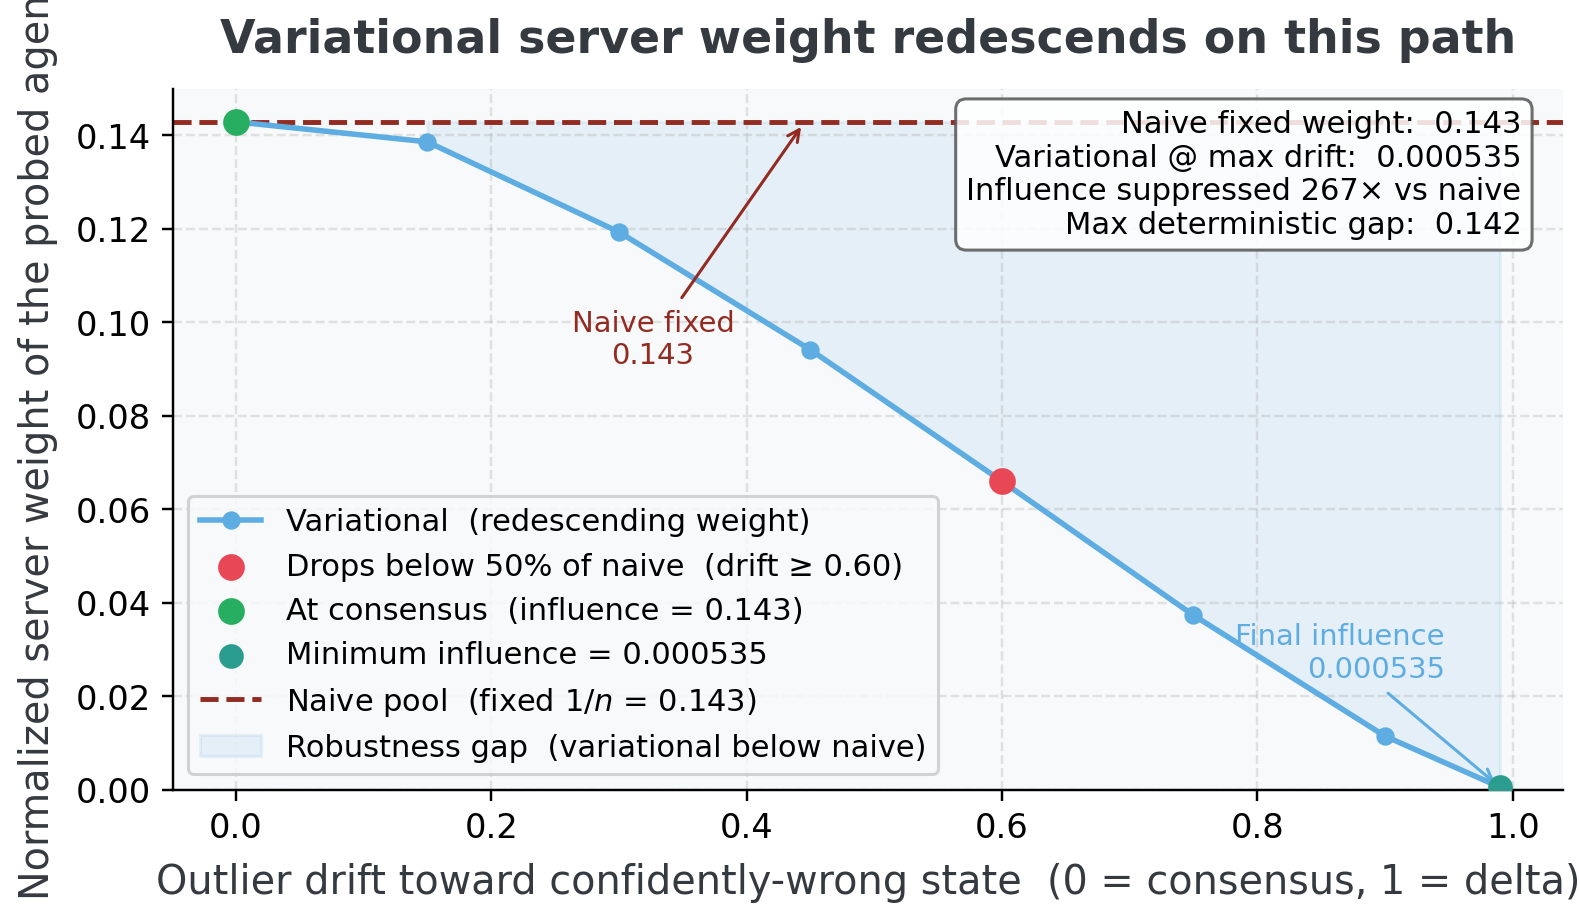
\includegraphics[width=0.8\linewidth,height=0.5\textheight,keepaspectratio,alt={An open-triangle dash-dot path shows a variational server's normalized influence weight falling as one agent drifts toward a confident-wrong belief. A circle-solid naive reference stays flat, direct endpoint labels identify both rules, and an X marks the first displayed half-weight crossing.}]{../figures/bounded_influence.png}
\caption{Normalized influence weight of one probed agent. Source
relation: original project variational-server diagnostic; estimand: the
probed agent's normalized server weight as its posterior drifts toward a
confident-wrong delta. The x-axis is outlier drift from consensus at
zero to the wrong-state delta at one; the y-axis is normalized influence
weight. The open-triangle dash-dot path is
\protect\breaktt{variational\_aggregate}; the circle-solid horizontal
reference is the naive log-linear pool. Direct endpoint labels name both
rules and values, shaded separation shows their tested-path gap, and an
adversarial X with an arrow marks the first displayed point below
one-half of the naive weight. As drift becomes extreme, the variational
weight falls below \(0.001\), whereas the naive pool remains fixed at
\(1/n=0.143\). This deterministic seeded sweep contains \(n=7\) agents
in one configured colony; drift points are ordered evaluations, not
independent replications, so no confidence interval or error band
applies. The pattern is redescending normalized weight along this path,
while the algebraic property bounds raw effective weight; the figure is
not an estimator-level B-robustness proof and does not transfer the
property to the sharper \protect\breaktt{robust\_aggregate}
heuristic.}\label{fig:bounded-influence}
\end{figure}

The honest trade is conservatism: because \(F\) carries the \(-H(q)\)
entropy term, its consensus is the maximum-entropy distribution
consistent with the weighted cross-entropies, deliberately flatter than
the product-of-experts. The variational aggregator therefore does
\emph{not} win the peak-accuracy verdict of
sec.~\ref{sec:results-verdict} --- that remains the sharp heuristic's
role --- and the two are reported as complements, never conflated:
rigor-with-conservatism on one side, accuracy-without-an-objective on
the other.

\subsection{Exploratory generalized-Bayes logistic-regression
baseline}\label{sec:results-baseline}

The sweep of sec.~\ref{sec:results-robustness} characterizes the
heuristic server axis. This exploratory baseline instead probes the
client-side axis in a synthetic point-estimate logistic-regression
setting. The cited robust-Bayes and federated- learning results provide
the source context
\citep{mcmahan2017communication, ashman2022partitioned, bui2018partitioned};
this finite experiment does not reproduce their source protocol or
inherit their conclusions unconditionally.

An exploratory federated logistic-regression point-estimate proxy is
trained under client label contamination. Standard clients use the NLL
gradient with L2 coefficient \(0.05\); the comparison uses the RCCE
gradient at \(q=1.00\) with L2 coefficient \(0.10\). The legacy
\breaktt{divergence="KLD"} and \texttt{divergence="AR"} arguments select
those coefficients for compatibility; this module does not evaluate KL
or Alpha-Rényi divergence between weight distributions, represent
posterior covariance, or implement a FedGVI generalized-posterior
objective. The estimand is therefore a composite contrast between two
joint loss-and-shrinkage configurations, not an isolated RCCE effect.
RCCE's \(q\to0\) gradient limit recovers the NLL gradient, while the
separate categorical recovery identities remain in
sec.~\ref{sec:results-recovery}.

The corresponding bounded-influence claim remains source-conditional on
FedGVI's assumptions \citep{mildner2025fedgvi}; this finite curve does
not test that theorem. The losses connect the density-power line
\citep{basu1998robust}, generalized cross-entropy
\citep{zhang2018generalized}, and the generalized-Bayes objective
\citep{bissiri2016general, knoblauch2022generalized}.

The displayed configuration uses \(q = 1.00\) and 200 points per class
per client. Those are configured inputs, not parameters selected by this
report. Only the peak-margin contamination level is selected within the
displayed contamination sweep, by the maximum composite-configuration
accuracy difference. The neighboring-\(q\) sensitivity check is
descriptive stability evidence, not leakage-free calibration or
confirmatory model selection.

As contamination rises, the two configuration curves remain close at
lower rates and separate over part of the moderate-to-high range. The
largest displayed composite-configuration mean difference occurs at 0.35
contamination, with margin 0.028. Neighboring tested loss parameters
retain a thresholded separation at more than one contamination level,
and the plotted bands are seed-level 95\% bootstrap intervals.

At the highest swept rate, 0.40, both configurations decline and no
reliable ordering remains. Retaining that endpoint is necessary for the
finite-sweep interpretation. Together with the within-sweep
peak-contamination selection, it makes this an exploratory conditional
pattern rather than a precalibrated or confirmatory robustness result.

The separation in this small logistic-regression setting is modest. The
recovery identities establish implementation compatibility at the named
limit (sec.~\ref{sec:results-recovery}); the bounded-influence result
comes from the cited FedGVI theorem under its assumptions
\citep{mildner2025fedgvi}, not from this curve's gap. Source-dataset
parity, leakage-free calibration, and posterior-uncertainty experiments
remain open (sec.~\ref{sec:future-scale}).

\begin{figure}
\centering
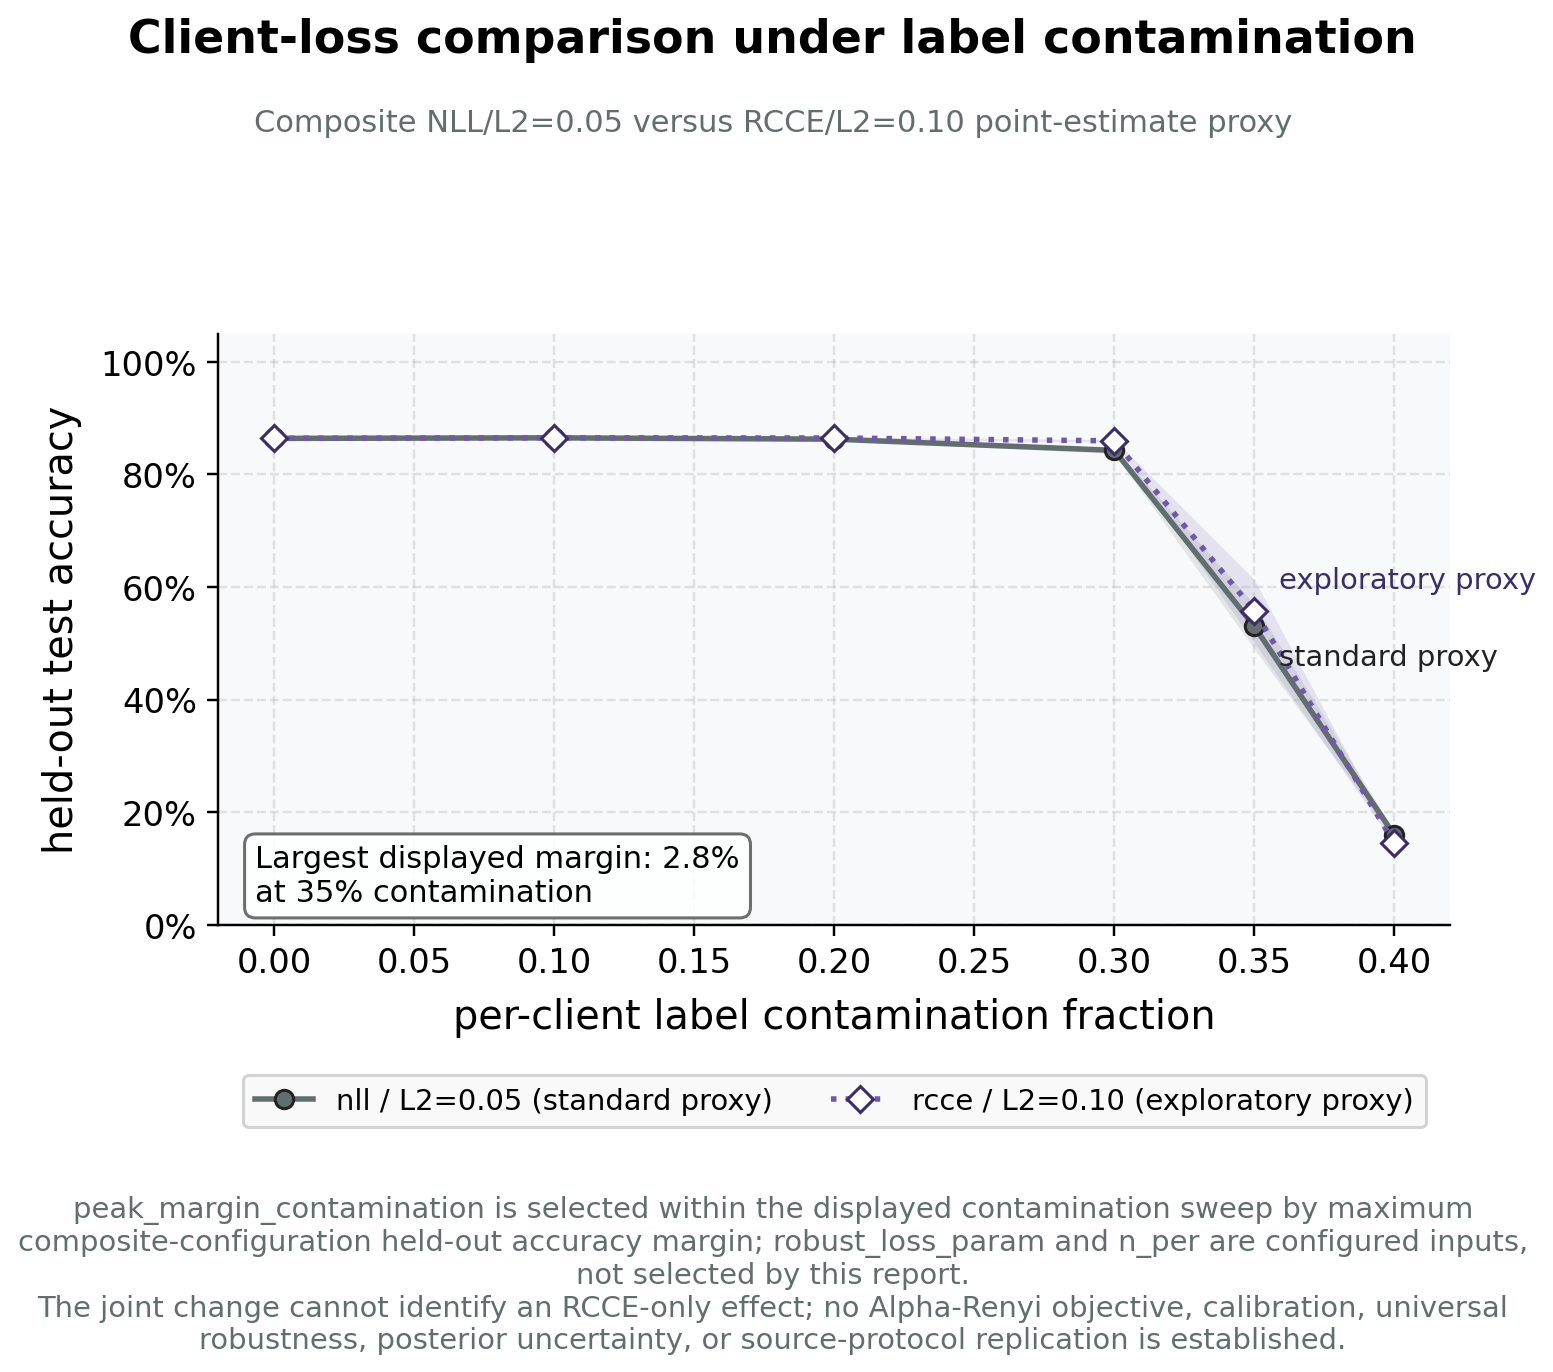
\includegraphics[width=0.8\linewidth,height=0.5\textheight,keepaspectratio,alt={Held-out accuracy curves compare joint NLL/L2=0.05 and RCCE/L2=0.10 configurations in an exploratory point-estimate logistic-regression proxy. Because loss and shrinkage change together, the contrast cannot isolate an RCCE-only effect. Seed intervals separate most at the within-grid selected peak contamination; both decline at the highest rate.}]{../figures/bnn_robustness.png}
\caption{Client-loss comparison under label contamination. Source
relation: exploratory original-project point-estimate
logistic-regression proxy; estimand: clean held-out accuracy for two
joint loss-and-L2 configurations; uncertainty: seed-level
percentile-bootstrap interval. The model uses one point-estimate weight
vector for each of 5 clients with 200 points per class per client; no
posterior covariance is computed. The x-axis is each client's
label-contamination fraction. The y-axis is held-out accuracy on a clean
synthetic test set, averaged over 64 independent seeds. Distinct markers
and line styles identify NLL with L2 coefficient \(0.05\) and RCCE with
L2 coefficient \(0.10\) at configured \(q=1.00\); bands show 95\%
seed-bootstrap intervals. Only the peak contamination is selected within
the displayed grid. Because loss and shrinkage change together, the
contrast cannot identify an RCCE-only effect. It does not establish
leakage-free calibration, universal robustness, posterior uncertainty,
an Alpha-Rényi result, or source-protocol
replication.}\label{fig:bnn-robustness}
\end{figure}

fig.~\ref{fig:bnn-robustness} is exploratory per-client proxy evidence.
Its loss-limit check, finite synthetic contrast, and the separate
source-conditional theorem have different roles; none comes from the
server comparison of sec.~\ref{sec:results-verdict}. The authoritative
three-axis boundary is sec.~\ref{sec:robustness-axes}.

\textbf{PyTorch deterministic-MLP complement (executed).} The optional
pipeline also instantiates generalized variational inference with a
point-mass MLP family: Linear\texorpdfstring{\ensuremath{\to}}{->}ReLU\texorpdfstring{\ensuremath{\to}}{->}Linear\texorpdfstring{\ensuremath{\to}}{->}softmax with 16 hidden units.
Clients use the density-power \(\beta\)-loss at \(\beta = 0.5\) for 200
Adam steps, and per-test-point predictions are fused with
\breaktt{robust\_aggregate} at \breaktt{robustness\ =\ 0.5} under PyTorch
2.12.1.

The executed consensus is a valid probability simplex, with maximum
unit-mass deviation 2.22e-16, and repeated seeded runs are bit-identical
(Yes). At contamination 0.40, held-out consensus accuracy is 0.558 for
the \(\beta\to 0\) client and 0.545 for the \(\beta=0.5\) client.

This single-seed endpoint demonstrates API transfer and deterministic
execution, not posterior-uncertainty inference, model-class
universality, or a robust-loss advantage at neural-network scale. It is
separate from the 64-seed exploratory logistic-regression curve above
and from the source-conditional theorem. When PyTorch is absent, the
pipeline records unavailable-value sentinels; builds exercising this
optional lane install the \texttt{torch} extra
(sec.~\ref{sec:reproducibility}).

\section{Discussion: what the evidence supports}\label{sec:discussion}

The 9 studies probe distinct parts of one categorical, factor-based
framework rather than repeating a single benchmark. Their common result
is narrow but useful: the client construction contains its
standard-Bayes limit and the server has a named project log-linear-pool
recovery corner, and behavior away from those limits can be measured
under declared contamination, sampling, and model assumptions. The
recovery identities are formal; the performance results are conditional
simulation evidence.

\subsection{The recovery limit is the formal
anchor}\label{sec:discussion-limit}

The coherence of the framework rests on the KL/NLL client limits and the
zero-robustness project-pool identity (eq.~\ref{eq:robust-identity},
eq.~\ref{eq:standard-bayes}). This is an identity of the stated
categorical implementation, not an asymptotic claim about every
generalized Bayesian model or a reconstruction of the complete source
protocol.

The server aggregator returns the log-linear pool
(eq.~\ref{eq:log-linear-pool}) with maximum deviation 0; the generalized
posterior returns the closed-form Bayes update with deviation 5.55e-17;
and the Rényi divergence, \(\beta\)-loss, and robust cross-entropy
recover their KL/NLL limits with residuals 0, 0, and 0.

Theorem \ref{thm:belief-sharing-recovery}, Corollary
\ref{cor:closed-form-bayes}, Lemma \ref{lem:renyi-kl-limit}, and
Proposition \ref{prop:robust-loss-recovery} state the formal limits; the
recovery checks in sec.~\ref{sec:results-recovery} are the executable
falsification harness.

\subsection{What the study suite jointly
shows}\label{sec:discussion-joint}

Read together, the suite separates into two kinds of result: identities
that hold exactly at the standard corner, and performance contrasts that
are explicitly conditional on the operating regime. The distinction is
the point of the joint reading --- it says which claims travel and which
are tied to the declared world.

Studies 1--3 sit at the standard corner. In the reduced categorical
analogue, the paired difference
\(\Delta \bar F=\bar F_{\text{solo}}-\bar F_{\text{share}}\) is 3.3109
nats, so its positive sign indicates lower mean free energy with
communication (sec.~\ref{sec:results-belief_sharing},
fig.~\ref{fig:free-energy}). Seeds are the independent unit; agents
remain nested within seed.

Dirichlet learning reduces KL from 3.4231 to 0.0027 nats
(sec.~\ref{sec:results-language}, fig.~\ref{fig:language-kl}). The
configured BMR sign control favors redundant-column pruning and rejects
the supported-column reduction (sec.~\ref{sec:results-emergence},
fig.~\ref{fig:emergence-bmr}). These are bounded mechanistic checks, not
exact source-protocol replications or general structure-discovery
results.

Study 4 steps away from the corner by holding the hidden state and
attack target fixed while redrawing matched contaminated colonies. The
standard pool degrades across the declared rate grid.

The server-side heuristic is not uniformly better: its robust members
are similar to or slightly below the standard pool at low contamination,
then the selected pooled display member separates in its favor under
severe contamination.

At the largest swept rate, AR reaches 0.9880 against 0.6928 for the
standard pool (tbl.~\ref{tbl:robustness_sweep}; the sweep plot in
fig.~\ref{fig:robustness-sweep} shows the separate matched-trial gallery
colony, whose largest-rate separation is smaller).

This regime dependence is a result, not a nuisance to be hidden:
robustness can cost efficiency when the attack is weak and pay off when
the declared contamination is severe.

The structural extension studies (Studies 5--9) sharpen the conditional
half of that split rather than adding further corner checks, and they
are reported with their negative contrasts intact. Communication is not
uniformly beneficial: the cross-study summary
(fig.~\ref{fig:cross-study-summary}) reports each study's federation
headline signed contrast or estimand in its native units. Its intervals
come from the separate harmonized seed-level rerun, including rows whose
primary figure is a deterministic diagnostic; several rows are positive,
while the moving-world EFE and two-level hierarchical rows are
approximately zero.

Pooling helps when views are complementary and can be unnecessary or
mildly costly when the agents already agree.

Adding hierarchical depth is held to the same standard --- the two-level
stack does not beat the flat baseline on location accuracy (the paired
gap is a small, statistically reliable cost)
(sec.~\ref{sec:results-hierarchical}), earning its place only by
additionally resolving the context latent above chance.

The joint lesson is therefore not that federation or depth is always
worth its cost, but that the suite measures the regimes in which each
one is.

\subsection{What this simulation identifies---and what it does
not}\label{sec:discussion-identifiability}

The primary robustness estimand is the matched-trial mean difference in
consensus accuracy conditional on the seeded true state and attack
geometry. The 960 paired trials quantify Monte Carlo variation for that
estimand; they do not average over hidden states, attack targets,
adaptive adversaries, or real deployments.

The cross-study layer reduces its matched trials within seed before
seed-level summaries, so clients and within-seed trials are not silently
counted as independent replicates.

This follows simulation study guidance to declare the estimand and Monte
Carlo unit explicitly \citep{morris2019simulation, koehler2009mcse}, and
the bootstrap interval follows the declared resampling unit rather than
treating nested observations as a flat sample
\citep{loy2021lmeresampler}.

The consequence is a more informative claim boundary. The sweep supports
a conditional statement about this contamination mechanism and these
categorical beliefs; it does not establish universal Byzantine
tolerance, calibration, or truth recovery.

The result also does not identify a single universally best robustness
parameter independent of the operating regime: the standard pool is
preferable at the low-contamination cells in this run, while at least
one robust member has a BH-rejected positive contrast in the declared
high-contamination verdict; the tied display set and deterministic
tie-break are reported separately.

Those are precisely the conditions a future adaptive or deployment study
must vary.

\subsection{The robustness comparison is conditional and statistically
qualified}\label{sec:discussion-verdict}

The headline comparison is computed by the statistics module
(sec.~\ref{sec:results-verdict}), not typed into the prose. Across 960
matched trial replicates nested within the fixed seeded world at
contamination rate 0.800, each robust server member is compared with the
standard pool by a Wilcoxon signed-rank test
\citep{wilcoxon1945individual} and the declared family of p-values is
adjusted by Benjamini--Hochberg FDR \citep{benjamini1995controlling}.

A method wins only when the adjusted null is rejected and its effect is
positive, here at \(q = 1.11 \times 10^{-158}\) with effect size 1.0000
(large). The observed-effect power and prospective sample-size
calculation are planning quantities, not independent confirmation of the
result.

The paired design is appropriate for the controlled comparison because
each condition shares the seed, true state, and attack geometry. Its
interpretation remains limited: the signed-rank test concerns the
distribution of paired differences, not equality of raw means, and BH
controls expected false-discovery proportion within the declared family
rather than the probability of any false positive.

The confidence intervals are percentile bootstrap intervals over the
matched-trial unit. Seed-level review-grid results are reported
separately and do not treat the primary trial count as a population of
independent worlds. These qualifications make the verdict narrower, but
also make it reproducible and falsifiable.

\subsection{Three robustness axes remain
separate}\label{sec:discussion-axes}

The authoritative theorem--heuristic--objective taxonomy is
sec.~\ref{sec:robustness-axes}. The results preserve it: the client
theorem remains source-conditional \citep{mildner2025fedgvi},
\breaktt{robust\_aggregate} carries only its proved recovery identity
plus conditional empirical contrasts, and
\breaktt{variational\_aggregate} carries the stated objective and
raw-weight bound. No figure or statistic moves a guarantee between these
operators; sec.~\ref{sec:limitations} records the complete boundary.

The map in fig.~\ref{fig:evidence-replication-map} is the compact ledger
for that separation. Its fourteen rows align headline result families
and public boundaries with their estimands and independent units, while
its nesting strip prevents seeds, trials, agents, and ordered states
from being treated as interchangeable evidence. Exact estimates and
intervals remain in their typed reports and the native-unit cross-study
summary (fig.~\ref{fig:cross-study-summary}).

\subsection{Accuracy and effective-weight control can be traded
explicitly}\label{sec:discussion-tempered}

The \(F_\lambda\) family (sec.~\ref{sec:supp-tempered}) supplies
empirical grid evidence that accuracy and effective-weight control need
not be a fixed binary choice within the tested objective family. At
\(\lambda = 1.0\) the implementation recovers the current variational
objective bit-for-bit; lower explored temperatures sharpen the consensus
toward the heuristic while preserving the stated raw-weight bound under
its assumptions.

This is not a derivation of the heuristic from an objective. The open
problem is to identify an objective whose minimizer is both competitive
across contamination regimes and accompanied by a theorem that survives
beyond the present categorical construction.

\subsection{Why the boundary matters
downstream}\label{sec:discussion-downstream}

The practical lesson is not that every robust rule should replace belief
sharing. It is that a multi-agent active-inference system can expose
separate controls for client updating, server reweighting, and
objective-backed consensus, while retaining a tested route back to the
ordinary pool.

That separation tells a builder what can be promised: exact recovery at
the named corner, conditional empirical behavior under the declared
attack, and no silent transfer of a client-side or variational theorem
to a different server heuristic. The result is a usable research
contract for extending belief-sharing systems without confusing a
simulation win with a general robustness guarantee.

\subsection{Related work: active inference, federated Bayes, and the
scoped bridge}\label{sec:related-work}

This work sits at the boundary between two research communities with
different objects of inference. Each cited thread contributes a real
component; this paper extends the intersection without claiming that
either literature is exhausted. The positioning is therefore against the
reviewed sources and their assumptions, not against an absolute claim
about everything the field has or has not done.

\subsection{Pre-modern probability, inverse probability, and collective
judgment}\label{sec:related-historical}

These historical sources provide conceptual lineage, not evidence that
early authors anticipated KL minimization, active inference, or
federation. Pascal and Fermat, Huygens, Montmort, Bernoulli, and de
Moivre made expectation and uncertain evidence objects of calculation
\citep{pascal1654probability, huygens1657ratiociniis, montmort1708essay, bernoulli1713ars, demoivre1718doctrine}.

Bayes and Price framed inference from observed events to an unknown
chance, and Laplace generalized inference about causes
\citep{bayes1763essay, laplace1774memoire}. Their relevance here is
vocabulary for generative-model inversion. The executable recovery
identity is instead a modern, project-local result of
sec.~\ref{sec:method-aggregation} and sec.~\ref{sec:formalism}.

Daniel Bernoulli's expected-utility treatment and the aggregation work
of Borda and Condorcet connect uncertain judgment to action and
collective choice
\citep{bernoulli1738mensura, borda1784elections, condorcet1785essai}.
They motivate questions about competence, independence, weights, and
stakes. They do not formally support this paper's log-pool,
generalized-Bayes, or robustness claims; the full genealogy remains
documented in the source audit.

\subsection{Active inference: generative agents, EFE, and
colonies}\label{sec:related-aif}

The free-energy principle \citep{friston2010free} and discrete
state-space process theory \citep{friston2017active} connect generative
models, variational inference, and expected-free-energy action
selection. The discrete synthesis \citep{dacosta2020active}, pymdp
\citep{heins2022pymdp}, and RxInfer \citep{bagaev2023rxinfer} provide
executable machinery. This project reimplements the categorical
substrate and its risk--ambiguity decomposition
(eq.~\ref{eq:efe-decomposition}, eq.~\ref{eq:efe-identity},
fig.~\ref{fig:efe-decomp}), then evaluates explicit robustness controls
at belief fusion.

The fusion operator itself is not new as a mathematical object. Under
the explicit categorical posterior-log-potential and fixed-weight bridge
of sec.~\ref{sec:method-aggregation}, the message-combination term of
Friston's belief-sharing equation is represented by a logarithmic
opinion pool \citep{genest1986combining, genest1986externally} and a
product-of-experts consensus \citep{hinton2002products}.

That limited representation is not a statement that the complete source
protocol is a log pool. Abbas' KL view of linear and log-linear pools
makes the same point in scoring-rule language: log-pooling can be
justified as a KL aggregation rule for expert distributions, not as a
contamination-robust estimator \citep{abbas2009kullback}.

The Bayesian Committee Machine adds the distributed-learning analogue:
independent estimators trained on data subsets can be combined by a
product-style Bayesian rule, with assumptions about conditional
independence and prior accounting made explicit
\citep{tresp2000bayesian}.

Fully Bayesian aggregation gives the social-choice counterpart:
geometric pooling of beliefs is singled out by dynamic Bayesian
rationality conditions, not by robustness to contaminated reports
\citep{dietrich2021fully}.

That classical literature is useful precisely because it names the
hidden commitments --- shared support, weight choice, prior accounting,
and external-Bayes coherence --- that are easy to overlook when the same
operation appears as a colony update.

A parallel thread studies how active-inference agents coordinate as
ensembles --- collective behavior and surprise minimization across a
colony \citep{heins2023collective}, epistemic communities
\citep{albarracin2022epistemic}, and collective intelligence
\citep{kaufmann2021collective}.

The belief-sharing thread \citep{friston2024federated} is one member of
this family. Agents fuse beliefs, and our colony scenario is a reduced
categorical standard- Bayes-limit analogue of its worked example
(eq.~\ref{eq:belief-round}, sec.~\ref{sec:results-belief_sharing}).

Structure learning completes the conceptual frame. Active inference with
Bayesian optimal design selects and reduces models
\citep{smith2020active}, while post-hoc BMR \citep{friston2011post}
motivates our configured sign control (eq.~\ref{eq:bmr-deltaf},
sec.~\ref{sec:results-emergence}).

Among the active-inference sources reviewed here, belief fusion is not
systematically characterized under explicit contamination or
intentionally wrong broadcasts, nor connected to the robustness theory
used here. Fusion is treated as trusting in that scoped comparison.

Friston et al. \citeyearpar{friston2024federated} present
communicating-colony free-energy convergence, Dirichlet language
acquisition, and Bayesian model reduction. We use reduced categorical
standard-Bayes-limit analogues of those mechanisms
(sec.~\ref{sec:results-recovery}) before the robust extension. The third
is a configured sign control on a fixed posterior. None is an exact
source-protocol or figure reproduction.

\subsection{Robust and federated Bayes outside active
inference}\label{sec:related-fl}

Federated learning aggregates models trained on decentralized data
\citep{mcmahan2017communication}, and the probabilistic-federation line
recasts that aggregation as variational inference --- partitioned
variational inference \citep{ashman2022partitioned} and its federated
predecessor \citep{bui2018partitioned}. This is a different use of the
word \emph{federated} from Friston et al.'s federated inference: Friston
federates hidden-state beliefs among agents sharing a world model, while
machine-learning federated learning usually federates parameter or
predictive-model updates over decentralized datasets.

The bridge claimed here is therefore algebraic and variational --- a
shared normalized product/log-pool operator at the KL/NLL recovery
corner --- not a claim that either source paper already solved the
other's problem.

Robustness, meanwhile, has a mature Bayesian theory: general Bayesian
updating through a loss \citep{bissiri2016general}, Gibbs posterior
inference \citep{jiang2008gibbs}, safe learning-rate selection under
misspecification \citep{grunwald2012safe}, coarsened posteriors for
robustness to exact-data conditioning \citep{miller2018coarsening},
divergence-criteria posterior updating \citep{jewson2018divergence},
Bayesian misspecification asymptotics
\citep{kleijn2012misspecification}.

The optimization-centric GVI view \citep{knoblauch2022generalized} and
recent closed-form characterizations \citep{nguyen2026closedformgvi}
connect objectives to approximating families. Bounded-influence
approaches include density-power and gamma-divergence estimation
\citep{basu1998robust, fujisawa2008robust, ghosh2015robust},
robust-divergence variational inference \citep{futami2018robustvi}, and
generalized cross-entropy \citep{zhang2018generalized}. Huber and
Ronchetti supply the robust-statistics vocabulary of influence and
breakdown \citep{huber2009robust}, used here for boundedness and
empirical failure modes rather than theorem transfer. FedGVI
\citep{mildner2025fedgvi} supplies the per-agent generalized-Bayes
synthesis with client and server divergence choices.

This literature provides decentralized aggregation and theorem-backed
results in its stated settings. Among the sources reviewed here, it does
not evaluate active-inference POMDP belief consensus---the
generative-model-bearing, action-selecting setting where beliefs drive
behavior.

The 2025 preprint on convergence rates under prior misspecification
\citep{mildner2025rates} sharpens the current GVI context: bounded
divergences can support concentration and rates under explicit
assumptions, but the result does not transfer automatically to this
repository's finite categorical state space or to its server-side
aggregation heuristic.

The federated-learning robustness literature also supplies important
negative space for this paper. Byzantine-tolerant gradient aggregation
\citep{blanchard2017krum}, geometric-median robust aggregation
\citep{pillutla2022robust}, and divergence-weighted gamma-mean
aggregation \citep{li2022gammafl} attack corrupted client updates
directly. A recent Bayesian robust-aggregation preprint likewise models
unknown client honesty for federated model updates
\citep{karakulev2025bayesian}.

Those are close comparators for adversarial federation, but the object
being aggregated differs: they aggregate model-update vectors or
posterior measures, while this paper attacks categorical belief fusion
and generalized-Bayes client updates.

Robust subset-posterior combination is another nearby Bayesian route
\citep{minsker2017median}, but it combines posterior measures across
data shards rather than active-inference belief broadcasts with a shared
latent state.

We use those sources to position the problem, not to import their
guarantees into \breaktt{robust\_aggregate}.

\subsection{The specific bridge added here}\label{sec:related-gap}

The scoped bridge evaluated by this manuscript is generalized-Bayes
belief fusion for active-inference ensembles. Concretely:

\textbf{Per-agent bounded-loss updates.} FedGVI-faithful \(\beta\)/rcce
updates carry the cited bounded-influence result only under its source
assumptions (eq.~\ref{eq:beta-loss}, eq.~\ref{eq:rcce-loss}).

\textbf{Server-side divergence reweighting.} The complementary heuristic
has a stated recovery limit (eq.~\ref{eq:robust-identity}). Its finite
empirical behavior does not borrow theorems from robust federated
aggregation.

\textbf{Recovery of the standard-Bayes corner.} The KL/NLL client limits
recover Bayes, while the separate zero-robustness server identity
returns the project log-linear pool (eq.~\ref{eq:standard-bayes},
eq.~\ref{eq:renyi-limit}, eq.~\ref{eq:robust-identity}). Under the
categorical bridge, that pool specializes only the Eq. 7
message-combination term \citep{friston2024federated}.

\textbf{Additional executed studies.} The source simulations motivate
mechanism analogues, not protocol recovery checks. Added studies cover
declared contamination (sec.~\ref{sec:results-robustness}), active
movement (sec.~\ref{sec:results-moving}), two- and three-level POMDPs
(sec.~\ref{sec:results-hierarchical}, sec.~\ref{sec:results-3level}),
finite acuity-by-colony sensitivity, and finite-grid acuity recovery
(sec.~\ref{sec:results-sensitivity},
sec.~\ref{sec:results-parameter-recovery}).

\textbf{Declared paired analysis.} The configured comparison uses
matched-pairs Wilcoxon tests
\citep{wilcoxon1945individual, fay2010wilcoxon}, Benjamini--Hochberg FDR
adjustment \citep{benjamini1995controlling}, percentile-bootstrap
intervals \citep{efron1993bootstrap}, rank/effect-size caveats
\citep{nakagawa2007effect}, and an observed-effect planning
approximation. These additions are project analyses, not claims about
the source paper.

\textbf{Objective-backed server control.}
\breaktt{variational\_aggregate} descends its stated free energy
(eq.~\ref{eq:agg-free-energy}); a converged fixed point is
coordinatewise stationary. The rule has a raw effective-weight bound and
a finite redescending diagnostic (fig.~\ref{fig:bounded-influence}).
Whether an equally defensible objective has the sharper reverse-KL
heuristic as its minimizer remains open.

The contribution is the bridge: an explicit connection between
active-inference belief consensus and robust federated generalized
Bayes, with the standard pool recovered exactly at the corner and the
additional studies (the contamination sweep plus several structural
extensions) showing how the bridge behaves beyond the Friston et
al.~baseline.

\subsection{Limitations and claim boundaries}\label{sec:limitations}

The boundaries here define the contribution. The central goal is to show
--- concretely and testably --- that the categorical
generalized-variational construction inspired by FedGVI
\citep{mildner2025fedgvi} has standard-Bayes client limits and a
project-local log-linear-pool server identity. Under the explicit bridge
in sec.~\ref{sec:method-aggregation}, the latter specializes Friston et
al.'s Eq. 7 message-combination term \citep{friston2024federated}, not
the complete source protocol; behavior away from those limits is
evaluated only under declared simulation conditions.

The exact identities are formal; performance and deployment claims
remain conditional. Items beyond that boundary are named as future work.

\subsection{Three robustness axes: theorem, heuristic, and
objective}\label{sec:limitations-axes}

The authoritative definitions and claim owners are in
sec.~\ref{sec:robustness-axes}; this section records only what still
cannot transfer. A source-conditional client theorem does not certify
either server rule, a server recovery identity does not supply an
objective or estimator-level influence bound, and objective descent plus
raw-weight control does not imply truth recovery or peak-accuracy
dominance. Likewise, conditional accuracy contrasts cannot confer a
theorem on the heuristic. The evidence map in
fig.~\ref{fig:evidence-replication-map} makes that no-transfer boundary
and its nested replication units explicit.

The remaining methodological problem is a server objective that combines
competitive conditional performance with an appropriate robustness
guarantee. Related robust-federation work motivates the target
\citep{blanchard2017krum, li2022gammafl} but does not certify either
project server rule. Any such result must also survive beyond the
present categorical model, declared attack grid, and single-host
execution setting; future work and extended methods remain separate
(sec.~\ref{sec:future}, sec.~\ref{sec:supp-extended}).

\subsection{Scope boundaries that the evidence does not
cross}\label{sec:limitations-scope}

\textbf{The bridge is a recasting, not an upstream claim.} Friston et
al. \citep{friston2024federated} supply a belief-sharing operator for
agents with a shared world model; Mildner et al.
\citep{mildner2025fedgvi} supply robust federated generalized
variational inference. Neither paper claims the other. The contribution
here is to recast the former as the tested KL/NLL zero-robustness
recovery corner of the latter-inspired construction, then measure
changes under robust losses and server reweighting.

\textbf{Historical sources are conceptual, not formal support.} The
pre-modern sources added in sec.~\ref{sec:related-historical} support a
genealogy of expectation, inverse inference, utility, and collective
judgment
\citep{huygens1657ratiociniis, bayes1763essay, laplace1774memoire, bernoulli1738mensura, condorcet1785essai}.
They do not support claims about KL, NLL, product-of-experts training,
FedGVI, or \breaktt{robust\_aggregate}.

Those claims rest only on the modern cited formalism and the tests
reported in sec.~\ref{sec:results-recovery}.

\textbf{Single-machine federation.} Federation is validated with queue
transport, a single-machine OS-process helper, and loopback TCP: agents
serialize beliefs, the server aggregates, and consensus is broadcast
back without changing the mathematics. The socket path exercises frame
integrity and file-backed digest-verified replay validation; an optional
SQLite round-ID guard survives local process restarts.

These controls do not substitute for cross-host deployment,
identity-bound mTLS, a shared multi-host replay domain, discovery,
long-running worker orchestration, or fault tolerance; those steps are
scoped as future work (sec.~\ref{sec:future}).

\textbf{Source-scale posterior FedGVI classification remains open.} The
displayed NumPy logistic-regression baseline is an exploratory
point-estimate comparison, not the source paper's posterior-uncertainty
BNN experiment \citep{mildner2025fedgvi}. Its operating point was
selected within the evaluated synthetic sweep to expose a
mid-contamination margin (fig.~\ref{fig:bnn-robustness}).

The curves lose reliable ordering at the highest rate. The source
theorem, not this selected finite sweep, carries the source-conditional
robustness claim.

\textbf{Classification baselines are point estimates, not full
posteriors.} The NumPy logistic-regression baseline and the PyTorch MLP
complement both use point-estimate weights; no posterior covariance is
computed.

A genuine mean-field variational family over the
weights---diagonal-Gaussian \(q(w)\) with a closed-form KL and a
Monte-Carlo ELBO---is implemented by the tested \texttt{VariationalMLP}
primitive in the \breaktt{bnn\_variational\_torch} module. It recovers
the point-estimate net exactly as its posterior variance vanishes.

The source-comparable training and evaluation lane remains unexecuted:
leakage-free calibration, source-dataset parity, posterior-family
comparisons, and source-scale compute are still open.

\textbf{Hierarchical depth does not by itself improve the base task.}
The two- and three-level stacks (sec.~\ref{sec:results-hierarchical},
sec.~\ref{sec:results-3level}) run alternating L1/L2(/L3) inference
end-to-end and resolve their added context latents above chance. On the
shared location task they do not beat the flat baseline: the paired
location-accuracy gap is a small, statistically reliable negative gap at
the reported seed count (fig.~\ref{fig:hierarchical-pomdp}).

Depth is therefore validated as executable and consensus-preserving, not
as an accuracy improvement; whether a richer policy-and-horizon task
family rewards hierarchy is future work
(sec.~\ref{sec:future-hierarchical}).

\textbf{Discrete POMDP only---continuous or hybrid state spaces are not
addressed.} This work is discrete-categorical only, matching the
community's worked POMDP example
\citep{dacosta2020active, friston2024federated}. The limit-as-proof
contract is validated off the categorical case only for a
one-dimensional Gaussian-mean conjugate slice; continuous-state active
inference and Gaussian belief-sharing colonies remain untested.

\textbf{Temperature and divergence calibration are fixed, not learned.}
Coarsened posterior and safe-Bayes theory make clear that the
learning-rate/temperature is part of the inference rule under
misspecification
\citep{miller2018coarsening, grunwald2012safe, kleijn2012misspecification}.
This manuscript validates the configured losses and divergences, but it
does not learn an optimal coarsening radius, temperature, or divergence
schedule across agents.

\textbf{Real multi-machine federation, networking, and privacy
cryptography.} Federation here is \emph{mathematical} (factor
aggregation), not infrastructural--- unlike communication-efficient or
Byzantine-robust federated learning
\citep{mcmahan2017communication, blanchard2017krum}.

\textbf{New linguistic theory.} The language-acquisition study
(sec.~\ref{sec:results-language}) reproduces the Dirichlet count
mechanism (eq.~\ref{eq:dirichlet-update}) mechanically; it does not
extend the linguistics.

\subsection{What the statistics can and cannot
claim}\label{sec:limitations-stats}

The verdict is a paired comparison at a single high contamination rate
(sec.~\ref{sec:results-verdict}, tbl.~\ref{tbl:robustness_verdict}). The
design concentrates power where the effect is largest. It therefore
identifies \emph{where} robustness pays off, but it does not
characterize contamination as a continuous function. The per-rate effect
and inference projections
(tbls.~\ref{tbl:paired-by-rate}, \ref{tbl:paired-by-rate-inference})
describe the remaining sweep. Their inferential claims do not exceed the
declared BH-FDR control \citep{benjamini1995controlling}.

BH-FDR controls expected false discovery proportion within the declared
family, not the chance of any false positive. The matched-pairs Wilcoxon
tests are rank tests under paired-difference assumptions
\citep{wilcoxon1945individual, fay2010wilcoxon}, not assumption-free
proofs about raw means.

Confidence intervals are percentile bootstrap
\citep{efron1993bootstrap}, not analytic, and inherit that method's
small-sample caveats at the lowest trial counts.

The power values are observed-effect design approximations useful for
confirmatory sample-size planning; they are not independent evidence for
the verdict and do not cover model-specification uncertainty outside the
seeded simulation harness \citep{wasserstein2016asa}.

\subsection{Future work: testing the open boundaries}\label{sec:future}

The staged research program follows directly from the boundaries in
sec.~\ref{sec:limitations}. It separates public-library reproducibility,
server theory, portable source-protocol work, task generalization, and
deployment validation so that success in one lane cannot silently
certify another.

The order is deliberate. Simulation-study guidance recommends declaring
the estimand, data-generating mechanism, and Monte Carlo precision
before treating replication as evidence \citep{morris2019simulation},
while Monte Carlo error should be reported separately from an interval
or a hypothesis test \citep{koehler2009mcse}.

For nested agents, trials, and seeds, the resampling unit must respect
the dependence structure \citep{loy2021lmeresampler}. Accordingly, the
phase plan records a primary unit and a falsifier for each extension; a
larger sample or more elaborate diagram is not itself a stronger claim.

The implementation registry also separates smoke, pilot, and
confirmatory profiles. Pilot worlds select budgets and calibration
settings but never enter confirmatory intervals or headline values.

Each completed run must bind its source bundle, configuration, dataset
bytes, device, checkpoints, outputs, and completion status into a
verifiable receipt. A negative or null scientific result remains a valid
citable outcome when those implementation and provenance gates pass; it
blocks the intended positive claim, not the software release.

A separate Friston protocol lane will resolve a machine-readable parity
matrix before reconstructing source experiments in Python. Until every
required source parameter, routine, unit, and estimand is recovered,
that lane will be described as a paper-constrained reconstruction rather
than an exact replication.

\subsection{Make the sharp server heuristic
variational}\label{sec:future-server}

The asymmetry between the robustness axes
(sec.~\ref{sec:robustness-axes}) motivates a consequential theoretical
design question that is explicitly parked outside the authorized
roadmap. The client-side \(\beta\)/rcce update carries a derived,
loss-specific bounded-influence result under the matching assumptions;
the sharp server-side \breaktt{robust\_aggregate} carries only its
recovery limit (eq.~\ref{eq:robust-identity}).

The new variational aggregator (sec.~\ref{sec:method-variational},
sec.~\ref{sec:supp-variational}) supplies a \emph{rigorous} server-side
rule --- exact block updates descending the stated free energy
eq.~\ref{eq:agg-free-energy} through non-increasing block updates, with
a proven raw effective-weight bound and the same recovery corner. What
it costs is conservatism: it is the maximum-entropy consensus, not the
sharp accuracy-maximizer.

That parked question is sharper than before: write down a generalized
variational objective in the FedGVI family \citep{mildner2025fedgvi},
informed by recent closed-form GVI characterizations
\citep{nguyen2026closedformgvi}, logarithmic-pool weighting theory
\citep{carvalho2023logpooling}, and robust divergence-weighted federated
aggregation \citep{li2022gammafl}, whose closed-form minimizer is
competitive with the empirical reweighting across declared contamination
regimes.

That would combine axis 3's effective-weight bound with axis 2's
empirical sharpness in one server rule. The recovery corner and the
variational objective together supply two boundary conditions any such
unification must satisfy.

Any empirical choice of \texttt{robustness} or \texttt{entropy\_weight}
will be made on separate calibration worlds using a proper log score,
then frozen before confirmatory evaluation. This guards against
selecting an apparent leader with evaluation truth and preserves null or
reversed confirmatory outcomes.

The comparison family will include logarithmic and linear pools, the
current heuristic, the variational family, and a centered-log-ratio
geometric-median control; none inherits a parameter-space
robust-federated-learning guarantee merely by operating on beliefs.

\subsection{Promote the baseline to original FedGVI
scale}\label{sec:future-scale}

The bounded-influence result is anchored locally by the small NumPy
logistic-regression baseline (fig.~\ref{fig:bnn-robustness}). Promoting
it to the GPU-scale Bayesian-neural-network experiments of the source
paper \citep{mildner2025fedgvi} --- the experiments deferred here
(sec.~\ref{sec:limitations}) --- would test whether the per-client
robustness curve holds at the model capacity and contamination regimes
where federated learning \citep{mcmahan2017communication} actually
operates.

It would connect the discrete-POMDP result to the partitioned-VI line
\citep{ashman2022partitioned, bui2018partitioned}. The planned
comparison would also require posterior-parameterization parity with
Bayesian neural-network work, rather than treating the current
deterministic point-mass MLP as a posterior \citep{mildner2025fedgvi}.

The portable lane preserves the source protocol's site factors, client
cavity, factor-replacement update in natural coordinates. A synthetic
CPU/MPS pilot already exercises the cavity-conditioned local optimizer,
explicit device and fallback receipts, and checkpoint/resume
equivalence. It does not establish source-dataset parity.

The next local campaign distinguishes a locked portable CPU/MPS profile
from an exact source-scale CUDA profile that remains external until
suitable hardware is available. FashionMNIST anchors source-dataset
protocol parity, while MNIST and KMNIST test portability.

A separate source-bound tabular pack will report proper-score effects
per licensed dataset, with training-only preprocessing and byte-,
split-, and license-level provenance; nested seeds will not be treated
as independent datasets.

\subsection{Extend hierarchical federation beyond the current
stack}\label{sec:future-hierarchical}

The governing caveat here is that added depth must be shown to
\emph{earn} generalization, not merely to execute: on the current
sentinel task the deeper stacks match rather than beat the flat baseline
on location (sec.~\ref{sec:limitations-scope}). The extension therefore
has two distinct fronts --- carrying the recovery contract to deeper
stacks, and finding a task family in which depth actually pays.

The 2-level hierarchical POMDP (sec.~\ref{sec:results-hierarchical})
couples location inference to a single global context. The generic
N-level architecture uses \breaktt{build\_nlevel\_world} from the
\breaktt{fedference.pomdp} module and has already been exercised with a
3-level stack (sec.~\ref{sec:results-3level},
sec.~\ref{sec:supp-3level}): a meta-context variable (L3) gates the
context prior (L2) which in turn gates the location prior (L1).

The empirical-prior top-down messages (eq.~\ref{eq:l3-to-l2-message},
eq.~\ref{eq:l2-to-l1-message}) remain valid variational steps at every
depth, and the log-linear-pool federation at each level is bit-identical
to the in-process result (Proposition
\ref{prop:federation-bit-identity}).

The natural next question is whether the limit-as-proof contract of
sec.~\ref{sec:limitations} survives still deeper hierarchies: does the
recovery corner (context prior \texorpdfstring{\ensuremath{\to}}{->} uniform) remain checkable to machine
precision when the L2 \texorpdfstring{\ensuremath{\to}}{->} L1 message is itself a function of an L3 belief
coupled to an L4 belief, and can message-passing engines such as RxInfer
\citep{bagaev2023rxinfer} carry the generic alternating-minimization at
scale?

The current hierarchical diagnostic asks a narrower question. Under one
configured surprise threshold, it classifies the non-gating top level
below the threshold and the informative top level above it
(sec.~\ref{sec:results-hierarchical-bmr}). This is an implementation
control, not a posterior refit or an autonomous depth-selection result.

A future breadth-and- depth search must define its candidate family,
scoring rule, uncertainty, replication units, and out-of-sample
evaluation before it can support a model- selection claim for the
generic N-level stack.

The next task family is deliberately controlled rather than merely
deeper: partially observable Four Rooms and Key-Door will compare flat,
oracle, learned, shuffled, and non-gating hierarchies at matched
horizons and compute. Task is the higher-level replication unit. A gain
in only one task will remain task-specific, and the larger campaign will
not begin until the hybrid representation recovery gates pass.

\subsection{Move from process transport to true multi-machine
federation}\label{sec:future-transport}

The current deployment uses queue-backed single-machine processes and
loopback sockets. Promotion to cross-host workers would address the
remaining deployment caveat of sec.~\ref{sec:limitations}. That
extension must preserve the bit-identical consensus property proved in
Proposition \ref{prop:federation-bit-identity}.

The \texttt{federation/} package and federation tests already establish
the API contract: a server collects serialized beliefs from 5 worker
channels, fuses them with \breaktt{robust\_aggregate} at robustness
\(c = 1.5\), and broadcasts the consensus back over response channels,
with bit-identity verified at True.

The loopback socket path adds optional pre-shared-key frame integrity
and file-backed digest-verified replay validation. The next systems step
is an explicitly local Docker multi-node emulator with mTLS by default,
HMAC compatibility, checkpoint/restart, and reproducible message-fault
controls. It is not physical multi-host evidence.

That later claim requires receipts from distinct hosts, deployment-grade
key management, timeout policy, and long-running orchestration across
process restarts, but it does not require changing the mathematics.

Secure aggregation, differential privacy, and Byzantine tolerance are
separate future threat models; transport integrity alone would not
establish any of them \citep{blanchard2017krum, pillutla2022robust}.

\subsection{Move beyond categorical state
spaces}\label{sec:future-continuous}

This work is discrete-categorical, matching the community's worked POMDP
\citep{dacosta2020active}. A first step is already in place: the
closed-form Gaussian KL and Rényi divergences of
sec.~\ref{sec:supp-extended} show the divergence family --- and its
\(\alpha\to1\) recovery --- carries over verbatim to Gaussian beliefs,
scoped out of the categorical experiments.

Continuous-state Gaussian generative models would test whether the
limit-as-proof contract survives the move off categorical state spaces
--- whether the recovery corner remains checkable to machine precision
when the belief simplex is replaced by a Gaussian belief, and whether
message-passing engines such as RxInfer \citep{bagaev2023rxinfer} can
carry the robust update at scale.

Extending the structure-learning study
\citep{smith2020active, friston2011post} into continuous models would,
in parallel, test whether robust belief fusion and robust
\emph{structure} fusion compose.

A minimal executable fixture now gates a discrete dynamics context over
continuous position and velocity, Gaussian observations, and bounded
actions. The bounded pilot now includes matched naive, robust,
discrete-only, continuous-only, and oracle-context components, a
singular-covariance rejection, and next-position predictive scoring.

It is still a representation, recovery, and control surface rather than
confirmatory task evidence. The full study must freeze calibration and
budgets, use independently held-out worlds, retain outlier falsifiers,
and execute the preregistered comparison before supporting a hybrid-task
claim.

\section{Conclusion: a recovery-tested bridge with bounded
claims}\label{sec:conclusion}

Active Fedference makes a deliberately narrow bridge between two bodies
of work that are usually discussed with different objects and different
standards of evidence. Active inference describes agents that infer and
act within generative models; federated generalized Bayes describes how
losses, divergences, and variational objectives can make decentralized
inference less sensitive to bad information
\citep{friston2017active, dacosta2020active, bissiri2016general, knoblauch2022generalized}.

This paper does not dissolve those distinctions. It puts them into one
categorical implementation, identifies the exact point at which they
coincide, and then measures the consequences of moving away from that
point.

\subsection{The durable result is a recovery
contract}\label{sec:conclusion-recovery}

The central contribution is the recovery-tested contract. The KL/NLL
client limits of the declared generalized-Bayes construction recover the
closed-form Bayes update, while the zero-robustness server branch
recovers the project log-linear pool, with maximum measured deviations
of 5.55e-17 and 0 (eq.~\ref{eq:standard-bayes};
eq.~\ref{eq:robust-identity}).

This is stronger than a verbal analogy because the limited identities
are stated in the formalism, implemented in the core, and checked by
executable invariants.

Under the explicit shared-support, posterior-log-potential, and
fixed-weight bridge, the server pool specializes Eq. 7's
message-combination term; it is not an assertion that the
active-inference and robust-Bayes literatures share all assumptions,
objectives, deployment meanings, or the complete source protocol.

That distinction matters historically and methodologically. Logarithmic
pooling has a substantial literature as an aggregation rule for expert
distributions, including its connections to external Bayesianity,
product-of-experts constructions, and KL-based opinion pooling
\citep{genest1986combining, genest1986externally, hinton2002products, abbas2009kullback, dietrich2021fully}.

FedGVI contributes a generalized-Bayes perspective in which the loss and
divergence determine what robustness means \citep{mildner2025fedgvi}.

The contribution here is therefore a scoped recasting: the project's
categorical log-linear-pool specialization is the non-robust corner of
the implemented family under its stated bridge assumptions, and the
corner becomes a testable boundary condition for future robust
extensions.

This does not identify the complete source belief-sharing protocol with
FedGVI.

\subsection{What the evidence establishes away from the
corner}\label{sec:conclusion-evidence}

The standard-Bayes studies provide a necessary baseline rather than
ornamental background. Communication changes mean free energy by 3.3109
nats, Dirichlet learning reduces KL from 3.4231 to 0.0027, and the
configured BMR sign control favors the declared redundant pruning while
rejecting the supported control. These bounded diagnostics retain the
stated categorical source relation \citep{friston2024federated}; they do
not establish universal structure discovery or exact source-protocol
replication.

The extension studies show that communication is not automatically
beneficial in every information geometry. Disjoint views can make
sharing valuable, whereas a complementary moving-world control can make
additional pooling unnecessary or mildly costly.

The contamination study adds a second lesson. The server-side heuristic
is regime-dependent: robust operating points can give up a little
efficiency when contamination is weak and recover that cost when the
declared attack is severe.

At the most severe swept rate, the highest robust consensus mass in the
single-world mechanistic sweep reaches 0.9880 (AR) against the standard
pool's 0.6928 (tbl.~\ref{tbl:robustness_sweep}); at the verdict rate,
the matched, BH-adjusted comparison for RKL in
sec.~\ref{sec:results-robustness} gives 0.9829 against 0.9021.

The result is therefore an operating-point contrast, not a ranking that
holds for every contamination rate, attack target, hidden state, or
calibration regime.

This interpretation follows the simulation-study principle that the
data-generating mechanism, estimand, and Monte Carlo unit should be
declared before a numerical result is treated as general evidence
\citep{morris2019simulation}.

The authoritative three-axis map is sec.~\ref{sec:robustness-axes}. The
client theorem remains source-conditional, the
\breaktt{robust\_aggregate} results remain heuristic and conditional, and
\breaktt{variational\_aggregate} retains its stated objective and raw-
weight bound. Keeping those claim owners separate prevents a guarantee
proved for one operator from migrating to another merely because both
are called ``robust.''

\subsection{Why the bridge matters for active
inference}\label{sec:conclusion-significance}

Belief sharing is not merely a communication convenience. In an
active-inference system, a shared posterior can change expected
free-energy calculations, model comparison, and subsequent action
selection. A robustification at the fusion step can therefore alter
behavior even when each local generative model is unchanged.

Conversely, a server rule that suppresses an anomalous belief may also
suppress a rare but correct observation. The relevant scientific
question is not simply whether a robust curve rises; it is which
assumptions about competence, independence, support, and action-relevant
uncertainty the fusion rule encodes
\citep{genest1986combining, tresp2000bayesian, heins2023collective}.

This is why the recovery corner is a useful organizing device. It gives
a common reference behavior before robustness is introduced, makes the
cost of a server intervention measurable, and lets later work compare
new aggregation rules against an interpretable baseline.

The bridge also keeps the distinction between inference and
infrastructure visible. The current federation tests show that
serialized beliefs can travel through the declared local transport and
return a bit-identical consensus, but they do not turn a mathematical
aggregation identity into a claim about secure, fault-tolerant, or
privacy- preserving deployment
\citep{mcmahan2017communication, blanchard2017krum, pillutla2022robust}.

\subsection{What remains unproved}\label{sec:conclusion-boundaries}

The evidence does not establish universal Byzantine tolerance, truth
recovery, calibration, or an optimal robustness parameter.

The primary intervals are conditional on the fixed hidden state and
attack target, and the nested trial and seed structure is reduced at the
declared unit rather than treated as a larger independent sample
\citep{koehler2009mcse, loy2021lmeresampler}. The categorical state
space is the object of the proof and experiment; continuous or hybrid
state spaces are a separate mathematical extension.

The neural classification complement uses point-estimate weights, so it
does not establish full posterior FedGVI behavior at the scale of the
source experiments.

These are not defects to be hidden by a more expansive title. They
define the proper contribution: an executable categorical bridge, a
recovery certificate, an explicit map of theorem-bearing and heuristic
components, and conditional evidence about contamination behavior.
Robust-statistics language such as influence and breakdown remains
useful for describing the failure modes, but a finite simulation sweep
is not by itself a general estimator-level robustness theorem
\citep{huber2009robust}.

The same discipline applies to historical and conceptual scholarship:
early work on probability, inverse inference, utility, and collective
judgment supplies lineage, not evidence for modern KL, FedGVI, or
adversarial-federation claims.

\subsection{A falsifiable research
program}\label{sec:conclusion-program}

The next stage should be organized around boundary conditions rather
than a larger collection of demonstrations. First, derive a server
objective whose minimizer is competitive with \breaktt{robust\_aggregate}
while retaining the variational rule's effective-weight control. Recent
work on closed-form generalized variational objectives, logarithmic-pool
weighting, and robust divergence-weighted federation provides relevant
mathematical constraints
\citep{nguyen2026closedformgvi, carvalho2023logpooling, li2022gammafl}.

A useful candidate must recover the standard log-linear pool at zero
robustness, state which quantity is bounded, and fail visibly when those
assumptions are violated.

Second, broaden the primary estimand across attack targets, hidden
states, adaptive adversaries, calibration conditions, and model classes.
The decisive falsifier is not a lower average score on one new grid; it
is failure of the claimed robustness advantage, recovery identity, or
stated uncertainty calibration under a pre-registered extension of the
data-generating mechanism.

Third, promote the point-estimate neural complement to a
posterior-parameterized FedGVI study at source-comparable scale, and
test whether the client-side bounded-loss behavior survives capacity,
optimization, and posterior-family changes.

Finally, move from local transport to multi-machine execution with
explicit threat models, authentication, failure handling, and privacy
claims; none should be inferred from the current bit-identity result.

\subsection{Final position}\label{sec:conclusion-position}

The strongest conclusion is consequently neither that robust belief
sharing has been solved nor that the bridge is merely metaphorical. In
the declared categorical setting, the standard-Bayes client limits and
project log-linear-pool server identity are tested recovery conditions;
away from them, server behavior is measurable, regime-dependent, and
partitioned into theorem-bearing, objective-backed, and heuristic
claims.

That is a modest result, but it is a useful one: it supplies a
reproducible starting point from which stronger theorems, broader state
spaces, independent implementations, and real federated deployments can
be judged without losing the baseline they are meant to extend.

\section{Reproducibility: execution record and application
integrity}\label{sec:reproducibility}

This section is a machine-verifiable reproducibility certificate. Every
value below is computed by the analysis pipeline and injected at render
time, establishing a chain of custody from configuration through code to
publication.

The discipline is the one that gates this project's CI: every prose
number is a generated token, every token is emitted by one generator
function, and any drift between narrative and computed result fails the
build before a green PDF exists \citep{peng2011reproducible}.

\subsection{Determinism contract for seeded scientific
results}\label{sec:repro-determinism}

Reproducing every reported number requires only two recorded inputs: the
global seed pinned here and the software environment fingerprinted in
the next subsection. The determinism contract fixes the first --- it
states exactly what is held constant, what is asserted to machine
tolerance, and what is deliberately not claimed byte-identical.

\textbf{Seed.} The global seed is 0, threaded through every
\breaktt{np.random.default\_rng(seed)}; the global \texttt{np.random}
state is never used.

\textbf{Assertions.} Recovery identities use exact or machine-tolerance
assertions; seeded study reports are regression-tested for repeatability
under the recorded software environment. Rendered PDF/HTML/slide
containers are validated as fresh publication products but are not
claimed byte-identical across toolchain versions.

\textbf{Execution.} No mocks are used: every test is a genuine
computation on small categorical distributions or a seeded simulation
under this repository's explicit no-mocks policy.

\subsection{Application integrity and solver-health
receipts}\label{sec:repro-application-integrity}

The labeled own-data path produces a different evidentiary object from a
research report. It validates one-dimensional categorical inputs, hashes
the canonical semantic request, delegates once to the shared aggregation
domain, and records numerical health without adding a decision or
interpretation.

The application flow in fig.~\ref{fig:application-integrity-flow} reads
from top to bottom. Panel A follows validation and canonical hashing;
Panel B places the exact two-by-two \texttt{solver\_status} key below
the result classifier; Panel C separates the upper atomic-write row from
the lower verification lane. Invalid inputs or unsafe destinations fail
before directory creation. Non-nominal numerical results retain their
artifacts and return a distinct status rather than being silently
promoted or discarded.

An application receipt can verify artifact integrity and, when requested
and available, source equivalence. Requiring nominal solver health adds
a numerical gate. None of those levels establishes calibration, domain
suitability, scientific validity, decision correctness, or acceptance.

\begin{figure}
\centering
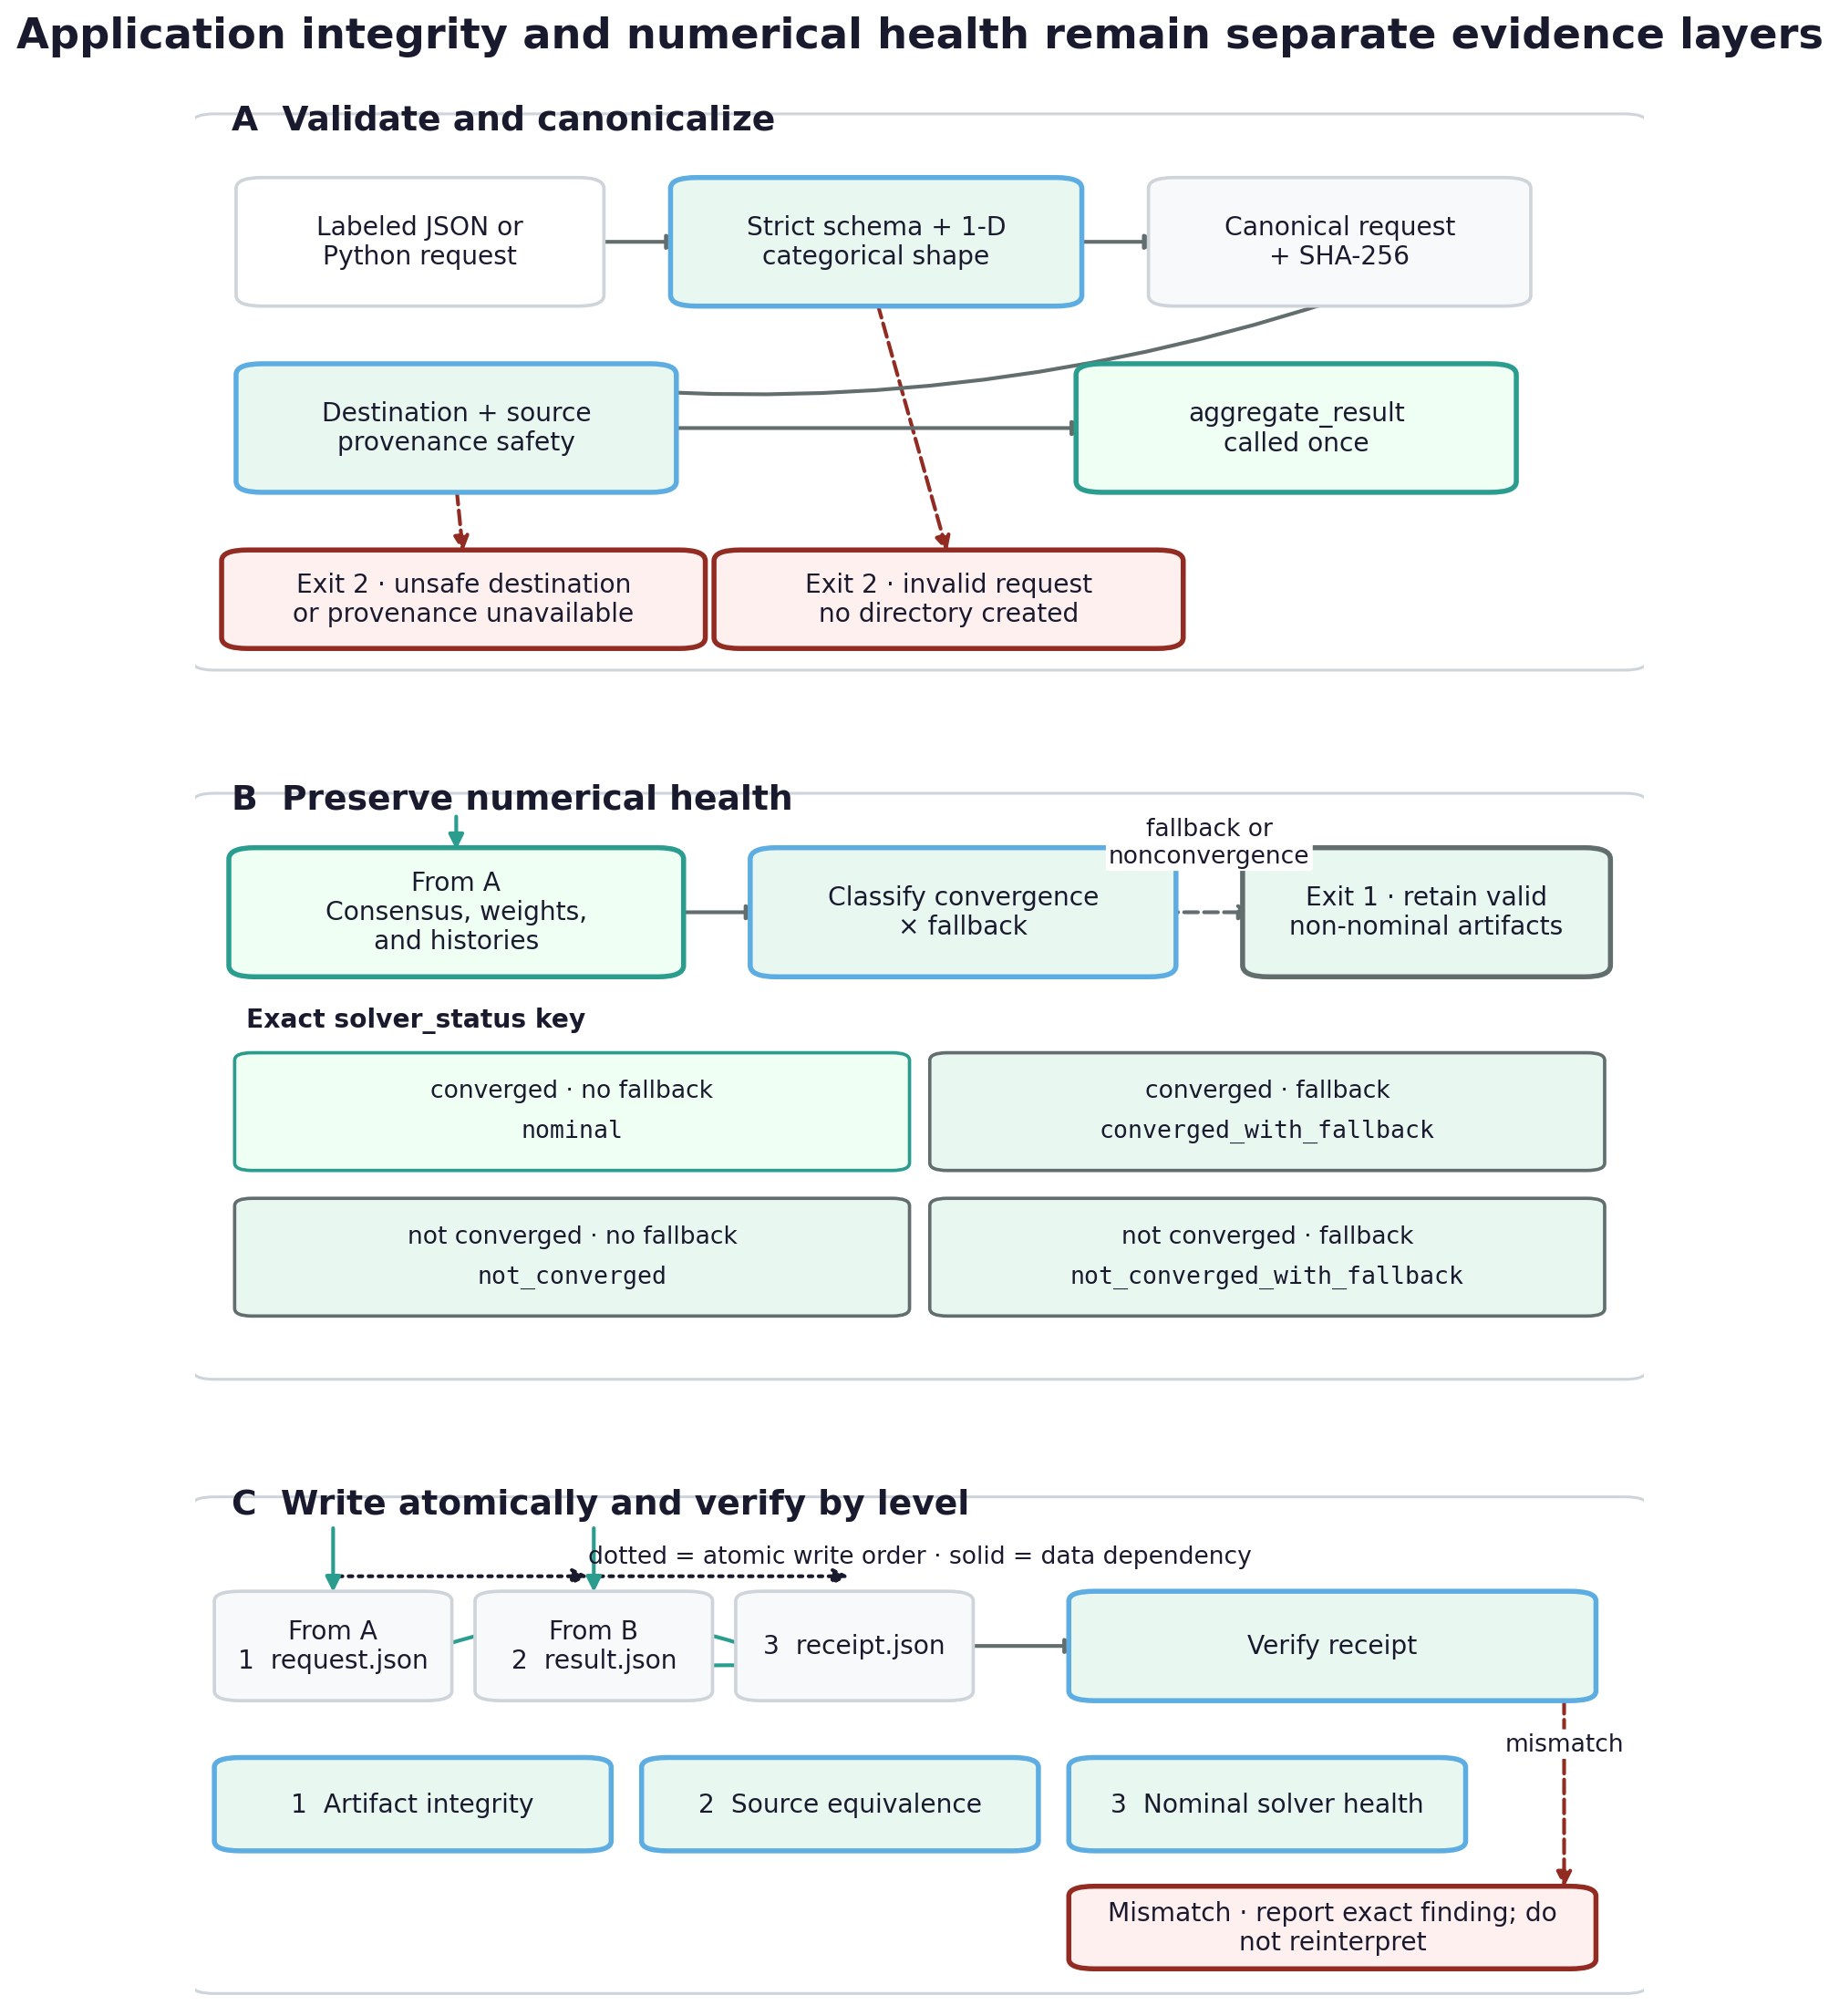
\includegraphics[width=0.95\linewidth,height=0.5\textheight,keepaspectratio,alt={Three vertical panels show request validation and canonical hashing, a two-by-two key for the four exact solver\csname char_generate:nn\endcsname{95}{12}status codes, and atomic request/result/receipt writing with a separate three-level verification lane. Red dashed exits reject invalid input or report mismatches; a neutral dashed exit retains non-nominal results.}]{../figures/application_integrity_flow.png}
\caption{The labeled application path separates fail-closed request and
destination checks from retained non-nominal results. Source relation:
source-owned labeled-aggregation, solver-health, artifact, and receipt
contracts; status: deterministic implementation map, not an experiment.
Panel A follows labeled JSON or Python input through strict schema and
one-dimensional shape validation, canonical semantic hashing, a
destination-and-required-provenance safety gate, and one delegation to
the shared aggregation result. Its two dashed rejection branches
distinguish an invalid request from an unsafe destination or unavailable
required provenance; both exit 2 before directory creation. Panel B
classifies convergence and fallback state, then gives the exact
two-by-two \protect\texttt{solver\_status} key:
\protect\texttt{nominal}, \protect\breaktt{converged\_with\_fallback},
\protect\texttt{not\_converged}, and
\protect\breaktt{not\_converged\_with\_fallback}. Panel C carries the
canonical request and rich result into \protect\texttt{request.json} and
\protect\texttt{result.json}, binds both into
\protect\texttt{receipt.json}, and enters verification. Solid arrows
encode data dependency; the dotted sequence records atomic write order;
dashed paths mark rejection or a retained warning. The x-axis is
left-to-right execution within rows; rows order panels and verification
levels. The estimand is validation, artifact, and solver state; the unit
is one categorical software state per invocation. No sampling
uncertainty or independent replication unit applies. Exit 1 retains
non-nominal artifacts, and a mismatch reports its exact finding. Receipt
integrity, source equivalence, and nominal health do not establish
calibration, domain suitability, scientific validity, downstream
decision correctness, or
acceptance.}\label{fig:application-integrity-flow}
\end{figure}

\subsection{Environment fingerprint for the reported
run}\label{sec:repro-environment}

The second reproduction input is the exact toolchain. Every field below
is captured by the successful full test-and-coverage receipt before
final variable generation rather than transcribed by hand. The receipt
is bound to the source, tests, manuscript, source-owned documentation,
release metadata, ISC tree, dependency lock, and fresh analysis receipt.

It rejects any pre/post-suite drift in that boundary, so a reader
matching this environment and the seed above can reproduce the seeded
results; the config hash lets them confirm they are running the
configuration from which this manuscript was rendered.

\begin{longtable}[]{@{}ll@{}}
\caption{Software and configuration fingerprint for the hydrated
manuscript. The build epoch is derived from
\protect\breaktt{SOURCE\_DATE\_EPOCH}; an unreleased build records an
explicit omitted sentinel rather than wall-clock
time.}\label{tbl:repro_env}\tabularnewline
\toprule\noalign{}
Field & Value \\
\midrule\noalign{}
\endfirsthead
\toprule\noalign{}
Field & Value \\
\midrule\noalign{}
\endhead
\bottomrule\noalign{}
\endlastfoot
Python & 3.12.12 \\
NumPy & 2.4.2 \\
SciPy & 1.18.0 \\
PyTorch (MLP complement) & 2.12.1 \\
Platform & Darwin arm64 \\
Config hash (SHA-256, first 16) & cbe919be0d1d3903 \\
Reproducible build epoch (UTC) & 2026-09-13T01:42:53Z \\
\end{longtable}

The exact environment used for the reported run is recorded in
tbl.~\ref{tbl:repro_env}.

\subsection{Reader-surface accessibility
boundary}\label{sec:repro-accessibility}

The validated HTML manuscript is the canonical accessibility-enhanced
reading surface. Its source gate requires a page language and title, a
skip link and main landmark, non-empty image alternatives, figure
captions, labelled full-size links, unique identifiers, resolved
references, and present local assets on every generated page.

These deterministic checks are not a claim of WCAG conformance:
alternative-text quality, contrast, keyboard behavior, reading order,
reflow, mathematics, and assistive-technology behavior still require
manual review.

The combined manuscript PDF is generated through the source-controlled
LuaLaTeX/tagpdf path and is released only when \texttt{pdfinfo} reports
\texttt{Tagged:\ yes}, qpdf exposes a non-empty \texttt{/Lang} and
\texttt{StructTreeRoot}, and the source-bound language check passes.

Some Poppler builds omit the language line from \texttt{pdfinfo} even
when \texttt{/Lang} is present. The separate slide PDFs are checked
structurally, textually, through renderer logs during the producing run,
and by raster inspection, but do not inherit the manuscript tagging
status. Renderer logs are retained with the external verification
evidence rather than the public source tree because they contain
environment-local timestamps and paths.

Tagged structure is not PDF/UA conformance: a PDF/UA claim requires a
dedicated conformance report plus screen-reader and reading-order
review; \texttt{qpdf} structure checks and successful text extraction
alone are insufficient.

\subsection{Test and coverage evidence for the claim
surface}\label{sec:repro-tests}

\textbf{Acceptance criteria.} 268 total, 266 passing.

\textbf{Project test suite.} 2847 collected cases; the bound successful
receipt records zero failed cases. The project no-mocks policy remains a
separately executable source contract.

\textbf{Combined line and branch coverage on \texttt{src/}.} 90.57\%,
achieved by the bound full gate with branch measurement enabled. The
shared coverage threshold is \(\ge 90\%\) on this combined measure.

To regenerate this evidence from a clean checkout, run the project suite
under the pinned development environment. Local execution and hosted CI
are separate results; the hosted checks must pass for the exact reviewed
commit before public integration. Both use the following coverage gate:

\begin{Shaded}
\begin{Highlighting}[]
\ExtensionTok{uv}\NormalTok{ run }\AttributeTok{{-}{-}locked} \AttributeTok{{-}{-}extra}\NormalTok{ dev pytest tests/ }\DataTypeTok{\textbackslash{}}
  \AttributeTok{{-}{-}cov}\OperatorTok{=}\NormalTok{src }\AttributeTok{{-}{-}cov{-}fail{-}under}\OperatorTok{=}\NormalTok{90}
\end{Highlighting}
\end{Shaded}

For a release-facing hydration, use the receipt-producing wrapper after
any required provisional pre-test render, then rerun hydration without
its provisional flag:

\begin{Shaded}
\begin{Highlighting}[]
\ExtensionTok{uv}\NormalTok{ run }\AttributeTok{{-}{-}locked} \AttributeTok{{-}{-}extra}\NormalTok{ dev python scripts/validate\_test\_coverage.py}
\ExtensionTok{uv}\NormalTok{ run }\AttributeTok{{-}{-}locked}\NormalTok{ python scripts/}\DataTypeTok{\textbackslash{}}
\NormalTok{z\_generate\_manuscript\_variables.py}
\end{Highlighting}
\end{Shaded}

\subsection{Artifact inventory for figures, data, and
reports}\label{sec:repro-artifacts}

\begin{longtable}[]{@{}ll@{}}
\caption{Top-level generated files in \protect\texttt{output/figures},
\protect\texttt{output/data}, and \protect\texttt{output/reports} at
token-hydration time. The generated release manifest is the source of
truth for the larger recursive publication bundle. Artifacts are
regenerable reviewer snapshots and must not be
hand-edited.}\label{tbl:repro_artifacts}\tabularnewline
\toprule\noalign{}
Category & Count \\
\midrule\noalign{}
\endfirsthead
\toprule\noalign{}
Category & Count \\
\midrule\noalign{}
\endhead
\bottomrule\noalign{}
\endlastfoot
Figures & 1226 \\
Data files & 5 \\
Reports & 36 \\
Total & 1267 \\
\end{longtable}

The top-level artifact counts in tbl.~\ref{tbl:repro_artifacts}
complement the recursive, checksum-bearing release manifest.

\section{Reproducibility: producer provenance and recovery
checks}\label{sec:repro-production}

\subsection{Producer order, stale invalidation, and publication
authority}\label{sec:repro-provenance-map}

The provenance map in fig.~\ref{fig:source-render-provenance} records
the source-owned producer contract rather than inferring it from the
release manifest. Panel A places the non-sequential fan-in dependencies
in a labeled matrix, then orders the temporal, gate, receipt, and
authorization dependencies in a crossing-free process path. Source,
configuration, lockfile, figure-accessibility registries, and the exact
clean Template commit remain explicit inputs.

Panel B's fourteen coded dashed cards make reverse invalidation explicit
without crossing the forward process path. Each arrow starts at one or
more immediate stale targets on the right and points back to its changed
owner on the left. A changed owner makes the named immediate targets and
their downstream reports, figures, hydrated text, rendered surfaces,
provenance, and release receipts stale; previously green bytes are not
carried forward.

GitHub and Zenodo are terminal authorization states, not automatic
products of a green build. The figure itself is generated from the
source-owned pipeline contract and never reads the downstream release
manifest that later inventories it, avoiding a circular dependency.

\begin{figure}
\centering
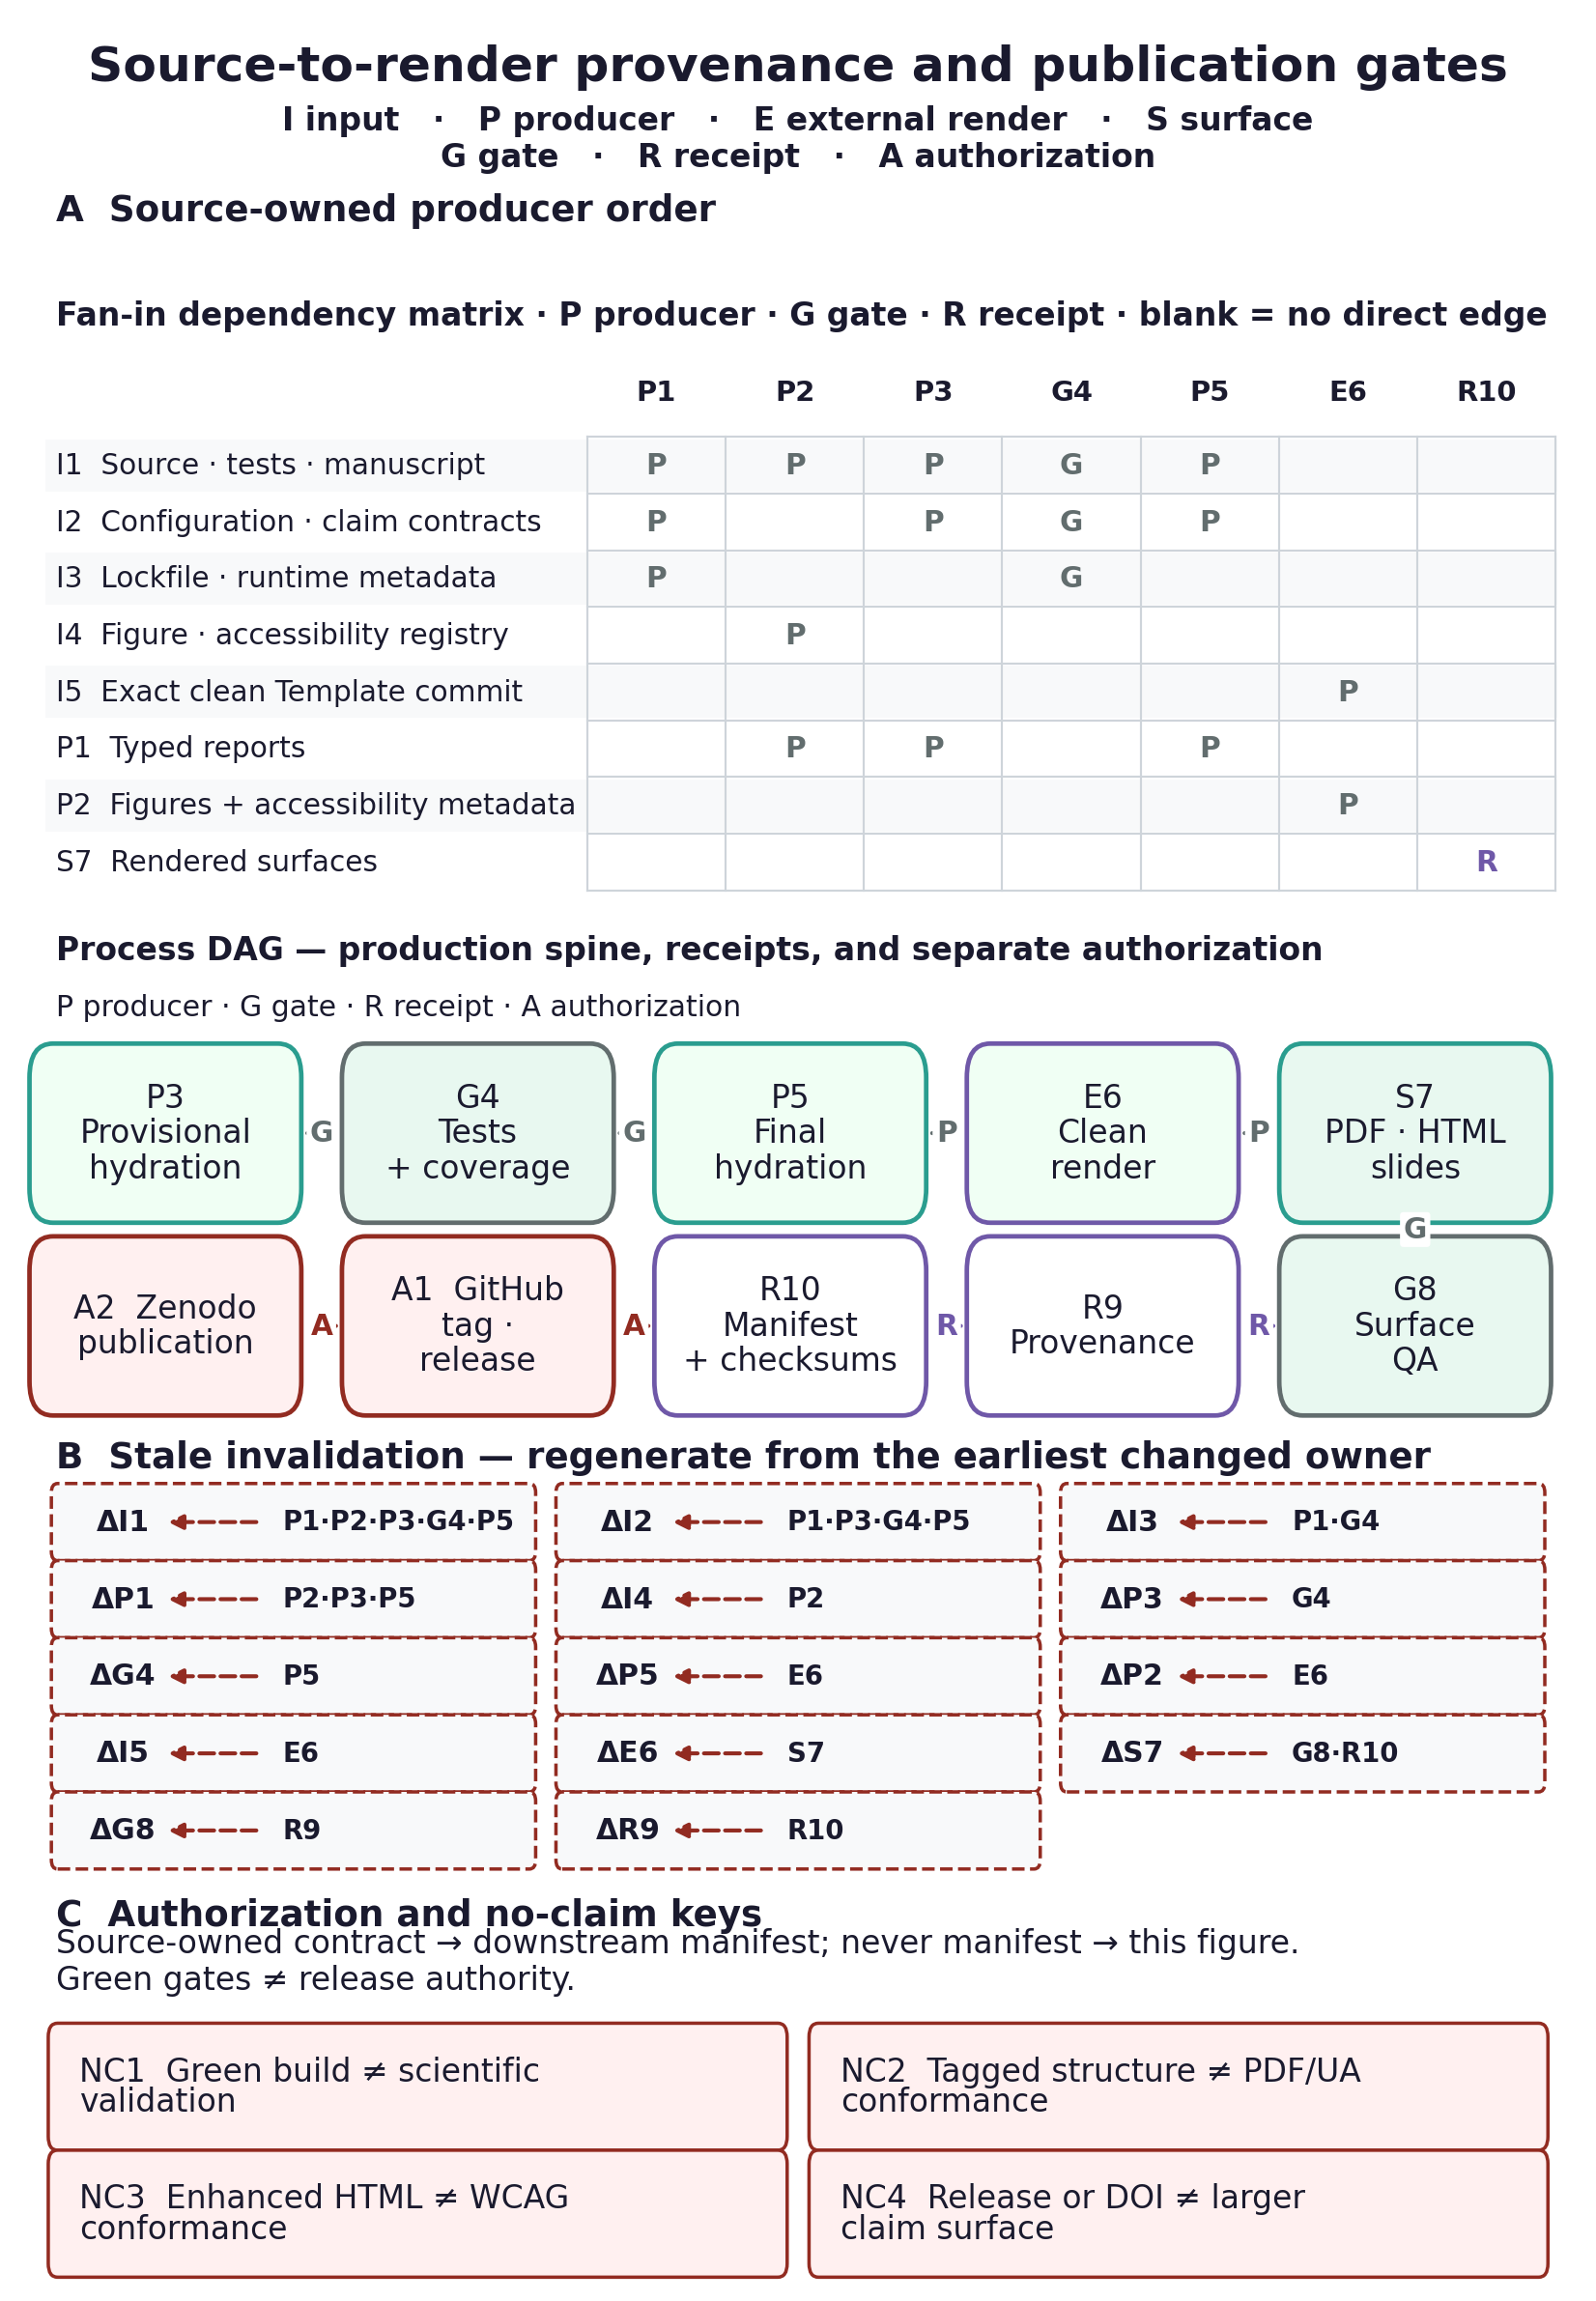
\includegraphics[width=0.95\linewidth,height=0.5\textheight,keepaspectratio,alt={Three vertical panels show a five-input dependency matrix beside a crossing-free producer path, fourteen reverse-invalidation cards, and cycle and authorization boundaries. Letter codes and arrows duplicate color; GitHub and Zenodo remain separately authorized terminal states.}]{../figures/source_render_provenance.png}
\caption{Publication surfaces inherit source state; green gates remain
distinct from release authority. Source relation: source-owned
explanatory producer and invalidation contract; study status:
deterministic provenance map, not an empirical result. Read Panel A
first across the dependency matrix and then through the two-band process
path. The matrix x-axis indexes seven downstream targets, while its rows
name five inputs and three upstream producers; each populated cell
carries a producer, gate, or receipt code. The adjacent crossing-free
path orders provisional hydration, tests and coverage, final hydration,
exact clean Template rendering, reader surfaces, surface checks,
provenance, manifests, and the separately authorized GitHub and Zenodo
terminals. Panel B groups fourteen changed owners into dashed
reverse-dependency cards; each arrow points from immediate stale targets
back to its changed owner. Panel C states the non-circular manifest
boundary and four no-claim rules. Codes, direct labels, keylines, solid
producer or receipt arrows, dashed gate arrows, and dashed reverse
arrows duplicate color. The estimand is categorical dependency and
authorization state; the unit is one pipeline or publication stage.
There is no sampling uncertainty, sample size, or replication unit. The
figure never reads the downstream manifest. A green build does not
authorize publication, establish scientific validity, PDF/UA or WCAG
conformance, or enlarge the claim surface through a release or
DOI.}\label{fig:source-render-provenance}
\end{figure}

\subsection{Recovery-limit certificate for the client and project-pool
corners}\label{sec:repro-recovery}

The recovery identities are reproducibility checks: the client machinery
must return to standard Bayes at its KL/NLL loss limits, and the server
heuristic must return to the project's log-linear pool at zero
robustness (eq.~\ref{eq:robust-identity}, eq.~\ref{eq:standard-bayes}).

Under the explicit shared-support, posterior-log-potential, and
fixed-weight assumptions of sec.~\ref{sec:method-aggregation}, that pool
specializes Eq. 7's message-combination term; it does not reproduce the
complete source protocol. These deviations are computed on every build.

\textbf{Server recovery:} \breaktt{robust\_aggregate(robustness=0)}
versus \texttt{log\_linear\_pool} (eq.~\ref{eq:log-linear-pool}) has
maximum difference 0.

\textbf{Posterior recovery:} \breaktt{generalized\_posterior(KLD,\ NLL)}
versus closed-form Bayes has maximum difference 5.55e-17.

\textbf{Divergence recovery:} Rényi divergence versus KL as
\(\alpha\to 1\) has maximum difference 0.

\textbf{Loss recoveries:} \(\beta\)-loss versus NLL as \(\beta\to 0\)
has maximum difference 0, while rcce versus NLL as
\(q_{\text{loss}}\to 0\) has maximum difference 0.

Any drift in these limits beyond machine precision would mean the robust
generalization no longer contains its standard-Bayes client limit and
project-local log-linear-pool server limit
(sec.~\ref{sec:results-recovery}) --- and would fail the core test suite
before this certificate could render.

The certificate covers the recovery identity and the client-side result
under the cited source theorem's matching assumptions only; the
server-side \breaktt{robust\_aggregate} heuristic is certified here for
its recovery limit alone, not for any bounded-influence property
(sec.~\ref{sec:limitations}).

All code is authored by Daniel Ari Friedman and licensed under the MIT
license. This is project version 1.1.0.dev0.

\section{Supplement: variational aggregation objective and weight
control}\label{sec:supp-variational}

\ifcsname proposition\endcsname
\else
\newtheorem{proposition}{Proposition}
\fi

This supplement gives the full derivation behind
sec.~\ref{sec:method-variational}: the server-side aggregator
\breaktt{robust\_aggregate} is a heuristic, and a single change of
divergence direction turns it into block-coordinate descent on a stated
free energy with a derived, redescending effective-weight update.

We work throughout with categorical local posteriors \(q_n(s)\) over the
shared latent factor, base weights \(w_n > 0\), robustness \(c > 0\),
and the consensus \(q\) on the probability simplex. Let \(\lambda>0\) be
the entropy-weight coefficient, with the current default at
\(\lambda=1.0\).

\subsection{Why the sharp heuristic is not yet
variational}\label{sec:supp-why-heuristic}

The sharp server rule is empirically strong, but this repository has not
established a variational certificate for it. The heuristic of
eq.~\ref{eq:robust-identity} alternates a \emph{reverse-KL} weight
update \(a_n \leftarrow w_n\exp(-c\,\mathrm{KL}(q_n \,\|\, q))\).

It couples that update with the log-linear consensus
\(q \leftarrow \mathrm{softmax}(\sum_n a_n \log q_n)\). For the natural
direct objective \(\sum_n a_n \mathrm{KL}(q_n \,\|\, q) +
\tfrac{1}{c}\mathrm{KL_{gen}}(a\,\|\,w)\), the reverse-KL rule is the
\(a\)-minimizer.

The \(q\)-minimizer is the \emph{arithmetic} (linear) pool
\(q \propto \sum_n a_n q_n\), not the log-linear pool. The executable
orientation witness confirms this finite-simplex mismatch. The following
proposition goes further, while retaining a deliberately narrow scope.

\begin{equation}\protect\phantomsection\label{eq:raw-log-pool-block}{
Q(a;s) \;=\; \operatorname{softmax}\!\left(\sum_n a_n\log s_n\right)
}\end{equation}

The proposed raw \(q\)-block is the map in
eq.~\ref{eq:raw-log-pool-block}.

\begin{equation}\protect\phantomsection\label{eq:separable-server-objective}{
\begin{aligned}
F(q,a;s,w)
&= \sum_n a_n\,\mathrm{KL}(q\,\|\,s_n)\\
&\quad + R(a,w) + G(q).
\end{aligned}
}\end{equation}

\begin{proposition}[Scoped separable raw-log-pool no-go]\label{prop:raw-log-pool-no-go}
For \(K\geq2\), no objective in (\ref{eq:separable-server-objective}) satisfying
the declared separability and differentiability conditions has \(Q(a;s)\) as
its \(q\)-coordinate minimizer for every positive interior \(a\) and \(s\).
\end{proposition}

Precisely, \(G\) is continuously differentiable and independent of
\(a,s\), while \(R\) is independent of \(q,s\). Under those conditions,
this objective class cannot realize both block maps of the implemented
raw-weight heuristic.

\emph{Proof sketch.} Fix any non-uniform interior \(q\), a positive
scalar \(\alpha\), and one local posterior constructed in
eq.~\ref{eq:raw-log-pool-witness-source}:

\begin{equation}\protect\phantomsection\label{eq:raw-log-pool-witness-source}{
s_i^{(\alpha)} \;=\;
\frac{q_i^{1/\alpha}}{\sum_j q_j^{1/\alpha}}.
}\end{equation}

Then \(Q(\alpha;s^{(\alpha)})=q\). Writing \(\Pi\) for projection onto
the tangent space of the simplex, first-order stationarity of
eq.~\ref{eq:separable-server-objective} at that same \(q\) requires
\(\Pi[(\alpha-1)\log q+\nabla G(q)]=0\).

The unit-scale construction forces \(\Pi\nabla G(q)=0\); any different
positive scale then forces \(\Pi\log q=0\), contradicting the
non-uniform choice of \(q\). The executable witness records both exact
log-pool identities and the nonzero tangential contradiction.

A companion witness also blocks the obvious normalized-weight escape
within the same natural data-term class: two interior consensuses yield
the same normalized reverse-KL weights but different forward-KL
data-term differences, so a \(q\)-independent differentiable \(R(a,w)\)
cannot satisfy both simplex-stationarity equations. The implementation
itself uses raw effective weights, so this companion is a scope check
rather than a description of the production update.

\begin{longtable}[]{@{}
  >{\raggedright\arraybackslash}p{(\linewidth - 2\tabcolsep) * \real{0.5000}}
  >{\raggedright\arraybackslash}p{(\linewidth - 2\tabcolsep) * \real{0.5000}}@{}}
\caption{Formal MAJ-1 witness inventory. These are deterministic
finite-simplex proof artifacts, not empirical estimates; no resampling
interval or deployment claim is
implied.}\label{tbl:server-theory-witness}\tabularnewline
\toprule\noalign{}
\begin{minipage}[b]{\linewidth}\raggedright
Artifact
\end{minipage} & \begin{minipage}[b]{\linewidth}\raggedright
Implementation surface and declared scope
\end{minipage} \\
\midrule\noalign{}
\endfirsthead
\toprule\noalign{}
\begin{minipage}[b]{\linewidth}\raggedright
Artifact
\end{minipage} & \begin{minipage}[b]{\linewidth}\raggedright
Implementation surface and declared scope
\end{minipage} \\
\midrule\noalign{}
\endhead
\bottomrule\noalign{}
\endlastfoot
Raw contradiction & \breaktt{server\_theory.py}; interior inputs and raw
\(q\)-block \\
Normalized companion & \breaktt{server\_theory.py}; forward-KL class and
normalized weights \\
Typed report & \texttt{formal\_no\_go}; witness metadata, with the
attack grid kept separate \\
\end{longtable}

The witness table in tbl.~\ref{tbl:server-theory-witness} records the
deterministic implementation surfaces that bind this scoped result to
the typed analysis report.

The proposition does \textbf{not} say that no objective of any kind
exists. It does not exclude nonseparable \(q\)--\(a\) couplings,
source-dependent terms, non-differentiable constructions, or objectives
that encode selected fixed points without reproducing the update blocks
for all interior inputs. Thus sec.~\ref{sec:method-aggregation} retains
the heuristic label and claims only the recovery limit, the scoped
negative result above, and conditional empirical behavior --- never a
bounded-influence property or an objective-backed status.

\subsection{Aggregation free energy and its block
minimizers}\label{sec:supp-derivation}

\begin{definition}[Aggregation free energy]\label{def:aggregation-free-energy}
For \(c,\lambda>0\), consensus \(q\), and nonnegative effective weights
\(a=(a_n)\), define \(F_\lambda(q,a)\) by (\ref{eq:agg-free-energy}), where
\(\mathrm{CE}(q,q_n)=-\sum_i q_i\log q_{n,i}\), \(H(q)\) is entropy, and
\(\mathrm{KL}_{\rm gen}(a\|w)=\sum_n g_n\) for
\(g_n=a_n\log(a_n/w_n)-a_n+w_n\).
\end{definition}

\textbf{The \(q\)-block.} For \(\lambda>0\), fixing \(a\), the
\(q\)-dependent part of \(F_\lambda\) is denoted \(J(q;a)\) and can be
written in either of two equivalent forms:

\begin{equation}\protect\phantomsection\label{eq:agg-q-objective}{
\begin{aligned}
J(q;a)
&=\sum_n a_n\,\mathrm{CE}(q,q_n)-\lambda H(q),\\
J(q;a)
&=\lambda\sum_i q_i\log q_i\\
&\quad-\sum_i\sum_n q_i a_n\log q_{n,i}.
\end{aligned}
}\end{equation}

Adding a Lagrange multiplier to the block in
eq.~\ref{eq:agg-q-objective} for \(\sum_i q_i = 1\) and differentiating
gives \(\lambda\log q_i + \lambda - \sum_n a_n \log q_{n,i} + \mu = 0\),
i.e.

\begin{equation}\protect\phantomsection\label{eq:agg-q-min}{
\begin{aligned}
q_i
&\propto \exp\!\Big(
  \tfrac{1}{\lambda}\sum_n a_n \log q_{n,i}\Big),\\
q_i
&= \mathrm{softmax}\!\Big(
  \tfrac{1}{\lambda}\sum_n a_n \log q_n\Big)_i.
\end{aligned}
}\end{equation}

the product of the weighted experts --- the consensus update of
eq.~\ref{eq:agg-updates}. At the default \(\lambda=1.0\), the \(-H(q)\)
term sharpens the weighted geometric mean into the product-of-experts
(the entropy bonus that makes the project's log-linear pool a product
rather than a geometric average).

\textbf{The \(a\)-block.} Fixing \(q\),
\(\partial F/\partial a_n = \mathrm{CE}(q,q_n) + \tfrac{1}{c}\log(a_n/w_n) = 0\),
so

\begin{equation}\protect\phantomsection\label{eq:agg-a-min}{
a_n \;=\; w_n\,\exp\!\big(-c\,\mathrm{CE}(q, q_n)\big),
}\end{equation}

the weight update of eq.~\ref{eq:agg-updates}. Because
\(\mathrm{CE}(q,q_n) = H(q) + \mathrm{KL}(q\,\|\,q_n)\), the forward
direction \(\mathrm{KL}(q\,\|\,q_n)\) --- not the heuristic's reverse
\(\mathrm{KL}(q_n\,\|\,q)\) --- is the one consistent with the consensus
update.

Each block update is the \emph{exact} minimizer of its block, so
alternating them is block-coordinate descent: \(F\) is non-increasing at
every half-step. When the iterates converge, their fixed point is
coordinatewise stationary.

The implementation keeps numerical failure handling outside that
theorem. If finite-precision underflow collapses all effective weights,
it records a fallback event, substitutes the declared base weights to
return a valid probability vector, and does not certify the substituted
trajectory as converged. Such a trace is diagnostic evidence about the
solver boundary, not an instance of the exact block-descent result.

\subsection{Conservative-server properties}\label{sec:supp-theorem}

\begin{theorem}[Properties]
\label{thm:variational-aggregation}
For \(c,\lambda>0\), (\ref{eq:agg-q-min})–(\ref{eq:agg-a-min}) make \(F\)
non-increasing. At convergence, \((q^*,a^*)\) is coordinatewise stationary.
As \(c\to0\), \(a_n\to w_n\) and \(q\) tends to the tempered log-linear pool;
\(\lambda=1.0\) gives
(\ref{eq:log-linear-pool}). Finally,
\(a_n=w_n\exp[-c\,\mathrm{CE}(q,q_n)]\le w_n\), and
\(\mathrm{KL}(q\,\|\,q_n)\to\infty\) gives \(a_n\to0\).
\end{theorem}

The variational aggregator therefore shares the project log-linear-pool
corner of (\ref{eq:robust-identity}). Under the qualified bridge of
sec.~\ref{sec:method-aggregation}, this is only the categorical
message-combination specialization, not the complete source protocol.

The final inequality makes the raw effective-weight update bounded and
redescending relative to the realized consensus. It does not by itself
establish a bounded influence function or finite gross-error sensitivity
for the normalized consensus estimator.

The objective \(F\) is biconvex (each block convex, the coupling
\(\sum_n a_n\mathrm{CE}(q,q_n)\) bilinear), so the result concerns
monotone block updates and converged coordinatewise fixed points, not
guaranteed convergence to or certification of a global minimum.

\textbf{The effective-weight regime, and why multi-start matters.} The
weight bound \(a_n \le w_n\) is unconditional
(\(\mathrm{CE}(q,q_n)\ge 0\) always). The \emph{collapse} \(a_n \to 0\)
is driven by the agent's divergence \emph{from the realized consensus}
\(\mathrm{KL}(q\,\|\,q_n)\), and the consensus itself depends on the
weights.

Because \(F\) is biconvex, this couples into a subtlety an adversarial
review of this work surfaced: a \emph{near-one-hot} saboteur
(contamination rate \(\to 1\)) already captures the product-of-experts,
so a descent seeded \emph{at} that pool stays in a consensus-capture
basin (high \(F\)) where the saboteur keeps its weight --- even against
an honest majority.

The repair is to search the stated objective more carefully:
\breaktt{variational\_aggregate} runs \textbf{multi-start}
block-coordinate descent (the pool, the uniform belief, and the
arithmetic-mean seeds) and returns the lowest-observed-\(F\) converged
candidate.

In the configured colony, the uniform/arithmetic seeds reach a
lower-\(F\) \emph{vetoing} basin, so the saboteur is suppressed even at
the simplex vertex (pinned qualitatively by the near-vertex multi-start
test) --- the 267.1\(\times\) suppression of
fig.~\ref{fig:bounded-influence} is measured across the swept
contamination grid, whose most extreme point sits just below rate \(1\).

What remains fundamental to \emph{every} robust fusion rule, and is not
claimed away: with no honest majority --- a colony split with no
anchoring plurality --- there is no truth to recover.

The observed suppression is conditional on the tested colonies and the
fixed point selected by a finite multi-start heuristic.

fig.~\ref{fig:descent-comparison} makes the capture and the escape
concrete on a near-vertex colony: the single (log-linear-pool) start
settles at \(F = 1.3092\) (the higher observed basin, where the saboteur
keeps its weight), while one of the configured alternative starts
reaches a lower observed basin at \(F = -0.2305\) --- a gap of 1.5397
nats. This finite multistart comparison shows that the natural seed can
be captured; it neither exhausts all basins nor certifies a global
optimum.

\begin{figure}
\centering
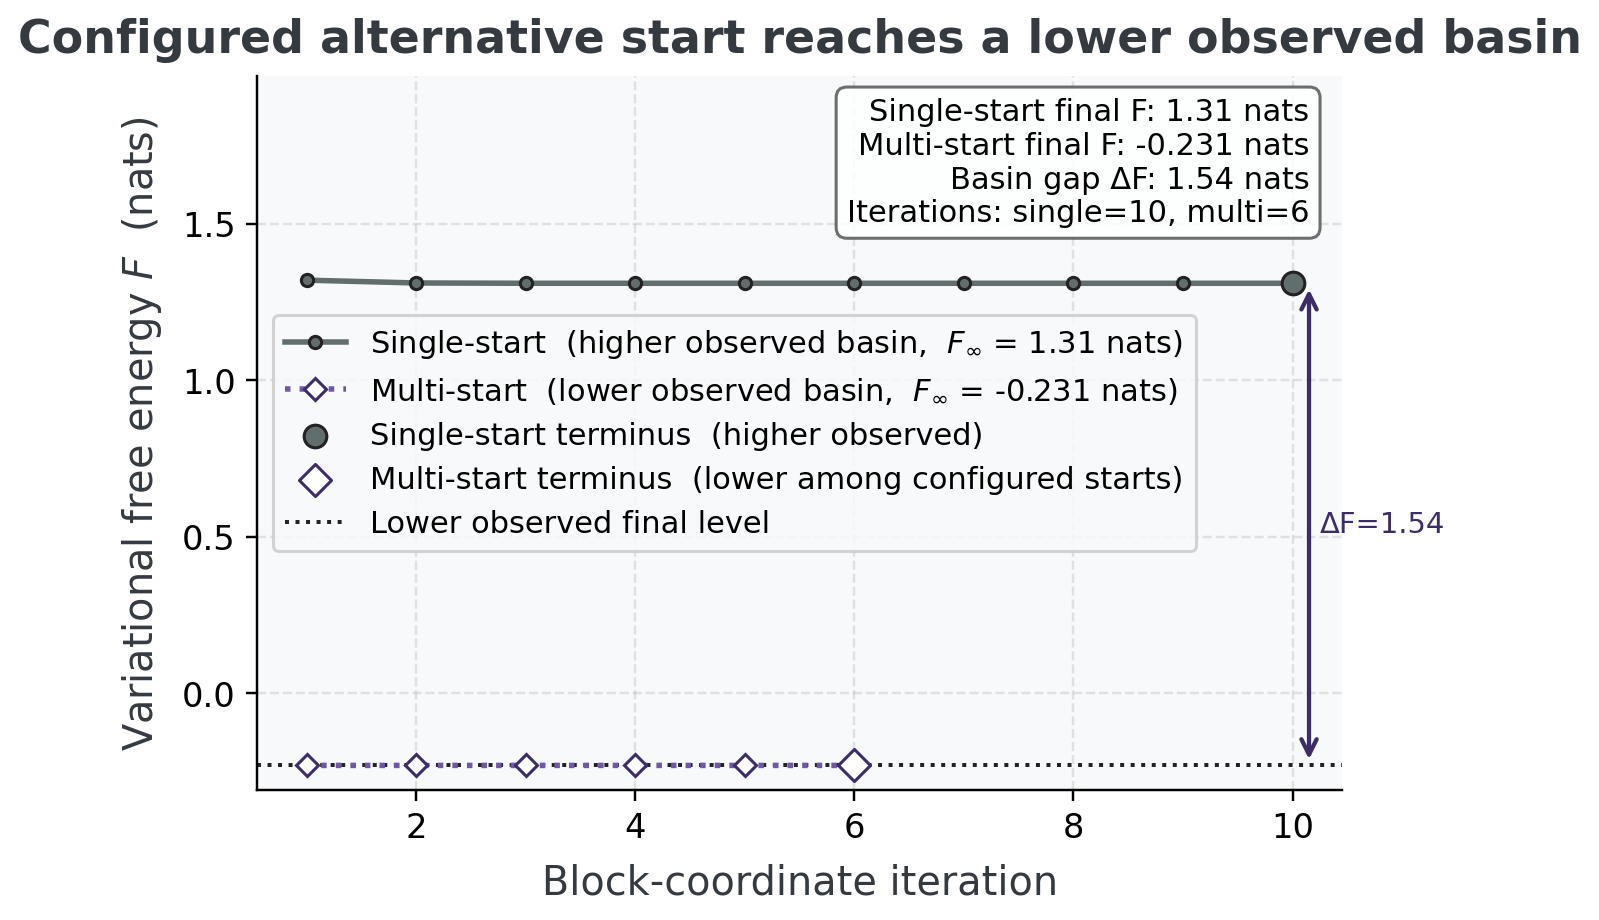
\includegraphics[width=0.8\linewidth,height=0.5\textheight,keepaspectratio,alt={A filled-circle solid path and an open-diamond dotted path compare single-start and multistart variational free-energy descent as neutral initialization conditions. The single start remains in a higher observed basin; a dark dotted rule marks the lower multistart terminal level.}]{../figures/descent_comparison.png}
\caption{Variational free-energy descent on a near-vertex adversarial
colony. Source relation: original project objective-descent diagnostic;
estimand: objective value \(F\) in nats by block-coordinate iteration
and configured initialization. The x-axis is iteration and the y-axis is
\(F\). A filled-circle solid path marks the single-start condition and
an open-diamond dotted path marks the multistart condition; these
neutral condition encodings do not imply different aggregation methods.
Directly labeled terminal marks identify the higher and lower observed
basins, a dark dotted rule marks the lower observed final level, and a
double-ended annotation reports the terminal gap. The log-linear-pool
single start settles at \(F=1.3092\) with retained saboteur weight,
whereas the lowest trajectory among the configured alternatives reaches
\(F=-0.2305\), a gap of 1.5397 nats. These are two deterministic traces
from one configured colony, not independent stochastic replications, so
no error bar, confidence interval, or resampling interval applies.
Finite multistart descent does not certify a global optimum, enumerate
every basin, or establish universal
robustness.}\label{fig:descent-comparison}
\end{figure}

\subsection{Numerical witnesses for descent and influence
bounds}\label{sec:supp-witnesses}

The analysis pipeline runs \breaktt{variational\_aggregate} at robustness
\(c = 1.50\) on a contaminated colony and records the free energy after
each iteration. The descent falls from \(F = 3.2458\) to \(F = 2.3780\)
(a monotone drop of \(0.8678\) over 11 iterations, converged: Yes); the
largest single-step \emph{increase} is \(8.88 \times 10^{-16}\), machine
zero --- the monotonicity of the theorem, witnessed numerically and
drawn in fig.~\ref{fig:aggregation-descent}.

For the effective-weight diagnostic, one agent is drifted from healthy
toward a confident-wrong delta and its normalized influence is read at
each drift. Clean, it carries \(0.143\) of the pool; at the most extreme
swept drift it carries below \(0.001\) --- a factor of 267.1 (computed
from the unrounded influences, not the display-rounded values above)
below the fixed 0.143 the naive pool would still grant it
(fig.~\ref{fig:bounded-influence}).

This makes the redescending normalized-weight behavior visible on the
tested path; it is not an estimator-level B-robustness proof.

\subsection{Tempered aggregation family for the accuracy-guarantee
trade}\label{sec:supp-tempered}

The aggregator of sec.~\ref{sec:supp-derivation} fixes the entropy term
at unit weight. Relaxing that single coefficient generates a
one-parameter \emph{tempered} family. Introduce an entropy weight
\(\lambda > 0\) --- the \textbf{inverse temperature is} \(1/\lambda\)
--- and minimize

\begin{equation}\protect\phantomsection\label{eq:tempered-family}{
\begin{aligned}
F_\lambda(q, a)
&= \sum_n a_n\,\mathrm{CE}(q, q_n) - \lambda H(q)\\
&\quad + \tfrac{1}{c}\,\mathrm{KL_{gen}}(a \,\|\, w).
\end{aligned}
}\end{equation}

Repeating the \(q\)-block derivation of eq.~\ref{eq:agg-q-min} with the
entropy scaled by \(\lambda\) leaves the \(a\)-block \textbf{untouched}
and tempers only the consensus update:

\begin{equation}\protect\phantomsection\label{eq:tempered-updates}{
\begin{aligned}
q
&\propto \exp\!\Big(
  \tfrac{1}{\lambda}\textstyle\sum_n a_n \log q_n\Big),\\
a_n
&= w_n\,\exp\!\big(-c\,\mathrm{CE}(q, q_n)\big).
\end{aligned}
}\end{equation}

The \(\lambda\downarrow0\) endpoint is separately implemented as a
deterministic tied-argmax rule; it is not obtained by substituting
\(\lambda=0\) into eq.~\ref{eq:tempered-family} or
eq.~\ref{eq:tempered-updates}.

The weight update is \textbf{independent of \(\lambda\)}: the bound
\(a_n \le w_n\) with collapse \(a_n \to 0\) as
\(\mathrm{KL}(q\,\|\,q_n) \to \infty\) is unchanged, so the \textbf{raw
effective-weight bound of sec.~\ref{sec:supp-theorem} holds for every}
\(\lambda > 0\). At \(\lambda = 1.0\) the temperature is unity and
eq.~\ref{eq:tempered-updates} is \textbf{identical} to the current
axis-3 aggregator eq.~\ref{eq:agg-updates} --- the default is
bit-identical, not merely close.

The \(c \to 0\) recovery of sec.~\ref{sec:supp-theorem} generalizes to
the \emph{tempered} log-linear pool
\(q \propto \exp(\tfrac{1}{\lambda}\sum_n w_n \log q_n)\); at
\(\lambda = 1.0\) this is exactly
\(\mathrm{softmax}(\sum_n w_n \log q_n)\) --- the project's
\textbf{log-linear pool} eq.~\ref{eq:log-linear-pool}.

Under the shared-support, posterior-log-potential, and fixed-weight
assumptions of sec.~\ref{sec:method-aggregation}, that pool is a
categorical specialization of Friston Eq. 7's message-combination term,
not a reconstruction of the complete source protocol.
Positive-temperature members away from that default are tempered pools,
not Friston Eq. 7 itself; the project recovery checks, including ISC-10,
remain project-local.

A small empirical sweep over
\(\lambda \in \{ 0.1, 0.2, 0.3, 0.5, 0.7, 1 \}\) on 10 contaminated
colonies (5 agents, 2 adversarial) asks whether a single
\(\lambda^{\ast}\) makes the conservative aggregator narrow the gap to
the sharp \(\mathrm{robust\_aggregate}\) point-accuracy.

The closest observed weight is \(\lambda^{\ast} = 0.3\) with an accuracy
gap of 0.0008. \textbf{A lambda* narrows the tested accuracy gap while
preserving the stated weight bound on this grid.} If no \(\lambda\)
closes that gap while preserving the derived weight update, the result
is the conservatism trade-off of sec.~\ref{sec:limitations}, not a
defect to hide.

\section{Supplement: extended methods for scoped
generalization}\label{sec:supp-extended}

This supplement documents three method extensions that broaden the
toolkit without changing the categorical federated claims of the main
text. Each answers a ``does it generalize?'' question raised by a
specific main-text result and each connects back to it.

The additional contamination models, gallery, and onset sweep
stress-test the robustness verdict of sec.~\ref{sec:results-robustness}
beyond its single confident-wrong mechanism; the Gaussian divergence
bridge points toward the continuous-state direction of
sec.~\ref{sec:future-continuous}; and greedy multi-hypothesis reduction
extends the configured BMR sign control of
sec.~\ref{sec:results-emergence} from one pruned state to a family.

Each is tested and isolated; none participates in the headline
robustness verdict, so the main-text claims stand or fall without them.

\subsection{Continuous-state divergence bridge for Gaussian
beliefs}\label{sec:supp-gaussian}

Every robustness claim in the main text is discrete-categorical,
matching Friston's worked example. To show the divergence family carries
over to the Gaussian beliefs a continuous-state active-inference
extension would use, \texttt{divergences.py} adds closed forms for 1-D
Gaussians: the Kullback--Leibler divergence

\begin{equation}\protect\phantomsection\label{eq:gaussian-kl}{
\begin{aligned}
&\mathrm{KL}\!\big(
  \mathcal N(\mu_q,\sigma_q^2)\,\|\,\mathcal N(\mu_p,\sigma_p^2)\big)\\
&\quad = \tfrac12\!\left[
\begin{aligned}
&\tfrac{\sigma_q^2}{\sigma_p^2}
 + \tfrac{(\mu_p-\mu_q)^2}{\sigma_p^2}\\
&\quad - 1 + \log\tfrac{\sigma_p^2}{\sigma_q^2}
\end{aligned}
\right].
\end{aligned}
}\end{equation}

and the \(\alpha\)-Rényi divergence with interpolated variance
\(\sigma_\alpha^2 = \alpha\sigma_p^2 + (1-\alpha)\sigma_q^2\),

\begin{equation}\protect\phantomsection\label{eq:gaussian-renyi}{
\begin{aligned}
&D_\alpha\!\big(\mathcal N_q\,\|\,\mathcal N_p\big)\\
&\quad = \frac{\alpha(\mu_q-\mu_p)^2}{2\sigma_\alpha^2}\\
&\qquad - \frac{1}{2(\alpha-1)}
\log\frac{\sigma_\alpha^2}
{\sigma_q^{2(1-\alpha)}\sigma_p^{2\alpha}}.
\end{aligned}
}\end{equation}

As in the categorical case (eq.~\ref{eq:renyi-limit} and Lemma
\ref{lem:renyi-kl-limit}), eq.~\ref{eq:gaussian-renyi} recovers
eq.~\ref{eq:gaussian-kl} in the \(\alpha\to1\) limit, and the closed
form is returned exactly inside a small band around one. These functions
are \textbf{out of scope} for the federated experiments --- they are
wired into no aggregation rule or sweep --- and exist purely as the
explicitly-scoped bridge toward continuous active inference.

\subsection{Additional contamination models for the robustness
surface}\label{sec:supp-contamination}

\breaktt{contamination.py} extends the confident-wrong, label-noise, and
uniform models with two mechanisms that probe different attack surfaces,
both honoring the identity anchor (rate zero returns the belief
unchanged):

\textbf{Byzantine targeted.} A \emph{multiplicative} log-odds tilt
toward an adversary-chosen state,
\(s' \propto s\cdot\exp(\text{rate}\cdot\text{tilt}\cdot e_{\text{target}})\).
Unlike the additive convex mixes, the corruption compounds with the
belief's own shape, so the non-target states keep their relative order
--- the canonical targeted poisoning of a product-of-experts pool.

\textbf{Drift.} A \emph{slowly-moving} bias grows linearly across
communication rounds via a phase
\(\phi = \text{round}/(\text{rounds}-1)\), so the first round is clean
and the bias creeps in. This is the stealthy sentinel whose
miscalibration only becomes confident late, defeating any one-shot
screen.

Both are exercised in the contamination tests; the headline sweep
continues to use the confident-wrong model so the verdict is comparable
to the main text.

\subsubsection{Contamination gallery by corruption
mechanism}\label{sec:supp-gallery}

To check the robust-beats-naive result is not an artifact of the single
confident-wrong mechanism --- and not of a single lucky seed --- the
\breaktt{run\_contamination\_gallery} function in the
\texttt{experiments} module re-runs the paired comparison (\(n = 24\)
trials across 64 independent seeds, contamination strength 0.60) under
every model.

For each mechanism it selects one robust method by pooled mean consensus
accuracy \textbf{for descriptive gallery display only}, then reports
that displayed member's robust-minus-naive difference, 95\% seed
bootstrap interval, and \emph{win fraction} --- the fraction of seeds in
which the displayed member beats naive. This is not the selection-free
inferential surface; the main-text all-method review grid in
sec.~\ref{sec:results-review-grid} serves that role.

\begin{longtable}[]{@{}llll@{}}
\caption{Operating-point projection of the seed-aggregated contamination
gallery, keyed by mechanism. Means reduce 24 trials within each of 64
independent seeds at strength 0.60; the preset in parentheses is
selected once by pooled mean for descriptive display. Joining this
projection to tbl.~\ref{tbl:contamination-gallery-contrast} on mechanism
reconstructs every source row exactly and does not create selection-free
inference.}\label{tbl:contamination-gallery}\tabularnewline
\toprule\noalign{}
Mechanism & Class & Naive mean & Display robust mean (preset) \\
\midrule\noalign{}
\endfirsthead
\toprule\noalign{}
Mechanism & Class & Naive mean & Display robust mean (preset) \\
\midrule\noalign{}
\endhead
\bottomrule\noalign{}
\endlastfoot
byzantine & directional & 0.6306 & 0.6599 (beta) \\
confident wrong & directional & 0.9836 & 0.9878 (AR) \\
drift & directional & 0.9836 & 0.9878 (AR) \\
label noise & entropy & 0.9982 & 0.9931 (AR) \\
uniform & entropy & 0.9985 & 0.9947 (AR) \\
\end{longtable}

\begin{longtable}[]{@{}lllll@{}}
\caption{Contrast-and-display projection of the same gallery, keyed by
mechanism. Intervals resample the 64 seed-level differences after nested
trial reduction. \protect\texttt{Reliable} is \protect\texttt{Yes} only
when the pooled-selected display member beats naive in at least 0.95 of
seeds and its displayed difference interval excludes zero. It is a
descriptive screen, not a p-value or selection-free post-selection
inference; read it with tbl.~\ref{tbl:contamination-gallery} to recover
the complete source
row.}\label{tbl:contamination-gallery-contrast}\tabularnewline
\toprule\noalign{}
Mechanism & Mean robust \texorpdfstring{\ensuremath{-}}{-} naive & 95\% CI & Win fraction & Reliable \\
\midrule\noalign{}
\endfirsthead
\toprule\noalign{}
Mechanism & Mean robust \texorpdfstring{\ensuremath{-}}{-} naive & 95\% CI & Win fraction & Reliable \\
\midrule\noalign{}
\endhead
\bottomrule\noalign{}
\endlastfoot
byzantine & 0.0293 & {[}0.0124, 0.0472{]} & 0.62 & No \\
confident wrong & 0.0043 & {[}0.0040, 0.0046{]} & 1.00 & Yes \\
drift & 0.0043 & {[}0.0040, 0.0046{]} & 1.00 & Yes \\
label noise & -0.0051 & {[}-0.0052, -0.0051{]} & 0.00 & No \\
uniform & -0.0038 & {[}-0.0038, -0.0038{]} & 0.00 & No \\
\end{longtable}

The paired contamination summaries
tbls.~\ref{tbl:contamination-gallery}, \ref{tbl:contamination-gallery-contrast}
form one descriptive sensitivity screen, deliberately narrower than
``robust always wins.'' The pooled display member has a positive
all-seed and interval pattern under confident wrong, drift --- the
\emph{additive} directional attacks.

The full set of directional mechanisms is confident wrong, byzantine,
drift; the \textbf{byzantine} attack is directional too, but its
\emph{multiplicative} log-odds tilt escalates faster: at this strength
it sits near a veto cliff where the naive pool is already badly degraded
and the displayed robust advantage does not hold across seeds (its win
fraction is well below the 0.95 display bar), so it does not clear the
descriptive reliability screen. The paired mean-difference interval is
reported separately in tbl.~\ref{tbl:contamination-gallery-contrast}.

The \textbf{entropy} attacks (label noise, uniform) raise entropy or
inject noise without a fixed wrong target, so the product-of-experts is
not pulled off the truth and there is nothing to beat --- the robust
members stay close rather than winning (naive undegraded by entropy
attacks: Yes).

fig.~\ref{fig:contamination-gallery} draws all mechanisms with their win
fractions. This is the honest scope of this configured gallery: its
displayed members separate from naive under the declared \emph{sustained
additive} directional contamination, stay close under the declared
entropy attacks, and lose the displayed advantage against the tested
multiplicative adversary near the veto regime.

These finite cells do not establish the same ordering for every attack
strength or world, and they do not turn a pooled display selection into
selection-free inference.

\begin{figure}
\centering
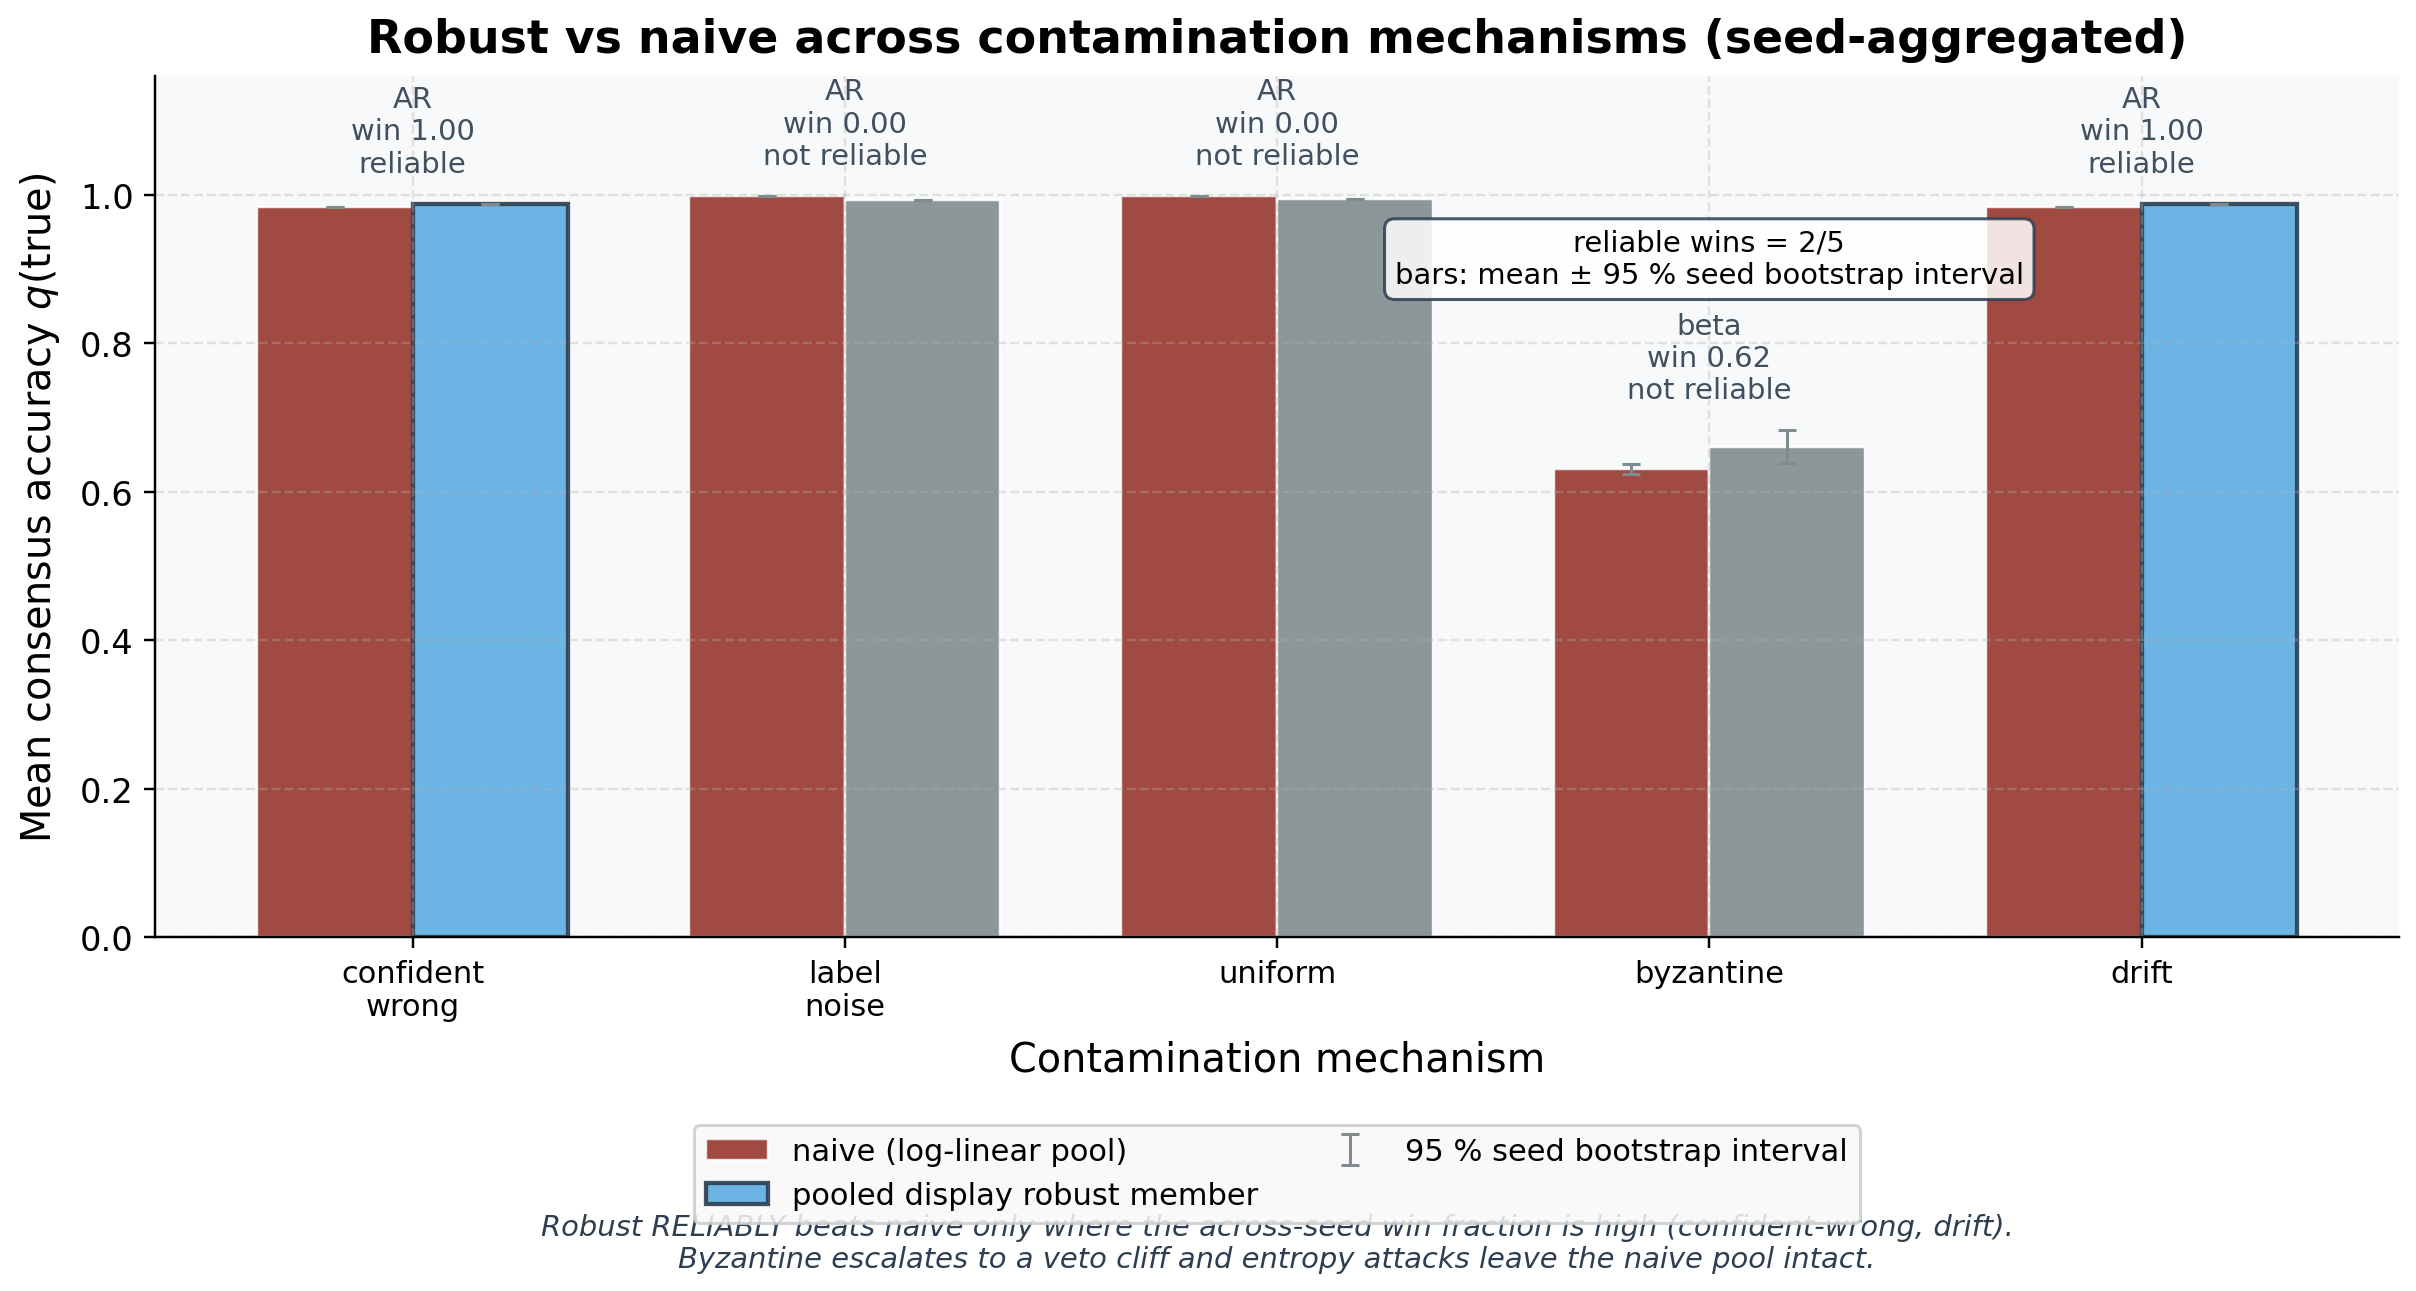
\includegraphics[width=0.85\linewidth,height=0.5\textheight,keepaspectratio,alt={Grouped bars compare naive pooling with the pooled display robust member for five contamination mechanisms. Bars show mean true-state consensus accuracy with seed-bootstrap intervals; annotations identify the selected method and its across-seed win fraction.}]{../figures/contamination_gallery.png}
\caption{Seed-aggregated mean consensus accuracy. Source relation:
original project contamination diagnostic; estimand: true-state accuracy
fraction by attack mechanism; uncertainty: the bars show 95\% seed-level
bootstrap confidence intervals for the pooled-selected display member,
while the adjacent table reports its conditional paired difference
interval. \(q(\text{true state})\) for the reference log-linear pool
versus the server preset selected once by pooled mean under each
contamination mechanism (\(n = 24\) trials \texorpdfstring{\ensuremath{\times}}{x} 64 seeds at strength 0.60).
The x-axis is the contamination mechanism; the y-axis is mean consensus
accuracy. Each group has two bars: an open, directly labeled
reference-log-pool bar and a hatched selected-server-preset bar whose
direct annotation names the preset and its across-seed win fraction. The
preset bar is drawn in full color only where that win fraction clears
the 0.95 display bar --- confident wrong, drift; the byzantine mechanism
and entropy attacks are muted because they do not clear that descriptive
screen. The in-figure summary gives the display-flag count across
mechanisms and reminds readers that the labels are win fractions, not
p-values. Bars are means over 64 independent configured seeds, with 24
matched trials nested within each seed. This is a descriptive
pooled-selection graphic, not selection-free post-selection inference;
the all-method review grid supplies the latter
surface.}\label{fig:contamination-gallery}
\end{figure}

\subsubsection{Robustness onset by corruption
mechanism}\label{sec:supp-onset}

The gallery fixes one contamination strength;
\breaktt{experiments.run\_robustness\_onset} maps the \emph{rate
dependence} (\(n = 24\) trials \texorpdfstring{\ensuremath{\times}}{x} 64 seeds per rate).

For each directional mechanism it reports the \textbf{descriptive onset
rate} --- the smallest rate at which the pooled-selected display
member's win fraction reaches 0.95 --- and that member's versus naive
accuracy at the worst (highest) swept rate. These display summaries are
not selection-free inference; the main-text all-method review grid in
sec.~\ref{sec:results-review-grid} is the inferential surface:

\begin{longtable}[]{@{}
  >{\raggedright\arraybackslash}p{(\linewidth - 8\tabcolsep) * \real{0.2000}}
  >{\raggedright\arraybackslash}p{(\linewidth - 8\tabcolsep) * \real{0.2000}}
  >{\raggedright\arraybackslash}p{(\linewidth - 8\tabcolsep) * \real{0.2000}}
  >{\raggedright\arraybackslash}p{(\linewidth - 8\tabcolsep) * \real{0.2000}}
  >{\raggedright\arraybackslash}p{(\linewidth - 8\tabcolsep) * \real{0.2000}}@{}}
\caption{Per-mechanism descriptive onset and worst-rate accuracy
(\(n = 24\) trials \texorpdfstring{\ensuremath{\times}}{x} 64 seeds). The onset rate is where the pooled
display method reaches the displayed win-fraction rule (win fraction \texorpdfstring{\textgreater{}=}{>=}
0.95); it is not a per-seed selection, selection-free inferential
result, or universal crossover
claim.}\label{tbl:robustness-onset}\tabularnewline
\toprule\noalign{}
\begin{minipage}[b]{\linewidth}\raggedright
Mechanism
\end{minipage} & \begin{minipage}[b]{\linewidth}\raggedright
Onset rate
\end{minipage} & \begin{minipage}[b]{\linewidth}\raggedright
Naive @ worst
\end{minipage} & \begin{minipage}[b]{\linewidth}\raggedright
Robust @ worst
\end{minipage} & \begin{minipage}[b]{\linewidth}\raggedright
Robust method @ worst
\end{minipage} \\
\midrule\noalign{}
\endfirsthead
\toprule\noalign{}
\begin{minipage}[b]{\linewidth}\raggedright
Mechanism
\end{minipage} & \begin{minipage}[b]{\linewidth}\raggedright
Onset rate
\end{minipage} & \begin{minipage}[b]{\linewidth}\raggedright
Naive @ worst
\end{minipage} & \begin{minipage}[b]{\linewidth}\raggedright
Robust @ worst
\end{minipage} & \begin{minipage}[b]{\linewidth}\raggedright
Robust method @ worst
\end{minipage} \\
\midrule\noalign{}
\endhead
\bottomrule\noalign{}
\endlastfoot
byzantine & 0.4 & 0.0165 & 0.0000 & beta \\
confident wrong & 0.6 & 0.6676 & 0.7772 & beta \\
drift & 0.6 & 0.6676 & 0.7772 & beta \\
\end{longtable}

The mechanism-specific onset thresholds are collected in
tbl.~\ref{tbl:robustness-onset}.

The rate dependence sharpens the gallery's snapshot, and
fig.~\ref{fig:robustness-onset} draws it. The additive confident-wrong
and drift attacks degrade the naive pool gradually; past their onset
rate the robust member stays above it through to the worst rate.

The multiplicative byzantine attack is qualitatively different: it opens
an \emph{early} robustness window --- robust overtakes at a lower onset
rate --- but then escalates to the veto cliff where naive and robust
both collapse, so its worst-rate accuracy is near zero for both.

This is the rate-resolved bounded interpretation: the displayed contrast
is sustained against the two additive directional mechanisms and only
transient against the multiplicative mechanism.

\begin{figure}
\centering
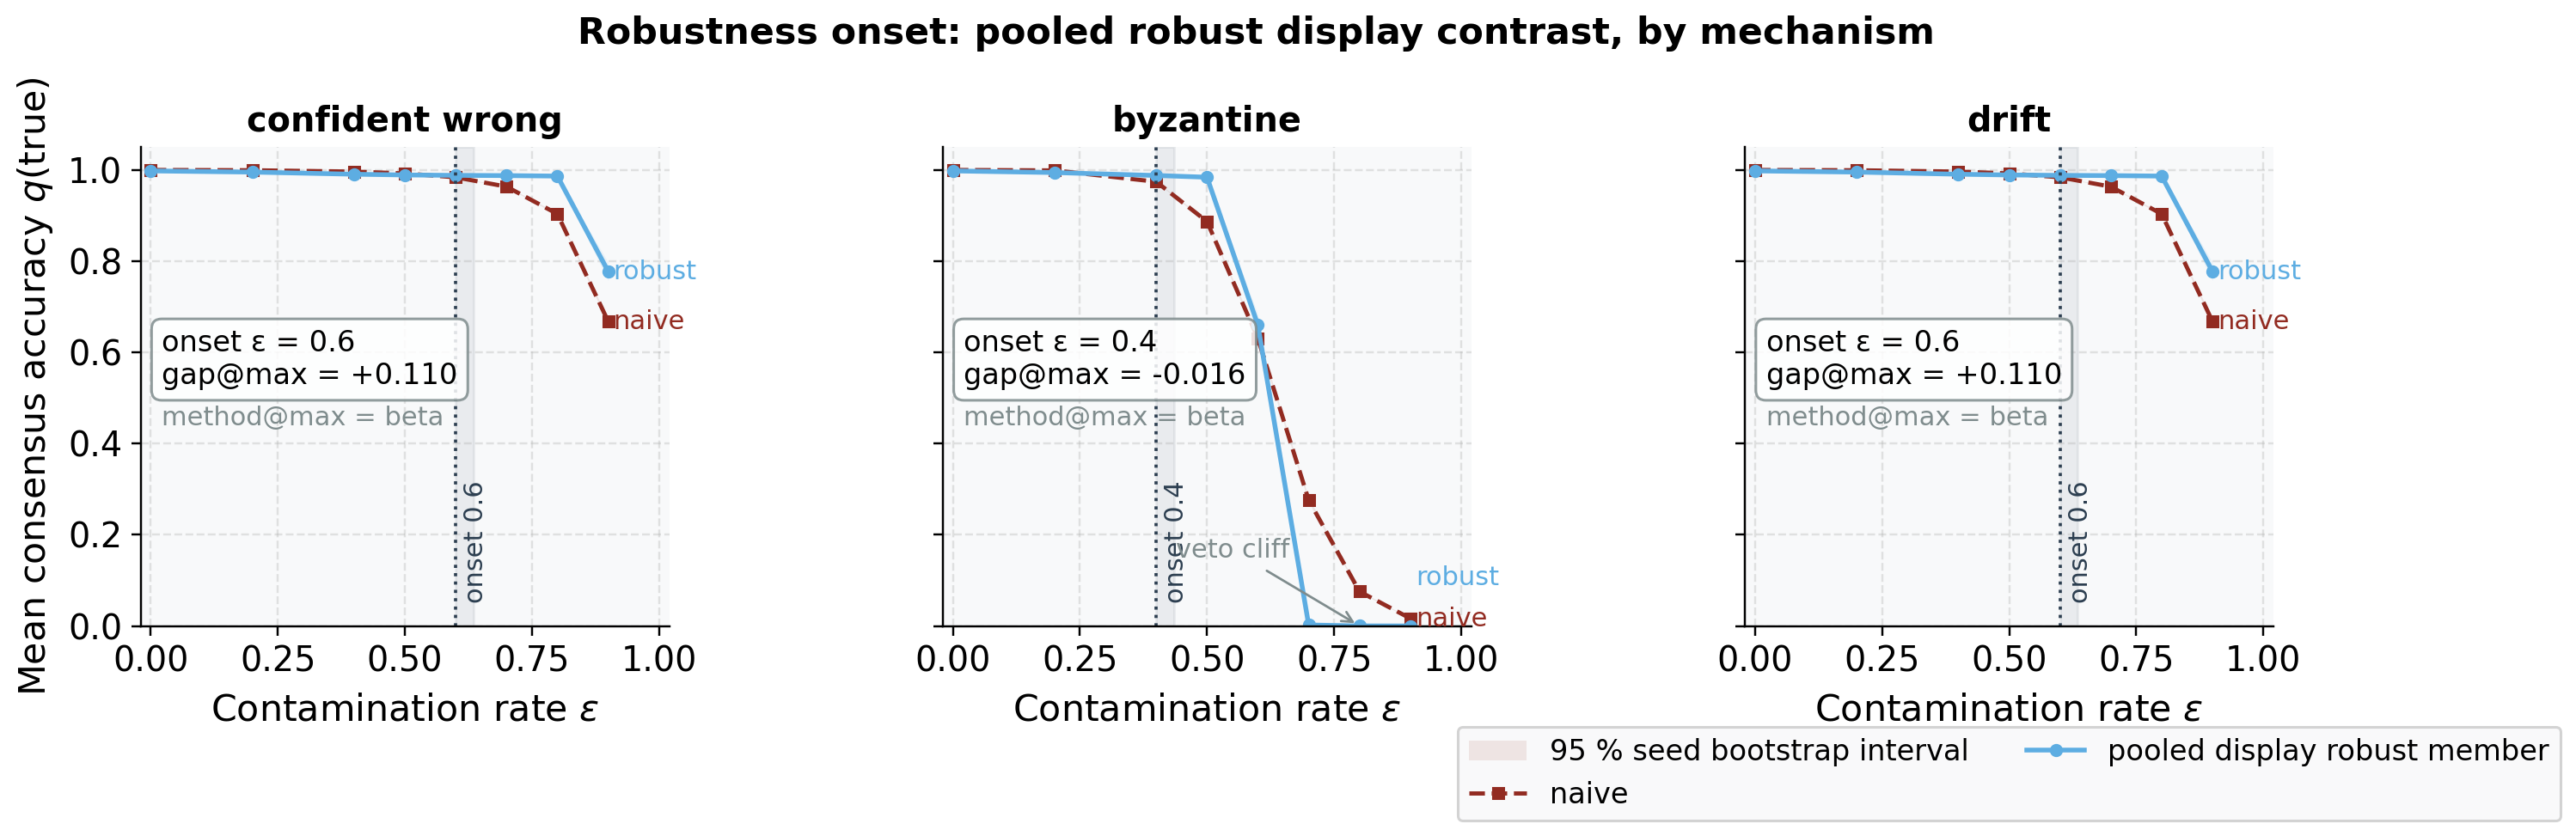
\includegraphics[width=0.95\linewidth,height=0.5\textheight,keepaspectratio,alt={Three mechanism-specific panels plot pooled robust-member and naive consensus accuracy against contamination rate. Vertical lines mark descriptive onset rates, and byzantine contamination shows a transient contrast before collapse.}]{../figures/robustness_onset.png}
\caption{Reference log pool and pooled-selected server preset across
attack rates. Source relation: original project robustness-onset
diagnostic; estimand: mean consensus accuracy fraction by attack rate;
uncertainty: shaded 95\% percentile-bootstrap intervals over configured
seeds, conditional on the pooled-selected display member. Each panel
reads left to right as contamination increases: filled circles with a
solid line identify the reference log pool, while open squares with a
dashed line identify the pooled display server preset selected once by
pooled mean across seeds at each rate. The x-axis is contamination rate
and the y-axis is mean consensus accuracy. Each of 64 independent
configured seeds contains 24 nested trials per rate; trials are not
promoted to independent replicates. A dark dotted vertical rule marks
the descriptive onset rate (pooled preset win fraction \texorpdfstring{\textgreater{}=}{>=} 0.95), and the
inset reports that onset plus the terminal preset-minus-reference gap.
Confident-wrong and drift retain a displayed contrast after onset;
Byzantine contamination produces a transient window before both methods
lose consensus accuracy at the largest rates. The companion table gives
the displayed onset, terminal values, and selected preset. This
pooled-selection figure is descriptive, not selection-free
post-selection inference; the all-method review grid supplies the
selection-free comparative surface.}\label{fig:robustness-onset}
\end{figure}

\subsubsection{Conditional world and attack-geometry
grid}\label{sec:supp-conditional-world}

The finite MAJ-1 characterization is now extended across 40
preregistered world/scenario cells: two hidden-state locations, two
observability levels, five attack mechanisms, and two adversarial weight
settings.

The independent unit is the seeded world/scenario row; each cell
averages 24 nested trials over 64 seeds before the matched contrast is
formed. The primary estimand is naive true-state error minus robust
true-state error, so a positive value means the robust heuristic assigns
more true-state mass in that finite cell.

The robustness-zero control is pass, and the report remains explicitly
labelled \breaktt{conditional\_finite\_grid}. The resulting conditional
surface is shown in fig.~\ref{fig:conditional-world}.

\begin{figure}
\centering
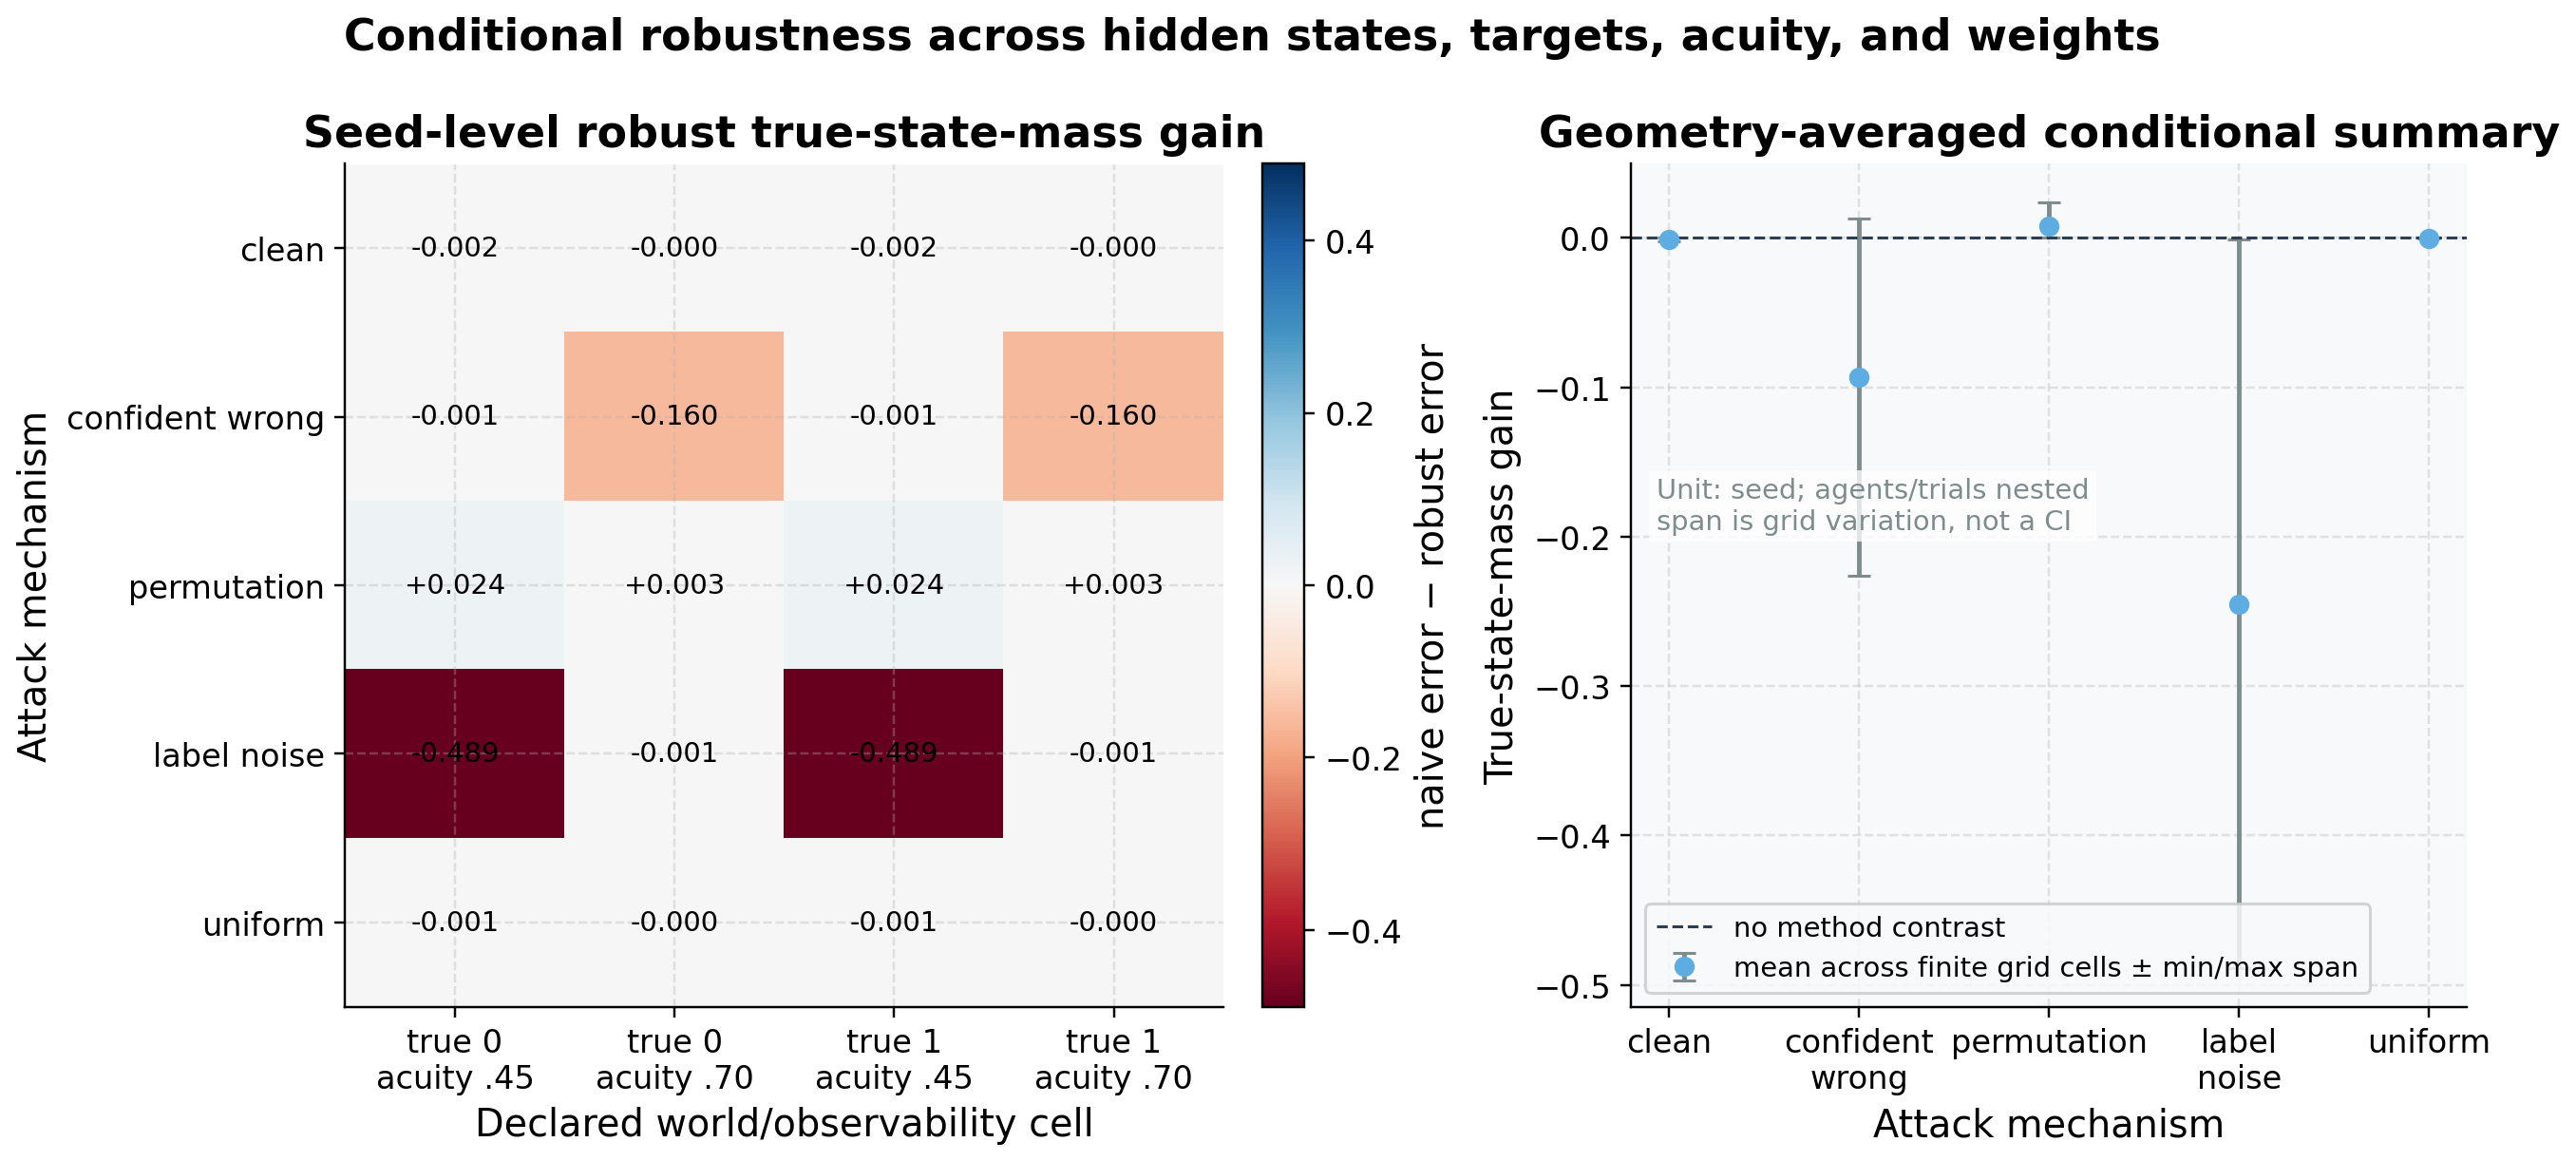
\includegraphics[width=0.95\linewidth,height=0.5\textheight,keepaspectratio,alt={Two-panel finite-grid robustness diagnostic. The left heatmap shows the robust-minus-naive true-state-mass contrast across attack mechanisms and world or acuity cells; the right panel shows finite-grid means with min/max spans by attack mechanism.}]{../figures/conditional_world.png}
\caption{Conditional-world robustness grid. Source relation: original
project finite-grid generalization of the MAJ-1 characterization;
estimand: naive true-state error minus robust true-state error in
probability-mass units. In Panel A, the x-axis indexes hidden-state and
observability cells and the y-axis indexes attack mechanisms; every
heatmap cell prints its signed seed-level mean, so sign and magnitude
remain available without colour. The source report retains a 95\%
seed-bootstrap interval for each cell. In Panel B, the x-axis is the
signed contrast and the y-axis again lists attacks. Its point is the
mean over all declared finite-grid cells for that attack, and the
asymmetric capped whiskers extend to the observed cell minimum and
maximum. These capped min/max spans are finite-grid ranges, not
confidence intervals and not symmetric mean-plus-or-minus errors. A
dark-neutral dotted zero rule marks no method contrast. Positive values
favour robust true-state mass; negative values favour naive pooling. The
independent unit is the seeded world/scenario row, with 24 trials nested
within each row. This is conditional evidence over a declared finite
grid, not a theorem, breakdown bound, universal attack result, or
estimate of performance beyond the registered
worlds.}\label{fig:conditional-world}
\end{figure}

\subsubsection{Proper scores and calibration
controls}\label{sec:supp-belief-quality}

Argmax accuracy does not distinguish a cautious posterior from an
overconfident one. The scoring extension therefore pre-registers the
paired seed-level categorical log-score difference between naive and
robust consensus beliefs as its primary belief-quality estimand. The
Brier score and equal-width expected calibration error are secondary
diagnostics; higher log score and lower Brier/ECE are better. Agents and
trials remain nested within the seed.

The report also includes three negative controls: an oracle, a uniform
belief, and a confidently wrong belief. Their expected score ordering is
checked before any method contrast is interpreted: oracle \textgreater{}
uniform \textgreater{} confidently wrong under the clipped log score.
The control ordering gate is \texttt{pass}, and the
confidently-wrong-versus-uniform control is \texttt{pass}, using 64
independent seeds and 24 nested trials per seed. The diagnostic is shown
in fig.~\ref{fig:belief-quality}.

\begin{figure}
\centering
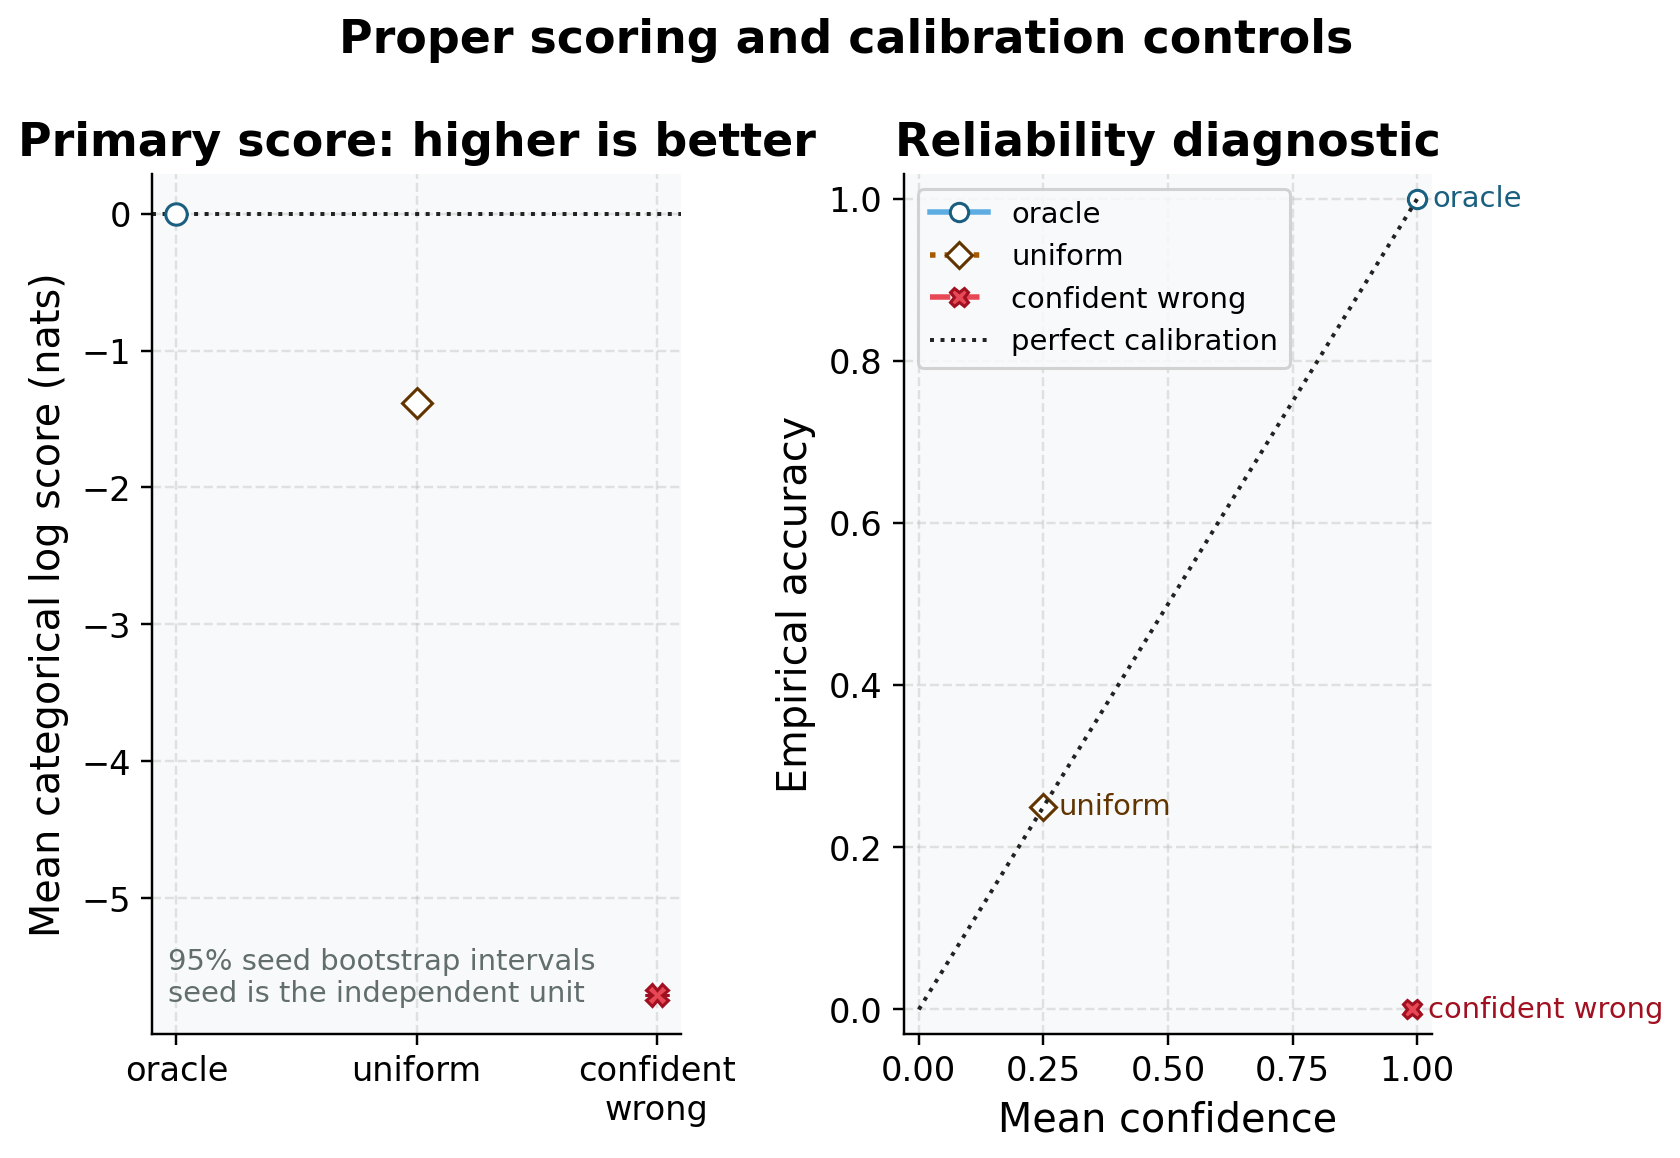
\includegraphics[width=0.9\linewidth,height=0.5\textheight,keepaspectratio,alt={Two-panel control figure. Open circles, open diamonds, and filled crosses compare oracle, uniform, and confidently-wrong categorical log scores with seed intervals; the right panel uses the same marker-and-dash identities for binned reliability coordinates against a dotted perfect-calibration line. Brier score and ECE remain report-only diagnostics.}]{../figures/belief_quality.png}
\caption{Proper-score and reliability controls. Source relation:
original project belief-quality diagnostic; displayed estimands:
categorical log score in nats and binned mean-confidence versus
empirical-accuracy coordinates in fractions. The x-axis is control type
in Panel A and mean confidence in Panel B; the y-axis is mean
categorical log score and empirical accuracy, respectively. Open circles
identify oracle controls, open diamonds identify uniform controls, and
filled crosses identify confidently-wrong controls; the reliability
panel retains the same marker-and-dash identities, direct endpoint
labels, and a dark dotted perfect-calibration rule. Panel A's capped
whiskers are 95\% percentile-bootstrap intervals across independent
configured seeds. Trials are nested within seed, and the reliability
coordinates display no separate interval. Brier score and expected
calibration error are retained as report-only secondary diagnostics and
are not plotted in this two-panel figure. The ordered controls test
score and reliability implementation on the configured finite world;
they do not establish decision optimality, calibration under
distribution shift, or robustness beyond the tested
conditions.}\label{fig:belief-quality}
\end{figure}

\subsection{Greedy multi-hypothesis model reduction beyond the main BMR
study}\label{sec:supp-greedy-bmr}

The single-step reduction of sec.~\ref{sec:method-learning} scores one
candidate reduced prior. \breaktt{bayesian\_model\_reduction.py} adds
\texttt{greedy\_reduce}, which performs structure learning over a
\emph{family} of redundant states: starting from the full prior, it
scores pruning each not-yet-pruned state against the current reduced
prior, accepts the single prune with the largest positive free-energy
gain, and repeats until no remaining prune improves model evidence.

Every accepted step has a strictly positive incremental \(\Delta F\), so
the cumulative evidence is monotone-increasing and the search recovers
the sparse generative model the data support --- a state with genuine
evidence yields \(\Delta F < 0\) when pruned and is kept.

This is the multi-state analogue of the configured BMR sign-control
result of sec.~\ref{sec:results-emergence}, and is verified directly in
the model-reduction tests.

\subsection{Federation transport protocol and bit-identity
witness}\label{sec:supp-federation}

\ifcsname proposition\endcsname
\else
\newtheorem{proposition}{Proposition}
\fi

This supplement answers a concrete question the main text raises but
settles elsewhere: when belief sharing is routed through an actual
transport channel instead of a direct function call, does the fused
consensus change? It specifies that transport --- the same single-host
interface sec.~\ref{sec:future-transport} names as the anchor for
eventual multi-machine federation --- and establishes that, under a
lossless round-trip, the answer is no.

Concretely, the transport realizes belief sharing over a real in-memory
channel rather than a direct aggregation call. Each worker holds a local
posterior \(q_n\) over the shared latent factor and serializes it to
lossless IEEE-754 float64 bytes using the numpy-lossless-float64
encoding (numpy's native array format), guaranteeing bit-identical
round-trip across the transport boundary.

A server collects 5 such beliefs, fuses them with the same robust server
step at robustness \(c = 1.5\), and broadcasts the consensus \(q\) back
to every contributing worker over its response channel.

\begin{proposition}[Federation bit-identity]\label{prop:federation-bit-identity}
When the transport serialization is lossless — an exact IEEE-754 float64
round-trip — the federated consensus equals the in-process aggregation
\(q = \mathrm{robust\_aggregate}(\{q_n\}, c)\) bit-for-bit. Transport moves
bytes, not mathematics, so no precision is lost and no result changes.
\end{proposition}

Because the round-trip is exact, this implementation retires the direct
in-process serialization caveat. The queue adapter remains a genuine
\texttt{queue.Queue} transport, \breaktt{run\_multiprocess\_round}
exercises the same server/worker protocol with one OS worker process per
agent on a single machine, and \breaktt{run\_socket\_round} exercises the
loopback-TCP adapter. The fused result is provably unchanged.
Bit-identity verified: True.

The implementation lives in the \texttt{federation/} package. The
end-to-end and socket transport tests exercise the full round-trip ---
worker serialization, server aggregation, consensus broadcast,
out-of-order arrival, the single-machine process helper, loopback TCP
framing, optional HMAC frame integrity, and file-backed digest-verified
replay validation --- and assert bit-identity against the in-process
\breaktt{robust\_aggregate} result.

A caller-owned SQLite guard rejects reused round IDs across local
process restarts, but does not define a shared multi-host replay domain.

This test surface is the API contract that
sec.~\ref{sec:future-transport} identifies as the anchor for future
network transport: the aggregation mathematics can remain unchanged, but
true multi-machine work still requires cross-host transport,
identity-bound mTLS, shared replay state, discovery, restart
orchestration, and threat-model validation that this single-host
evidence does not supply.

\section{Supplemental notation contract}\label{sec:supp-notation}

This supplement is the authoritative notation contract for Active
Fedference. The methods, formalism, results, figures, report schemas,
and API documentation use these meanings even when a source paper uses a
different symbol. A symbol is not reused for a different mathematical
object merely because the objects are both probability vectors.

The implementation names in the final column are the canonical names for
new code and reports; old names survive only as warned, parity-tested
compatibility adapters.

\subsection{Probability objects and generative-model
quantities}\label{probability-objects-and-generative-model-quantities}

\subsubsection{States, posteriors, and site
factors}\label{states-posteriors-and-site-factors}

{\def\LTcaptype{none} % do not increment counter
\begin{longtable}[]{@{}ll@{}}
\toprule\noalign{}
Symbol & Meaning \\
\midrule\noalign{}
\endhead
\bottomrule\noalign{}
\endlastfoot
\(s\) & Hidden categorical-state index. \\
\(o\) & Observation/outcome index. \\
\(q_n(s)\) & Agent \(n\)'s updated local posterior. \\
\(q(s)\) & Server consensus posterior. \\
\(q_{-n}(s)\) & Normalized cavity excluding site \(n\). \\
\(t_n(s)\) & Agent \(n\)'s natural-parameter site. \\
\(m_n(s)\) & Bridge-only source log potential. \\
\end{longtable}
}

Here \(s\in\{1,\ldots,n_s\}\) and \(o\in\{1,\ldots,n_o\}\) are indices,
not distributions. Each \(q_n(s)\) is the local posterior over the
shared latent state after agent \(n\)'s update; \(q(s)\) is the
corresponding server consensus, and \(q_{-n}(s)\) removes agent \(n\)'s
site contribution. The site \(t_n(s)\) is a natural-parameter factor.
The bridge-only quantity satisfies \(m_n(s)=\log q_n(s)+\kappa_n\) for
state-constant \(\kappa_n\); it has no project API and does not imply
that every source-protocol message is a broadcast posterior.

The corresponding code terms are \texttt{state}, \texttt{observation},
\texttt{local\_posteriors{[}n{]}}, \breaktt{global\_posterior} or
\texttt{consensus}, \texttt{cavity(...)}, and \texttt{site\_factor}, in
table order through \(t_n(s)\). The bridge-only \(m_n(s)\) has no
project API.

\subsubsection{Priors, policies, and POMDP
quantities}\label{priors-policies-and-pomdp-quantities}

{\def\LTcaptype{none} % do not increment counter
\begin{longtable}[]{@{}ll@{}}
\toprule\noalign{}
Symbol & Meaning \\
\midrule\noalign{}
\endhead
\bottomrule\noalign{}
\endlastfoot
\(\pi_0(s)\) & Hidden-state prior, not a policy. \\
\(\boldsymbol{\pi}\) & Policy or action sequence. \\
\(A[o,s]=P(o\mid s)\) & Observation-likelihood matrix. \\
\(B[s',s,u]=P(s'\mid s,u)\) & State-transition tensor. \\
\(C[o]\) & Outcome log-preference. \\
\(D_0[s]\) & Initial POMDP state prior. \\
\(q(o\mid\boldsymbol{\pi})\) & Policy-conditional predicted outcomes. \\
\end{longtable}
}

The state index \(s\), posterior \(q(s)\), prior \(\pi_0(s)\), and
policy \(\boldsymbol{\pi}\) must not be conflated. In particular, the
policy symbol is bold when needed, never used for a prior, and the prior
is never called a policy. The uppercase POMDP tensors \(A,B,C,D_0\) are
model objects; they are not posterior factors. Each state-indexed column
of \(A\) is a pmf. The tensor \(B\) is indexed by next state, current
state, and control. The preferred-outcome pmf is
\(p_C(o)=\operatorname{softmax}(C)[o]\), and
\(q(o\mid\boldsymbol{\pi})\) is the predicted-outcome distribution used
in EFE calculations.

The canonical code terms, in table order, are \texttt{prior} or
\texttt{log\_prior}, \texttt{policy}, \texttt{likelihood},
\texttt{transition}, \texttt{log\_preferences}, \texttt{initial\_prior},
and \breaktt{predicted\_outcomes}.

For the qualified relation to Friston et al.'s Eq. 7
\citep{friston2024federated}, the shared support is finite, every
\(q_n(s)\) is positive on it, the Eq. 7 softmax input is represented by
the bridge-only \(m_n(s)\) above, and the declared weights \(w_n\) are
fixed rather than functions of the emerging consensus.

Under exactly those assumptions, additive \(\kappa_n\) constants cancel
under softmax and eq.~\ref{eq:log-linear-pool} is the categorical
posterior-log-potential specialization of the source message-combination
term. It neither reconstructs source message construction,
cavity/exclusion policy, scheduling, generative factors, nor the
complete source protocol.

\subsection{Divergences, losses, and scalar
controls}\label{divergences-losses-and-scalar-controls}

\subsubsection{Generalized-Bayes and aggregation
terms}\label{generalized-bayes-and-aggregation-terms}

{\def\LTcaptype{none} % do not increment counter
\begin{longtable}[]{@{}ll@{}}
\toprule\noalign{}
Symbol & Meaning \\
\midrule\noalign{}
\endhead
\bottomrule\noalign{}
\endlastfoot
\(\mathcal D(q\Vert p)\) & Regularizing divergence. \\
\(L(s;o)\) & Statewise loss for observation \(o\). \\
\(\tau>0\) & Generalized-Bayes learning rate. \\
\(w_n\) & Supplied non-negative base weight. \\
\(a_n\) & Raw variational effective weight. \\
\(\widetilde a_n=a_n/\sum_m a_m\) & Normalized influence weight. \\
\end{longtable}
}

The regularizing divergence acts between distributions and may be KL,
reverse KL, or \(\alpha\)-Rényi. The positive learning rate/temperature
\(\tau\) multiplies accumulated loss and accepts \texttt{learning\_rate}
only as a warned compatibility alias.

The symbols \(w_n\), \(a_n\), and \(\widetilde a_n\) are deliberately
distinct. The first is supplied before aggregation, the second is the
variational raw server output satisfying \(0\le a_n\le w_n\), and the
third is only its normalized influence representation returned for
interpretation and plotting.

Their canonical code terms, in table order, are \texttt{divergence},
\texttt{loss\_by\_state}, \texttt{tau}, \texttt{base\_weights{[}n{]}},
\texttt{raw\_effective\_weights{[}n{]}}, and
\texttt{normalized\_effective\_weights{[}n{]}}.

The server heuristic's reweighting is not a FedGVI client loss and does
not inherit a client-side robustness theorem. \breaktt{robust\_aggregate}
is a server heuristic with the tested \(c=0\) recovery identity.
\breaktt{variational\_aggregate} owns the explicit finite-simplex
objective and the raw-weight bound; that bound is not an estimator-level
B-robustness theorem.

\subsubsection{Robustness, divergences, and loss
controls}\label{robustness-divergences-and-loss-controls}

{\def\LTcaptype{none} % do not increment counter
\begin{longtable}[]{@{}ll@{}}
\toprule\noalign{}
Symbol & Meaning \\
\midrule\noalign{}
\endhead
\bottomrule\noalign{}
\endlastfoot
\(c\ge0\) & Server divergence-reweighting coefficient. \\
\(\lambda>0\) & Variational-objective entropy weight. \\
\(\alpha>0\) & Rényi-divergence order. \\
\(\beta\ge0\) & Density-power-loss parameter. \\
\(q_{\text{loss}}>0\) & Robust categorical-cross-entropy parameter. \\
\(\rho\in[0,1]\) & Declared contamination rate. \\
\end{longtable}
}

The coefficient \(\lambda\) controls the variational objective and its
coordinate updates; \(\lambda\downarrow0\) is a separate deterministic
tied-argmax endpoint. The parameter \(q_{\text{loss}}\) belongs to
\(L_{q_{\text{loss}}}\); its \(q_{\text{loss}}\downarrow0\) NLL limit is
handled separately, and the subscript prevents collision with posterior
\(q(s)\). Contamination rate \(\rho\) is always interpreted within the
declared attack mechanism.

The associated code terms are \texttt{robustness},
\texttt{entropy\_weight}, \texttt{alpha}, \texttt{beta},
\texttt{q\_loss}, and \breaktt{contamination\_rate} or \texttt{rate}, in
table order.

For the objective-backed server rule, the complete scalar-control
contract is defined for \(c>0\) and \(\lambda>0\):

\begin{equation}\protect\phantomsection\label{eq:notation-variational-objective}{
\begin{aligned}
F_\lambda(q,a)
 &= \sum_n a_n\,\mathrm{CE}(q,q_n)
    -\lambda H(q)\\
 &\qquad +\frac{1}{c}\,\mathrm{KL}_{\rm gen}(a\Vert w).
\end{aligned}
}\end{equation}

Its two coordinate updates are shown separately so each display remains
legible at the presentation typography floor:

\begin{equation}\protect\phantomsection\label{eq:notation-variational-updates}{
\begin{aligned}
q &\propto \exp\!\left(
\frac{1}{\lambda}\sum_n a_n\log q_n\right),\\
a_n &= w_n\exp\!\big[-c\,\mathrm{CE}(q,q_n)\big].
\end{aligned}
}\end{equation}

The coordinate updates eq.~\ref{eq:notation-variational-updates} use
\(\lambda=1.0\) by default; the \texttt{entropy\_weight} argument
exposes the stated tempered family. The \(c=0\) branch is handled as a
recovery limit outside the \(c>0\) objective; at \(\lambda=1.0\) it is
the exact project log-linear pool. The \(\lambda\downarrow0\) endpoint
is separately implemented as a deterministic tied-argmax rule and is not
obtained by substituting \(\lambda=0\) into the displayed objective or
update.

\subsection{Cavity and factor algebra}\label{cavity-and-factor-algebra}

For a positive-support global posterior and site term, the cavity
operation is defined in log space and then normalized:

\begin{equation}\protect\phantomsection\label{eq:notation-cavity}{
\begin{aligned}
q_{-n}(s)
&= \frac{q(s)/t_n(s)}{\sum_{s'}q(s')/t_n(s')}\\
&= \operatorname{softmax}\!\left(\log q(s)-\log t_n(s)\right).
\end{aligned}
}\end{equation}

The corresponding factor replacement is

\begin{equation}\protect\phantomsection\label{eq:notation-factor-replacement}{
\begin{aligned}
\ell_n(s)
&= \log t_n^{\mathrm{old}}(s)\\
&\quad +\log q^{\mathrm{new}}(s)-\log q^{\mathrm{old}}(s),\\
t_n^{\mathrm{new}}(s)
&\leftarrow \operatorname{softmax}(\ell_n)(s).
\end{aligned}
}\end{equation}

Here \(\ell_n\) is the transient, unnormalized log-site vector; the
softmax is exactly the exponential normalization of that vector.

The code-level \texttt{cavity} adapter takes \breaktt{global\_posterior}
and \texttt{site\_factor}. The \texttt{update\_factor} adapter takes
\texttt{old\_site\_factor}, \breaktt{old\_global\_posterior}, and
\breaktt{new\_global\_posterior}. The old keywords \texttt{posterior},
\texttt{factor}, \texttt{old\_factor}, \texttt{old\_posterior}, and
\texttt{new\_posterior} are accepted only with a
\breaktt{DeprecationWarning}; mixed canonical/old calls fail closed.

Recombination is tested by normalizing \(q_{-n}(s)t_n(s)\) and checking
recovery of \(q(s)\) to floating-point tolerance. A transported site
factor is represented as a pmf, so its arbitrary positive
natural-parameter scale is fixed by the explicit normalization above.

\subsection{Statistical notation and
nesting}\label{statistical-notation-and-nesting}

{\def\LTcaptype{none} % do not increment counter
\begin{longtable}[]{@{}
  >{\raggedright\arraybackslash}p{(\linewidth - 2\tabcolsep) * \real{0.5000}}
  >{\raggedright\arraybackslash}p{(\linewidth - 2\tabcolsep) * \real{0.5000}}@{}}
\toprule\noalign{}
\begin{minipage}[b]{\linewidth}\raggedright
Symbol
\end{minipage} & \begin{minipage}[b]{\linewidth}\raggedright
Contractual meaning
\end{minipage} \\
\midrule\noalign{}
\endhead
\bottomrule\noalign{}
\endlastfoot
\(n_{\rm seed}\) & Number of independently seeded worlds/replicates in a
declared cell; the inferential unit for seed-level summaries. \\
\(n_{\rm trial}\) & Number of trials nested within one seed and cell;
trials are averaged before seed-level inference. \\
\(\Delta=b-a\) & Matched robust-minus-naive contrast for the same
seed/trial or the declared seed-level reduction. \\
\(r_{\rm rb}\) & Wilcoxon matched-pairs rank-biserial effect, primary
standardized effect. \\
\(d_{\rm eq}\) & \(2r_{\rm rb}/\sqrt{1-r_{\rm rb}^2}\), a secondary
rank-biserial-derived display/planning d-equivalent, not raw Cohen's
\(d\). \\
\(\mathrm{CI}_{1-\alpha}\) & Percentile bootstrap interval for the named
estimand, resampling the declared replication unit. \\
\(\mathrm{MCSE}\) & Monte Carlo standard error/precision diagnostic for
a simulation summary; it is not a confidence interval. \\
\(\mathrm{MDE}\) & Observed-design minimum detectable effect diagnostic
under its stated approximation; it is not confirmatory evidence. \\
\(p,q\) & Raw p-value and BH-adjusted q-value; the family and ownership
are declared with every report. \\
\end{longtable}
}

For the robustness sweep, the primary result is \(r_{\rm rb}\) and the
matched mean difference \(\overline{\Delta}\) with its bootstrap
interval. The d-equivalent is retained only as a monotone secondary
display and planning input. When \(|r_{\rm rb}|=1\), the transform
diverges; reports use a finite sentinel and captions disclose saturation
rather than presenting a million-scale number as a scientifically
interpretable effect.

Power, prospective sample size, MCSE, and MDE are observed-effect
planning/precision diagnostics, not evidence that a confirmatory effect
exists.

The predeclared headline display rule is the largest positive
\(r_{\rm rb}\) among robust methods, with the declared method order as a
deterministic tie break. A report must also expose the complete
tied-method set, the tie-break, the method with the largest mean
\(\overline{\Delta}\), and the method with the largest mean at the worst
rate.

These are distinct summaries; none is a unique scientific winner when
the evidence is tied or conditional.

For the review grid, every configured robust method remains an
inferential member and a displayed rate-profile curve. No pooled-mean
selection creates a curve, interval, or hypothesis-test member for that
surface.

\subsection{Code and manuscript naming
map}\label{code-and-manuscript-naming-map}

Every arrow names a legacy surface followed by its canonical
replacement.

\textbf{Belief inputs.} \texttt{beliefs} or \texttt{agent\_beliefs} \texorpdfstring{\ensuremath{\to}}{->}
\breaktt{local\_posteriors}; \texttt{weights} \texorpdfstring{\ensuremath{\to}}{->} \texttt{base\_weights}.
Both are warned keyword/property adapters.

\textbf{Aggregation outputs.} Result property \texttt{agent\_weights} \texorpdfstring{\ensuremath{\to}}{->}
\breaktt{normalized\_effective\_weights}; variational argument
\texttt{agent\_weights} \texorpdfstring{\ensuremath{\to}}{->} \breaktt{raw\_effective\_weights}. Both are
warned adapters, but represent different weight scales.

\textbf{Diagnostics.} \texttt{shared\_beliefs} \texorpdfstring{\ensuremath{\to}}{->}
\breaktt{shared\_posteriors}; \texttt{loss\_vec} \texorpdfstring{\ensuremath{\to}}{->}
\texttt{loss\_by\_state}. These are warned diagnostics and keyword
adapters.

\textbf{Statistics.} \breaktt{cohens\_d\_from\_rank\_biserial} \texorpdfstring{\ensuremath{\to}}{->}
\breaktt{d\_equivalent\_from\_rank\_biserial}; report field
\texttt{cohens\_d} \texorpdfstring{\ensuremath{\to}}{->} \texttt{d\_equivalent}. The function is a warned
adapter; the report change is a versioned migration.

These adapters never silently reinterpret an argument or result. The
\texttt{agent\_weights} result property preserves serialized wire
compatibility, while the variational objective and new reports use the
canonical weight terms. New reports are canonical and schema-versioned;
readers fail closed on unsupported versions.
\breaktt{d\_equivalent\_from\_rank\_biserial} returns the declared
rank-biserial-derived d-equivalent, not raw Cohen's \(d\);
\texttt{loss\_vec} remains only a warned generalized-Bayes keyword
adapter.

The wire-level key \texttt{agent\_weights} is preserved because it is a
federation transport contract, not a claim about the scale or meaning of
the new result fields. A future wire migration requires an explicit
version and a fail-closed reader; it must not silently reinterpret the
key.

\subsection{Source and evidence
boundaries}\label{source-and-evidence-boundaries}

The Friston belief-sharing equations are source equations/protocol
claims. Only under the explicit finite-shared-support,
posterior-log-potential, and fixed-weight bridge above does the
categorical log-linear pool specialize the source message-combination
term; the tested \(c=0\) identity remains project-local. The
generalized-Bayes and loss limits are implementation analogues checked
in the finite categorical model.

The contamination, gallery, onset, conditional-world, and review-grid
quantities are conditional simulation evidence over declared cells. None
of these finite surfaces is an external-data replication, a
reconstructed source protocol, a universal attack taxonomy, a causal
intervention, or a proof of a server-side robustness guarantee.

Open theory, calibration, protocol, continuous-state, external-data,
authenticated-federation, and clean-release work remains open in the
project TODO and claim-audit documents.

\subsection{Moving sentinel world: communication contrast depends on
field of view}\label{sec:results-moving}

The hidden-state/action relation for this extension is summarized in the
categorical loop schematic fig.~\ref{fig:pomdp-loop}; the results below
remain the executed moving-world comparisons, not a claim that the
schematic's full loop is present in every flat belief-sharing study.

The static sentinel world lets every agent observe the same shared
latent, so belief sharing is a refinement rather than a requirement. To
stress the \emph{necessity} of communication we add movement and
\textbf{disjoint} fields of view.

The world is a linear grid of 4 cells holding a single binary threat ---
left half (state 0) or right half (state 1). The 2 sentinels start at
evenly tiled positions and each observe a half-open window of cells, so
in the default setup agent 0 watches the left half and agent 1 the right
half: their views do not overlap.

Each agent's likelihood is a confident, signed presence reading for the
half it can see, and three control paths (stay / left / right) let it
reposition. The expected-free-energy policy scores each candidate move
by the expected posterior entropy after one observation and takes the
most information-seeking step.

We run 960 trials of 6 steps each under three conditions:
\emph{isolated} (random moves, no sharing), \emph{communicating} (random
moves plus a log-linear-pool consensus each step), and \emph{EFE-guided}
(information-seeking moves plus the same sharing).

The measured consensus accuracies are 0.999 (isolated), 0.977
(communicating), and 0.978 (EFE-guided), with a communicating
free-energy gap of -0.528 nats relative to the isolated baseline
(negative: no free-energy advantage over isolated in this
binary-complement regime of logically complete half-views)
(fig.~\ref{fig:moving-world}).

Across 128 independent seeds the EFE-guided accuracy is 0.983 (95 \% CI
0.982--0.984), the communicating (random-moves + sharing) accuracy is
0.982 (95 \% CI 0.982--0.983), and the isolated accuracy is 0.999 (95 \%
CI 0.999--0.999).

In this binary-complement regime the isolated condition is in fact
significantly \emph{higher} on accuracy than the EFE-guided sharing
condition --- their 95 \% intervals do not overlap --- and the
EFE-vs-isolated accuracy contrast yields Wilcoxon signed-rank
\(p = 9.27 \times 10^{-23}\) (significant; isolated higher), effect size
\(r = 1.000\) (large). Sharing is therefore not merely unnecessary in
this regime; it costs a small but reliable amount of accuracy.

Nor does sharing lower free energy here: the EFE free-energy gap
(isolated surprise minus the EFE-guided condition's surprise) is -0.368
nats (95 \% CI -0.384---0.353) --- negative, so the pooled consensus is
slightly \emph{more} surprised by the true state than the isolated
baseline, because a single agent's view already suffices.

The accuracy case for \emph{necessity} is therefore made only in the
larger-state-space disjoint-FOV extension below, not by these
binary-complement numbers.

We report these numbers as measured, not assumed. The binary world
carries a logical complement: ruling out one's own half implies the
other, so a single agent's ``not detected'' still carries information
about the global state, and an isolated agent is not strictly blind.

By design, the intended \emph{cannot-decide-alone} regime is the
high-noise, few-step corner where one sensor's evidence cannot overcome
the flat prior; there belief sharing is meant to fuse the two
complementary views into a decisive consensus. That regime is not
separately measured here --- the construction, the three actions, the
EFE rule, and the exact condition protocol are detailed in the
supplement (sec.~\ref{sec:supp-moving}).

\begin{figure}
\centering
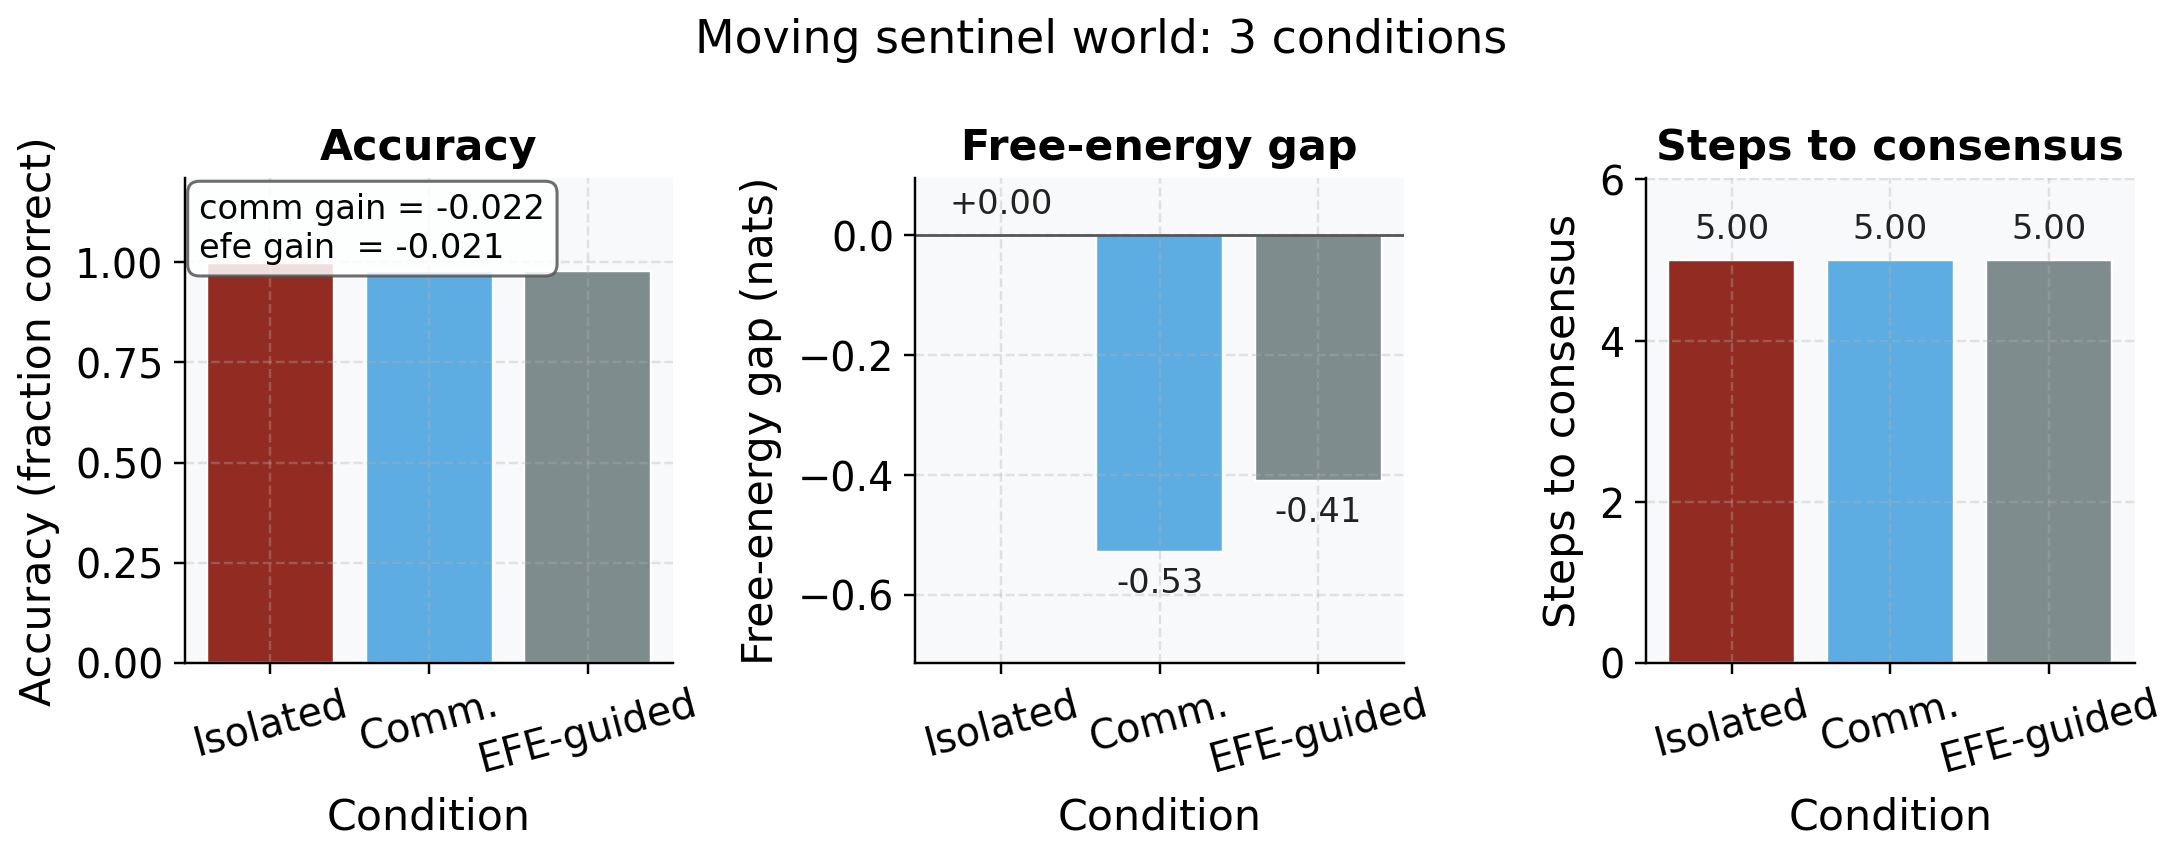
\includegraphics[width=0.8\linewidth,height=0.5\textheight,keepaspectratio,alt={Three-panel moving-world comparison of isolated, communicating, and expected-free-energy-guided conditions, showing accuracy, signed free-energy gap, and steps to consensus.}]{../figures/moving_world.png}
\caption{Moving sentinel world across isolated, communicating, and
EFE-guided conditions. Source relation: original project schematic for
the moving-world protocol; estimand: condition-level consensus accuracy,
signed free-energy gap, and steps-to-consensus proxy in the stated
native units; uncertainty: deterministic seeded run, so no resampling
interval is shown. Moving sentinel world across the three conditions
(x-axis is condition: isolated, communicating, EFE-guided). Left panel:
y-axis shows consensus accuracy (fraction of 960 trials whose pooled
argmax matches the truth). Center panel: y-axis shows the signed
free-energy gap in nats (isolated surprise minus the condition's
surprise on the true state, so a positive value would mean lower free
energy than isolated; the measured gaps are negative, plotted against a
zero reference line and annotated per bar). Right panel: y-axis shows a
coarse steps-to-consensus proxy, with per-bar value annotations showing
the three conditions are essentially tied. Each colony runs 6 steps over
a 4-cell linear grid with 2 disjoint-FOV agents. No resampling interval
applies to this deterministic seeded run. The finite reduced world does
not establish a general communication benefit, an optimal movement
policy, or source-protocol replication.}\label{fig:moving-world}
\end{figure}

\subsubsection{Disjoint field-of-view
extension}\label{sec:results-disjoint-fov}

To test whether communication is necessary (not merely beneficial) when
observations are non-overlapping, we extend Study 5 to 3 agents each
observing a 2-position disjoint window of a 6-position state space
(chance-level accuracy 0.167).

Isolated agents achieve mean accuracy 0.35 --- above chance but far from
decisive, since no single agent can infer the global state from a
partial window alone. Communicating agents pool complementary beliefs to
reach 0.55 (gap 0.19).

This is now a powered result, not an illustrative point estimate. Across
128 independent seeds the isolated accuracy is 0.326 (95\% CI
0.320--0.332) and the communicating accuracy is 0.493 (95\% CI
0.487--0.499), both clearing the 0.167 chance baseline --- isolated
agents are \emph{not} at chance, since a partial FOV plus majority
voting still carries some signal.

The paired Wilcoxon signed-rank test (communicating vs.~isolated,
matched by seed) gives \(p = 9.35 \times 10^{-23}\), effect size
\(r = 1.000\) (large): communicating beats isolated on every one of the
128 seeds. This agreement saturates the rank-biserial effect at its
upper bound; it does not turn the reported Wilcoxon signed-rank p-value
into an exact paired sign-test probability. The paired mean gap and its
interval quantify the accuracy contrast in its native units.

Given isolated performance is above chance, the precise claim is not
that communication is \emph{logically} necessary for any signal at all,
but that it is necessary to approach the communicating-level accuracy
under fully disjoint observations: the gap between the two conditions is
significant, large, and reproducible, unlike the binary-complement
contrast above.

We separately quantify EFE-guided navigation rather than asserting an
unquantified ``widens the gap'' effect. In a matched but smaller-scale
disjoint-FOV movement-policy comparison (2 agents, 4-position
binary-state grid, belief sharing active in both arms), EFE-guided
accuracy is 0.975 versus 0.977 for random movement (\(p = 0.1046\),
negligible effect). This comparison did not resolve an accuracy
difference in the configured near-ceiling regime with belief sharing
active; it does not establish equivalence of the movement policies.

We report this as the null result it is rather than claiming an
unmeasured EFE benefit. fig.~\ref{fig:disjoint-fov-world} summarizes the
necessity result.

\begin{figure}
\centering
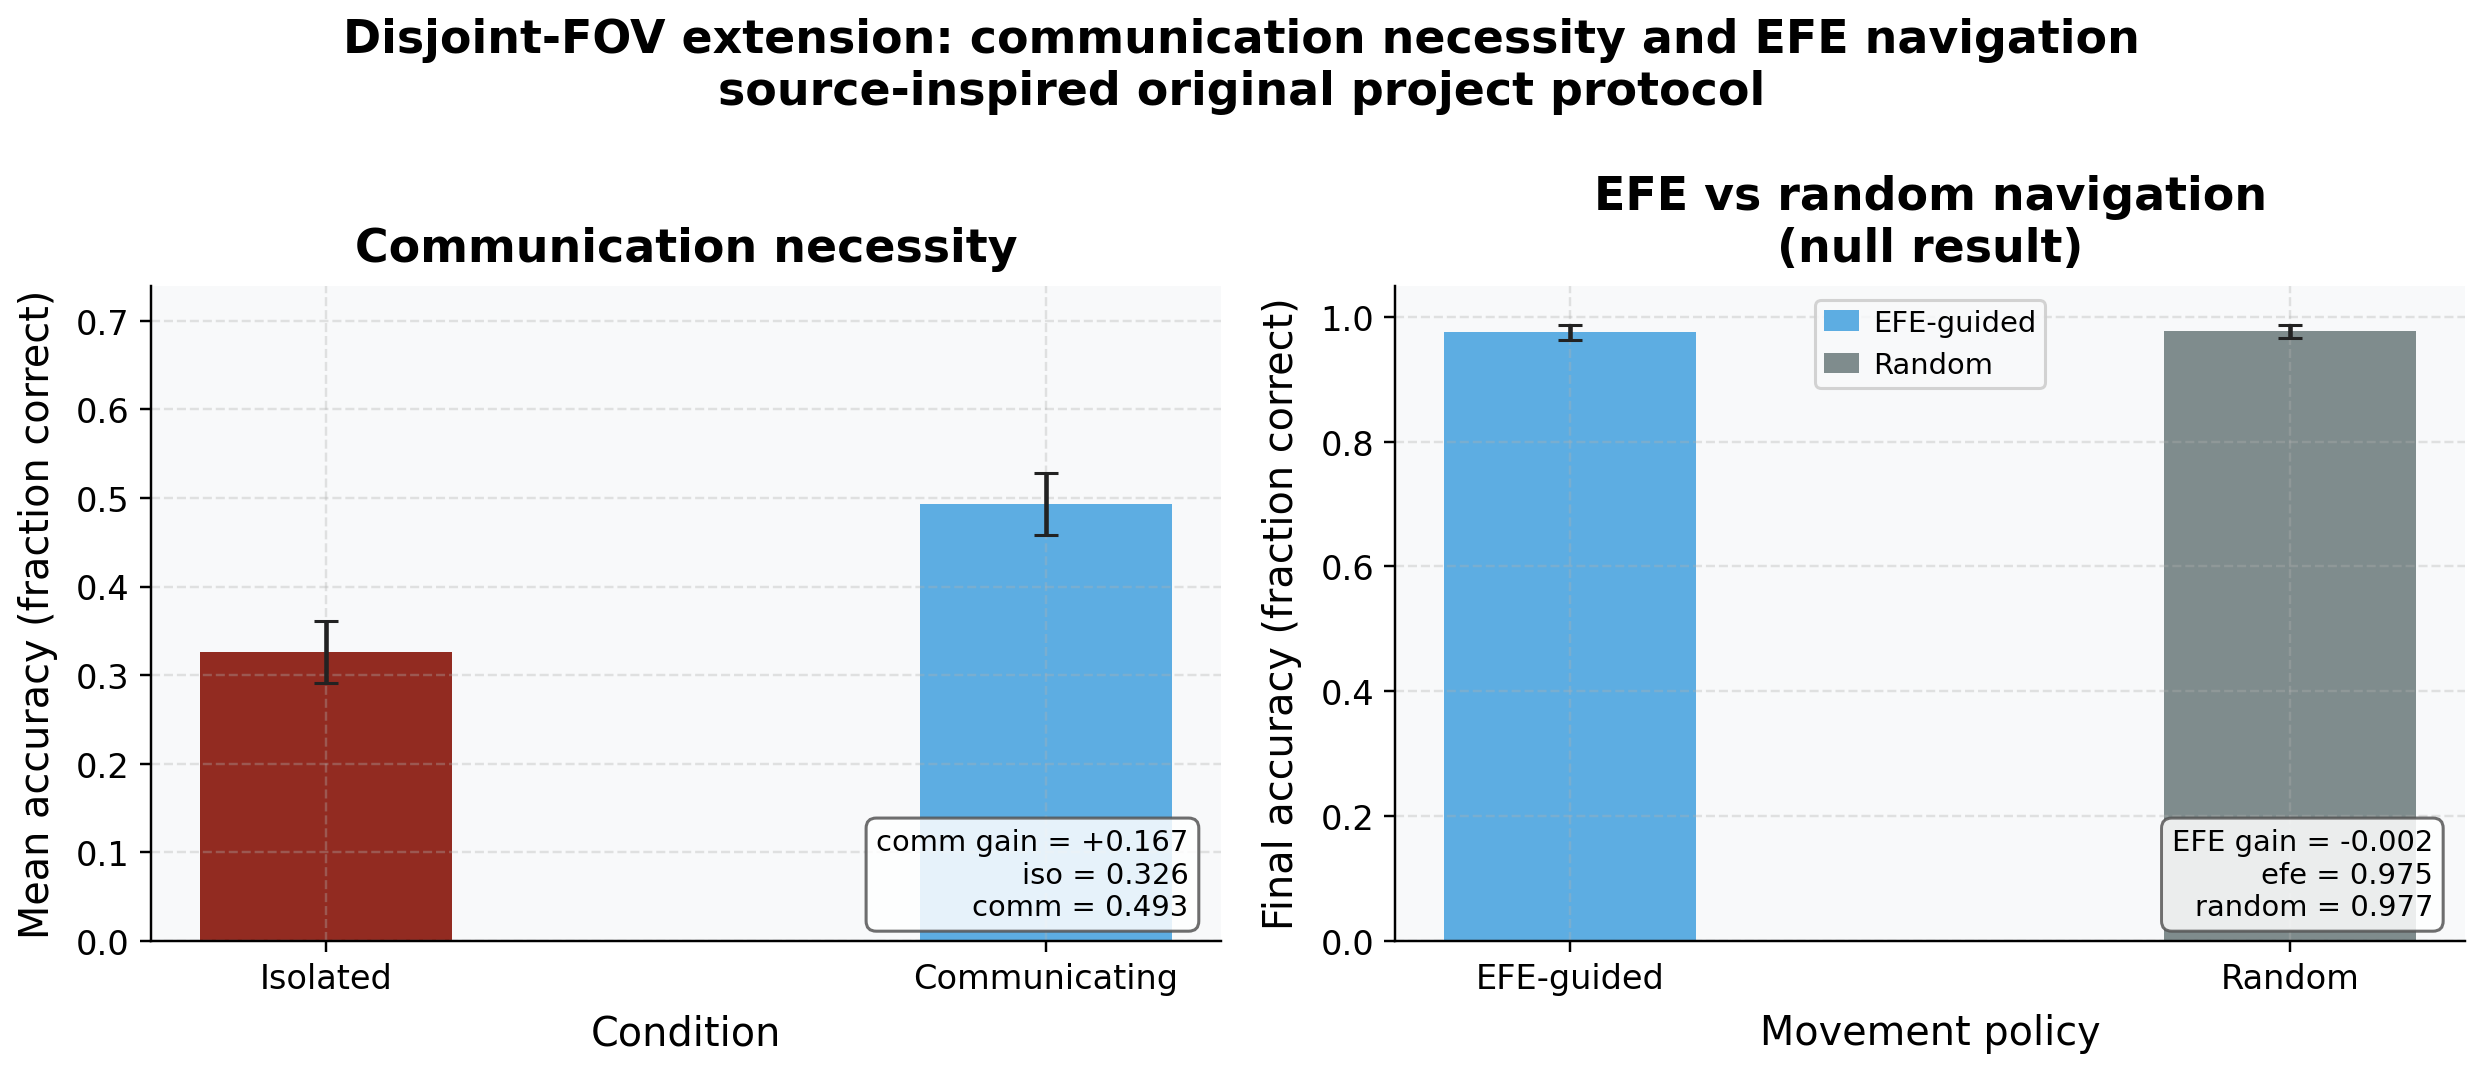
\includegraphics[width=0.8\linewidth,height=0.5\textheight,keepaspectratio,alt={Two-panel disjoint-field-of-view diagnostic. The left bars compare isolated and communicating consensus accuracy; the right bars compare EFE-guided and random movement, where both policies are near ceiling.}]{../figures/disjoint_fov_world.png}
\caption{Communication improves the declared disjoint-view condition,
whereas the configured movement-policy contrast is near-ceiling and
null. This is a source-inspired project extension of the moving-world
mechanism, produced from two separately configured reports. Source
relation: original project extension of the source-inspired moving-world
mechanism. Estimand: condition-level final consensus accuracy. Read left
to right. Panel A compares isolated and communicating consensus for 3
agents, each observing a non-overlapping 2-position window of a
6-position world. Panel B compares EFE-guided and random movement for 2
agents in a 4-position world. The x-axis is the condition or movement
policy; the y-axis is final consensus accuracy, the fraction of trials
whose pooled argmax equals the true state. Direct x-axis labels,
distinct hatches, dark keylines, and printed summary boxes duplicate
color. Bars are means across independent configured seeds; error bars
are across-seed standard deviations, not confidence intervals. Trials
and agents are nested within each seed. The paired Wilcoxon results are
\(p = 9.35 \times 10^{-23}\) for Panel A and \(p = 0.1046\) for Panel B.
The first supports only the configured communication contrast; the
second records the observed null rather than an EFE benefit. The panels
do not establish universal communication necessity, movement-policy
superiority, causal mechanism, or generalization beyond the declared
worlds and seed schedule.}\label{fig:disjoint-fov-world}
\end{figure}

\subsection{Supplement: moving-world methods and condition
definitions}\label{sec:supp-moving}

This supplement supplies the construction that
sec.~\ref{sec:results-moving} defers here: exactly how the
moving-sentinel world is built, how the three actions and the
expected-free-energy policy move an agent, and how the \emph{isolated},
\emph{communicating}, and \emph{EFE-guided} conditions differ.

It answers the mechanical question left open in the main section ---
what precisely is held fixed and what varies across the three conditions
whose accuracies are contrasted there --- so the reported
binary-complement numbers can be read against their generative model
rather than taken on trust.

The moving-world generative model is built by
\breaktt{build\_moving\_world}. A linear grid of 4 cells holds one binary
hidden state --- the half of the grid (left = state 0, right = state 1)
that contains the threat.

The 2 sentinels start at evenly tiled positions
(\(i \cdot \lfloor n_{\text{positions}} / n_{\text{agents}} \rfloor\))
and each observe a half-open field-of-view window. With the default
setup the two FOVs are disjoint, one per half.

Each agent's likelihood is a \(2 \times 2\) matrix over outcomes
(detected / not\_detected) given the binary state, with a confident
signed reading for the half the agent watches; the transition tensor
encodes three deterministic control paths --- stay, left (reflecting at
cell 0), and right (reflecting at the last cell). The hidden-state prior
is uniform.

Action selection has two regimes. The random conditions draw each
agent's move uniformly from the three controls. The EFE-guided condition
uses \breaktt{efe\_policy\_select}: for every candidate move it lands the
agent at the deterministic next position, reconstructs the likelihood
from that viewpoint, and scores the move by the expected posterior
entropy after one observation, \(H = \sum_o P(o)\,H(P(s \mid o))\) ---
taking the entropy-minimizing (information-seeking) step.

We compare three conditions --- \emph{isolated} (random moves, no
sharing), \emph{communicating} (random moves plus a per-step
log-linear-pool consensus), and \emph{EFE-guided} (information-seeking
moves plus the same per-step sharing) --- over 960 trials of 6 steps
each, scoring the pooled consensus against the true state. All numerics
are deterministic given the run seed.

\subsection{Hierarchical POMDP: federated belief sharing across
levels}\label{sec:results-hierarchical}

The flat sentinel world couples all agents at a single latent level ---
the creature's location.

A natural extension is a \textbf{2-level hierarchical POMDP} in which
location inference (Level 1, L1; 9 states) is coupled to a global
\emph{context} variable (Level 2, L2; 2 states: \texttt{quiet} /
\texttt{alert}) that modulates the L1 prior. In the \texttt{alert}
context the creature is expected near the den (center cell); in the
\texttt{quiet} context the prior is uniform.

Each sentinel runs alternating L1/L2 minimization with
\breaktt{hierarchical\_infer} from the \breaktt{fedference.pomdp} module
to infer both its location belief and the current context belief, then
the colony federates both levels via a log-linear pool.

We compare two conditions over 960 seeded trials with 4 agents at sensor
acuity 0.85:

\begin{itemize}
\tightlist
\item
  \textbf{Flat} --- agents ignore the hierarchy and infer location under
  a uniform prior;
\item
  \textbf{Hierarchical} --- agents run 4 alternating-minimization
  iterations to couple L1 and L2 beliefs before federating.
\end{itemize}

The measured location accuracies are 0.982 (flat) and 0.969
(hierarchical), a gap of -0.014.

Across 128 independent seeds the hierarchical location accuracy is 0.974
(SD 0.005; 95 \% CI 0.973--0.975) versus flat 0.982 (95 \% CI
0.981--0.982), a mean accuracy gap of -0.008 (95 \% CI -0.009---0.007;
Wilcoxon signed-rank \(p = 3.59 \times 10^{-20}\), effect size
\(r = 0.940\), large).

On location the gap is small but statistically reliable in the
\emph{negative} direction --- the paired test rejects at
\(\alpha = 0.05\) and the gap's confidence interval (-0.009---0.007)
excludes zero on the negative side --- so the hierarchy does not improve
location accuracy in this regime; if anything it pays a small,
consistent location cost for carrying the extra latent level.

Its added value is that it \emph{also} infers the context latent, at
accuracy 0.763 against a two-state chance baseline of \(0.5\). Two-level
federation therefore runs L1/L2 inference end-to-end and resolves
context above chance while paying a small, reliable location cost
relative to the flat baseline (fig.~\ref{fig:hierarchical-pomdp}).

Context beliefs across the alternating-minimization iterations are shown
in the top-middle panel: P(alert) sits above the two-state chance line
and is stable from the first iteration onward when the observed location
is the center cell --- the center-cell observation pins the context
posterior immediately, because the alert context-conditioned L1 prior is
peaked there.

The full construction and parameter sweep are detailed in the supplement
(sec.~\ref{sec:supp-hierarchical}). For the effect of acuity and colony
size on these results, see sec.~\ref{sec:results-sensitivity}.

\begin{figure}
\centering
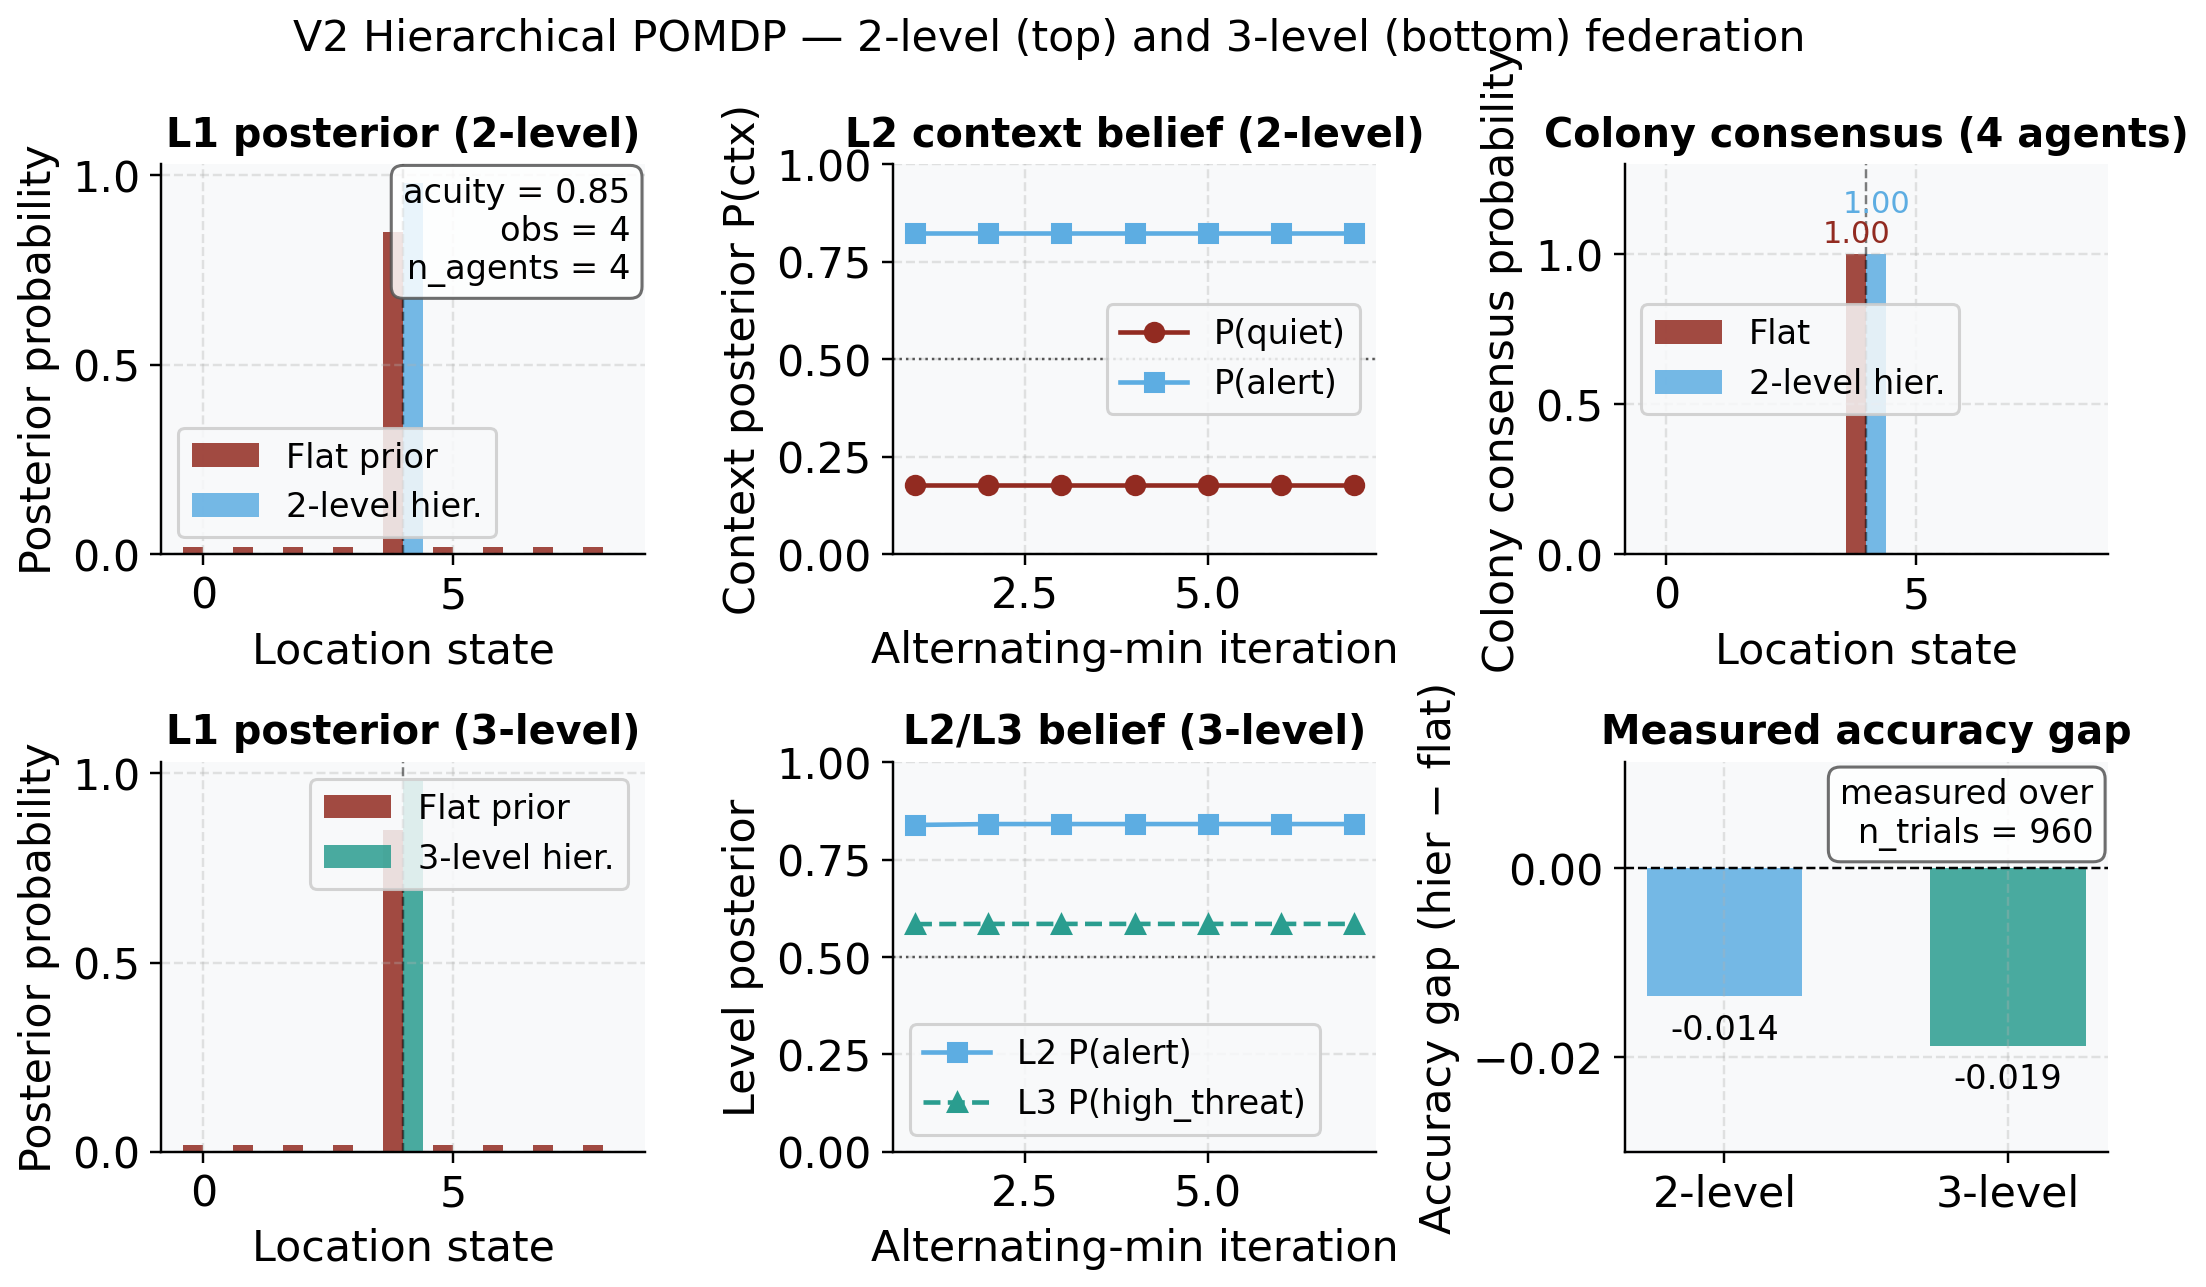
\includegraphics[width=0.8\linewidth,height=0.5\textheight,keepaspectratio,alt={Six-panel hierarchical POMDP diagnostic. The top row shows two-level location, context, and colony beliefs; the bottom row shows three-level beliefs and measured hierarchical-minus-flat accuracy gaps. Plain and forward-hatched bars, distinct trajectory markers, peak labels, and direct signed values duplicate color.}]{../figures/hierarchical_pomdp.png}
\caption{Six-panel hierarchical POMDP belief-dynamics and accuracy
diagnostic. Source relation: source-inspired original project diagnostic
for a hierarchical extension; estimand: posterior probabilities and
final hierarchical-minus-flat location-accuracy gap in the declared
seeded protocol. Read the two-level world across the top row and the
three-level extension across the bottom. In the left column, the x-axis
indexes 9 location states and the y-axis is posterior probability after
one center-cell observation; plain left-offset bars are the flat-prior
reference and forward-hatched right-offset bars are hierarchical. In the
middle column, the x-axis is alternating-minimization iteration and the
y-axis is context probability; circles, squares, triangles, and solid or
dashed paths identify the displayed levels without color. The top-right
panel uses the same plain-versus-hatched bar grammar for L1 consensus
after federating 4 agents, with direct peak labels. The bottom-right
panel's x-axis is hierarchy depth and its y-axis is the final
accuracy-fraction contrast over 960 nested trials, with direct signed
values and a zero rule. Units are probability or accuracy fraction. Seed
0 defines one deterministic protocol realization; ordered states,
iterations, agents, and trials are nested measurements rather than
independent resampling units, so no interval or error band applies. The
figure does not establish universal hierarchical benefit, calibrated
uncertainty, or source-protocol
replication.}\label{fig:hierarchical-pomdp}
\end{figure}

\subsection{Supplement: hierarchical POMDP methods and
parameters}\label{sec:supp-hierarchical}

This supplement makes the two-level construction of
sec.~\ref{sec:results-hierarchical} concrete: how location (L1) is
coupled to context (L2) through context-conditioned priors, what the
alternating-minimization update actually computes, and the exact
parameters of the executed run.

It answers the question the main section brackets --- \emph{by what
mechanism does a second latent level enter the inference at all} --- and
thereby fixes why the hierarchy resolves context above chance while
retaining the separate location-accuracy contrast reported in
sec.~\ref{sec:results-hierarchical}.

\subsubsection{Generative model for context-gated location
inference}\label{generative-model-for-context-gated-location-inference}

The two-level POMDP is built by \breaktt{build\_hierarchical\_world} in
the \breaktt{fedference.pomdp} module. It couples the sentinel's
9-location L1 factor to a 2-state L2 context factor via
\textbf{context-conditioned L1 priors}.

\textbf{L1 (location).} The standard 3x3 grid of
\breaktt{build\_sentinel\_world} has \texttt{n\_s\ =} 9 states and sensor
acuity 0.85.

\textbf{L2 (context).} A binary \texttt{quiet} / \texttt{alert} state
has a symmetric transition matrix with persistence 0.90 and an initial
uniform prior.

\textbf{L1 priors given context.} \texttt{quiet} is uniform over all 9
cells. \texttt{alert} places mass 0.60 at the center cell (the den) and
spreads the residual uniformly.

\subsubsection{Inference algorithm for top-down empirical
priors}\label{inference-algorithm-for-top-down-empirical-priors}

The module's \breaktt{hierarchical\_infer} function performs 4 passes of
alternating minimization:

\textbf{1. L2 \texorpdfstring{\ensuremath{\to}}{->} L1 empirical prior.} \(\widetilde{\pi}_{0,\mathrm{L1}} =
\sum_c q_{\text{ctx}}[c]\,\pi_{0,\mathrm{L1}\mid c}\), a soft mixture of
the two context-conditioned priors.

\textbf{2. L1 update.} The one-step variational posterior is
\(q_{\text{loc}} = \operatorname{softmax}(\log \widetilde{\pi}_{0,\mathrm{L1}} +
\log A[\text{obs},\,\cdot])\).

\textbf{3. L1 \texorpdfstring{\ensuremath{\to}}{->} L2 marginal evidence.}
\(\ell_c = \log\bigl(\pi_{0,\mathrm{L1}\mid c}^{\top}
A[\text{obs},\,\cdot]\bigr)\), the evidence for context \(c\) from the
observed location likelihood.

\textbf{4. L2 update.}
\(q_{\text{ctx}} = \operatorname{softmax}(\log \pi_{0,\mathrm{L2}} + \ell)\).

After 4 iterations the agent broadcasts both \(q_{\text{loc}}\) and
\(q_{\text{ctx}}\); the colony federates each level independently via a
log-linear pool (eq.~\ref{eq:log-linear-pool}).

\subsubsection{Study parameters for the hierarchical
condition}\label{study-parameters-for-the-hierarchical-condition}

\begin{longtable}[]{@{}ll@{}}
\caption{Study 6 hierarchical POMDP execution parameters: agent count,
seeded trial budget, observation acuity, alternating-minimization
iterations, and the L2/L1 state cardinalities used by the two-level
condition.}\label{tbl:hier-params}\tabularnewline
\toprule\noalign{}
Parameter & Value \\
\midrule\noalign{}
\endfirsthead
\toprule\noalign{}
Parameter & Value \\
\midrule\noalign{}
\endhead
\bottomrule\noalign{}
\endlastfoot
Agents & 4 \\
Trials & 960 \\
Acuity & 0.85 \\
Alternating-min iterations & 4 \\
L2 context states & 2 \\
L1 location states & 9 \\
Seed & 0 \\
\end{longtable}

The executed hierarchical configuration is summarized in
tbl.~\ref{tbl:hier-params}.

\subsection{Three-level hierarchical POMDP: an executed test of the
N-level template}\label{sec:results-3level}

The 2-level hierarchical POMDP (sec.~\ref{sec:results-hierarchical})
couples location inference to a single global context. The N-level
architecture uses \breaktt{build\_nlevel\_world} from the
\breaktt{fedference.pomdp} module and provides a parameterized stack of
levels; the canonical 3-level example couples location (L1; 9 states) to
a context variable (L2; 2 states: \texttt{quiet} / \texttt{alert}) and
further to a meta-context variable (L3; 2 states: \texttt{low\_threat} /
\texttt{high\_threat}) that gates the L2 prior.

\begin{equation}\protect\phantomsection\label{eq:l3-to-l2-message}{
\tilde{D}_{\text{L2}} = \sum_k q_{\text{L3}}[k]\,p_{\text{L2|L3}}[k]
}\end{equation}

\begin{equation}\protect\phantomsection\label{eq:l2-to-l1-message}{
\tilde{D}_{\text{L1}} = \sum_c q_{\text{L2}}[c]\,p_{\text{L1|L2}}[c]
}\end{equation}

The inference algorithm (\breaktt{fedference.pomdp.nlevel\_infer})
performs 4 passes of top-down / bottom-up alternating minimization: the
top-down pass propagates empirical priors from L3 \texorpdfstring{\ensuremath{\to}}{->} L2 \texorpdfstring{\ensuremath{\to}}{->} L1 via
eq.~\ref{eq:l3-to-l2-message} and eq.~\ref{eq:l2-to-l1-message}; the
bottom-up pass updates each level's belief from the marginal evidence
contributed by the level below.

We compare two conditions over 960 seeded trials with 4 agents at sensor
acuity 0.85.

\textbf{Flat condition.} Agents ignore all hierarchy and infer location
under a uniform prior.

\textbf{Three-level condition.} Agents run 4 alternating-minimization
iterations across all three levels before federating.

The measured location accuracies are 0.984 (flat) and 0.966 (3-level), a
gap of -0.019.

Across 128 independent seeds the 3-level location accuracy is 0.976 (SD
0.005; 95 \% CI 0.976--0.977) versus flat 0.981 (95 \% CI 0.980--0.981),
a mean accuracy gap of -0.004 (95 \% CI -0.005---0.003; Wilcoxon
signed-rank \(p = 2.88 \times 10^{-12}\), effect size \(r = 0.724\),
medium). The signed mean gap and its interval describe the
location-accuracy cost of this configured three-level condition relative
to the flat baseline.

The 3-level condition additionally reports context accuracy 0.697 and
meta-context accuracy 0.547.

Against the two-state chance baseline of \(0.5\), location is recovered
and the intermediate context latent is resolved well above chance, but
the meta-context latent is only marginally above chance --- the weakest
of the three levels --- and is therefore \emph{not} convincingly
recovered here.

The study thus demonstrates that the generic \(N\)-level
alternating-minimization runs and federates end-to-end and recovers the
fastest (location) and intermediate (context) latents; full recovery of
the slowest (meta-context) level is left open.

The full figure comparing 2-level and 3-level belief dynamics is
fig.~\ref{fig:hierarchical-pomdp}. The declarative layer specification
used by the generic constructor is documented in the supplement
(sec.~\ref{sec:supp-3level}). For the effect of acuity and colony size
on these results, see sec.~\ref{sec:results-sensitivity}.

\subsection{Supplement: N-level hierarchical POMDP
methods}\label{sec:supp-3level}

This supplement specifies the generic \(N\)-level architecture that
sec.~\ref{sec:results-3level} exercises at depth three: how the
meta-context (L3), context (L2), and location (L1) factors are chained
through conditioned priors, what the declarative \texttt{LayerSpec}
interface fixes versus leaves free, and the top-down/bottom-up passes
the inference runs.

It answers \emph{what the executed 3-level result is a special case of}
--- the reason the same code runs at other depths without new
mathematics --- while recording that only the declared 3-level
configuration is empirically evaluated here.

\subsubsection{Generative model for an N-level
hierarchy}\label{generative-model-for-an-n-level-hierarchy}

The 3-level POMDP is built by \breaktt{build\_3level\_world} in the
\breaktt{fedference.pomdp} module. It extends the 2-level construction
(sec.~\ref{sec:supp-hierarchical}) by adding a top-level meta-context
factor.

\textbf{L3 (meta-context).} 2 \texttt{low\_threat} /
\texttt{high\_threat} states begin from a uniform prior and gate the L2
context prior.

\textbf{L2 (context).} 2 \texttt{quiet} / \texttt{alert} states gate the
L1 prior through context-conditioned location priors.

\textbf{L1 (location).} The standard 3x3 grid has 9 states and sensor
acuity 0.85.

The conditioned priors are (see eq.~\ref{eq:l3-to-l2-message} and
eq.~\ref{eq:l2-to-l1-message}):

{\def\LTcaptype{none} % do not increment counter
\begin{longtable}[]{@{}ll@{}}
\toprule\noalign{}
L3 state & L2 prior (quiet, alert) \\
\midrule\noalign{}
\endhead
\bottomrule\noalign{}
\endlastfoot
\texttt{low\_threat} & (0.50, 0.50) --- uniform context \\
\texttt{high\_threat} & (0.20, 0.80) --- peaked at alert \\
\end{longtable}
}

{\def\LTcaptype{none} % do not increment counter
\begin{longtable}[]{@{}
  >{\raggedright\arraybackslash}p{(\linewidth - 2\tabcolsep) * \real{0.5000}}
  >{\raggedright\arraybackslash}p{(\linewidth - 2\tabcolsep) * \real{0.5000}}@{}}
\toprule\noalign{}
\begin{minipage}[b]{\linewidth}\raggedright
L2 state
\end{minipage} & \begin{minipage}[b]{\linewidth}\raggedright
L1 prior
\end{minipage} \\
\midrule\noalign{}
\endhead
\bottomrule\noalign{}
\endlastfoot
\texttt{quiet} & uniform over all 9 location states \\
\texttt{alert} & mass 0.60 at center cell (flat index 4), residual
uniform \\
\end{longtable}
}

\subsubsection{Generic N-level
architecture}\label{generic-n-level-architecture}

The \texttt{LayerSpec} type and \breaktt{build\_nlevel\_world} function
in the \breaktt{fedference.pomdp} module implement the generic N-level
version. The declarative layer specification is
\breaktt{hierarchical\_layers.yaml} under
\breaktt{src/fedference/config/}; it mirrors the canonical 3-level
defaults (a standalone documentation artifact not read by any code path,
kept in sync with the \breaktt{build\_3level\_world} defaults).

The constructor accepts depth \texorpdfstring{\textgreater{}=}{>=} 2; the executed empirical result in this
manuscript is restricted to the declared 3-level configuration, and the
leaf layer must carry \breaktt{n\_states\ ==\ N\_LOCATIONS}.

\subsubsection{Inference algorithm across hierarchy
levels}\label{inference-algorithm-across-hierarchy-levels}

\breaktt{fedference.pomdp.nlevel\_infer} performs 4 passes of top-down /
bottom-up alternating minimization over all N levels:

\textbf{1. Top-down pass.} Compute the empirical prior for each level by
marginalizing over the level above (eq.~\ref{eq:l3-to-l2-message},
eq.~\ref{eq:l2-to-l1-message}).

\textbf{2. L1 update.} The one-step variational posterior on the
observation is
\(q_{\text{loc}} = \operatorname{softmax}(\log \widetilde{\pi}_{0,\mathrm{L1}} +
\log A[\text{obs},\,\cdot])\).

\textbf{3. Bottom-up pass.} Update each non-leaf level's belief from the
marginal evidence contributed by the level below:
\(\ell_j = \log(\tilde{p}_{\text{child|parent=}j}^\top q_{\text{child}})\).

After 4 iterations the agent broadcasts all N level beliefs; the colony
federates each level independently via a log-linear pool
(eq.~\ref{eq:log-linear-pool}).

\subsubsection{Study parameters for the three-level
run}\label{study-parameters-for-the-three-level-run}

\begin{longtable}[]{@{}ll@{}}
\caption{Study 7 three-level hierarchical POMDP execution parameters:
agent count, seeded trial budget, observation acuity,
alternating-minimization iterations, and the L3/L2/L1 state
cardinalities used by the three-level
condition.}\label{tbl:nlevel3-params}\tabularnewline
\toprule\noalign{}
Parameter & Value \\
\midrule\noalign{}
\endfirsthead
\toprule\noalign{}
Parameter & Value \\
\midrule\noalign{}
\endhead
\bottomrule\noalign{}
\endlastfoot
Agents & 4 \\
Trials & 960 \\
Acuity & 0.85 \\
Alternating-min iterations & 4 \\
L3 meta-context states & 2 \\
L2 context states & 2 \\
L1 location states & 9 \\
Seed & 0 \\
\end{longtable}

The executed three-level configuration is summarized in
tbl.~\ref{tbl:nlevel3-params}.

\subsection{Signed accuracy contrasts over acuity and colony
size}\label{sec:results-sensitivity}

Studies 1--7 fix specific parameter configurations (sensor acuity and
colony size) to isolate mechanistic claims. Study 8 asks how the
communicating-minus- isolated and hierarchical-minus-flat accuracy
contrasts vary across a systematic two-dimensional sweep. This
estimand-first formulation makes sign changes visible without presuming
that either architecture is uniformly advantageous.

We sweep sensor acuity \(\kappa \in \{0.40, 0.55, 0.70, 0.85, 0.95\}\)
and colony size \(n \in \{2, 4, 6, 8, 10\}\), evaluating two systems:

\begin{itemize}
\tightlist
\item
  \textbf{Belief sharing} (Study 1 architecture) --- accuracy gap =
  communicating minus isolated mean accuracy;
\item
  \textbf{Hierarchical POMDP} (Study 6 architecture) --- accuracy gap =
  hierarchical minus flat location accuracy.
\end{itemize}

Each cell averages \(n_{\text{trials}} = 20\) independent trials to
reduce Monte-Carlo noise at the cell level.

The resulting heatmaps (fig.~\ref{fig:sensitivity-heatmap}) show the
accuracy gap for both systems as a function of acuity and colony size.
The signed scale is centered on zero: brown cells encode positive gaps,
blue cells encode negative gaps, and the neutral midpoint encodes zero.
Every cell also prints its signed value, so the direction remains
explicit without color. Hatching identifies only the declared
\(|\mathrm{gap}| \le 0.05\) display band; it is not an unreliability
flag, confidence interval, significance test, or proof of zero effect.

Across the grid the following patterns hold:

\subsubsection{Pattern 1: low-to-moderate
acuity}\label{pattern-1-low-to-moderate-acuity}

\textbf{Positive communicating-minus-isolated contrasts occur at
low-to-moderate acuity.} The accuracy gap peaks in the second-lowest
acuity row, where observations carry some signal but no single sentinel
resolves the location alone. It remains positive across the two
lowest-acuity rows for colonies of at least four agents in the declared
grid.

Near ceiling acuity the gap approaches zero because isolated agents
already solve most trials in the declared task.

\subsubsection{Pattern 2: a colony-size
floor}\label{pattern-2-a-colony-size-floor}

\textbf{Colony size acts through a floor, not a smooth slope.} The
two-agent column shows an exactly zero belief-sharing gap at every
acuity. Under self-exclusion (``agents do not hear themselves''), each
member hears exactly one incoming belief, so the heard consensus adds no
pooled evidence. Colonies of four or more show the positive low-acuity
contrast within this grid.

\subsubsection{Pattern 3: a conditional hierarchical
contrast}\label{pattern-3-a-conditional-hierarchical-contrast}

\textbf{The hierarchical contrast changes with acuity and colony size.}
Negative hierarchical-minus-flat location-accuracy gaps occur across the
lower-acuity rows, including colonies larger than two agents. The
higher-acuity rows are near zero outside the two-agent column; positive
cells are confined to that column in this grid. This conditional pattern
does not establish a general hierarchical accuracy advantage, and the
per-study paired location contrast remains a separate estimate under its
own trial and seed budget.

The full parameter grid and protocol details are in the supplement
(sec.~\ref{sec:supp-sensitivity}). A native-unit cross-study overview of
the headline metrics across all 9 studies is shown in
fig.~\ref{fig:cross-study-summary}.

Read the page-compatible composition down the full left column and then
down the right: Panel A contains the six accuracy rows, Panel B at upper
right the two information or free-energy rows, and Panel C at lower
right the single recovery row. Each study appears once, in its
applicable native-unit panel.

\begin{figure}
\centering
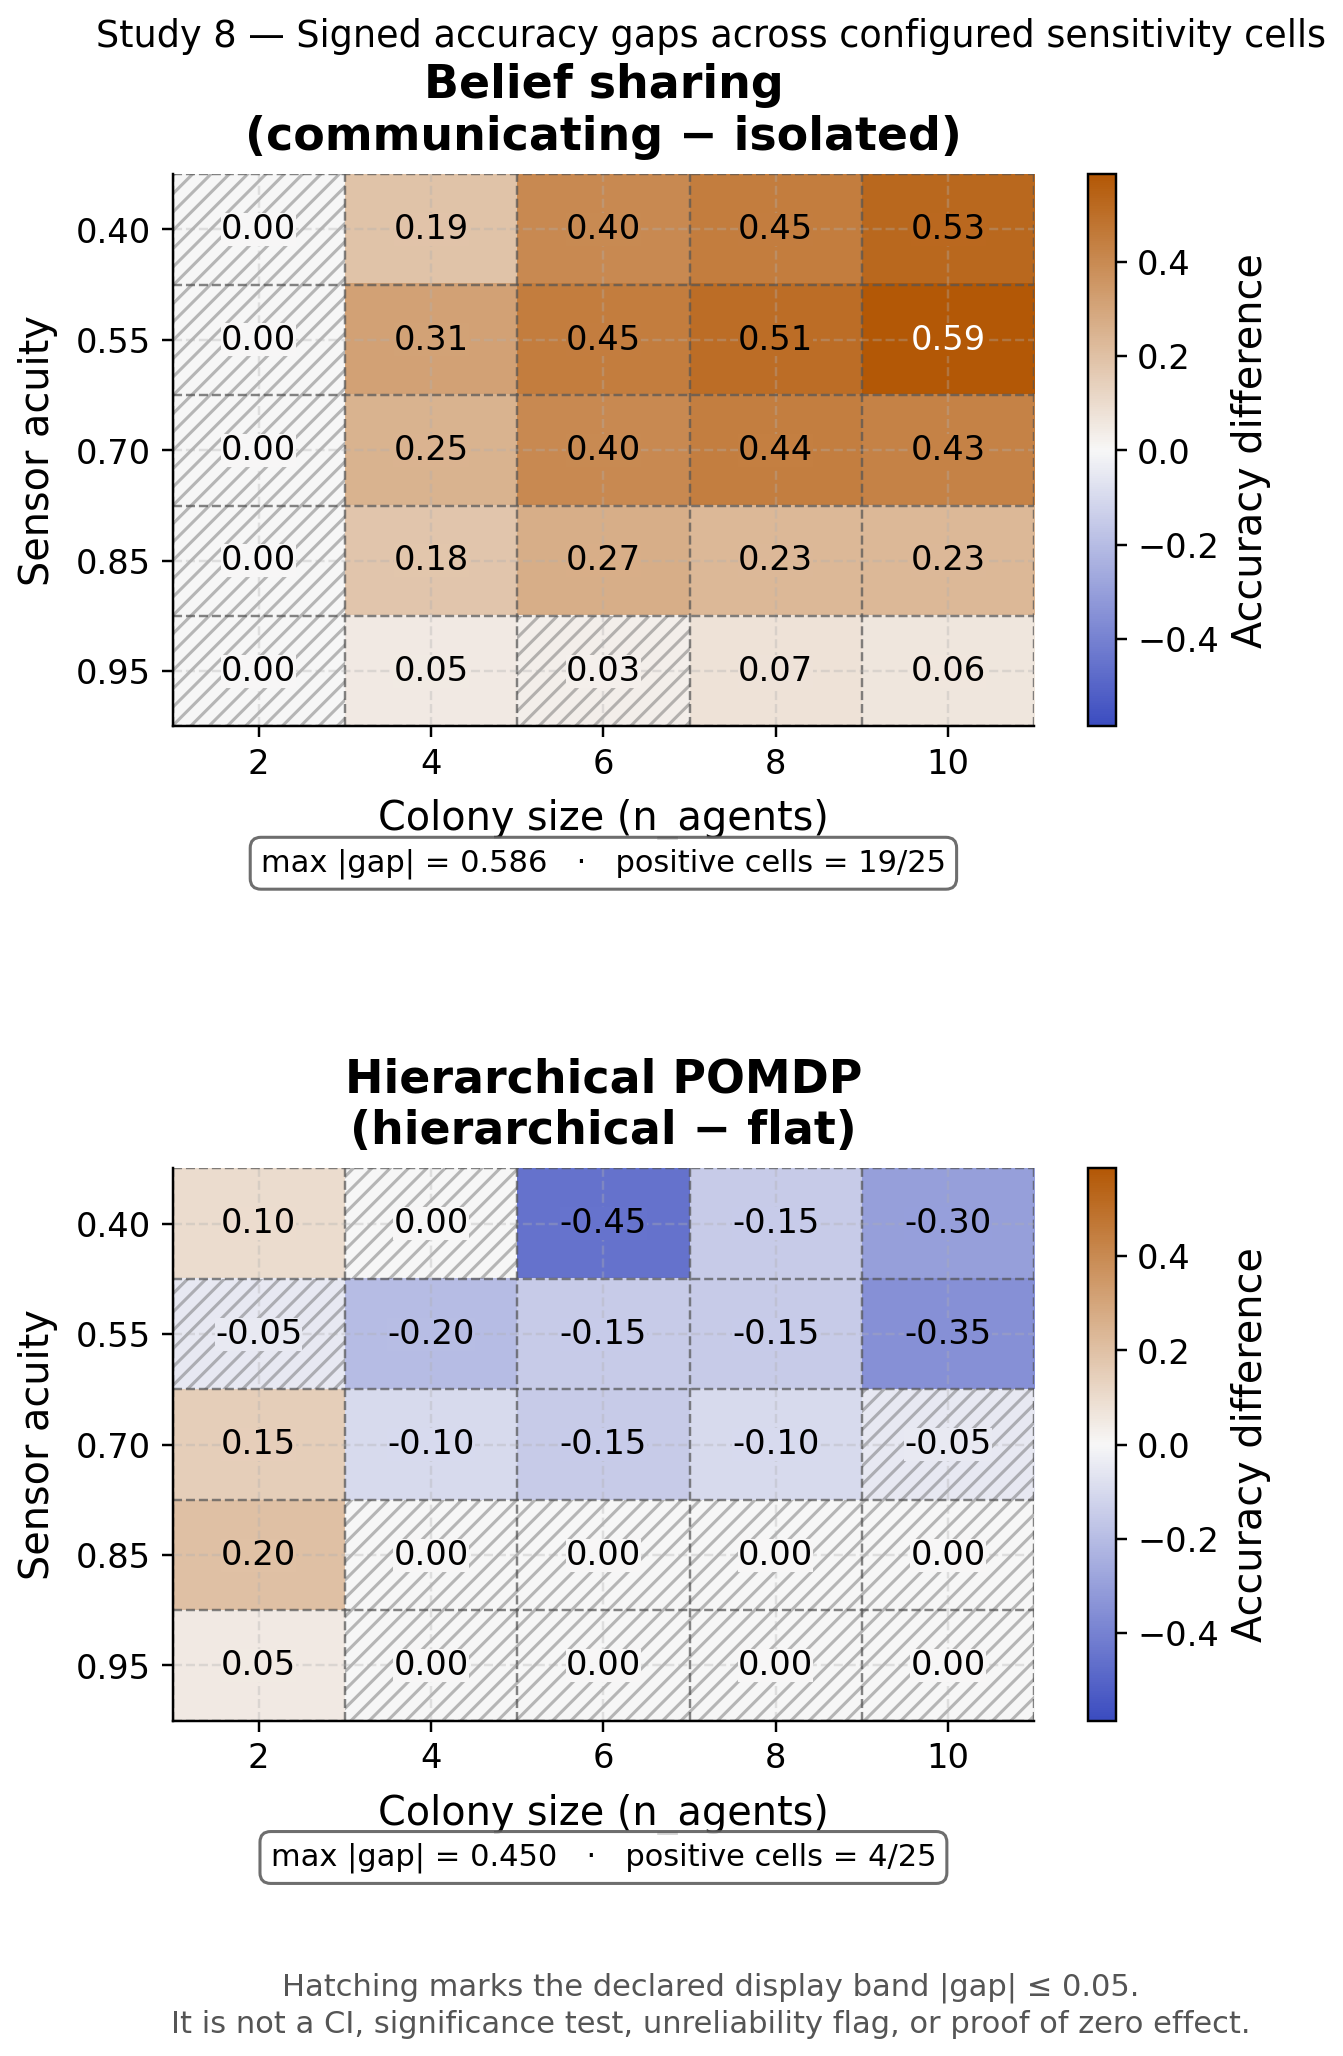
\includegraphics[width=0.9\linewidth,height=0.5\textheight,keepaspectratio,alt={Two heatmaps of accuracy gaps over sensor acuity and colony size: communicating minus isolated above, and hierarchical minus flat below. A symmetric color scale is centered at zero and hatched cells mark the declared display band using unrounded gaps. Printed values are rounded, so equal printed values can have different hatching; the band is not a confidence interval.}]{../figures/sensitivity_heatmap.png}
\caption{Two-panel sensitivity heatmap of belief-sharing and
hierarchical accuracy gaps. Source relation: original project
sensitivity diagnostic; estimand: per-cell accuracy gaps (fractions) as
functions of acuity and colony size; uncertainty: deterministic per-cell
means over the declared trials, with no resampling interval. Two
vertically stacked heatmaps of the Study 8 parameter sensitivity sweep.
Upper panel: y-axis indexes sensor acuity (0.40--0.95, 5 levels); x-axis
indexes colony size (2--10 agents, 5 levels); color encodes the
belief-sharing accuracy gap (communicating minus isolated mean
accuracy). Lower panel: identical axes; color encodes the hierarchical
POMDP location accuracy gap (hierarchical minus flat). The zero-centered
blue--neutral--brown scale encodes negative, zero, and positive gaps,
respectively; printed signed values provide the non-color encoding.
Diagonal hatching marks the declared \(|\mathrm{gap}| \le 0.05\) display
band using unrounded gaps. Printed cell values are rounded, so equal
printed values can have different hatching. The hatch is not an
unreliability designation, confidence interval, significance test, or
proof of zero effect. Cell values are deterministic per-cell means over
20 trials; trials are nested within their configured cell, and no
resampling interval is shown. The sweep protocol is detailed in the
sensitivity supplement, and the finite grid does not establish a general
communication or hierarchy effect outside the declared acuity and
colony-size settings.}\label{fig:sensitivity-heatmap}
\end{figure}

\begin{figure}
\centering
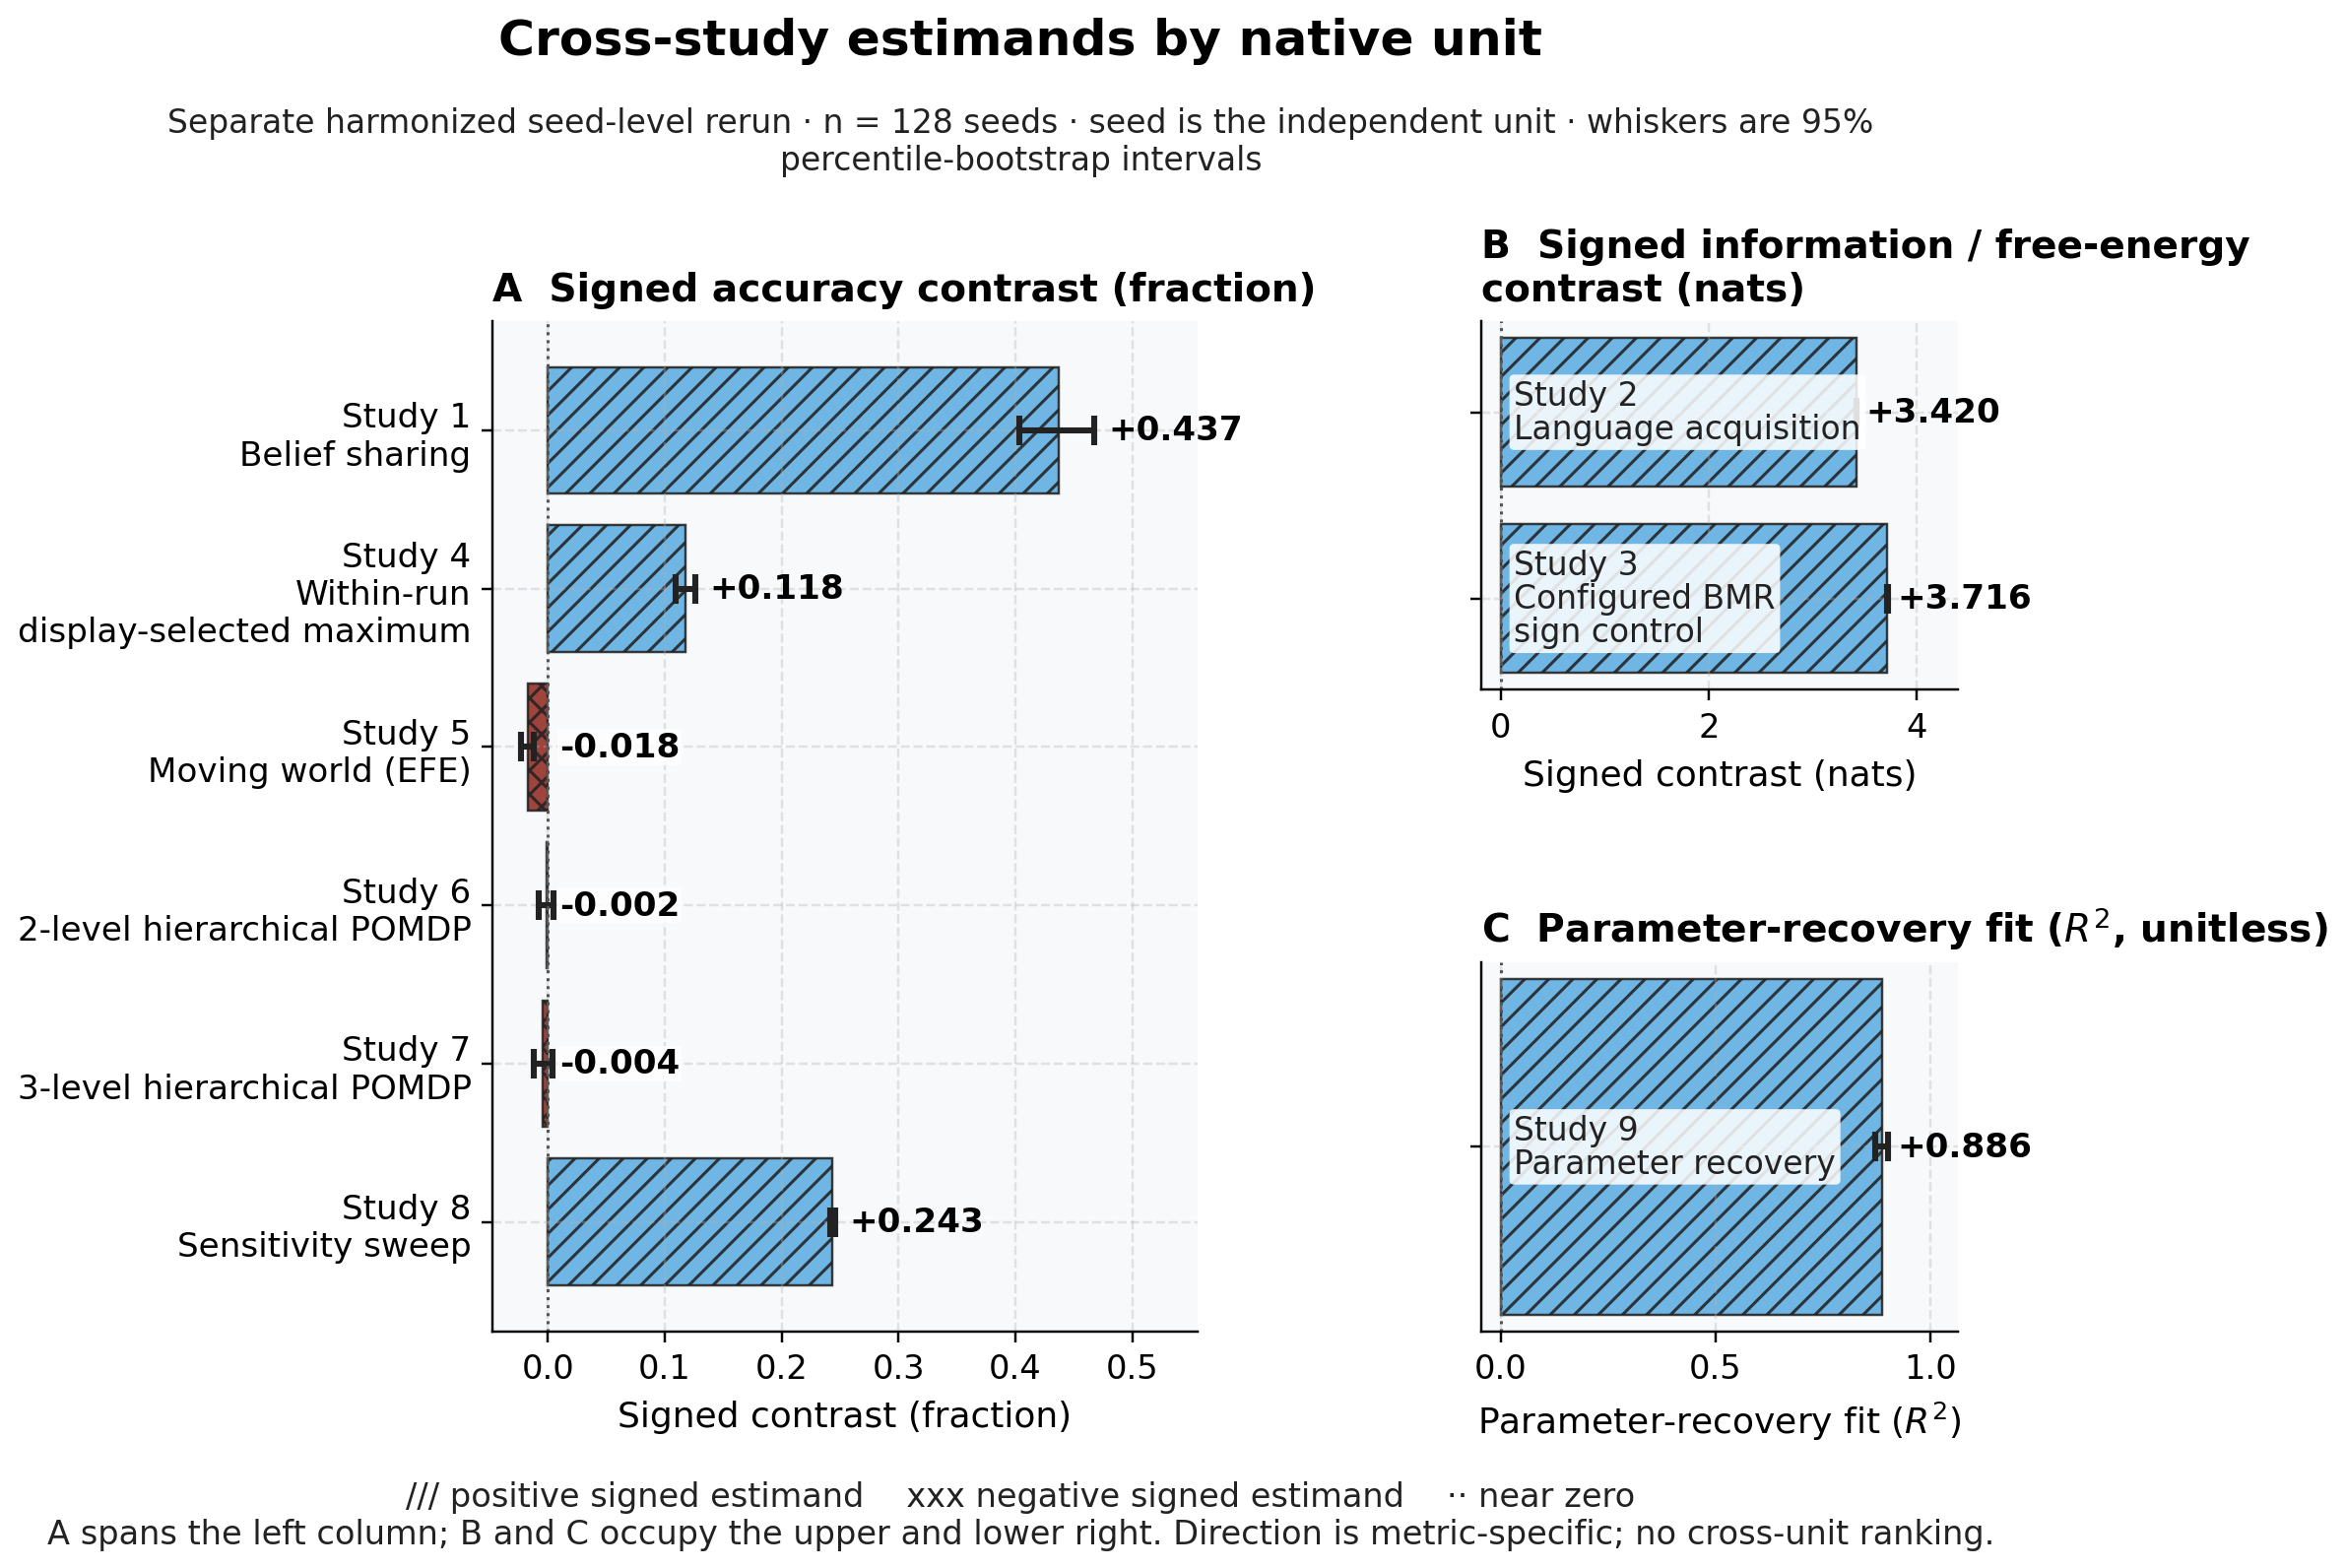
\includegraphics[width=0.95\linewidth,height=0.5\textheight,keepaspectratio,alt={A page-compatible two-column composition keeps native units separate: six signed accuracy rows span the left column, while information or free-energy rows in nats and one parameter-recovery R-squared row occupy the upper and lower right. Labels, whiskers, hatches, and zero rules duplicate color; intervals belong to a separate harmonized seed-level rerun.}]{../figures/cross_study_summary.png}
\caption{Native-unit cross-study summary of the headline signed
contrasts. Source relation: original-project synthesis from a separate
harmonized seed-level rerun; status: conditional overview, not a pooled
meta-analysis. Panel A, read down the left column, shows six signed
accuracy contrasts in fractions. Panel B at upper right shows two
information or free-energy contrasts in nats. Panel C at lower right
shows one parameter-recovery fit in unitless \(R^2\). Each x-axis
reports the signed study-level mean in its panel's native unit; each
y-axis lists only that panel's studies. Horizontal bars are means,
whiskers are 95\% percentile-bootstrap intervals, and direct signed
labels give the means. Forward, cross, and dotted hatches distinguish
positive, negative, and near-zero estimands; the dark dotted rule marks
zero without color. The independent and resampling unit is the seed
(\(n=128\)) within each configured study, with observations, agents,
trials, and ordered steps nested. These intervals belong only to the
harmonized rerun, including rows whose primary figure is a deterministic
single-posterior diagnostic; they do not retrofit uncertainty to those
primary figures. The Study 4 row is the within-run display-selected
maximum across non-reference server presets at the declared worst rate,
neither a preselected method nor an inferential winner. Native units are
preserved: the figure neither ranks nor pools studies nor implies a
shared effect or universal benefit.}\label{fig:cross-study-summary}
\end{figure}

\subsection{Supplement: parameter-sensitivity
methods}\label{sec:supp-sensitivity}

This supplement documents how the sensitivity grid of
sec.~\ref{sec:results-sensitivity} is generated and --- importantly for
a reader trying to reconcile numbers across studies --- where its two
sweeps use \emph{different} seeding and trial budgets. It answers two
questions the main section leaves implicit: exactly which seed drives
each cell, so every cell is deterministically reproducible in isolation;
and why the cross-study summary's sensitivity row is not directly
comparable, at matched trial counts, to the standalone heatmap.

\subsubsection{Experimental protocol for grid
sensitivity}\label{experimental-protocol-for-grid-sensitivity}

The sensitivity sweep uses \breaktt{run\_belief\_sharing\_sensitivity}
and \breaktt{run\_hierarchical\_sensitivity} from the
\breaktt{fedference.experiments} module. Each function accepts a tuple of
acuity values and a tuple of colony sizes. In the
\textbf{belief-sharing} sweep every (acuity, colony-size) cell averages
\(n_{\text{trials}}\) independent trials, each seeded via a
deterministic formula:

\begin{equation}\protect\phantomsection\label{eq:sensitivity-seed}{
\text{seed}_{\text{cell}} = \text{seed}_{\text{base}} + i \cdot 10^5 + j \cdot 10^3 + t
}\end{equation}

where \(i\) indexes acuity, \(j\) indexes colony size, and \(t\) indexes
the trial within a cell. The deterministic rule
eq.~\ref{eq:sensitivity-seed} makes every grid cell and trial
reproducible in isolation from the base seed. For the belief-sharing
sweep, no two cells share a trial seed, so the design introduces no seed
reuse between cells.

Re-running with the same \texttt{seed\_base} is bit-identical. Changing
\texttt{seed\_base} produces an independent replicate for robustness
checking.

The \textbf{hierarchical} sweep uses a simpler protocol: every cell
calls \breaktt{run\_hierarchical\_world} once with the same base seed
(its internal trials are seeded by that run), so hierarchical cells
share the base seed rather than the per-cell formula above.

\subsubsection{Grid parameters for acuity and colony
size}\label{grid-parameters-for-acuity-and-colony-size}

{\def\LTcaptype{none} % do not increment counter
\begin{longtable}[]{@{}ll@{}}
\toprule\noalign{}
Parameter & Values \\
\midrule\noalign{}
\endhead
\bottomrule\noalign{}
\endlastfoot
Sensor acuity \(\kappa\) & \{0.40, 0.55, 0.70, 0.85, 0.95\} \\
Colony size \(n\) & \{2, 4, 6, 8, 10\} \\
Trials per cell & 20 \\
Base seed & 0 \\
\end{longtable}
}

The 5\texorpdfstring{\ensuremath{\times}}{x}5 = 25 cells per system are run with \texttt{seed\_base\ =\ 0} by
default; \breaktt{generate\_sensitivity\_heatmap} accepts a \texttt{seed}
argument to override this.

\subsubsection{Belief-sharing condition in the sensitivity
grid}\label{belief-sharing-condition-in-the-sensitivity-grid}

Each trial follows four labeled operations. \textbf{Draw:} sample one
true state and one noisy observation per agent using the
\breaktt{run\_belief\_sharing} protocol. \textbf{Compare:} run one
belief-sharing round with \breaktt{communicate=True} and the matched
isolated condition with \breaktt{communicate=False}. \textbf{Record:}
retain \texttt{mean\_accuracy} for both conditions. \textbf{Reduce:}
define the cell value as the mean communicating-minus-isolated gap
across \texttt{n\_trials}.

\subsubsection{Hierarchical POMDP condition in the sensitivity
grid}\label{hierarchical-pomdp-condition-in-the-sensitivity-grid}

Each cell in the hierarchical sweep calls
\breaktt{run\_hierarchical\_world} once with the cell's acuity and colony
size, passing the constant base seed (not the per-cell formula, which
applies only to the belief-sharing sweep). The returned
\breaktt{location\_accuracy\_gap} (hierarchical minus flat) becomes the
cell value.

\subsubsection{Figure rendering for sensitivity
summaries}\label{figure-rendering-for-sensitivity-summaries}

\breaktt{generate\_sensitivity\_heatmap} assembles the two grids into
vertically stacked matplotlib \texttt{imshow} panels with a
color-vision-deficiency-safer blue--neutral--brown signed palette and
symmetric bounds at \(\pm\max(|\text{gap}|)\), per-cell numeric
annotations, and a per-panel colorbar labeled ``Accuracy difference''.
The figure is written as \breaktt{sensitivity\_heatmap.png} under
\texttt{../figures/}. Negative gaps map toward blue, positive gaps
toward brown, and zero to the neutral midpoint; exact signed cell labels
duplicate that encoding. Hatching marks only the declared
\(|\mathrm{gap}| \le 0.05\) display band. It is not an unreliability
flag, confidence interval, significance test, or proof of zero effect.

\subsubsection{Cross-study summary
construction}\label{cross-study-summary-construction}

\breaktt{generate\_cross\_study\_summary} performs a separate harmonized
128-seed (\(n_{\text{seeds}} = 128\)) rerun over Studies 1--9 and
reports the mean with a 95\% seed-level percentile-bootstrap interval
for each headline signed contrast or estimand. These intervals belong to
that rerun, including for rows whose primary figure is a deterministic
single-posterior or fixed-configuration diagnostic; they are not
intervals on the primary deterministic display. The definitions are:

The robustness row uses 40 matched trials per seed and rate; the
trial-level observations are reduced within seed before the cross-study
summary is formed. Within each seed, the row then takes the
display-selected maximum non-reference server-preset contrast at the
declared worst rate. This preserves the seed as the independent Monte
Carlo unit but makes Study 4 a within-run display-selected summary, not
a preselected method or inferential winner.

The Study 8 row below uses 3 trials per cell --- smaller than the
full-resolution 20-trial \texttt{Trials\ per\ cell} grid documented
above for the standalone sensitivity heatmap figure, a deliberate
runtime budget for the per-seed cross-study loop rather than an
oversight --- so the two are not directly comparable at matched trial
counts.

{\def\LTcaptype{none} % do not increment counter
\begin{longtable}[]{@{}
  >{\raggedright\arraybackslash}p{(\linewidth - 2\tabcolsep) * \real{0.4667}}
  >{\raggedright\arraybackslash}p{(\linewidth - 2\tabcolsep) * \real{0.5333}}@{}}
\toprule\noalign{}
\begin{minipage}[b]{\linewidth}\raggedright
Study
\end{minipage} & \begin{minipage}[b]{\linewidth}\raggedright
Metric
\end{minipage} \\
\midrule\noalign{}
\endhead
\bottomrule\noalign{}
\endlastfoot
1 --- Belief sharing & Accuracy contrast: communicating \texorpdfstring{\ensuremath{-}}{-} isolated \\
2 --- Language acquisition & KL reduction: initial \texorpdfstring{\ensuremath{-}}{-} final \\
3 --- Emergence (BMR) & \(\Delta F\) for redundant pruning \\
4 --- Robustness sweep & Accuracy contrast: within-run display-selected
maximum server-preset contrast \texorpdfstring{\ensuremath{-}}{-} naive at worst contamination rate \\
5 --- Moving world (EFE) & Accuracy contrast: EFE-guided \texorpdfstring{\ensuremath{-}}{-} isolated \\
6 --- Hierarchical POMDP (2-level) & Location accuracy gap: hierarchical
\texorpdfstring{\ensuremath{-}}{-} flat \\
7 --- 3-level POMDP & Location accuracy gap: 3-level \texorpdfstring{\ensuremath{-}}{-} flat \\
8 --- Parameter sensitivity & Mean accuracy gap across the sensitivity
grid \\
9 --- Parameter recovery & \(R^2\) for acuity identifiability \\
\end{longtable}
}

Bootstrap CIs use 5000 resamples. Their default \texttt{n\_boot} is
defined by \texttt{bootstrap\_ci} in the \breaktt{fedference.statistics}
module.

\section{Parameter recovery: acuity selection on the tested
grid}\label{sec:results-parameter-recovery}

Parameter recovery probes whether the executed observation model
contains enough information to distinguish sensor acuity under the study
design. We sweep acuity values 0.60, 0.70, 0.80, 0.90: for each true
acuity the model generates 200 synthetic observations per trial across
960 independent trials, fits acuity by marginal-likelihood grid search,
and compares the recovered value with ground truth. The configured seed
initializes the base RNG stream; it is not the independent analysis
unit.

Across the sweep the mean absolute recovery error is 0.0232 and the
coefficient of determination of mean-recovered versus true acuity is
\(R^2\) = 0.9999. Within this finite grid and observation budget,
recovered acuity tracks the identity line with the reported error
(fig.~\ref{fig:parameter-recovery}). This is evidence of practical
acuity recoverability for the executed design, not a proof of global or
structural identifiability and not an acuity-by-colony-size study.

\begin{figure}
\centering
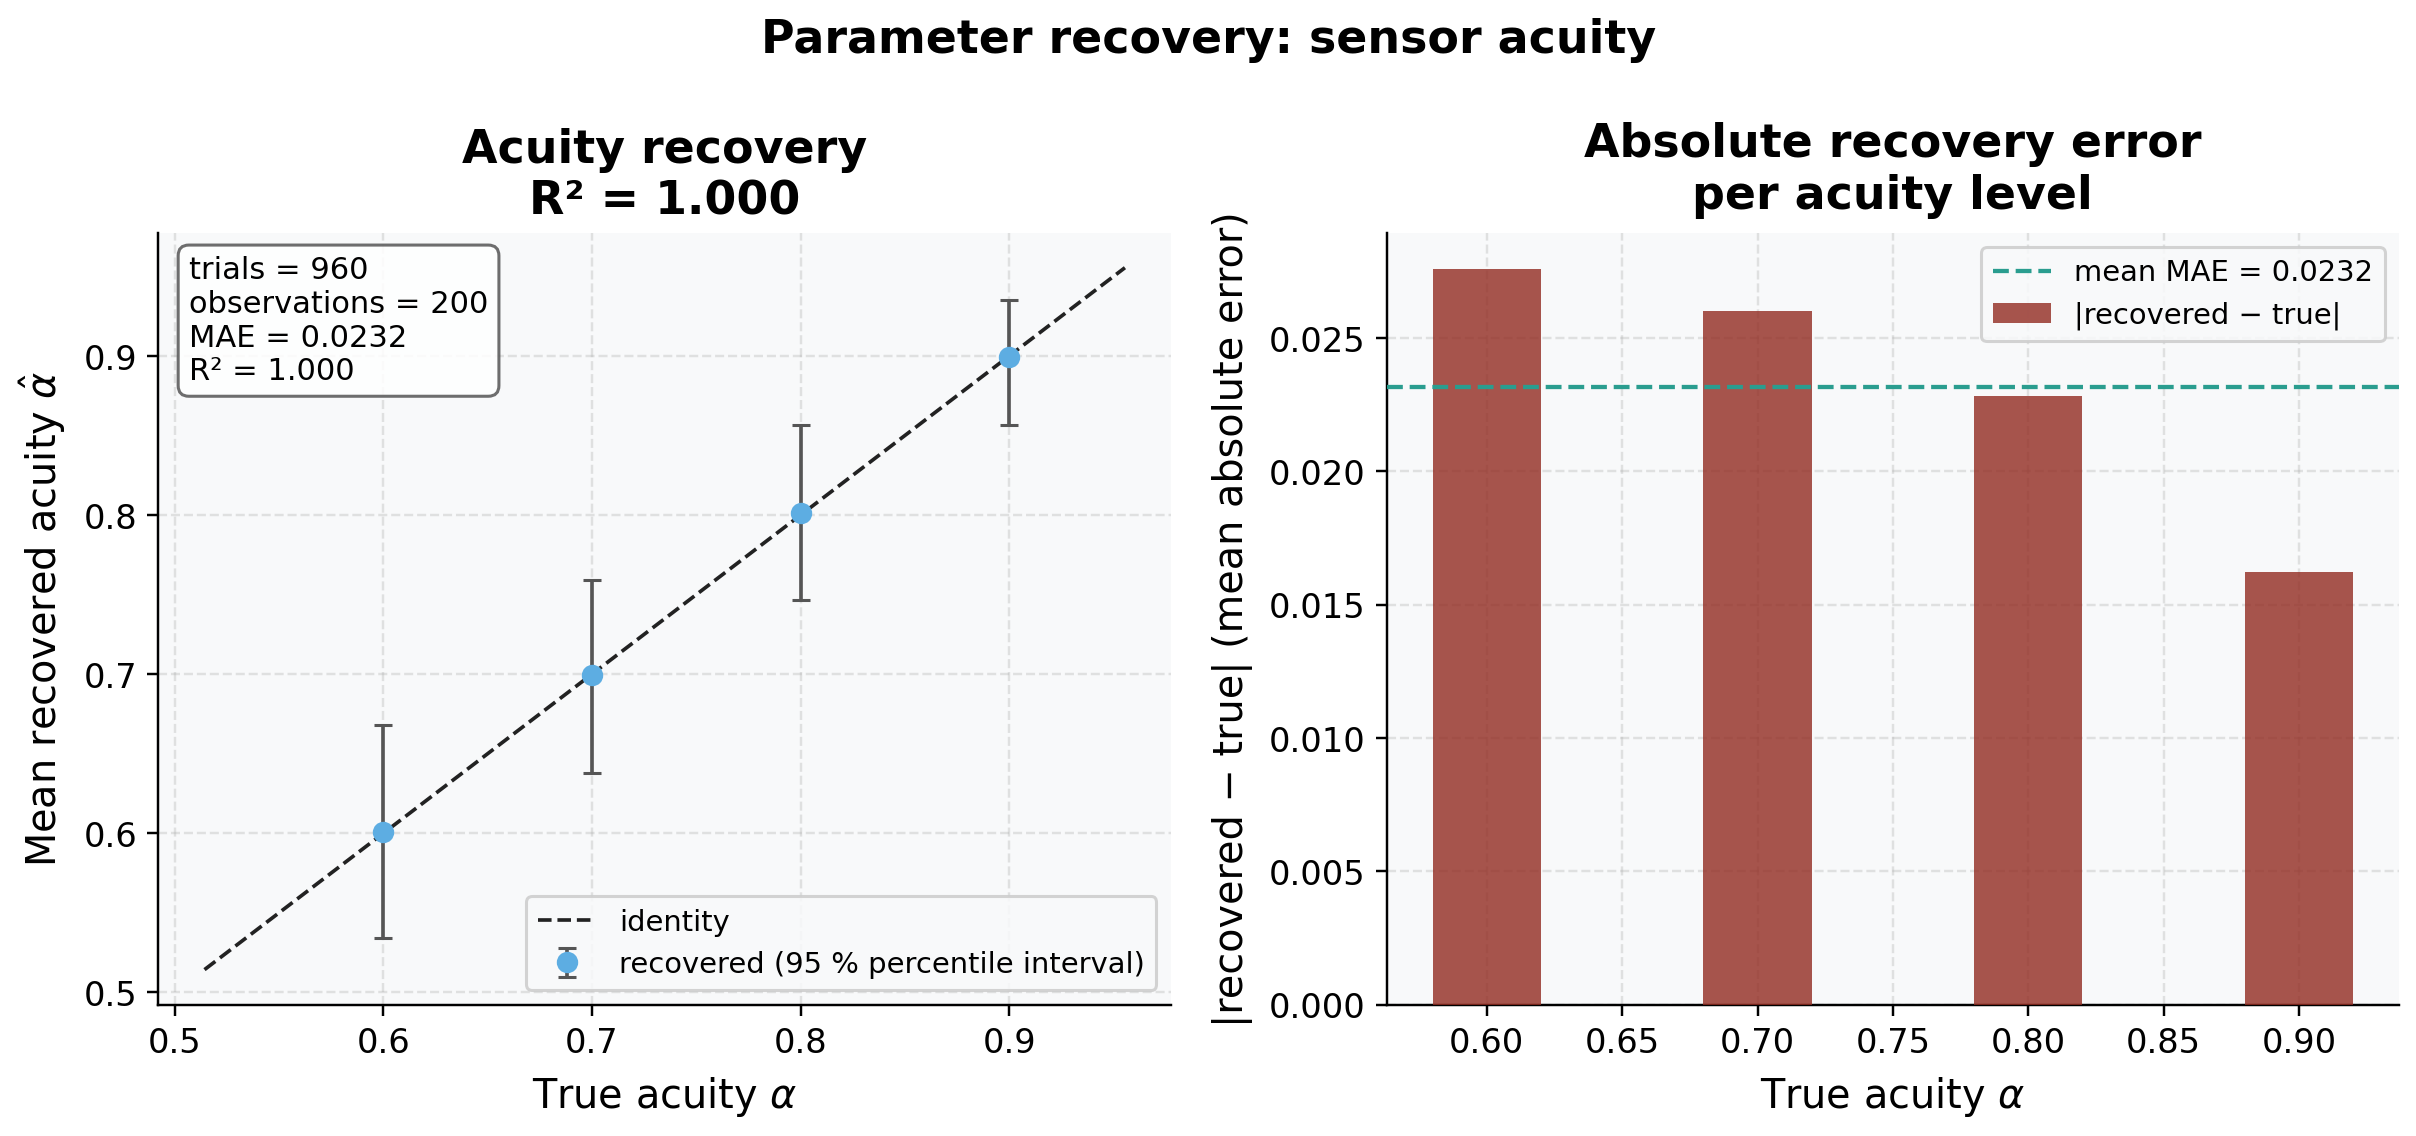
\includegraphics[width=0.9\linewidth,height=0.5\textheight,keepaspectratio,alt={Two-panel sensor-acuity recovery diagnostic. Open estimate markers with capped empirical intervals follow a dotted identity line; open dotted-hatch bars show absolute error at each tested acuity, with a labeled dotted rule for the global mean.}]{../figures/parameter_recovery.png}
\caption{Two-panel parameter-recovery diagnostic. Source relation:
original project parameter-recovery study; estimands: recovered acuity
and absolute error in probability units, plus the unitless coefficient
of determination \(R^2\) for mean recovered versus true acuity. In the
left panel, the x-axis is true acuity and the y-axis is mean recovered
acuity. Open estimate markers with capped error bars show the 95\%
empirical percentile interval across 960 independent synthetic trials
within each true-acuity grid point; the dark dotted diagonal is
identity, and the title reports \(R^2=0.9999\). This interval is a
descriptive quantile of independent-trial estimates, not a bootstrap
confidence interval or Bayesian credible interval. In the right panel,
the x-axis is tested true acuity and the y-axis is absolute acuity
error. Open dotted-hatch bars distinguish the errors without color, and
a labeled dark dotted rule marks global mean absolute error. Each trial
contains 200 nested observations. The configured seed initializes the
base RNG stream and is not the independent analysis unit. These
finite-grid estimates do not establish global structural identifiability
or recovery outside the tested observation
model.}\label{fig:parameter-recovery}
\end{figure}

\subsection{Hierarchical information-gating
diagnostic}\label{sec:results-hierarchical-bmr}

Study 7 shows that the 3-level agent runs and federates end to end. This
supplementary diagnostic asks a narrower question: under a configured
surprise threshold, does one leaf observation classify the top
meta-context as informative or non-gating? The output is a thresholded
information-gating diagnostic, not a Bayesian-model-evidence comparison
or a data-driven proof of the hierarchy's correct depth.

The implementation evaluates levels through
\breaktt{hierarchical\_reduce} in the \breaktt{bayesian\_model\_reduction}
module of \texttt{fedference}. For each non-leaf level we measure its
\textbf{Bayesian surprise} \(\mathrm{KL}(q_i \,\|\, \tilde p_i)\) ---
how far the leaf observation moves that level's belief \(q_i\) from its
top-down prior \(\tilde p_i\).

The routine labels a level below the configured threshold as prunable
and a level above it as kept. Because this is an inference-derived
divergence rather than a model re-fit, the labels are conditional on the
specified worlds, observation, and threshold.

The control is directional by construction. We build two 3-level worlds
that differ \emph{only} in the top level's conditioned priors: a
\textbf{degenerate} world whose meta-context is non-gating (both
meta-context states predict the same context distribution) and an
\textbf{informative} world whose meta-context sharply distinguishes the
two contexts.

In the degenerate world, the top level has Bayesian surprise 0.000 nats
and is flagged prunable (recovers the two-level structure: Yes). In the
informative world, it has 0.328 nats and is kept (Yes).

fig.~\ref{fig:hierarchical-bmr} shows both configured worlds side by
side. Their shared lower-level parameters isolate the top-level gating
contrast, but do not establish a generally correct depth-selection
procedure.

\begin{figure}
\centering
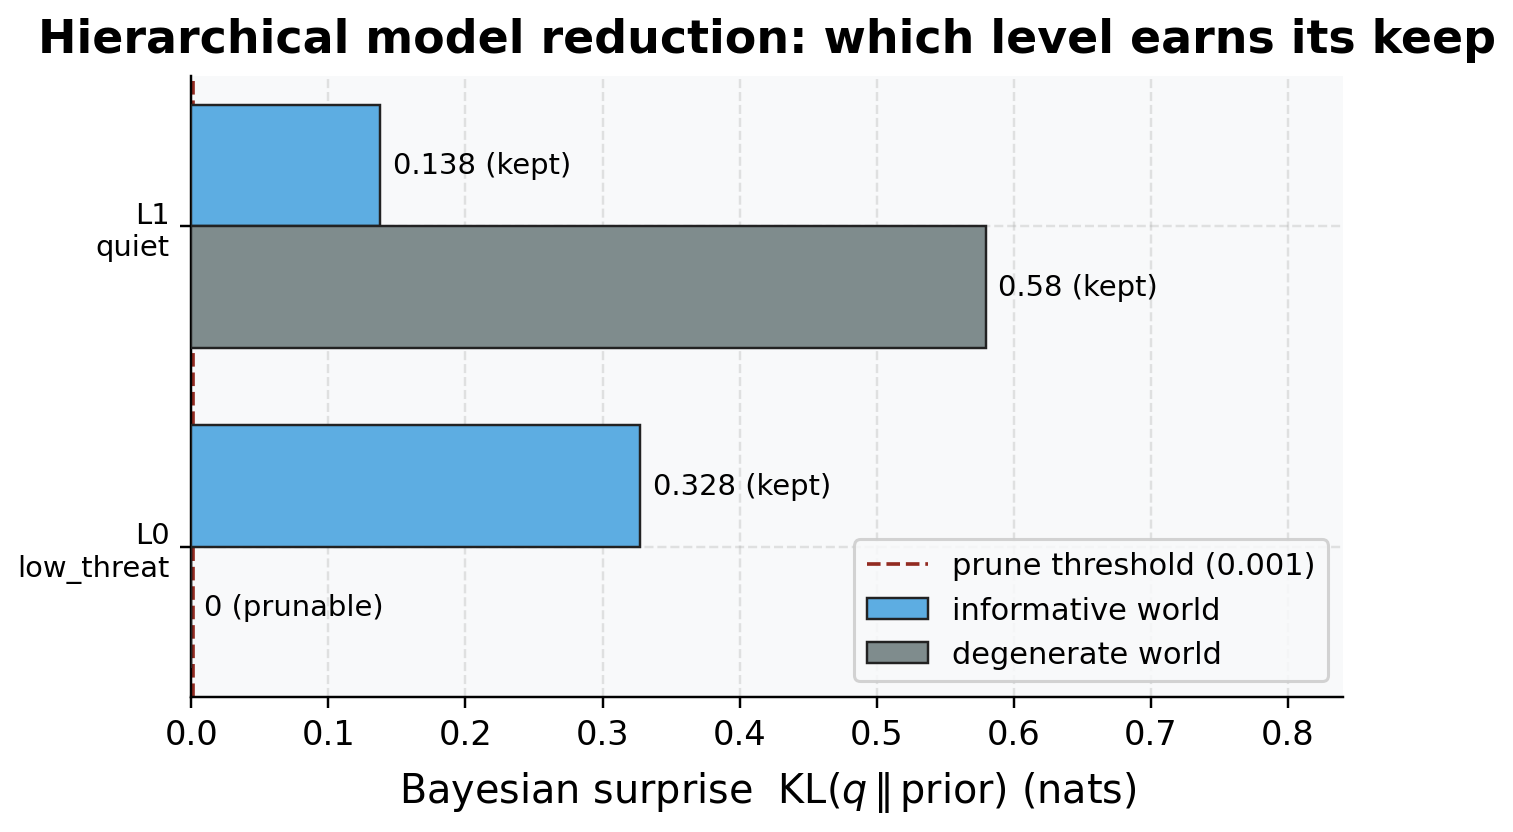
\includegraphics[width=0.8\linewidth,height=0.5\textheight,keepaspectratio,alt={Horizontal bars show Bayesian surprise at two non-leaf levels in informative and degenerate configured worlds. The threshold classifies whether the upper information channel is retained; this diagnostic is not a Bayesian-model-reduction emergence result.}]{../figures/hierarchical_bmr.png}
\caption{Per-level Bayesian surprise and configured threshold
classifications for two hierarchical worlds. Source relation: original
project information-gating diagnostic related to, but not an
implementation of, the BMR mechanism in Friston et al.~Fig. 9; estimand:
per-level Bayesian surprise in nats and its thresholded prune/keep
label; uncertainty: deterministic schematic worlds, so no resampling
interval applies. The x-axis is Bayesian surprise
\(\mathrm{KL}(q \,\|\, \text{prior})\) in nats, measuring information
added by the leaf observation. The y-axis lists the non-leaf reduction
targets top-down: level 0 is the meta-context (L3), level 1 is context
(L2), and leaf location L1 is not reduced. Hatches, keylines, direct
value-and-status labels, and vertical position distinguish the
informative and non-gating worlds without color; the dark dotted rule is
the declared classification threshold. The non-gating meta-context has
0.000 nats and is flagged prunable, leaving a two-level stack. The
informative meta-context has 0.328 nats and is kept; both worlds keep
context. The unit is nats for each configured world-level target, with
no independent replication unit, sample size, confidence interval, or
error band. Falling below the configured threshold is a sign-control
outcome, not proof of structural redundancy. The figure does not report
model evidence, posterior refitting, universal depth recovery, structure
emergence, or exact source-protocol
replication.}\label{fig:hierarchical-bmr}
\end{figure}

Unlike the Beta-function BMR sign control in
sec.~\ref{sec:results-emergence} and eq.~\ref{eq:bmr-deltaf}, this
routine thresholds per-level surprise. It therefore checks the intended
gating contrast in the declared worlds; it does not let the data
independently choose model depth.

\subsection{Sharp server heuristic: influence and finite-breakdown
characterization}\label{sec:results-heuristic-characterization}

The server-side \breaktt{robust\_aggregate} rule is the sharp heuristic
axis of the three-axes design (sec.~\ref{sec:robustness-axes-results}).
It has BH-rejected positive contrasts in the configured accuracy verdict
in sec.~\ref{sec:results-verdict} but has declared reversals elsewhere.

Unlike the objective-backed \breaktt{variational\_aggregate}, no
closed-form free-energy derivation has been established for it in this
repository. A separate scoped proposition in the aggregation-objective
supplement rules out the declared continuously differentiable, separable
forward-KL objective class for the implementation's raw log-pool block;
it does not rule out every broader coupled or fixed-point-only
construction.

The rule therefore remains a heuristic whose positive formal property is
bit-identical recovery of the log-linear pool at
\texttt{robustness\ =\ 0} (eq.~\ref{eq:robust-identity}). This section
does not promote the scoped negative result into an objective
certificate; it \emph{measures} the heuristic empirically, and the
measurement makes its honesty boundary concrete.

We measure two things (fig.~\ref{fig:heuristic-breakdown}). First, a
\textbf{numerical influence function}: we drag one agent's belief a
growing fraction toward a confident-wrong contamination point and read
its converged pooling weight. At \texttt{robustness\ =\ 0} the weight is
a flat \(1/n\) at every perturbation --- the naive pool never
down-weights anyone --- which anchors the instrument to the proven
recovery corner.

At positive robustness the dragged agent's influence falls (not strictly
monotonically --- a tiny drag can briefly \emph{raise} it before the
divergence penalty dominates, an honest non-monotonicity we report
rather than smooth away).

Second, and more consequentially, a \textbf{breakdown witness}. We add
colluding confident-wrong adversaries --- all broadcasting the same
false state --- to a fixed colony of 5 honest sentinels until each
aggregator's consensus argmax is \emph{captured} (flips to the
adversaries' target). The sharp heuristic is captured by 2 colluders;
the conservative objective-backed variational rule withstands more,
capitulating only at 4.

Both counts are \textbf{finite} (Yes): a colluding majority overwhelms
either rule. That finite breakdown point is the honest headline: neither
rule has an unconditional truth-recovery claim under coordinated
collusion. The absence of an objective theorem for
\breaktt{robust\_aggregate} is a separate derivational boundary.

The finite capture measurement neither establishes estimator-level
B-robustness nor refutes the variational rule's stated raw
effective-weight result.

The report also runs a declared diagnostic grid over state dimension,
honest-agent count, robustness, four simple attack mechanisms, and
balanced versus adversary-downweighted base weights. This is a coverage
instrument for finding counterexamples, not a random sample of worlds
and not a theorem search over all simplexes. A finite capture row is
evidence against a universal guarantee; an uncaptured row is only ``not
found within this search budget.''

\begin{figure}
\centering
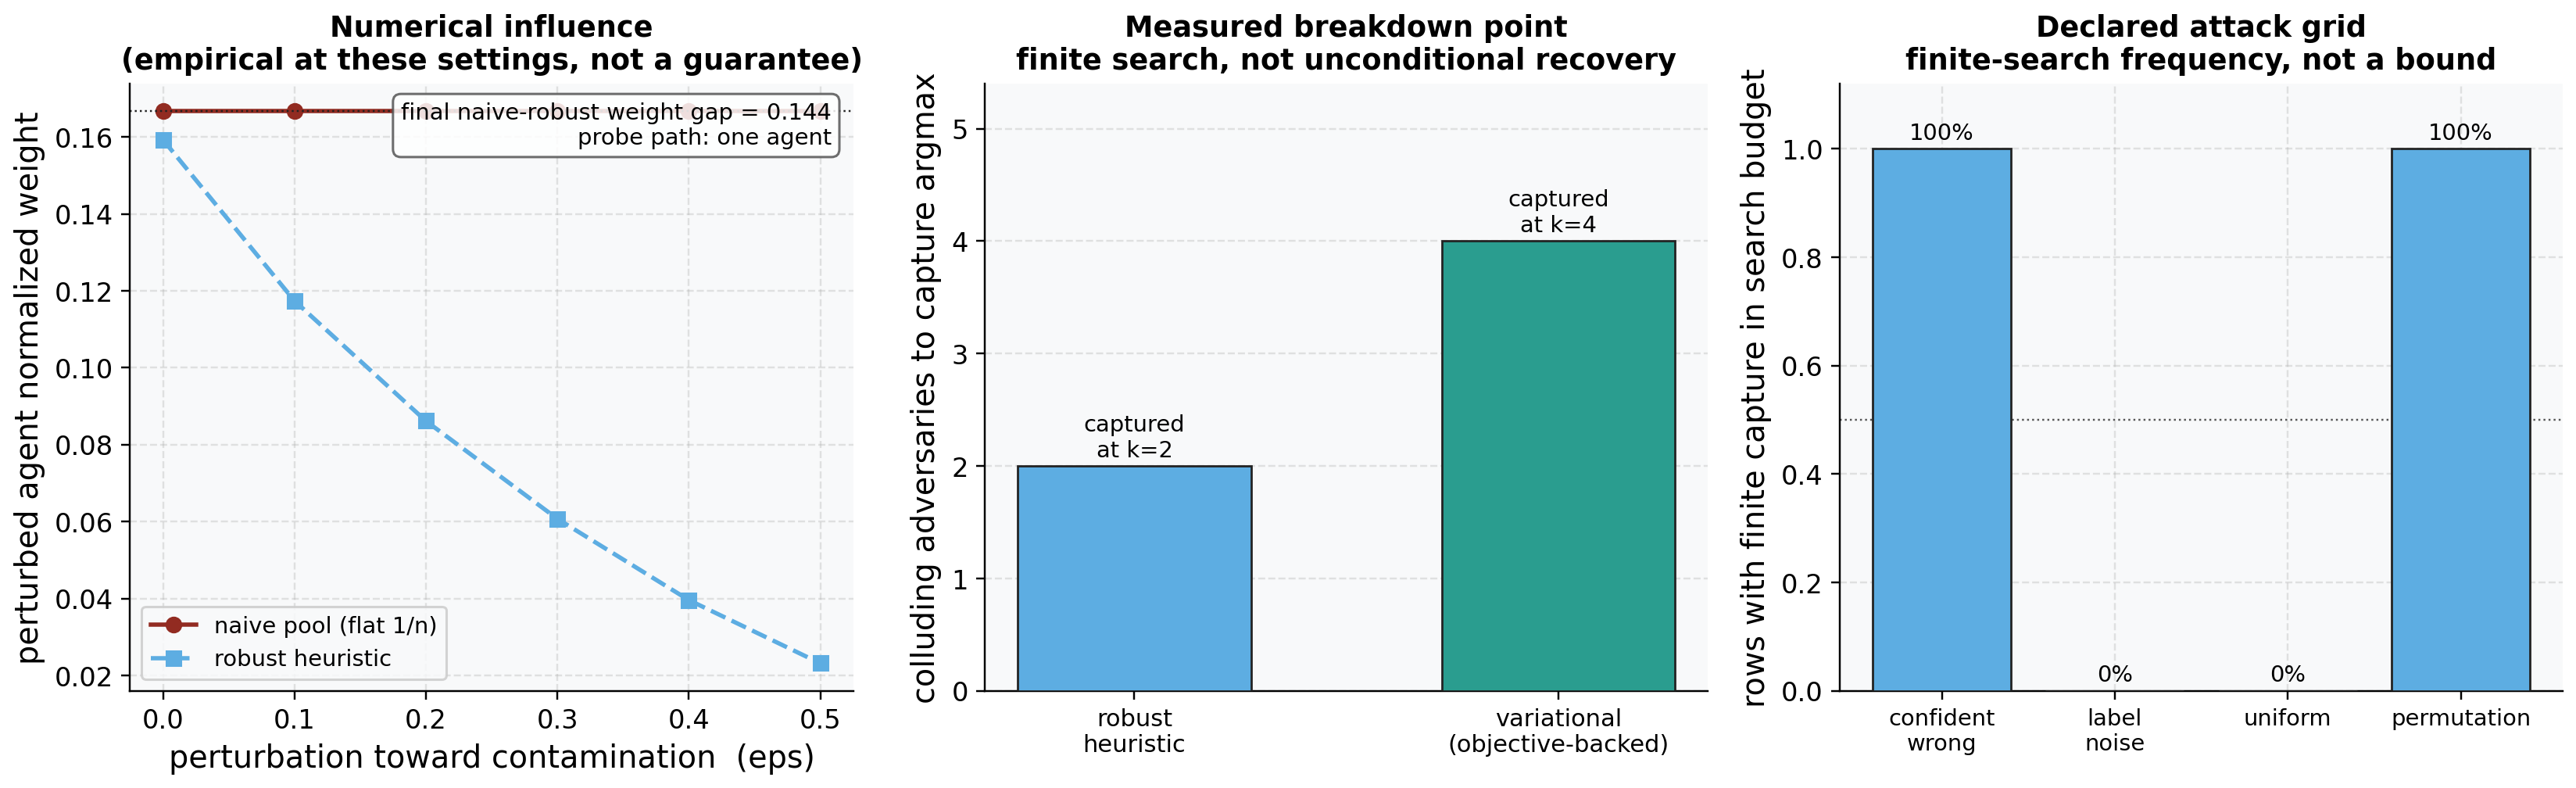
\includegraphics[width=0.95\linewidth,height=0.5\textheight,keepaspectratio,alt={Three-panel server-heuristic diagnostic: circle-solid versus square-dashed numerical influence, forward- versus dotted-hatch finite colluder counts for two aggregators, and directly labeled fractions of a declared attack grid with capture.}]{../figures/heuristic_breakdown.png}
\caption{Three-panel empirical characterization of the server-side
heuristic. Source relation: original project diagnostic of
\protect\breaktt{robust\_aggregate}; estimands: numerical influence,
finite-search capture count, and declared-grid capture fraction. In
Panel A, the x-axis is the perturbation fraction moving one agent toward
a confident-wrong belief and the y-axis is its converged normalized
pooling weight. Circle-solid and square-dashed paths distinguish the
naive pool and robust heuristic; a dark dotted rule marks \(1/n\), and a
direct arrow label gives the terminal gap. In Panel B, the x-axis is
aggregator and the y-axis is colluding-adversary count at
consensus-argmax capture: \(k=2\) for the heuristic and \(k=4\) for the
objective-backed variational rule. Forward and dotted hatches, dark
keylines, method names, and direct \protect\texttt{captured\ at\ k}
labels duplicate color. Panel C's x-axis is declared attack mechanism
and its y-axis is the fraction of searched rows with finite capture
inside the configured budget; direct percentages identify each bar.
Units are normalized weight, adversary count, and finite-grid fraction.
This is a deterministic finite grid with no population resampling; each
declared seeded scenario row is a computational unit, not an
exchangeable population replicate, so no confidence interval is shown.
The grid fraction is neither a probability nor a global breakdown bound,
and these settings do not establish bounded influence, Byzantine
tolerance, or universal robustness.}\label{fig:heuristic-breakdown}
\end{figure}

\section{References}\label{sec:references}

The bibliography lives in
\href{https://github.com/ActiveInferenceInstitute/Active_Fedference/blob/main/manuscript/references.bib}{project
bibliography source} and is read by Pandoc during rendering. The
combined PDF path invokes \texttt{-\/-natbib}, so citation markers
become LaTeX citation commands resolved against the bib file. HTML,
reveal.js, and other non-LaTeX reader surfaces use \texttt{-\/-citeproc}
against that same file. This is one bibliography with format-specific
consumers, not two metadata sources. Titles retain the source's original
spelling.

The standalone checkout provides a local cross-reference gate for
citation labels and all manuscript references:

\begin{Shaded}
\begin{Highlighting}[]
\ExtensionTok{uv}\NormalTok{ run }\AttributeTok{{-}{-}locked}\NormalTok{ pytest tests/test\_xref\_integrity.py }\AttributeTok{{-}q}
\end{Highlighting}
\end{Shaded}

To validate that \texttt{references.bib} is syntactically clean and
contains the required fields per entry type, the stricter citation
validator is available when the project is checked out under the
template monorepo's \breaktt{projects/working/} (it is not on the
standalone repo's own dependency graph), invoked from the monorepo root
with a monorepo-relative path:

\begin{Shaded}
\begin{Highlighting}[]
\VariableTok{p}\OperatorTok{=}\NormalTok{projects/working/}\DataTypeTok{\textbackslash{}}
\NormalTok{active\_fedference}
\VariableTok{b}\OperatorTok{=}\VariableTok{$p}\NormalTok{/manuscript/references.bib}
\ExtensionTok{uv}\NormalTok{ run python }\AttributeTok{{-}m} \DataTypeTok{\textbackslash{}}
\NormalTok{  infrastructure.reference.}\DataTypeTok{\textbackslash{}}
\NormalTok{citation.cli validate }\StringTok{"}\VariableTok{$b}\StringTok{"} \AttributeTok{{-}{-}strict}
\end{Highlighting}
\end{Shaded}




\providecommand{\bibsection}{}
\renewcommand{\bibsection}{}

\bibliography{references}
\end{document}
